
\documentclass[a4paper,12pt,twoside]{report}
%\documentclass[a4paper,11pt,twoside]{memoir}


%cite package
%\usepackage{cite}

\usepackage{tikz}
\usepackage{amsmath}
\usepackage{multicol}
\usepackage{multirow}
\usepackage{textgreek}
\usepackage{float}
\usepackage{graphicx}


%\usepackage[square,numbers]{natbib}
%\usepackage[backend=biber]{biblatex}

\usepackage[dashed=false,
backend=biber,
style=ieee,
bibencoding=ascii,
sortcites=true,
citestyle=numeric-comp
%style=alphabetic
%style=reading
]{biblatex}

%BIBTEX URL BREAK
\setcounter{biburllcpenalty}{7000}
\setcounter{biburlucpenalty}{7000}
\setcounter{biburlnumpenalty}{7000}

%Appendix package
\usepackage[title]{appendix}
%Sideways table package
\usepackage{rotating}

%\usepackage[backend=biber,style=ieee,natbib=true]{biblatex} 

\addbibresource{bibliography/bibliography.bib}

%%%%CMS AN subfigures%%%%%%%%%
\usepackage{fancyhdr}%        modern version of fancyheadings
\usepackage{subfig}%
\let\subfigure\subfloat% compatibility between subfigure and subfig packages

%\usepackage[left=2cm,right=2cm,top=2cm,bottom=3cm]{geometry}
\usepackage[a4paper, width=150mm, top=25mm, bottom=25mm]{geometry} % -- use for printing
%\usepackage[top=2.5cm, bottom=1.8cm,left=4.0cm,right=1.5cm]{geometry} % --- Dwayne's



\usepackage{graphicx}
\usepackage{verbatim}
\usepackage{latexsym}
\usepackage{mathchars}
\usepackage{setspace}

\setlength{\parskip}{\medskipamount}  % a little space before a \par
\setlength{\parindent}{0pt}	      % don't indent first lines of paragraphs

%UHEAD.STY  If this is included after \documentstyle{report}, it adds
% an underlined heading style to the LaTeX report style.
% \pagestyle{uheadings} will put underlined headings at the top
% of each page. The right page headings are the Chapter titles and
% the left page titles are supplied by \def\lefthead{text}.

% Ted Shapin, Dec. 17, 1986

\makeatletter
\def\chapapp2{Chapter}

\def\appendix{\par
 \setcounter{chapter}{0}
 \setcounter{section}{0}
 \def\chapapp2{Appendix}
 \def\@chapapp{Appendix}
 \def\thechapter{\Alph{chapter}}}

\def\ps@uheadings{\let\@mkboth\markboth
% modifications
\def\@oddhead{\protect\underline{\protect\makebox[\textwidth][l]
		{\sl\rightmark\hfill\rm\thepage}}}
\def\@oddfoot{}
\def\@evenfoot{}
\def\@evenhead{\protect\underline{\protect\makebox[\textwidth][l]
		{\rm\thepage\hfill\sl\leftmark}}}
% end of modifications
\def\chaptermark##1{\markboth {\ifnum \c@secnumdepth >\m@ne
 \chapapp2\ \thechapter. \ \fi ##1}{}}%
\def\sectionmark##1{\markright {\ifnum \c@secnumdepth >\z@
   \thesection. \ \fi ##1}}}
\makeatother



%%From: marcel@cs.caltech.edu (Marcel van der Goot)
%%Newsgroups: comp.text.tex
%%Subject: illegal modification of boxit.sty
%%Date: 28 Feb 92 01:10:02 GMT
%%Organization: California Institute of Technology (CS dept)
%%Nntp-Posting-Host: andromeda.cs.caltech.edu
%%
%%
%%Quite some time ago I posted a file boxit.sty; maybe it made it
%%to some archives, although I don't recall submitting it. It defines
%%	\begin{boxit}
%%	...
%%	\end{boxit}
%%to draw a box around `...', where the `...' can contain other
%%environments (e.g., a verbatim environment). Unfortunately, it had
%%a problem: it did not work if you used it in paragraph mode, i.e., it
%%only worked if there was an empty line in front of \begin{boxit}.
%%Luckily, that is easily corrected.
%%
%%HOWEVER, apparently someone noticed the problem, tried to correct it,
%%and then distributed this modified version. That would be fine with me,
%%except that:
%%1. There was no note in the file about this modification, it only has my
%%   name in it.
%%2. The modification is wrong: now it only works if there is *no* empty
%%   line in front of \begin{boxit}. In my opinion this bug is worse than
%%   the original one.
%%
%%In particular, the author of this modification tried to force an empty
%%line by inserting a `\\' in the definition of \Beginboxit. If you have
%%a version of boxit.sty with a `\\', please delete it. If you have my
%%old version of boxit.sty, please also delete it. Below is an improved
%%version.
%%
%%Thanks to Joe Armstrong for drawing my attention to the bug and to the
%%illegal version.
%%
%%                                          Marcel van der Goot
%% .---------------------------------------------------------------
%% | Blauw de viooltjes,                    marcel@cs.caltech.edu
%% |    Rood zijn de rozen;
%% | Een rijm kan gezet
%% |    Met plaksel en dozen.
%% |


% boxit.sty
% version: 27 Feb 1992
%
% Defines a boxit environment, which draws lines around its contents.
% Usage:
%   \begin{boxit}
%	... (text you want to be boxed, can contain other environments)
%   \end{boxit}
%
% The width of the box is the width of the contents.
% The boxit* environment behaves the same, except that the box will be
% at least as wide as a normal paragraph.
%
% The reason for writing it this way (rather than with the \boxit#1 macro
% from the TeXbook), is that now you can box verbatim text, as in
%   \begin{boxit}
%   \begin{verbatim}
%   this better come out in boxed verbatim mode ...
%   \end{verbatim}
%   \end{boxit}
%
%						Marcel van der Goot
%						marcel@cs.caltech.edu
%

\def\Beginboxit
   {\par
    \vbox\bgroup
	   \hrule
	   \hbox\bgroup
		  \vrule \kern1.2pt %
		  \vbox\bgroup\kern1.2pt
   }

\def\Endboxit{%
			      \kern1.2pt
		       \egroup
		  \kern1.2pt\vrule
		\egroup
	   \hrule
	 \egroup
   }	

\newenvironment{boxit}{\Beginboxit}{\Endboxit}
\newenvironment{boxit*}{\Beginboxit\hbox to\hsize{}}{\Endboxit}

\pagestyle{empty}

\setlength{\parskip}{2ex plus 0.5ex minus 0.2ex}
\setlength{\parindent}{0pt}

\makeatletter  %to avoid error messages generated by "\@". Makes Latex treat "@" like a letter

\linespread{1.5}
\def\submitdate#1{\gdef\@submitdate{#1}}

\def\maketitle{
  \begin{titlepage}{
    %\linespread{1.5}
    \Large University of London \\
    %\linebreak
    Imperial College of Science, Technology and Medicine \\
    %\linebreak
    Department of Physics
    \rm
    \vskip 3in
    \Large \bf \@title \par
  }
  \vskip 0.3in
  \par
  {\Large \@author}
  \vskip 4in
  \par
  Submitted in part fulfilment of the requirements for the degree of 
  \linebreak
  Doctor of Philosophy in Physics of the University of London and 
  \linebreak
  the Diploma of Imperial College, \@submitdate
  \vfil
  \end{titlepage}
}

\def\titlepage{
  \newpage
  \centering
  \linespread{1}
  \normalsize
  \vbox to \vsize\bgroup\vbox to 9in\bgroup
}
\def\endtitlepage{
  \par
  \kern 0pt
  \egroup
  \vss
  \egroup
  \cleardoublepage
}

\def\abstract{
  \begin{center}{
    \large\bf Abstract}
  \end{center}
  \small
  %\def\baselinestretch{1.5}
  \linespread{1.5}
  \normalsize
}
\def\endabstract{
  \par
}

\newenvironment{acknowledgements}{
  \cleardoublepage
  \begin{center}{
    \large \bf Acknowledgements}
  \end{center}
  \small
  \linespread{1.5}
  \normalsize
}{\cleardoublepage}
\def\endacknowledgements{
  \par
}

\newenvironment{dedication}{
  \cleardoublepage
  \begin{center}{
    \large \bf Dedication}
  \end{center}
  \small
  \linespread{1.5}
  \normalsize
}{\cleardoublepage}
\def\enddedication{
  \par
}

\def\preface{
    \pagenumbering{roman}
    \pagestyle{plain}
    \doublespacing
}

\def\body{
    \cleardoublepage    
    \pagestyle{uheadings}
    \tableofcontents
    \pagestyle{plain}
    \cleardoublepage
    \pagestyle{uheadings}
    \listoftables
    \pagestyle{plain}
    \cleardoublepage
    \pagestyle{uheadings}
    \listoffigures
    \pagestyle{plain}
    \cleardoublepage
    \pagestyle{uheadings}
    \pagenumbering{arabic}
    \doublespacing
}

\makeatother  %to avoid error messages generated by "\@". Makes Latex treat "@" like a letter


\newcommand{\ipc}{{\sf ipc}}

\newcommand{\Prob}{\bbbp}
\newcommand{\Real}{\bbbr}
\newcommand{\real}{\Real}
\newcommand{\Int}{\bbbz}
\newcommand{\Nat}{\bbbn}

\newcommand{\NN}{{\sf I\kern-0.14emN}}   % Natural numbers
\newcommand{\ZZ}{{\sf Z\kern-0.45emZ}}   % Integers
\newcommand{\QQQ}{{\sf C\kern-0.48emQ}}   % Rational numbers
\newcommand{\RR}{{\sf I\kern-0.14emR}}   % Real numbers
\newcommand{\KK}{{\cal K}}
\newcommand{\OO}{{\cal O}}
\newcommand{\AAA}{{\bf A}}
\newcommand{\HH}{{\bf H}}
\newcommand{\II}{{\bf I}}
\newcommand{\LL}{{\bf L}}
\newcommand{\PP}{{\bf P}}
\newcommand{\PPprime}{{\bf P'}}
\newcommand{\QQ}{{\bf Q}}
\newcommand{\UU}{{\bf U}}
\newcommand{\UUprime}{{\bf U'}}
\newcommand{\zzero}{{\bf 0}}
\newcommand{\ppi}{\mbox{\boldmath $\pi$}}
\newcommand{\aalph}{\mbox{\boldmath $\alpha$}}
\newcommand{\bb}{{\bf b}}
\newcommand{\ee}{{\bf e}}
\newcommand{\mmu}{\mbox{\boldmath $\mu$}}
\newcommand{\vv}{{\bf v}}
\newcommand{\xx}{{\bf x}}
\newcommand{\yy}{{\bf y}}
\newcommand{\zz}{{\bf z}}
\newcommand{\oomeg}{\mbox{\boldmath $\omega$}}
\newcommand{\res}{{\bf res}}
\newcommand{\cchi}{{\mbox{\raisebox{.4ex}{$\chi$}}}}
%\newcommand{\cchi}{{\cal X}}
%\newcommand{\cchi}{\mbox{\Large $\chi$}}

% Logical operators and symbols
\newcommand{\imply}{\Rightarrow}
\newcommand{\bimply}{\Leftrightarrow}
\newcommand{\union}{\cup}
\newcommand{\intersect}{\cap}
\newcommand{\boolor}{\vee}
\newcommand{\booland}{\wedge}
\newcommand{\boolimply}{\imply}
\newcommand{\boolbimply}{\bimply}
\newcommand{\boolnot}{\neg}
\newcommand{\boolsat}{\!\models}
\newcommand{\boolnsat}{\!\not\models}


\newcommand{\op}[1]{\mathrm{#1}}
\newcommand{\s}[1]{\ensuremath{\mathcal #1}}

% Properly styled differentiation and integration operators
\newcommand{\diff}[1]{\mathrm{\frac{d}{d\mathit{#1}}}}
\newcommand{\diffII}[1]{\mathrm{\frac{d^2}{d\mathit{#1}^2}}}
\newcommand{\intg}[4]{\int_{#3}^{#4} #1 \, \mathrm{d}#2}
\newcommand{\intgd}[4]{\int\!\!\!\!\int_{#4} #1 \, \mathrm{d}#2 \, \mathrm{d}#3}

% Large () brackets on different lines of an eqnarray environment
\newcommand{\Leftbrace}[1]{\left(\raisebox{0mm}[#1][#1]{}\right.}
\newcommand{\Rightbrace}[1]{\left.\raisebox{0mm}[#1][#1]{}\right)}

% Funky symobols for footnotes
\newcommand{\symbolfootnote}{\renewcommand{\thefootnote}{\fnsymbol{footnote}}}
% now add \symbolfootnote to the beginning of the document...
\newcommand{\doubleinespacing}{\renewcommand{\baselinestretch}{2.0} \normalsize}
\newcommand{\normallinespacing}{\renewcommand{\baselinestretch}{1.5} \normalsize}
\newcommand{\mediumlinespacing}{\renewcommand{\baselinestretch}{1.2} \normalsize}
\newcommand{\narrowlinespacing}{\renewcommand{\baselinestretch}{1.0} \normalsize}
\newcommand{\bump}{\noalign{\vspace*{\doublerulesep}}}
\newcommand{\cell}{\multicolumn{1}{}{}}
\newcommand{\spann}{\mbox{span}}
\newcommand{\diagg}{\mbox{diag}}
\newcommand{\modd}{\mbox{mod}}
\newcommand{\minn}{\mbox{min}}
\newcommand{\andd}{\mbox{and}}
\newcommand{\forr}{\mbox{for}}
\newcommand{\EE}{\mbox{E}}

\newcommand{\deff}{\stackrel{\mathrm{def}}{=}}
\newcommand{\syncc}{~\stackrel{\textstyle \rhd\kern-0.57em\lhd}{\scriptstyle L}~}

\def\coop{\mbox{\large $\rhd\!\!\!\lhd$}}
\newcommand{\sync}[1]{\raisebox{-1.0ex}{$\;\stackrel{\coop}{\scriptscriptstyle
#1}\,$}}

\newtheorem{definition}{Definition}[chapter]
\newtheorem{theorem}{Theorem}[chapter]

\newcommand{\Figref}[1]{Figure~\ref{#1}}
\newcommand{\fig}[3]{
 \begin{figure}[!ht]
 \begin{center}
 \scalebox{#3}{\includegraphics{figs/#1.ps}}
 \vspace{-0.1in}
 \caption[ ]{\label{#1} #2}
 \end{center}
 \end{figure}
}

\newcommand{\figtwo}[8]{
 \begin{figure}
 \parbox[b]{#4 \textwidth}{
 \begin{center}
 \scalebox{#3}{\includegraphics{figs/#1.ps}}
 \vspace{-0.1in}
 \caption{\label{#1}#2}
 \end{center}
 }
 \hfill
 \parbox[b]{#8 \textwidth}{
 \begin{center}
 \scalebox{#7}{\includegraphics{figs/#5.ps}}
 \vspace{-0.1in}
 \caption{\label{#5}#6}
 \end{center}
 }
 \end{figure}
}


\usepackage{color}   %May be necessary if you want to color links
\usepackage{hyperref}
\hypersetup{
    colorlinks=false, %set true if you want colored links
    linktoc=all,     %set to all if you want both sections and subsections linked
    linkcolor=blue,  %choose some color if you want links to stand out
}

% Removes two space start of a new sentence
%\frenchspacing
% Returns to one
%chapter ornaments test
\usepackage{xcolor}
\usepackage{titlesec}
\usepackage{lmodern}
\usepackage{tikz}
\usepackage{pgfornament}
\usetikzlibrary{calc}
\usepackage{setspace}
%\usepackage{ebgaramond}

%%%%%%%%%%%%%%%%LINE NUMBERING%%%%%%%%%%%%%%%%%%
\usepackage{lineno}
%\linenumbers

 %%%%%%%%%%%%%%%%%%%%%%%%%%%%%%%%%%%
%%%%%%%%%%%%%%%%%%%%%%%%%%%CMS AN FONT%%%%%%%%%%%%%%%%
%\usepackage{palatino}
%%%%%%%%%%%%%%%%%%%%%%%%%%%CMS AN FONT%%%%%%%%%%%%%%%%






%Styling test
\usepackage{fancyhdr}
\usepackage{lettrine}
\input Acorn.fd
\newcommand*\initfamily{\usefont{U}{Acorn}{xl}{n}}
%Test end

%Quotes
\usepackage{epigraph}
%\epigraphfontsize{\small\itshape}
\setlength\epigraphwidth{8cm}
%\setlength\epigraphwidth{.8\textwidth}
\setlength\epigraphrule{0pt}

%\normallinespacing
\mediumlinespacing
%\doubleinespacing

%CHAPTER STYLE




%old working setup
%\bibliography{bibliography/bibliography}

%DEFINE COMMANDS - MATH

\newcommand{\MET}{$E_{T,miss}$}
\newcommand{\METnolep}{$E_{T,miss}^{no, l}$}
\newcommand{\METnomu}{$E_{T,miss}^{no, \mu}$}
\newcommand{\METnoe}{$E_{T,miss}^{no, e}$}
\newcommand{\mindphi}{$min\Delta\phi(j,E_{T,miss})$}
\newcommand{\mindphinolep}{$min\Delta\phi(j,E_{T,miss}^{no, l})$}
\newcommand{\mindphinomu}{$min\Delta\phi(j,E_{T,miss}^{no, \mu})$}
\newcommand{\mindphinoe}{$min\Delta\phi(j,E_{T,miss}^{no, e})$}

%Define checkmark
\def\checkmark{\tikz\fill[scale=0.4](0,.35) -- (.25,0) -- (1,.7) -- (.25,.15) -- cycle;} 


\begin{document}


\title{\Large {\bf Search for invisible decays of the Higgs boson at $\sqrt{s}$ = 13~TeV}\\
 \vspace*{6mm}
}

\author{\large Vuka\v sin Milo\v sevi\' c}
\submitdate{August 2020}



\maketitle
\preface


\addcontentsline{toc}{chapter}{Abstract}

\begin{abstract}
\mediumlinespacing
A search for invisibly decaying Higgs bosons using proton proton collision data collected by the CMS experiment at $\sqrt{s}=$~13~TeV is presented. For the first time, this search is performed using the full Run-2 dataset, corresponding to an integrated luminosity of 137.2~fb$^{-1}$. 

\hspace{10pt} In 2017 and 2018, to supplement the traditional trigger strategy based on the presence of missing transverse energy, a new dedicated trigger based on the Vector Boson Fusion jet topology was introduced. Its motivation, implementation and subsequent usage is described in detail in this thesis. Its addition further enhanced the sensitivity to the Vector Boson Fusion production mechanism by allowing for a new analysis category focused around previously inaccessible event.

\hspace{10pt} A combination with the study focusing on the 2016 data is performed. No deviations from the Standard Model have been observed and the final result is reported in the form of a 95~\% Confidence Level upper limit on the Br(H$\rightarrow$inv). The overall result from the full Run-2 phase of operation is presented to be Br(H$\rightarrow$inv)~$<$~XX (XX) observed (expected). When interpreted in terms of Dark Matter searches, this result provides a leading upper limit result for sub $m_H/2$ Dark Matter candidates. Lastly, a study of projected sensitivity of this study for the conditions provided by the future upgrades of the CMS experiment is also presented.The projected limit for the total integrated luminosity of 3000 $fb^{-1}$ is placed at from the perspective of the CMS experiment at Br(H$\rightarrow$inv)~$<$~4.5 \%, while a combined result from the ATLAS and CMS experiments is expected to be Br(H$\rightarrow$inv)~$<$~2.5 \%.

\end{abstract}

\cleardoublepage
\begin{copyright}
\mediumlinespacing
The copyright of this thesis rests with the author and is made available under a Creative Commons Attribution Non-Commercial No Derivatives licence. Researchers are free to copy, distribute or transmit the thesis on the condition that they attribute it, that they do not use it for commercial purposes and that they do not alter, transform or build upon it. For any reuse or redistribution, researchers must make clear to others the licence terms of this work.
\end{copyright}

\cleardoublepage

\addcontentsline{toc}{chapter}{Acknowledgements}

\begin{acknowledgements}

I would like to express (whatever feelings I have) to:

\begin{itemize}
 \item My supervisor
 \vspace*{3mm}
 \item My second supervisor
 \vspace*{3mm}
 \item Other researchers
 \vspace*{3mm}
 \item My family and friends
\end{itemize}

\end{acknowledgements}


\cleardoublepage

\begin{dedication}
  Dedication here.
\end{dedication}


\clearpage

\narrowlinespacing

\vspace*{4mm}
``I do not fear invisible worlds."\\
%`Quote text here.'\\
%\\
\emph{Ivo Andri\' c}

%\epigraph{\itshape``I do not fear invisible worlds."}{--- \textup{Ivo Andri\' c}}

\normallinespacing


\body


%\part[The Idea]{The Idea \\
%%                  \begin{center}
 %                    \begin{minipage}[l]{11cm}
 %%                     \textnormal{\normalsize **Proba kako izgleda**}
  %                   \end{minipage}
  %                    \end{center}}
                 
%\part[The Idea]{ \begin{center}
%                   \begin{minipage}{1.0\textwidth}
%                     \begin{tikzpicture}[remember picture, overlay]
%%                        \node[inner sep=6pt] (chapter) at (current page.center){\Huge The Experiment};
 %                       \node[inner sep=12pt, below of=chapter, text width=10cm, align=center, outer sep=12pt] (title1) {\textnormal{\large \textit{``Bez alata nema zanata."}}};
%                        \node[inner sep=12pt, below of=title1, text width=10cm, align=center, outer sep=6pt] (title) {\textnormal{\large-- \textup{Srpska narodna izreka} --}};
%                     \node[anchor=north] at (title.south){\pgfornament[width=5cm]{87}};
%                     \node[anchor=south] at (chapter.north){\pgfornament[width=3.5cm,symmetry=h]{81}};
%                     \end{tikzpicture} 
%                   \end{minipage}
%                 \end{center}
%                 }                  
                  
                  
%\setcounter{chapter}{-1}
\chapter*{Overview and declaration}
\mediumlinespacing

\hspace{10pt}\lettrine[lines=2]{\initfamily{T}}{he following document} serves as the summary of my work during the past four years. All other statements and results are appropriately referenced. Based on the conventional thesis structure, Chapter~\ref{ch:theory} presents a description of the main pieces forming the most complete particle physics theory, the Standard Model. This is  followed by a description of the idea for connecting the invisible final state of the Higgs Boson with the prospects for Dark Matter searches, formulated into Chapter~\ref{ch:Higgs_LHC_DM}. The two aforementioned chapters form Part I of this thesis, and serve as a theoretical/motivation basis, explained in my own words, allowing the reader to have a brief theory overview before moving forward with the details of the experimental approach. 

\hspace{10pt} Part II of this thesis serves as an introduction to the world of collider physics with the emphasis on the structure of the CMS experiment (Chapter~\ref{ch:cms_experiment}) as well as a description of its data acquisition system (Chapter~\ref{ch:daq}). Chapter 4 contains an overview of the Data Quality Monitoring system for the Level-1 trigger within the CMS experiment with an example being given in the form the Level-1 Trigger Calorimeter Layer 2. This section includes my work during the 2017-2018 period of data taking, when I was in charge of developing and maintaining that system. Chapter~\ref{ch:daq} also contains a detailed description of the implementation of High Level Trigger paths designed specifically for the purposes of the main study covered by this thesis. This part serves as a summary of my work on this topic, as I was responsible for the design, development, implementation and testing of those paths.

\hspace{10pt} Part III presents the main results given in this thesis, the search for invisible decays of the Higgs boson at $\sqrt{s}=$~13~TeV. The focus of this thesis is the scenario in which the Higgs Boson is produced through the process of Vector Boson Fusion. Chapter~\ref{ch:objects} serves as an overview of algorithms deployed for the purpose of particle reconstruction followed with a discussion of respective object corrections (some of which were developed for this study specifically by the Imperial College analysis team). Chapters~\ref{ch:an_strategy} and~\ref{ch:control_regions} introduce the main strategy behind this study. Having been its lead analyser (and publication contact), these chapters showcase my work, performed as a member of the Imperial College analysis team. The overview of the treatment of uncertainties and the signal extraction strategy begins the discussion presented in Chapter~\ref{ch:fit}, which culminates with a summary of final results that came out of this search. This summary focuses on the benefits gained through the use of the full dataset collected by the CMS detector during the 2017-2018 period and a novel approach to the analysis strategy with the usage of new triggers. Combination with the previously published results based on the data collected during 2016 is also presented yielding a preliminary legacy result for this study.

\hspace{10pt} Lastly, Chapter~\ref{ch:conclusion} serves as a conclusion of the journey summarised in this thesis. It is used to present final statements on the main analysis presented in previous chapters as well as to indicate what the future may hold. The prospects for the near future include the strategy for the combination of different searches for the invisible final state of the Higgs boson, where the previously described results focusing on the Vector Boson Fusion production mode are going to be combined with results from studies targeting other hadronic production modes. This section will summarise my work as a member of a UK wide collaboration of analysis teams forming the "Combined Higgs to Invisible Project" (CHIP) working group. Before concluding, a simulation study of future prospects for these analyses is presented, covering part of my work done in order to test the sensitivity of these processes and the behaviour of the upgraded CMS detector under expected future operation conditions of the Large Hadron Collider.

 \tikzset{
    pgfornamentstyle/.style={scale=0.4}
  }
\begin{center}
    \expandafter\pgfornament\expandafter{88}
\end{center}
 \tikzset{
    pgfornamentstyle/.style={scale=1}
  }
\restoregeometry



%The final few months of my PhD studies coincided with an unfortunate event which has affected the entire world. During the isolation period, courtesy of the global viral pandemic, seemed to showcase the falls of out system, 

  \newgeometry{left=0cm,bottom=0cm,top=0cm,right=0cm}
  \begin{tikzpicture}[remember picture, overlay]
  \node[inner sep=6pt] (chapter) at (current page.center){\Huge Part I: The idea};
  \node[inner sep=12pt, below of=chapter, text width=24cm, align=center, outer sep=12pt] (title1) {\large \textit{``Ekser dr\v zi potkov, potkov konja, konj junaka, junak grad, a grad zemlju."}};
  \node[inner sep=12pt, below of=title1, text width=10cm, align=center, outer sep=12pt] (title) {-- \textup{Serbian proverb} --};
  \node[anchor=north] at (title.south){\pgfornament[width=5cm]{87}};
  \node[anchor=south] at (chapter.north){\pgfornament[width=4cm,symmetry=h]{81}};
  \end{tikzpicture} 
   \addcontentsline{toc}{part}{Part I: The Idea}
 \restoregeometry
\newpage


%\part{The Idea}
%%\setcounter{chapter}{-1}
\chapter*{Overview and declaration}
\mediumlinespacing

\hspace{10pt}\lettrine[lines=2]{\initfamily{T}}{he following document} serves as the summary of my work during the past four years. All other statements and results are appropriately referenced. Based on the conventional thesis structure, Chapter~\ref{ch:theory} presents a description of the main pieces forming the most complete particle physics theory, the Standard Model. This is  followed by a description of the idea for connecting the invisible final state of the Higgs Boson with the prospects for Dark Matter searches, formulated into Chapter~\ref{ch:Higgs_LHC_DM}. The two aforementioned chapters form Part I of this thesis, and serve as a theoretical/motivation basis, explained in my own words, allowing the reader to have a brief theory overview before moving forward with the details of the experimental approach. 

\hspace{10pt} Part II of this thesis serves as an introduction to the world of collider physics with the emphasis on the structure of the CMS experiment (Chapter~\ref{ch:cms_experiment}) as well as a description of its data acquisition system (Chapter~\ref{ch:daq}). Chapter 4 contains an overview of the Data Quality Monitoring system for the Level-1 trigger within the CMS experiment with an example being given in the form the Level-1 Trigger Calorimeter Layer 2. This section includes my work during the 2017-2018 period of data taking, when I was in charge of developing and maintaining that system. Chapter~\ref{ch:daq} also contains a detailed description of the implementation of High Level Trigger paths designed specifically for the purposes of the main study covered by this thesis. This part serves as a summary of my work on this topic, as I was responsible for the design, development, implementation and testing of those paths.

\hspace{10pt} Part III presents the main results given in this thesis, the search for invisible decays of the Higgs boson at $\sqrt{s}=$~13~TeV. The focus of this thesis is the scenario in which the Higgs Boson is produced through the process of Vector Boson Fusion. Chapter~\ref{ch:objects} serves as an overview of algorithms deployed for the purpose of particle reconstruction followed with a discussion of respective object corrections (some of which were developed for this study specifically by the Imperial College analysis team). Chapters~\ref{ch:an_strategy} and~\ref{ch:control_regions} introduce the main strategy behind this study. Having been its lead analyser (and publication contact), these chapters showcase my work, performed as a member of the Imperial College analysis team. The overview of the treatment of uncertainties and the signal extraction strategy begins the discussion presented in Chapter~\ref{ch:fit}, which culminates with a summary of final results that came out of this search. This summary focuses on the benefits gained through the use of the full dataset collected by the CMS detector during the 2017-2018 period and a novel approach to the analysis strategy with the usage of new triggers. Combination with the previously published results based on the data collected during 2016 is also presented yielding a preliminary legacy result for this study.

\hspace{10pt} Lastly, Chapter~\ref{ch:conclusion} serves as a conclusion of the journey summarised in this thesis. It is used to present final statements on the main analysis presented in previous chapters as well as to indicate what the future may hold. The prospects for the near future include the strategy for the combination of different searches for the invisible final state of the Higgs boson, where the previously described results focusing on the Vector Boson Fusion production mode are going to be combined with results from studies targeting other hadronic production modes. This section will summarise my work as a member of a UK wide collaboration of analysis teams forming the "Combined Higgs to Invisible Project" (CHIP) working group. Before concluding, a simulation study of future prospects for these analyses is presented, covering part of my work done in order to test the sensitivity of these processes and the behaviour of the upgraded CMS detector under expected future operation conditions of the Large Hadron Collider.

 \tikzset{
    pgfornamentstyle/.style={scale=0.4}
  }
\begin{center}
    \expandafter\pgfornament\expandafter{88}
\end{center}
 \tikzset{
    pgfornamentstyle/.style={scale=1}
  }
\restoregeometry



%The final few months of my PhD studies coincided with an unfortunate event which has affected the entire world. During the isolation period, courtesy of the global viral pandemic, seemed to showcase the falls of out system, 
%
\chapter{Background Theory}

\label{ch:background}

\section{Introduction}

Text of the Background.

\chapter{The Standard Model of particle physics}
\label{ch:theory}
\epigraph{\itshape``New ideas pass through three periods: 1) It can't be done. 2) It probably can be done, but it's not worth doing. 3) I knew it was a good idea all along!"}{--- \textup{Arthur C. Clarke}}
\mediumlinespacing
\section{Introduction}


%\hspace{10pt}\lettrine[lines=2]{\initfamily{I}}{n this day and age}, people usually tend to take for granted all, sometimes decades long, innovative efforts that were turned into every day items. It is as if this modern life style has made us suppress our natural curiosity that followed us through eons. Through its turbulent history where the fear of the unknown and the desire to understand were tightly coupled together, the human race had proven, over and over again, of being capable of choosing the side of progress. This can be seen in the current state of our scientific results which seem to be moving...

%\hspace{10pt} Looking at the timeline of the human race, by looking at the origins of first spoken proto-languages, theorised to be used to gossip or to characterise a person's qualities on top of signalling for danger. It is then baffling to see us reverting to this state of using our capacity and knowledge for the most basing needs long abandoned by our ancestors. Never ending consumption of meaningless entertainment and countless hours spent on further discussions paint a deeply concerning image of the world, where science is in desperate need of promotion.  


%* History of humans trying to understand nature\newline
%* Gossip in evolution theory\newline
%* Greek phylosophers\newline
%* Overview of modern physics\newline
%* Formation of the SM\newline

\hspace{10pt}\lettrine[lines=2]{\initfamily{T}}{he current state of particle physics} allows us to unify three out of four interactions through which our universe exists. The most complete theory that summarises this knowledge into a mathematical formalism is the Standard Model (SM). The main focus of this chapter will be to describe the main constituents of matter and how they interact with each other.

\hspace{10pt} In order to start the discussion, a short introduction on the importance gauge theories is given before proceeding with describing details regarding each of the interactions relevant to the current state of the SM. Due to its importance to the main search presented with this thesis, special attention will be given to the Higgs mechanism and, slightly later, to the production modes of the Higgs boson itself. This chapter serves as a theoretical prelude enabling further discussion regarding the approach behind the main study, which is the focus of the next chapter.
\newpage
\section{Building blocks of the universe}
\hspace{10pt} It is truly amazing to see that our entire physical realm can be explained through a finite set of particles. Fundamental (or elementary) particles, summarised in Tables~\ref{tab:fermions} and~\ref{tab:bosons}, can be grouped into three generations of fermions and a set of gauge bosons. Each fermion generation consists of a set of two leptons, and two quarks. The first, being comprised of the up (u) and down (d) quarks, electron and (e-) and electron neutrino (\textnu$_\text{e}$) is responsible for all visible matter in our universe. Moving away from the stable setting towards higher energies, achieved by collider experiments, helps to complete the picture by introducing the rest. The second generation is formed by the strange (s) and charm (c) quarks accompanied by a muon and muon neutrino lepton pair, while the third is made out of top (t) and bottom (b) quarks followed with a tau lepton and tau neutrino pair.
%This completes the list of fundamental fermions, leaving one to discuss how do they all communicate with each other and how do they acquire mass.

\begin{table}[h]
    \centering
   \small
    \begin{tabular}{lccccccccc}
    \hline
           &  \multicolumn{4}{c}{Leptons} & &\multicolumn{4}{c}{Quarks} \\\cline{2-5}\cline{7-10}
       & \multicolumn{2}{c}{Particle (sym.)}  & Q & mass/GeV &  &\multicolumn{2}{c}{Particle (sym.)}   & Q & mass/GeV  \\\hline
              &  &  &  &  &  &  &  &  & \\
      First      & electron  &  (e$^{-}$) & $-1$ & 0.0005 & & down &(d)  & $-\frac{\text{1}}{\text{3}}$ & 0.003 \\
      Generation & neutrino  &  (\textnu$_{\text{e}}$) & 0 & $<\text{10}^{-\text{9}}$ & & up &(u)  & $+\frac{\text{2}}{\text{3}}$ & 0.005 \\
                    &  &  &  &  &  &  &  &  & \\
      Second      & muon  &  (\textmu$^{-}$) & $-1$ & 0.106 & & strange &(s)  & $-\frac{\text{1}}{\text{3}}$ & 0.1 \\
      Generation & neutrino  &  (\textnu$_\mu$) & 0 & $<\text{10}^{-\text{9}}$ & & charm &(c)  & $+\frac{\text{2}}{\text{3}}$ & 1.3 \\
                        &  &  &  &  &  &  &  &  & \\
      Third      & tau  &  (\texttau$^{-}$) & $-1$ & 1.78 & & bottom &(b)  & $-\frac{\text{1}}{\text{3}}$ & 4.5\\
      Generation & neutrino  &  (\textnu$_\tau$) & 0 & $<\text{10}^{-\text{9}}$ & & top &(t)  & $+\frac{\text{2}}{\text{3}}$ & 174\\
                              &  &  &  &  &  &  &  &  & \\\hline
    \end{tabular}
    \caption[Summary of fundamental fermions grouped by their respective generations.]{Summary of fundamental fermions grouped by their respective generations~\cite{thomson_2013}.}
    \label{tab:fermions}
\end{table}

\hspace{10pt} The exchange of gauge bosons associated with each interaction (listed alongside their properties in Table~\ref{tab:bosons}) is the mechanism through which fermions communicate with each other. The most well known propagator, the photon (\textgamma) serves as the voice of the electromagnetic interaction, with the W$^{\pm}$/Z$^{\text{0}}$ bosons and gluons (g) performing the same role for the weak and strong interaction respectively.

\begin{table}[h]
    \centering
    \begin{tabular}{lcccc}
    \hline
       Interaction & \multicolumn{2}{c}{Boson} & Spin & Mass/GeV   \\\hline
        & & & & \\

       Weak  & W/Z bosons & (W$^\pm$/Z) & 1 & 80.4/91.2 \\
                       & & & & \\
      Electromagnetic & Photon & (\textgamma) & 1 & 0 \\
                & & & & \\
      Strong & Gluon & (g) & 1 & 0 \\
               & & & & \\\hline

    \end{tabular}
    \caption[Summary of gauge bosons grouped by their associated interactions.]{Summary of gauge bosons grouped by their associated interactions~\cite{thomson_2013}.}
    \label{tab:bosons}
\end{table}

\hspace{10pt} The "crown jewel" of particle physics, the Higgs boson, represents the final piece that completes the set of fundamental particles. Its mass currently stands at 125.18~$\pm$~0.16~GeV~\cite{paper:pdg} following the combined measurements performed by ATLAS and CMS collaborations.

\hspace{10pt} The importance of the Higgs field and the mechanism through which it interacts with fundamental particles will be the main point of discussion in the following sections. Further topics regarding its production modes and subsequent decays are introduced in Chapter~\ref{ch:Higgs_LHC_DM}, where the invisible final state will be explained. Currently no deviations from the SM have been observed, but, as it will be seen in the following chapters, uncertainties in these measurements leave the door open wide enough that it still motivates searches for physics beyond the SM.

\section{Introduction to gauge theories}

\hspace{10pt} The quantum mechanical Lagrangian is widely used as an essential tool in High Energy Physics (HEP) when creating a blueprint of how particles interact with each other. Further focusing on its properties, gauge theories collect the information regarding local symmetries of the given Lagrangian allowing for the introduction of symmetry groups for the Lagrangian (theory) at hand. The associated transformations of gauges lead to the formation of symmetry groups~\cite{paper:yang_mills, book:schwartz}. This as a consequence brings the fact that every group generator yields a corresponding gauge field already included in the Lagrangian due to the condition of invariance.

\hspace{10pt} From the perspective of gauge theories, the formulation of the SM is seen as a non-Abeliean theory associated with: $U(1)_Y \times SU(2)_L \times  SU(3)_C$\footnote{This chapter uses the notation and conventions introduced in Ref.~\cite{thomson_2013}}. Breaking it down to core members, the $U(1)$ symmetry group is associated with the theory of Quantum Electrodynamics (QED) describing the electromagnetic interaction. The next item, the $SU(2)$ group, represents the symmetry group of the weak interaction. Finally, the Quantum Chromodynamics (QCD) theory, which focuses on the strong interaction, is connected with the $SU(3)$ symmetry group. The following sections introduce each of these theories in more detail. 

\hspace{10pt} Keeping with the introduction theme of this section, widely used mathematical apparatus should also be mentioned. Similarly to classical theories, the Euler-Lagrange equations can be used to obtain the equations of motion for a given theory~\cite{book:fox}. They are given as:
\begin{equation}
    \frac{d}{dt}\left ( \frac{\partial \mathcal{L}}{\partial q_i } \right ) - \frac{\partial \mathcal{L}}{\partial \dot{q_i}} =0,
\end{equation}
where $q_i$ and $\dot{q_i}$ represent generalised coordinates and corresponding velocities for the given theory. The symbol $\mathcal{L}$, denoting the Lagrangian density, is going to be referred to in further text simply as the Lagrangian.

\hspace{10pt} Another helping hand comes in the form of Noether's theorem~\cite{paper:noether}. The main statement originating from it, regarding the Lagrangian at hand, is the existence of a conserved current connected to the respective symmetry. 

\section{Quantum electrodynamics}
\hspace{10pt} Starting from the quantum mechanical generalisation of Einstein's energy-momentum relation, an expression denoting the Klien-Gordon equation can be written. Expressed in its Lorentz-invariant formulation, it takes the form of:
\begin{equation}
    (\partial_{\mu}\partial^{\mu}+m^2)\psi = 0,
\end{equation}
where the $\partial_\mu$ denotes the partial derivative (with the summation of repeating indices being imposed as a convention)~\cite{thomson_2013,book:schwartz}. The plain wave solutions of the aforementioned equation prove problematic when it comes to the interpretation of its negative energy solutions, which also arise from the original relation. The problematic nature is manifested in the fact that this scenario yields a probability density that has the possibility of being negative in value.

\hspace{10pt} An alternative approach was taken by Dirac, leading to the formulation of the Dirac equation. Its covariant form, as well its Lagrnagian, can be written as:

\begin{equation}
    i\gamma^{\mu}\partial_{\mu}\psi-m\psi = 0,
\end{equation}
\begin{equation}
\mathcal{L} = i\overline{\psi}\gamma^{\mu}\partial_{\mu}\psi  - m\overline{\psi}\psi,
\end{equation}

The generalisation of the aforementioned Lagrangian to the QED leads to the following definition:
\begin{equation}
    \mathcal{L}_{QED} = i\overline{\psi}\gamma^{\mu}\partial_{\mu}\psi  - m\overline{\psi}\psi - \frac{1}{4} F^{\mu\nu}F_{\mu\nu} + e\overline{\psi}\gamma^{\mu}\psi A_{\mu},
\end{equation}

where $A^{\mu}$ represents the electromagnetic four-potential and $F^{\mu\nu} = \partial^{\mu}A^{\nu}-\partial^{\nu}A^{\mu}$ denotes the electromagnetic field strength tensor. The addition two new terms (representing the kinetic terms for $A_{\mu}$ and the interaction term respectively) allows for the fulfillment of Maxwell's equation, which can be obtained through the use of the Euler-Lagrange equations with respect to $A^{\mu}$.

\hspace{10pt} This Lagrangian is invariant under the U(1) local symmetry, or in other words, it remains unchanged with respect to the transformations: $\psi^{'}(x) = e^{-i\epsilon\lambda(x)}\psi(x)$ and $A^{'}_{\mu} = A_{\mu} + \partial_{\mu}\lambda$ (where the later corresponds to the choice of the Lorentz gauge). The redefinition of the partial derivative: $D_{\mu} = \partial_{\mu} - ieA^{\mu}$ leads to the following expression for the QED Lagrangian:

\begin{equation}
        \mathcal{L}_{QED} = i\overline{\psi}\gamma^{\mu}D_{\mu}\psi  - m\overline{\psi}\psi - \frac{1}{4} F^{\mu\nu}F_{\mu\nu},
\end{equation}

The previously written Lagrangian captures the basis of QED, whose formulation was awarded a Nobel prize~\cite{nobel_qed}.


\section{Quantum chromodynamics}
\hspace{10pt} Similarly to the development of QED and its connection to the U(1) symmetry group, the origin of QCD is strongly connected to the initial introduction of isospin and the formation of an isospin doublet comprised of a proton and neutron. Further development led to a better understanding of the non-elementary structure of protons and neutrons, paving way for the quark model used currently. QCD is associated with the SU(3) symmetry group, whose generators give rise to eight gluon fields~\cite{thomson_2013,book:schwartz, gell_mann}. %Additional extensions to principles applied to QED are found, such as the existence of three colour charges (connected to the nature of the symmetry group itself). 

\hspace{10pt} The local local phase transformations of the SU(3) group can be written as: $\psi^{'} = e^{ig_{s}\lambda_a T_a}\psi$, where the generators of the SU(3) group are defined as $T_a = \frac{1}{2}\lambda_a$ (with the $\lambda_a$ being the Gell-Mann matrices). The QCD Lagrangian can now be formulated in the following way:

\begin{equation}
    \mathcal{L}_{QCD} = i\overline{\psi}\gamma^{\mu}D_{\mu}\psi - m\overline{\psi}\psi - \frac{1}{4}G_{a}^{\mu\nu}G^{a}_{\mu\nu},
\end{equation}

where the covariant derivative takes the form of: $D_{\mu} = \partial_{\mu} + igT_aG^{a}_{\mu}$, with $G_{\mu}^a$ representing the gluon fields and  $G_a^{\mu\nu}$ denoting field strength tensors. In the previous scenario the index $a$ indicates the existence of eight fields being connected to the SU(3) generators. Finally, these generators do not possess the commutation property of QED, making QCD a non-Abelian theory.
\section{Electroweak interaction}
\label{sec:ew_unification}
\hspace{10pt} In contrast to the previously discussed theories, a model describing the weak interaction is required to take an approach which accommodates the observed violation of parity. The aforementioned requirement led to the formulation of the V-A (vector and axial vector coupling) structure. 

\hspace{10pt} The initial theory of weak interactions was associated with the SU(2)$_L$ symmetry group and the weak isospin ($I_W$), where the $L$ denotes the behavior of charged-current in which it can only be implicated with left handed particles~\cite{thomson_2013, book:schwartz}. The transformations of the weak isospin doublet $\psi^{'} = e^{ig_W\lambda_a(x)T^a}\psi$ (and the accompanying redefinition of the partial derivative as $D_\mu = \partial_{\mu}+ig_WT^aW_\mu^a$) leads to the appearance of three gauge fields $W_\mu^i$, from which the $W^{\pm}$ fields can be formed as:

\begin{equation}
    W^{\pm} = \frac{1}{\sqrt{2}}(W_\mu^1\mp iW_\mu^2).
\end{equation}

\hspace{10pt} The journey towards electroweak unification begins with the properties of QED. A massive undertaking by Glashow, Salem and Weinberg (GSW)~\cite{glashow,salam,weinberg} was formulated into the GSW model whose starting point begins with the introduction of the hypercharge ($Y$), through the use of the following relation:

\begin{equation}
    Q = I_W^3+\frac{1}{2}Y,
\end{equation}

where $Q$ represents the electromagnetic charge and $I_W^{3}$ denotes the third component of $I_W$. The, now $U(1)_Y$, symmetry group of QED brings the transformation $\psi^{'} = e^{ig^{'}\frac{Y}{2}\lambda(x)}\psi$ and a field $B_{\mu}(x)$ associated with it. The interpretation arising from the GSW model is that the Z boson and photon associated fields are linear combinations of the, previously introduced, $W^{3}_{\mu}$ and $B_{\mu}$:

\begin{equation}
    Z_{\mu} = -B_{\mu}\sin\theta_W + W^3_{\mu}\cos\theta_W,
\end{equation}  
\begin{equation}
    A_{\mu} = B_{\mu}\cos\theta_W + W^3_{\mu}\sin\theta_W.
\end{equation}

The summary of the GSW model is the conclusion that the unified electroweak interaction is represented by the $SU(2)_L\times U(1)_Y$ symmetry group. The corresponding Lagrangian can be written as:

\begin{equation}
    \mathcal{L}_{EW} = i\overline{\psi}\gamma^{\mu}D_{\mu}\psi - \frac{1}{4}B^{\mu\nu}B_{\mu\nu} - \frac{1}{4}W^{\mu\nu}_aW^a_{\mu\nu},
    \label{eq:ew_unification}
\end{equation}

where $D_\mu = \partial_\mu+ ig^{'}B_{\mu}\frac{1}{2} + ig_WW_{\mu}^aT_a$ and $B_{\mu\nu}$ and $W_{\mu\nu}^a$ represent field tensors for $B_{\mu}$ and $W_{\mu}^a$ respectively.

\section{Brout-Englert-Higgs mechanism}
\hspace{10pt} Following the discovery of the Higgs boson at the experiments within the Large Hadron Collider (LHC), the revolutionary nature of the Brout-Englert-Higgs (BEH) mechanism~\cite{brout, higgs} was recognised and awarded the Physics Nobel prize in 2013~\cite{nobel_beh}. Its base idea follows the spontaneous symmetry breaking approach which can be introduced by taking a look at a simple scenario of a Lagrangian of a scalar field defined as:

\begin{equation}
    \mathcal{L} = \frac{1}{2}(\partial_{\mu}\phi)(\partial^{\mu}\phi) - \frac{1}{2}\mu^2\phi^2 - \frac{1}{4}\lambda\phi^4.
\end{equation}

Omitting the kinetic term of the aforementioned Lagrangian and focusing only on the potential, a conclusion arises that there can be two distinct scenarios depending on the values of the $\mu^2$ parameter\footnote{The $\lambda$ parameter is already constrained by having to be positive in order for the potential to have a global minimum.}~\cite{thomson_2013,book:schwartz}. Figure~\ref{fig:higgs_potential} shows the shapes of the given potential (denoted as $V(\phi)$) for both the $\mu^2<0$ (marked in blue) and $\mu^2>0$ (marked in red) scenarios.

\begin{figure}[!htbp]
  \centering
    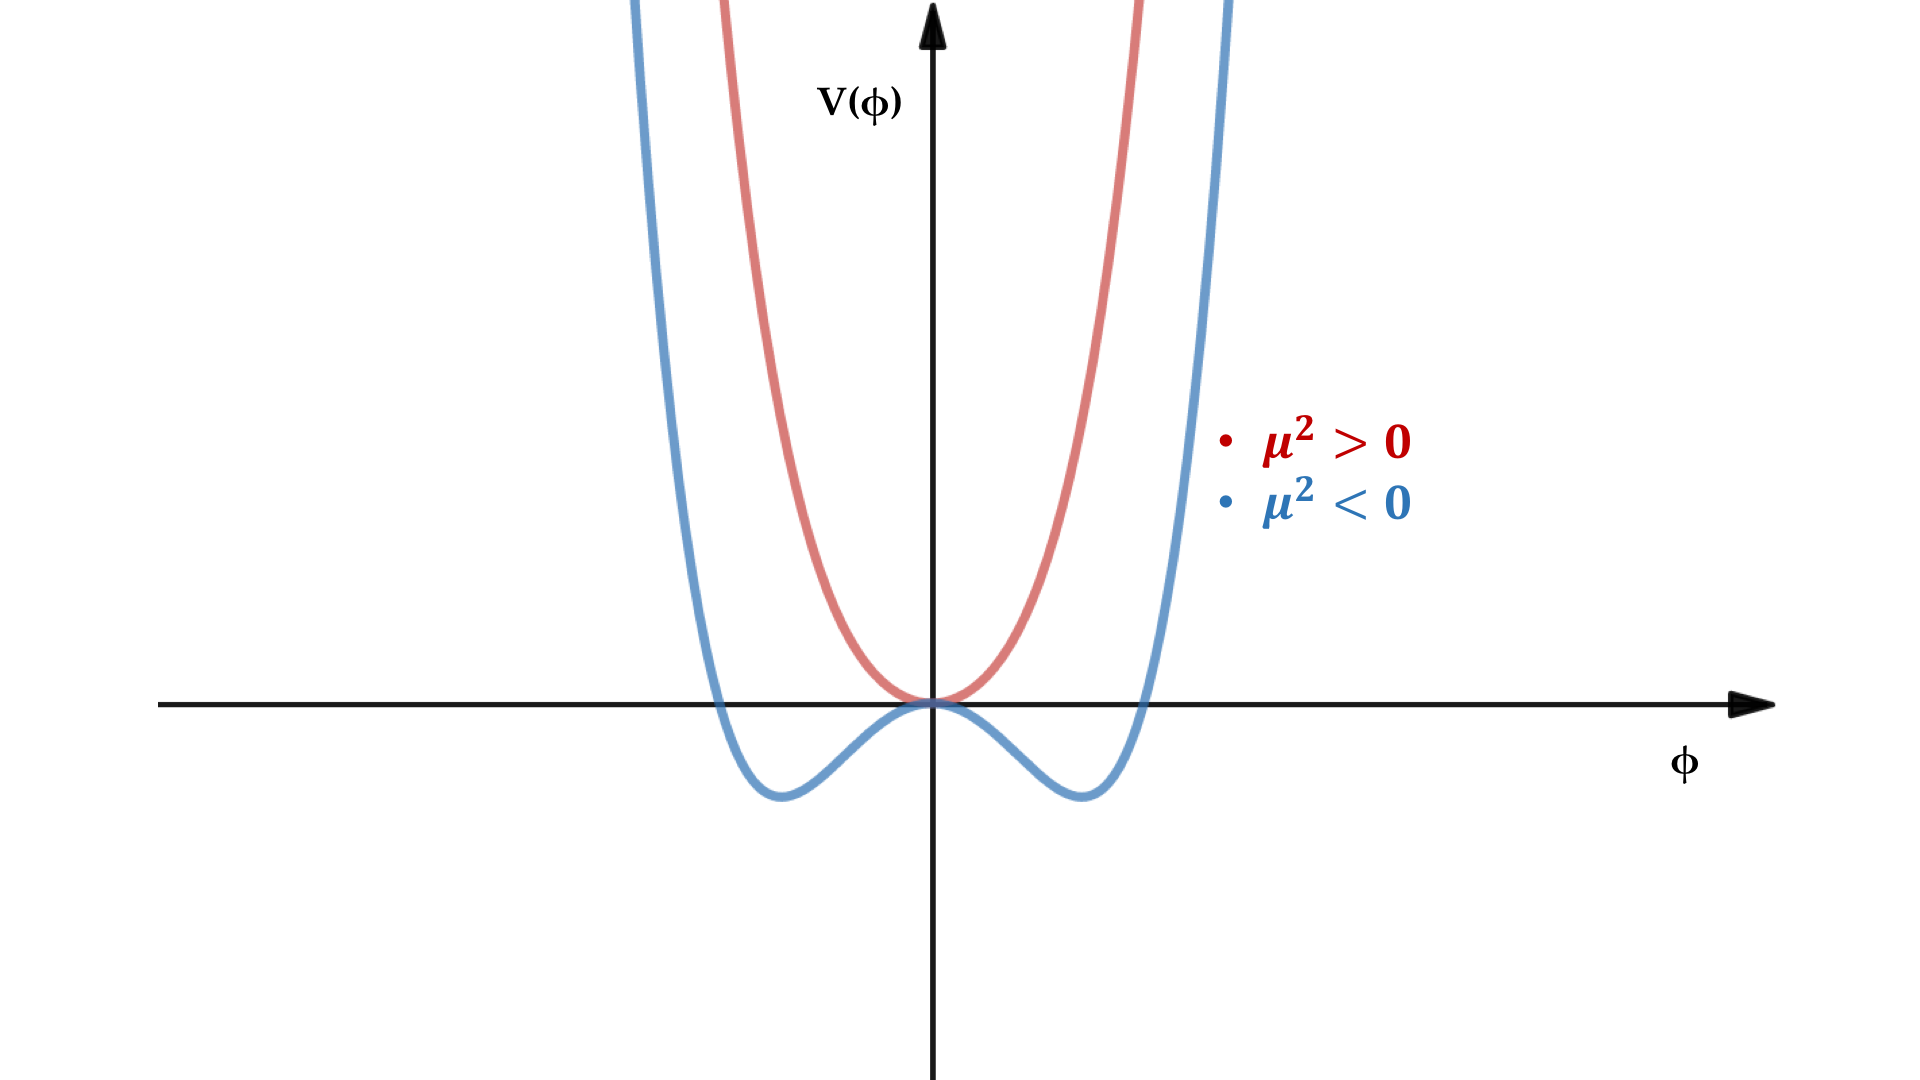
\includegraphics[width=\textwidth]{Theory/Higgs.png}
  \caption{Graphical representation of the potential $V(\phi) = \frac{1}{2}\mu^2\phi^2 + \frac{1}{4}\lambda\phi^4$ for both the $\mu^2<0$ (blue) and $\mu^2>0$ (red) scenarios (made using Ref.~\cite{desmos}). }
  \label{fig:higgs_potential}
\end{figure}

Taking the look at the first derivative in order to find the local extrema:

\begin{equation}
    \frac{\partial V}{\partial \phi} = \mu^2\phi + \lambda \phi^3 = 0,
\end{equation}

leads to the scenarios of $\phi_a = 0$ (for the $\frac{\partial^2 V}{\partial \phi^2} = \mu^2>0$) and $\phi_b = \pm|-\frac{\mu^2}{\lambda}|$ (for the $\frac{\partial^2 V}{\partial \phi^2} = -2\mu^2>0$ or the $\mu^2<0$ case). The symmetry breaking of the Lagrangian happens when a choice between the two values of $\phi_b$ are made (in further text renamed as $v = |\phi_b|$). Expressing $\phi$ in terms of its vacuum expectation state, one can introduce $H(x)$ and rewrite the Lagrangian as:
\begin{equation}
    \phi(x) = v+H(x),
\end{equation}
\begin{equation}
    \mathcal{L} = \frac{1}{2}(\partial_{\mu}H)(\partial^{\mu}H) - \frac{1}{2}\mu^2(v+H)^2 - \frac{1}{4}\lambda(v+H)^4.
\end{equation}

Grouping of terms quadratic in $H(x)$ leads to its mass term within the Lagrangian, or in other words: $m_{H} = \sqrt{-2\mu^2}$.

\hspace{10pt} A natural extension leads to the inclusion of a complex version of the aforementioned potential with $\phi = \frac{1}{2} (\phi_1+i\phi_2)$ and $V(\phi) = \mu^2\phi^*\phi+\lambda(\phi^*\phi)^2$. Repeating the search for global minimum leads to the possible choice of a vacuum state of $\phi_{vac} = (v, 0)$ and the re-composition of $\phi$ as: $\phi = \frac{1}{2}(v+H(x)+i\chi(x))$. As a second step in the process, a good way to evolve the simplified Lagrangian is to take a look at the U(1) gauge symmetry. This can be done by using the kinetic term with the appropriate re-definitions of the partial derivative (as done in Section~\ref{sec:ew_unification} for $B_{\mu}$) as well as using the choice of the unitary gauge in order to remove the $\chi$ dependency\footnote{This can be achieved by choosing $\lambda(x) = -\frac{1}{g^{'}v}\chi(x)$}. This new Lagrangian, when rewritten in terms of $H(x)$, yields a massive scalar field, the Higgs field, associated with $m_{H} =\sqrt{2v^2\lambda}$ alongside a massive gauge boson (associated with $B_{\mu}$) and the appropriate interaction and self interaction terms.

\hspace{10pt} Lastly, this approach is to be applied to the $SU(2)_L\times U(1)_Y$ symmetry group, as previously defined in Section~\ref{sec:ew_unification} closely associated with the unified electroweak interaction. This requires a re-definition of $\phi$ through a weak isospin doublet and the usage of the Lagrangian defined with Equation~\ref{eq:ew_unification}. Following the procedure of searching for a global minimum, applying the unitary gauge and expanding the Lagrangian in terms of $H(x)$ gives a similar, yet slightly more complex picture. Grouping the mass terms for the appropriate fields ultimately yields:
\begin{equation}
m_W=\frac{1}{2}g_Wv,~ m_Z = \frac{v}{2}\sqrt{g^{'2}+g_W^2}~\text{and}~m_A = 0\footnote{Where the latter two are obtained through the diagonalization of the mass matrix as explained in great detail in Ref.~\cite{thomson_2013}.}.
\end{equation}

\hspace{10pt} Before concluding this part of the story, there is one more topic that needs to be addressed and that is the mechanism through which fermions acquire their mass. In order to add an item corresponding to the mass term of fermions within the electroweak lagrangian, it has to be invariant under $SU(2)_L\times U(1)_Y$ transformations. For the $I_W^3 = -\frac{1}{2}$ fermions this term can be written as:

\begin{equation}
\mathcal{L} = -g_f(\overline{L}\phi R+ \overline{R}\phi^{\dagger}L),
\end{equation}

where $g_f$ denotes the Yukawa coupling and L (R) represents the SU(2) doublet (singlet). Through the process of spontaneous symmetry breaking, upon rewriting the Lagrangian in terms of $H(x)$, it can be seen that the fermion masses can be associated with the Yukawa coupling as:
\begin{equation}
    m_f = \frac{vg_f}{\sqrt{2}}
\end{equation}

\hspace{10pt} After the introduction to the SM presented here, the following chapter will connect the advancements made in collider physics with the potential for beyond the SM physics through the idea behind the invisible decays of the Higgs boson. 
%\chapter{Higgs Boson and collider experiments}
\chapter{When Higgs Boson met dark matter...}
\epigraph{\itshape``Nothing in life is to be feared, it is only to be understood. Now is the time to understand more, so that we may fear less."}{--- \textup{Marie Curie}}
\label{ch:Higgs_LHC_DM}
\section{Introduction}


\hspace{10pt}\lettrine[lines=2]{\initfamily{B}}{eing the main focus} for studies covered by this thesis, special attention needs to be given to the Vector Boson Fusion production mode of the Higgs boson, while also discussing other topologies interesting for the invisible final state. Upon completing this discussion, a slight turn in focus is going to be taken in order to introduce the current understanding of the term dark matter. It is presented alongside the investigation of a possible connection between dark matter searches and measurements of properties of the Higgs boson performed at hadron collider experiments. This will culminate with the illustration of the analysis idea for probing of the SM through the invisible final state of the Higgs boson decay. Finally, in order to complete the whole picture, the statistical apparatus used with this approach is discussed, alongside a brief overview of previously obtained results.


\section{Production modes of the Higgs boson}
\label{sec:prod_higgs}
\hspace{10pt} The main interest of the two general purpose experiments centered around the interaction points of the Large Hardon Collider~\cite{LHC_TDR} (consequently for this thesis as well) is the production and subsequent decays of the Higgs boson. Figure~\ref{fig:higgs_prod_diag} shows diagrams for its various production mechanisms relevant for hadron colliders, in this case the proton-proton collisions (more details about the experimental setup are given in Chapter~\ref{ch:cms_experiment}).

\begin{figure}[htbp]
    \begin{center}
        \subfigure[$ggH$]{
        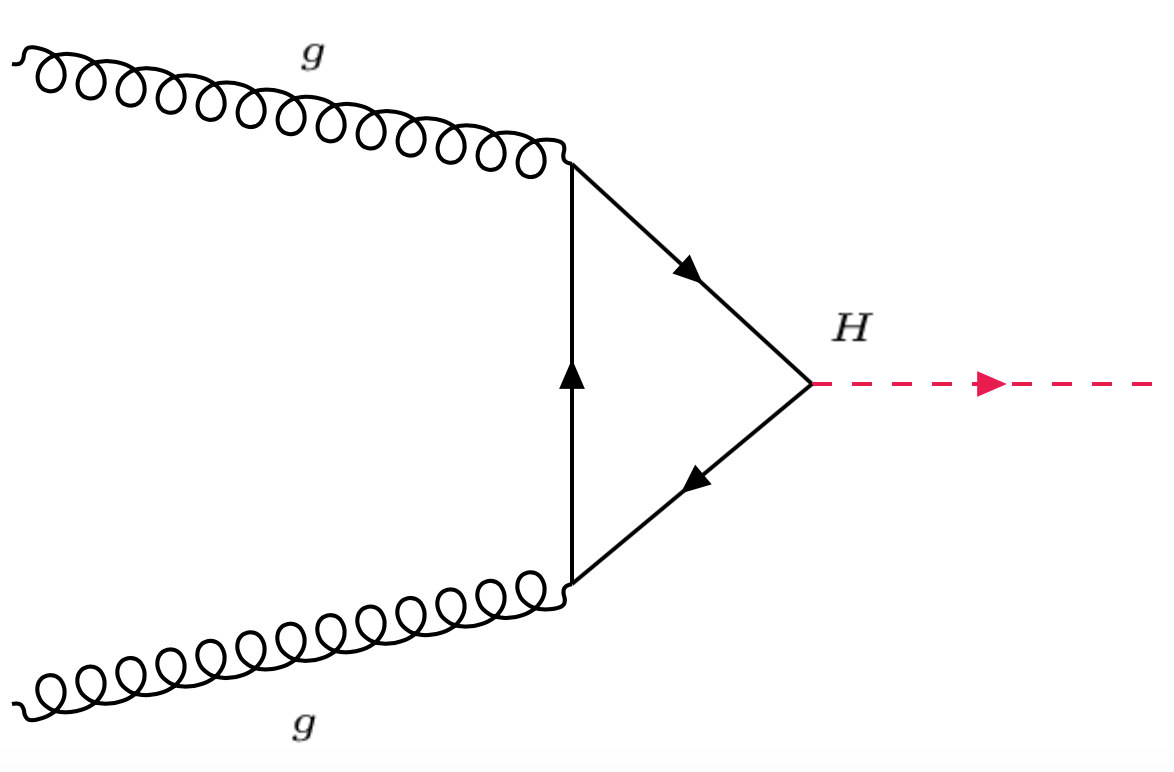
\includegraphics[width=0.45\textwidth]{Theory/ggH.png}}
        \subfigure[$qqH$]{
        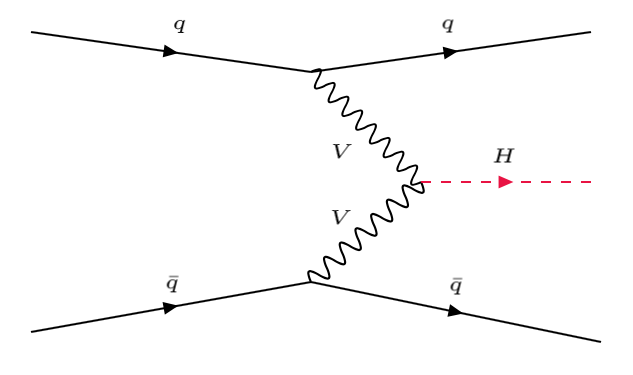
\includegraphics[width=0.45\textwidth]{Theory/vbf.png}}\\
        \subfigure[$VH$]{
        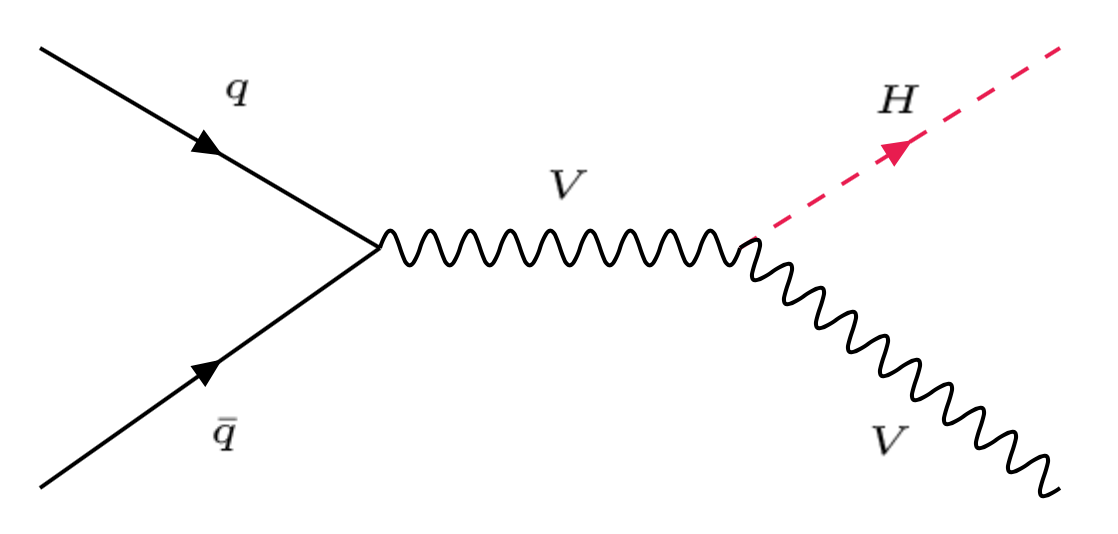
\includegraphics[width=0.45\textwidth]{Theory/VH.png}}
        \subfigure[$ttH$]{
        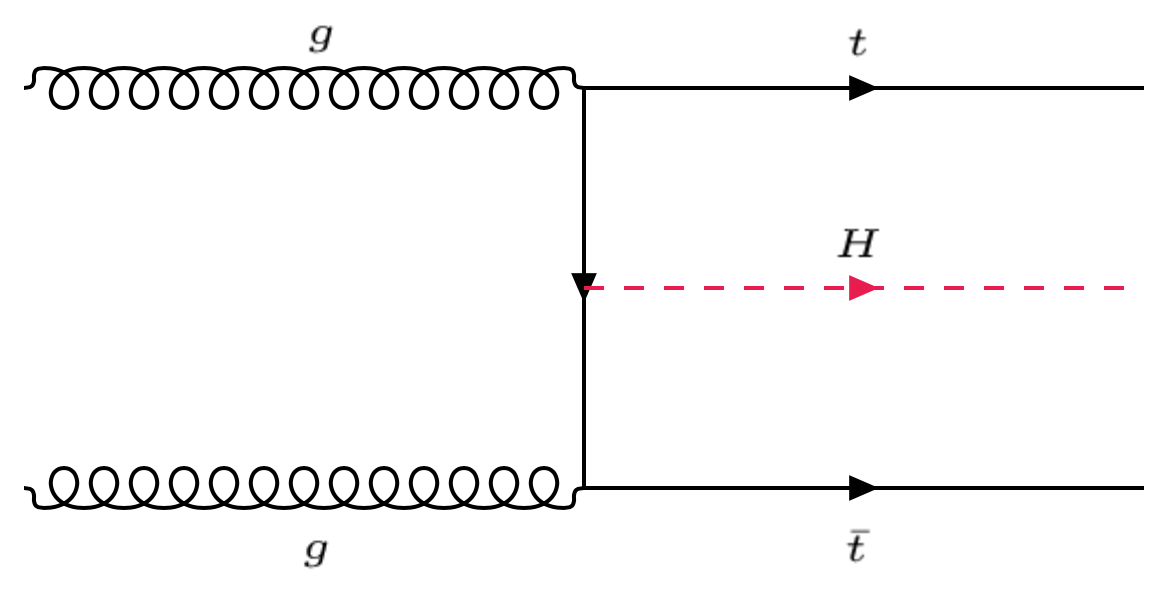
\includegraphics[width=0.45\textwidth]{Theory/ttH.png}}    
        \caption{Diagrams for the main production mechanisms of the Higgs boson: a) gluon gluon fusion, b) vector boson fusion, c) Higgs-strahlung and d) associated production with top quarks (diagrams were made using Ref.~\cite{fey_diag}).}
      \label{fig:higgs_prod_diag}
    \end{center}
  \end{figure}

\hspace{10pt} The production mode with the largest cross section is the gluon-gluon fusion (ggH)~\cite{paper:ggH1,paper:ggH2}, where jets\footnote{A collimated stream of hadrons.} can arise due to initial state radiation (ISR)\footnote{Leading to a reduction of the production cross section (subsequently its importance), but still being relevant to these studies.}. The production of a Higgs boson proceeds through, as the name suggests, a gluon fusion forming a virtual quark loop which ultimately yields the aforementioned boson. The production mode with the second largest cross section, but the highest importance for this thesis, is the vector boson fusion (qqH or simply VBF) mechanism~\cite{paper:ggH1,paper:ggH2,paper:vbf1,paper:vbf2}. The collision enables an exchange of virtual vector bosons which fuse together to produce a Higgs boson. Its distinct signature includes a large geometrical separation of the jets and a large dijet invariant mass.

\hspace{10pt} The Higgs strahlung or the associated VH production~\cite{paper:vh} happens when the colliding particles produce a virtual vector boson which can emit a Higgs boson. Lastly, a Higgs boson can be produced in association with top quarks~\cite{paper:tth1,paper:tth2}. Figure~\ref{fig:hig_production_xs} shows the production cross sections for these scenarios ranging over various proposed masses of the Higgs boson, serving as an illustrative example of the order of importance for the SM Higgs boson.

\begin{figure}[htbp]
    \begin{center}
        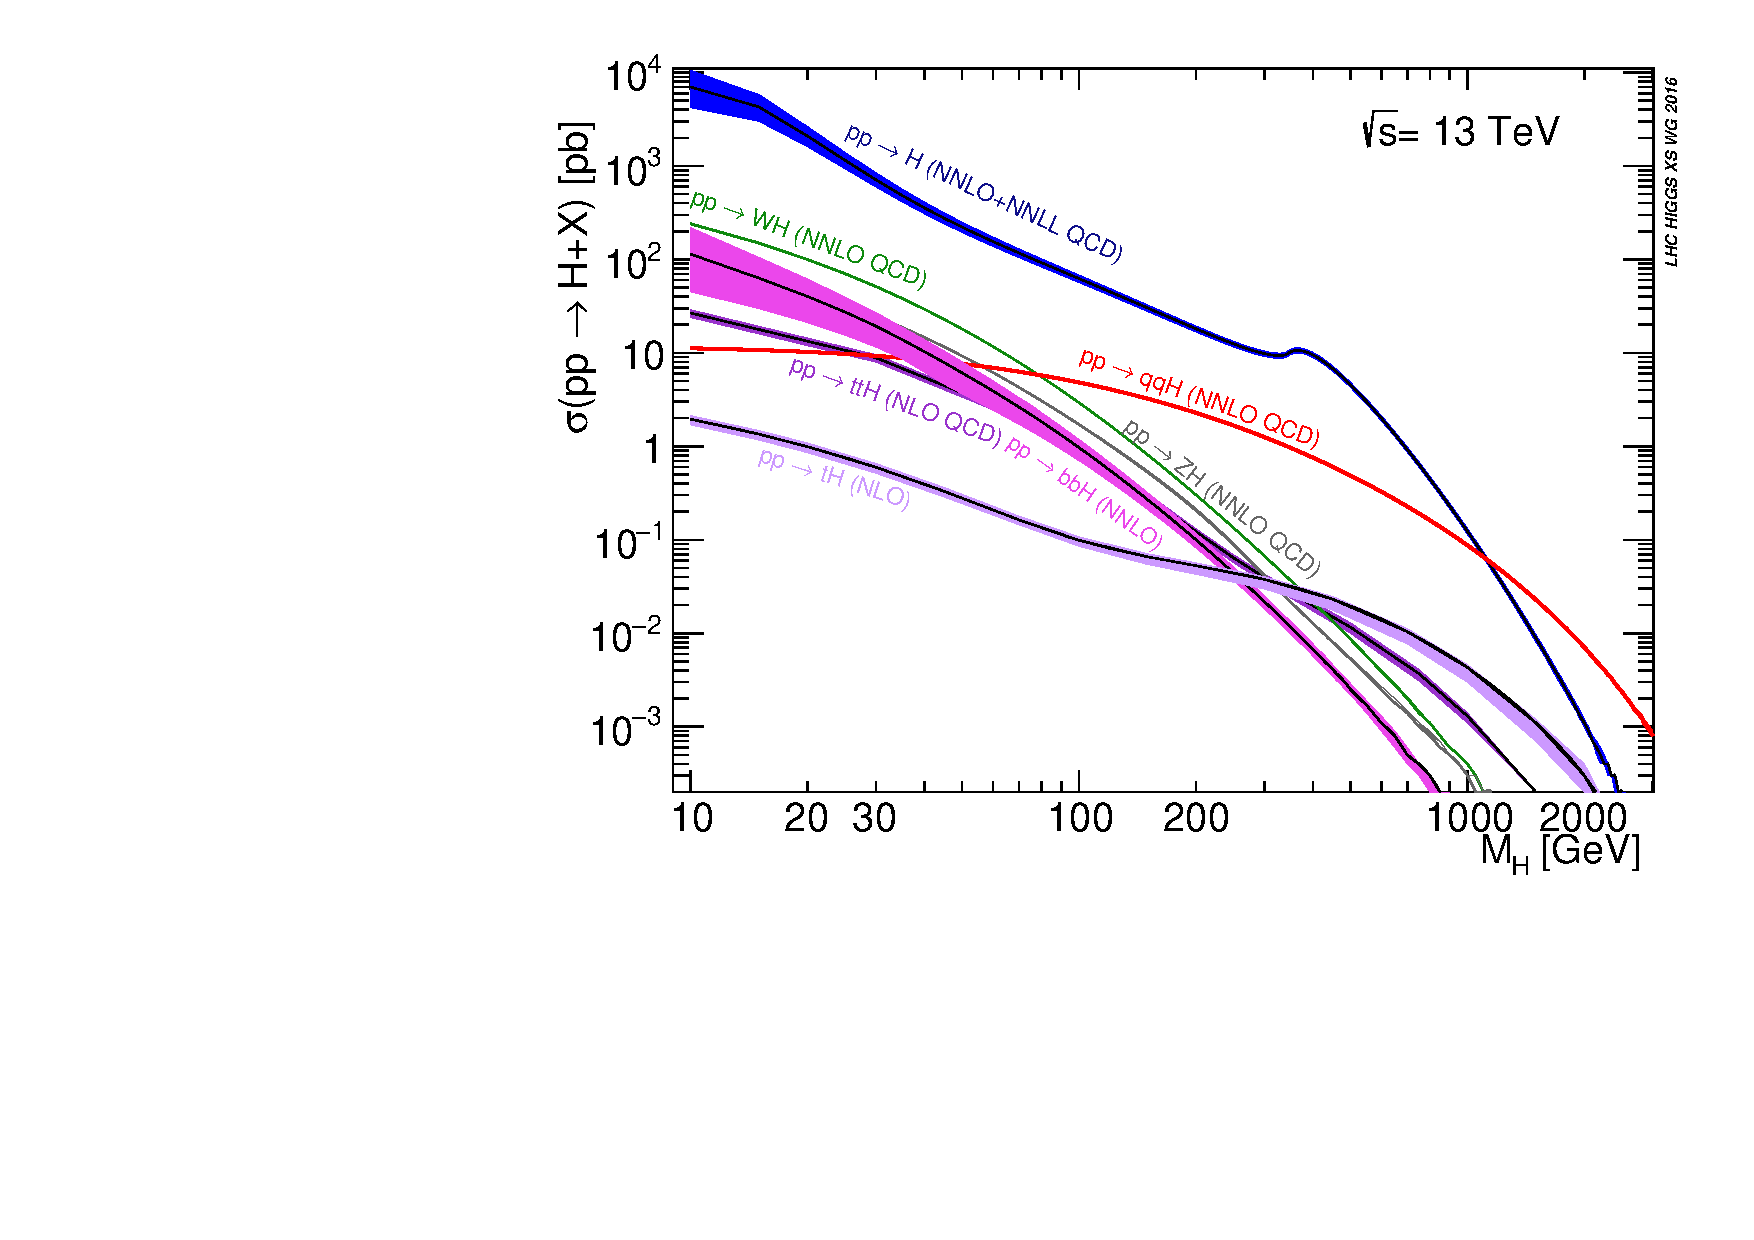
\includegraphics[width=0.88\textwidth]{Theory/higgs_prod_13TeV.pdf}  
        \caption{Cross sections for various production mechanisms of the Higgs boson originating from proton-proton collisions at the energies of $\sqrt{s}=$~13~TeV~\cite{twiki:lhcxswg}.}
      \label{fig:hig_production_xs}
    \end{center}
  \end{figure}

\hspace{10pt} The measurements of properties of the Higgs boson, which followed its discovery by the Large Hadron Collider experiments~\cite{paper:higgs_discovery1,paper:higgs_discovery2}, show a good agreement with the SM~\cite{paper:higgs_prop1,paper:higgs_prop2,paper:higgs_prop3}, but the uncertainties on these measurement are not yet small enough to fully exclude the possibility of physics beyond the SM. The current generation of collider experiments is not able to reach the O(MeV) range of precision needed to test the $\Gamma_{SM}^H$ (the total decay width of the Higgs boson predicted by the SM), leaving an indirect way of testing for beyond the SM physics\footnote{Within the area of physics concerned with Higgs boson decays} with only one other option - to make use of results arising from measurements of the visible final states in order to set an upper limit on the beyond the SM branching ratio. This has lead to the aforementioned result where this approach yields an 95\% Confidence Level (CL) upper limit on the branching ratio of the Hiigs boson to invisible final state\footnote{More details about this approach, alongisde with a detailed introduction to the $\kappa$ framework is given in Ref.~\cite{report_lhcxswg_3}} of Br(H$\rightarrow$inv)$~\sim$~0.34~\cite{paper:higgs_prop1}, thus motivating a more direct approach.

% Figure~[R] further expands on this discussion showing the results of combined measurements from CMS and ATLAS collaborations expressed in terms of the coupling factors $\kappa_X$ (the corresponding model being introduced in Ref.~[R]), where the $k =$ 1 denotes agreement with the SM\footnote{The $\kappa_X$ facttors are intrdoced as additional multipliers to the coupling constants of the Higgs to the respective particles found in the final state. When the value of $\kappa_X=$~1 it states that no modification of the SM predicted coupling constant is needed.}


\section{Invisible final state}
\hspace{10pt} The interest surrounding final states involving particles invisible to hadron collider detectors is due to the potential BSM physics hiding within their cloak. From the perspective of studies involving the Higgs boson properties, the SM predicts that the fully invisible decay is highly suppressed with Br(H$\rightarrow4\nu$)$\sim$~0.1\%~\cite{report_lhcxswg_3}, making it a good option for testing for BSM physics. As mentioned in the previous section, the limiting factors arising from the indirect searches create motivation for this, more direct, approach~\cite{paper:hinv_run1,paper:HIG_17_023,Patrick,Riccardo}. Connection to dark matter (DM) searches can be found in Higgs portal theories~\cite{paper:hig_portal_models1,paper:hig_portal_models2,paper:hig_portal_models3,paper:hig_portal_models4}, where the Higgs boson can take the role of a mediator between the particles from two sectors (SM and DM), but more about those in the following section. In order to be able to approach this invisible final state with current detectors, the Higgs boson is required to recoil against a visible system.

\hspace{10pt} The production mode bringing the most sensitivity to this final state is the VBF where, as introduced in Section~\ref{sec:prod_higgs}, the Higgs boson is associated with two jets. From the SM side, there are a few processes which can mimic the exact final state of interest and those are mostly originating from V+jets processes (where V denotes W or a Z boson). Their contribution can be categorised into reducible or irreducible. The completely irreducible scenario is found when the Z boson decays to two neutrinos (the Z~$\rightarrow\nu\nu$ decay) and for the W$~\rightarrow l\nu$ case (where the charged lepton has been missed in the detection process). Example diagrams showing both the strong and electroweak modes of production (in further text reffered to as QCD and EWK modes) of a Z boson decaying to neutrinos are shown in Figure~\ref{fig:znunu_diagram}. 

\begin{figure}[htbp]
    \begin{center}
        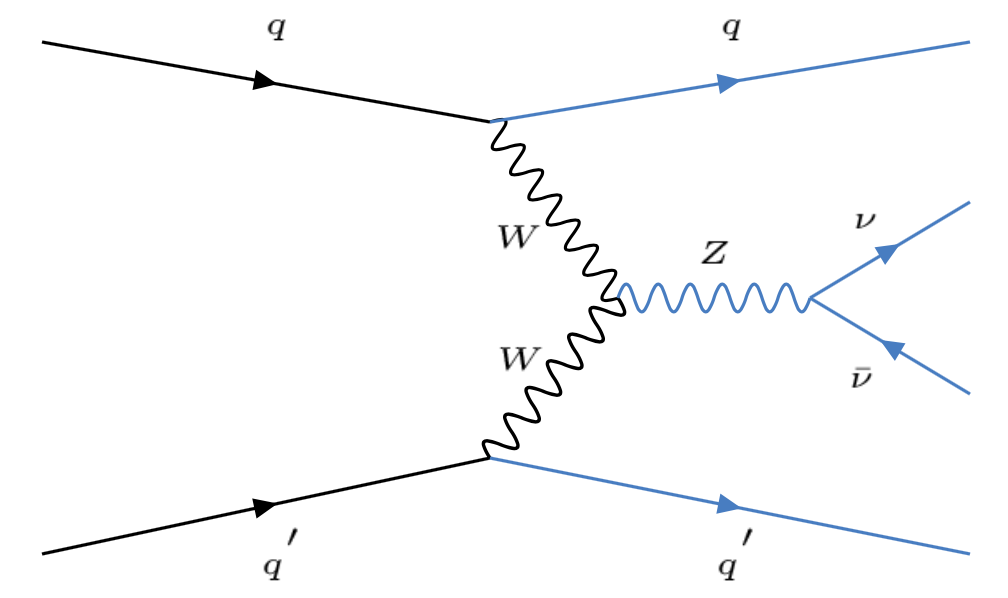
\includegraphics[width=0.47\textwidth]{Theory/ewk_znunu.png}
        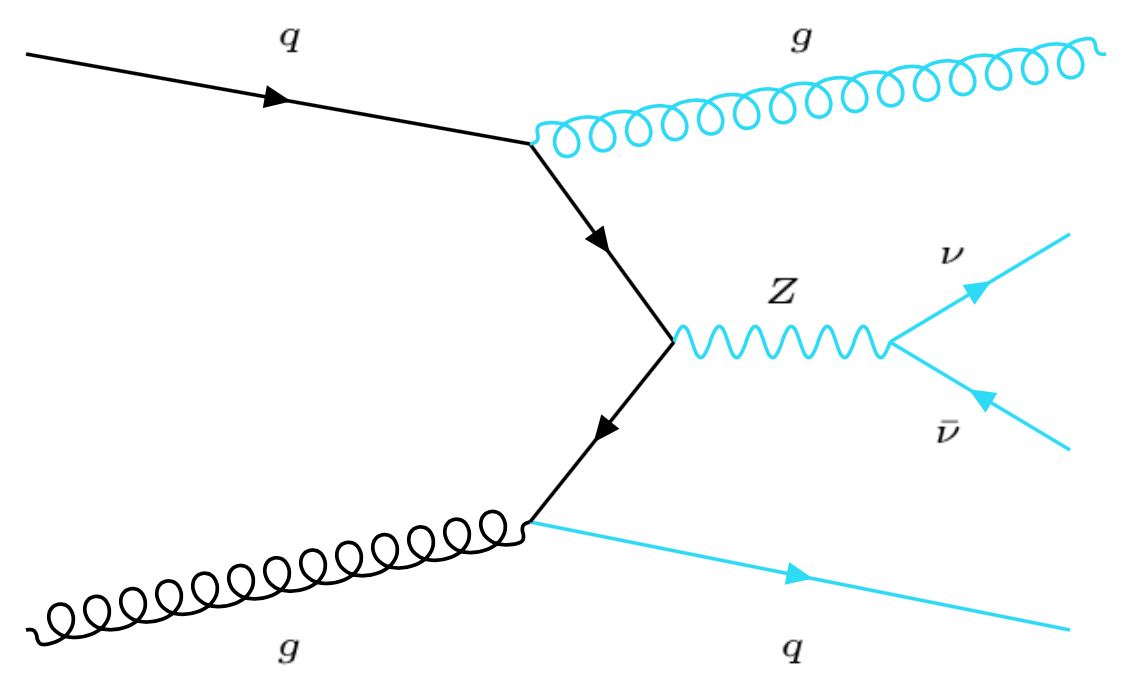
\includegraphics[width=0.47\textwidth]{Theory/qcd_znunu.png}
        \caption{Feynman diagrams for two main $Z\rightarrow \nu\nu$ irreducible background SM processes shown for both the EWK (left) and QCD (right) production modes at leading order (colors assigned to final states follow the choice used to mark the corresponding processes in further chapters). The diagrams were made using Ref.~\cite{fey_diag}.}
      \label{fig:znunu_diagram}
    \end{center}
  \end{figure}


\hspace{10pt} An additional background contribution can arise from strong multijet processes, which due to their large production rate can produce a sizeable contribution which mimics the desired final state. The estimation of the contribution originating from these main irreducible background processes is the focus of Chapter~\ref{ch:control_regions} where data driven methods are deployed. Additional minor contributions, which can arise from diboson (VV) and top quark ($t\overline{t}$ and single top) processes, are estimated through the use of simulated samples of respective processes.

\section{The dark connection}
\label{sec:dm}
\hspace{10pt} With all the great knowledge regarding particle physics currently written down as the SM, it still does not account for all of the matter in the universe. Many cosmological observations suggest that there exists another form of matter which does not posses an affinity towards the electromagnetic interaction - dark matter~\cite{intro_dm}. Following the current cosmological model, it is categorised that $\sim$~5\% of the universe's mass-energy is visible matter, 27~\% dark matter and 68\% dark energy~\cite{paper:dm_composition}.

\hspace{10pt} The most commonly used observation illustrating this is the appearance of a discrepancy in the distributions of rotation velocities of spiral galaxies when comparing the predicted result (which assumes they are comprised only from visible matter) to what is observed in reality. This is illustrated in Figure~\ref{fig:DM}, where the observed velocity distribution $V_C(Radius)$ (with its corresponding fit), represented with points (solid line), is compared with the visible matter only approach (dashed lines denoting disk and gas contribution) alongside a DM halo contribution (dashed line with the point) accounting for the missing piece~\cite{paper:dm_vc}. This can be expanded with a list of other studies as the ones focusing on galaxy clusers~\cite{paper:dm_gal_clust} and gravitational lensing~\cite{paper:dm_grav_lens}.

\begin{figure}[htbp]
    \begin{center}
        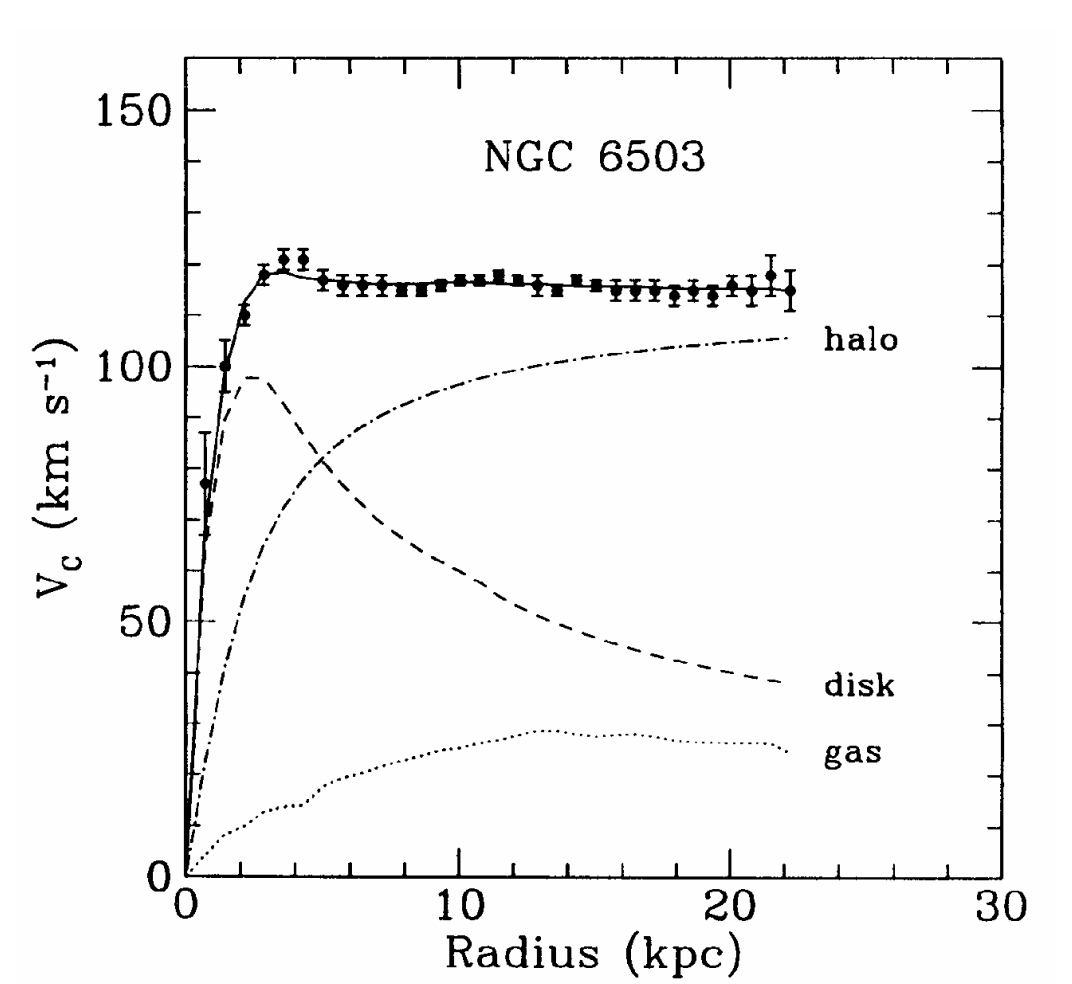
\includegraphics[width=0.7\textwidth]{Theory/DM_velocity.png}
        \caption{The distribution of the rotation velocity for the NGC 6503 is presented as an example of cosmological observation of DM~\cite{paper:dm_vc}.}
      \label{fig:DM} 
    \end{center}
  \end{figure}



\hspace{10pt} Staying in the area relevant to the theme of this thesis, the potential candidates for particles comprising the invisible final state discussed above can be associated with the DM sector. This would require a modification of the SM Lagrangian to include terms which enable the coupling of the Higgs boson to the particles from the DM sector. These can include one of the following scenarios~\cite{paper:hinv_run1, paper:hig_portal_models1,yellow_report}:
\begin{equation}
    \mathcal{L}_{S} = -\frac{1}{4}g_{HSS}H^\dagger H S^2,~\mathcal{L}_{V} = \frac{1}{4}g_{HVV}H^\dagger HV_\mu^\dagger V^\mu~\text{and}~\mathcal{L}_{f} = \frac{1}{4}g_{H\chi\chi}H^\dagger H\overline{\chi}\chi
\end{equation}
where $\mathcal{L}_{S}$ shows the (quartic) interaction term connecting the SM Higgs doublet with the DM sector, this time being represented with a scalar type (S). The equivalent definitions stands for the latter two terms with the scalar DM field being replaced with a vector and a fermion type, respectively.

%\hspace{10pt} The following sections introduce the statistical approach taken in order to estimate the upper limit on the H$\rightarrow$inv branching ratio, representing a necessary step needed before continuing to explore this DM-invisible final state connection.


%\section{The CLs approach}

%\hspace{10pt} The characteristics of the VBF topology are manifested through the existence of two jets. Through an optimisation technique it was shown that the largest signal versus background shape separation is gained when deploying the dijet invariant mass as the main analysis tool\footnote{More details about the jet properties from the perspective of the VBF production mode are given in Chapter~\ref{ch:an_strategy}.}~\cite{paper:HIG_17_023,Riccardo}. For a measurement of the aforemnetioned property, the resulting data can be represented with a binned histogram (with $d_i$ denoting a certain mass bin). Due to the nature of collider experiments, the use of Poisson statistics is applicable to studies of this kind. This allows for the introduction of the binned likelihood function as:
%\begin{equation}
%    \mathcal{L}(\mu, \boldsymbol{\theta}) = \prod_i \frac{(\mu S_i(\boldsymbol{\theta})+B_i(\boldsymbol{\theta}))^{d_i}e^{-(\mu S_i(\boldsymbol{\theta})+B_i(\boldsymbol{\theta}))}}{d_i!} = \prod_i Pois(d_i|(\mu S_i(\boldsymbol{\theta})+B_i(\boldsymbol{\theta})),
%\end{equation}
%where the terms comprising the product can be interpreted as the probabilities that $d_i$ occurences of the dijet mass confined to the bin range of $i$ has been observed given the expected valued of events being $\mu S_i(\boldsymbol{\theta})+B_i(\boldsymbol{\theta})$~\cite{paper:stat_overview,paper:cls_intro}. The bin values associated to the signal ($S_i(\boldsymbol{\theta})$) and background ($B_i(\boldsymbol{\theta})$ processes are obtained from the simulation of SM processes and the dependency on a set of nuisance parameters $\boldsymbol{\theta}$. Lastly, the $\mu$  is also free parameter in the fit and in this scenario it represents the desired branching ratio. The test statistics can now be formed as: $q_\mu = -2ln\frac{\mathcal{L}(\mu, \boldsymbol{\theta(\mu)})}{\mathcal{L}(\mu_m, \boldsymbol{\theta_m})}$, where $\mu_m$ and $\theta_m$ represent the values of the parameters yielding the largest value of the Likelihood funcion, and $\theta(\mu)$ denotes the value of a parameter $\theta$ which maximises the Likelihood function for a given choice of $\mu$. 

%\hspace{10pt} When approaching a task of setting a limit on the probability of the Higgs boson decaying invisibly, one must propose a way of thinking opposite to the case when there is a hunt for a discovery. In these scenarios, In these scenarios, the null hypothesis ($H_0$) is represented by the signal~$+$~background scenario which is compared to the alternative ($H_1$) denoted as background only scenario (as introduced in Ref.~\cite{paper:stat_overview}). For the purposes of the VBF H$\rightarrow$inv search that would introduce the options of including the SM Higgs by fixing the values of Br(H$\rightarrow$inv) to be 1 or 0 respectively. Following from the previous definitions, the final comparison can be made by following the CLs criterion~\cite{paper:stat_overview,paper:cls_intro}, through which the value of the 95\% CL upper limit on Br(H$\rightarrow$~inv) is obtained.

%\hspace{10pt} This simplified method of having only one region represented with $\mu S_i+B_i$ is used to illustrate the entire process without the pressure of multiple additional background enriched regions. Those are going to be the focus of later chapters (\ref{ch:an_strategy} and~\ref{ch:control_regions} to be precise), while the details of their inclusion into the signal extraction procedure are given in Chapter~\ref{ch:fit}.

%(large number of event accompanied by a small proability for an intersting event to occur)
\section{Current status}
\hspace{10pt} The most recent publication on this matter related to the CMS experiment represents a combination of efforts from both the entire Run 1 and early Run 2 phase of operation of the Large Hadron Collider\footnote{More details on the different phases are given in Chapter~\ref{ch:cms_experiment}}~\cite{paper:HIG_17_023}. It yields a value of the 95\% CL upper limit on the branching ratio for the invisible final state of Br(H$\rightarrow$~inv) = 0.19 (0.15) for the observed (expected) scenario, through the combination of various analyses targeting different production mechanisms of the Higgs boson. Figure~\ref{fig:limit_2016} shows the 95\% CL upper limits on the Br$(\text{H}~\rightarrow \text{inv})$ with respect to each production mode of interest (denoted as tag, eg. VBF-tag) for the 2016 era of data taking (representing the early stage of Run 2). The additional tags, besides the already discussed VBF, focus on the VH production, which is split into two separate tags depending on the decay of the vector boson being fully leptonic (Z$\rightarrow$ll) or hadronic (V$\rightarrow$qq), and the ggH produciton (with the requirement of having one jet from ISR associated with it).


\begin{figure}[htbp]
    \begin{center}
        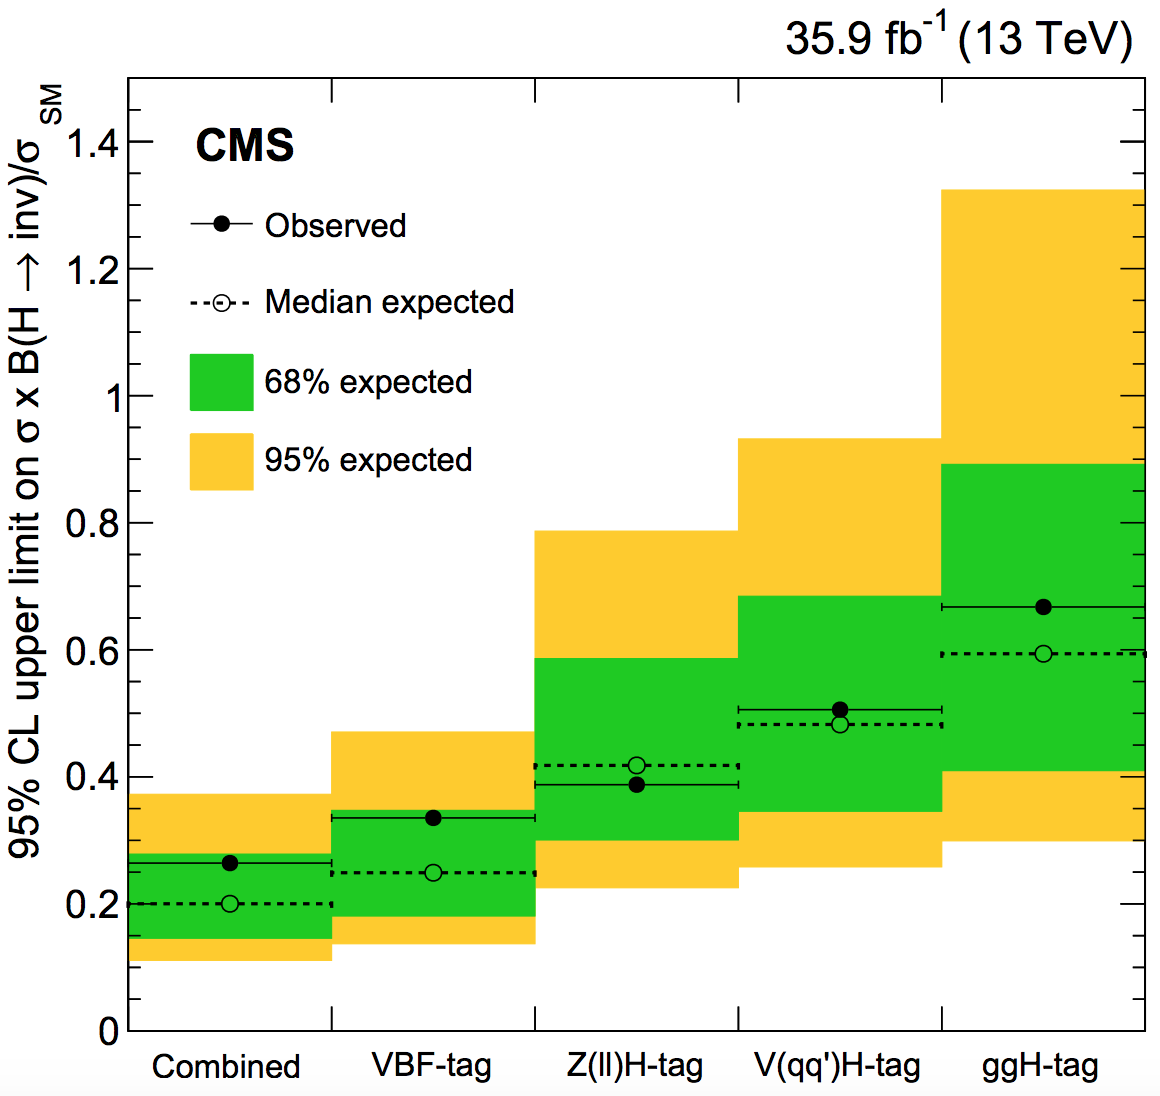
\includegraphics[width=0.7\textwidth]{Theory/Limit2016.png}
        \caption{Summary of results from the CMS experiment for the 95\% CL upper limit on the $\sigma \times$~Br(H$\rightarrow$~inv)$/\sigma_{SM}$ under the assumption of the SM Higgs boson, for the 2016 era of data taking.~\cite{paper:HIG_17_023}.}
      \label{fig:limit_2016}
    \end{center}
  \end{figure}
\hspace{10pt} Continuing the story which began in Section~\ref{sec:dm}, these results can be interpreted in terms of the upper limit on the spin-independent DM-nucleon interaction cross section making it easier to compare with direct detection experiments. The conversion can be made using the following relations (with the assumption of a scalar or a fermion DM particle respectively)~\cite{paper:hinv_run1,paper:hig_portal_models1}:

\begin{equation}
    \mathcal{B}(\text{H}\rightarrow \text{inv}) = \frac{\Gamma_{inv}}{\Gamma_{SM}+\Gamma_{inv}}
\end{equation}
\begin{equation}
    \sigma^{SI}_{Scalar-N} = \frac{4\Gamma_{inv}}{\beta m^3_Hv^2}\frac{f_N^2m_N^4}{(m_N+m_{DM})^2},
\end{equation}
\begin{equation}
    \sigma^{SI}_{Fermion-N} = \frac{8\Gamma_{inv}m_{DM}^2}{\beta^3m^5_Hv^2}\frac{f_N^2m_N^4}{(m_N+m_{DM})^2},
\end{equation}

where the values of the parameters are: $m_N = 0.939$~GeV (average mass of the proton and neutron), v = 246~GeV, the DM candidate's mass ($m_{DM}$), $\beta = \sqrt{1-\frac{4m_{m_{DM}}^2}{m_H^2}}$, and the $f_N=0.308$ (nuclear form-factor~\cite{paper:form_fact, paper:HIG_17_023}). Figure~\ref{fig:dm_2016} shows the comparison of the CMS experiment's results compared to results coming from direct detection experiments. These show that the approach taken by this analysis, covering $m_{DM}<\frac{m_H}{2}$, leads to a set of results complementing the majority of direct detection experiments. %avoiding the competition aspect while enhancing the affinity towards cooperation in order to achieve a better look at the overall picture.
\newpages
\hspace{10pt} This chapter concludes the first part of this thesis which served as an introduction to main mechanisms of the SM and the motivation driving the search for the invisible final state of the Higgs boson. The following chapters introduce the experimental setup - the CMS experiment. There it will be presented how these measurements are made possible on the detector and trigger level. The continuation of this idea from the perspective of the newly available data is the focus of Chapter~\ref{ch:an_strategy} and beyond, where a combination of new trigger ideas and improved analysis strategy is discussed in great detail.

  \begin{figure}[htbp]
    \begin{center}
        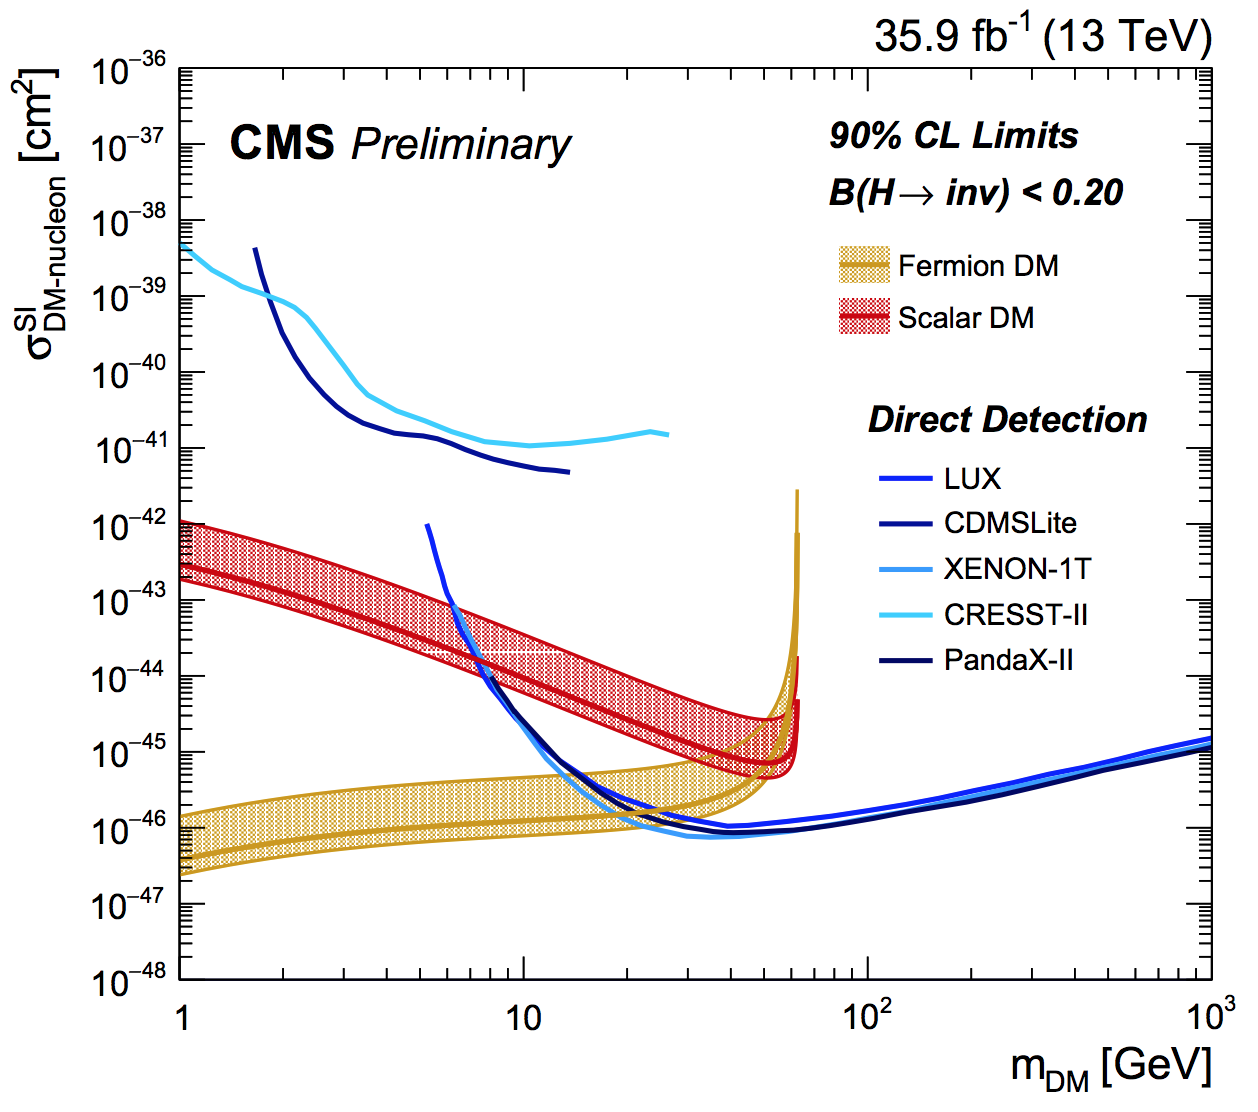
\includegraphics[width=0.75\textwidth]{Theory/DM2016.png}
        \caption{The reinterpretation of the CMS results in terms of the 90\% CL upper limits on the spin-idependent DM-nulcleon scattering cross section when assuming a fermion (red) or a scalar (orange) DM particle (presented as a function of $m_{DM}$). Limits are compared with results originating from direct detection DM experiments.~\cite{paper:HIG_17_023}.}
      \label{fig:dm_2016}
    \end{center}
  \end{figure}


\newpage
 \newgeometry{left=0cm,bottom=0cm,top=0cm,right=0cm}
  \begin{tikzpicture}[remember picture, overlay]
  \node[inner sep=6pt] (chapter) at (current page.center){\Huge Part II: The experiment};
  \node[inner sep=12pt, below of=chapter, text width=10cm, align=center, outer sep=12pt] (title1) {\large \textit{``Bez alata nema zanata."}};
  \node[inner sep=12pt, below of=title1, text width=10cm, align=center, outer sep=12pt] (title) {-- \textup{Serbian proverb} --};
  \node[anchor=north] at (title.south){\pgfornament[width=5cm]{87}};
  \node[anchor=south] at (chapter.north){\pgfornament[width=4cm,symmetry=h]{58}};
  \end{tikzpicture} 
   \addcontentsline{toc}{part}{Part II: The Experiment}
 \restoregeometry
\newpage




\chapter{The LHC and the CMS experiment}
%\epigraphfontsize{\small\itshape}
\epigraph{\itshape``You cannot swim for new horizons until you have courage to lose sight of the shore."}{--- \textup{William Faulkner}}


\label{ch:cms_experiment}
\section{Introduction}
\subsection{A new dawn}

\hspace{10pt}\lettrine[lines=2]{\initfamily{T}}{ he European Organization for Nuclear Research}, better known by its abbreviation "CERN", stands tall as a pillar of the human determination towards understanding nature. Paving the way for future collaborations by being one of the first examples of unity after the horrors of the past decade, CERN has been a home to experts coming from a multitude of fields ever since it opened its doors on the 29th of September 1954~\cite{History_CERN_1}. 

\hspace{10pt} Carefully positioned near Geneva (Switzerland), the newly formed institute had its eyes set on becoming the world's leading research facility for high energy physics. The following sections are going to briefly summarize the overall achievements of this collaboration which lead to the fulfilment of this goal and explain how bold decisions have resulted in the state of the art experiments operating at the moment. The easiest way to describe it would be to categorize the main benefits of CERN into three groups: scientific results, industry application and education.

 \hspace{10pt} Starting with the scientific achievements, the discovery of weak neutral currents~\cite{neutral_currents_1}\cite{neutral_currents_2} in 1973 made a huge breakthrough by confirming one of the basic ideas of the SM. Fast forward to ten years later when, after building from the previously gained experience, a new ground breaking result had been reported from CERN's experiments. It was the experimental evidence of the existence of W and Z bosons~\cite{WandZ_discovery}. Further technological advances combined with a non-conventional scientific strategy led to the design and the creation of the Large Electron-Positron (LEP) collider~\cite{LEP_TDR}. What followed was a series of high profile results, some of which will be discussed in the next section, that culminated with the creation of the Large Hadron Collider (LHC) and the subsequent discovery of the Higgs boson by the CMS and ATLAS experiments in 2012.

\hspace{10pt}Looking at the aforementioned discoveries one could naively assume that, while they represent a giant leap in our understanding of nature, nothing coming out of CERN's doors has a direct impact on everyday life. Yet this couldn't be further from the truth. It can easily be seen by looking at something that is today considered an essential tool in lives of many, the World Wide Web standard. Born in the dark corridors of building 1 within the research campus of CERN, the basis of our digital life had been created by Tim Berners-Lee~\cite{www_origins} in the early 90s for the purpose of easier data management within the experiments. This standard introduced the concept of associating Universal Resource Locators (URLs) to documents and other objects of interest as means of identifying and accessing them via internet. After being used internally for two years, it was concluded that the possible applications far exceeded its original goal and thus it was released to the public, setting a basis for what we now call web browsing.

\hspace{10pt}This general concern about the practicality of published results plagues not only high energy physics but also many of the fundamental branches of science. This constant questioning is even more baffling due to the fact that if only a minuscule investigative effort was made by those who present such claims, then it would be clear that many of technological leaps were enabled through fundamental research. Moving from the real of the internet, additional examples of this can also be found in medicine where the contribution of accelerator sciences are ranging from hadron therapies, which provide a less invasive way of treating cancer cells, to the development of super absorbent polymers for the purpose of creating thin but still multi layered baby diapers. As it would be touched on in the following sections, there are also going to be further industry applications of standards developed for the purposes of CERN experiments (but more about that in Section~\ref{sec:data_acquisition}).

\hspace{10pt} Finally, there is one additional way in which CERN impacts our society as a whole and that is through its education platform. Its main purpose is to give new generations of students the opportunity to participate in various programs that range form high school projects to undergraduate internship positions. This approach has influenced a large number of young people from all over the world to get involved in this field from a fairly early age. Case in point, the author of this thesis began his journey into the field of particle physics with his high school graduation thesis by looking into a set of simulation samples for a four muon decay of the, then still theorised, Higgs boson. Even though it was a fairly simple project, it was still a harbinger of a, hopefully long, future research career.

\subsection{Down the road less travelled}
\hspace{10pt} As a good rule of thumb, the high energy physics (HEP) scientific community organizes meetings and workshops every few years in order to encourage the discussion regarding future experiments. This should come as no surprise as planning ahead and trying to see the bigger picture represent actions closely associated with almost every successful long term venture. The need for this approach became more evident in the decade that saw the experimental confirmation of the existence of the neutral current and the discovery of W and Z boson, as it became clear that there is an urgency for a structure that could probe the, then freshly finalized, Standard Model.

\hspace{10pt} The decision to move away from proton-antiproton machines, for which CERN had developed expertise in the past decade, in favour of an electron positron design had a much bigger impact on the institute (and HEP community as a whole) than it was initially envisioned. From a strictly physics point of view, this opened the door to a much cleaner slate that enabled detailed probing of the electroweak sector. On the other hand, taking a look at the engineering and monetary side, a circular collider being built under Geneva had pretty much set in stone the future of Europe's particle physics strategy. The grandiose projects being discussed in USA (the Superconducting Super Collider~\cite{SSC_proposal}) and Russia (the proton Accelerating and Storage Complex - UNK~\cite{UNK_proposal}), some of which were promising center of mass energies much larger than those achieved by the LHC today (altough with much less total projected luminosity), were halted and ultimately cancelled due to budgetary and political constrains. It should come as no surprise that one of the main reasons for the success of the LHC project was the fact that it re-uses the same tunnel that was built years ago for LEP.

\hspace{10pt} The construction of the tunnel turned out to be one of the biggest civil engineering achievement in Europe at the time. The completion of the, 27~km in circumference, home of the accelerator complex was done in 1988 after a five year effort. Time for proper celebration came one year later, when the first beams were collided in August of 1989. Following the planned scientific program, the first item on the agenda was to probe Z bosons, which is why the starting beams each bore the energy of $45$~GeV, thus matching the boson's mass in the center of mass frame. Following in the same vein, the next interest was to take the total energy higher, leading it to the the WW production range. It required an upgrade of the accelerator, resulting in the increase in energy to $100$~GeV per beam. The limit beam energy of the machine reached $209~$GeV near the end of its operation period. At the same time a possible appearance of the Higgs boson-like particle was looming over the planned end date of LEP and the beginning of LHC's construction.

\hspace{10pt} At the time thought of as a possible swan song of LEP, a 91~\% confidence level (or 1.7$~\sigma$) indication of an excess at around $115~$GeV was reported by researchers in early year 2000. Prompted by this information, an extension of a couple of months was approved in order to further explore this appearance. Unfortunately for researchers, this time didn't yield any significant improvement and LEP was shut down by the end of the year, leaving a sense of a lost opportunity in the eyes of many~\cite{LEP_searches}. All the subsequent arguments of a biased decision making were confirmed to be void when the $125~$GeV Higgs boson was discovered by the CMS and ATLAS experiments.


\subsection{The Machine}
\hspace{10pt} The successor to LEP, the Large Hardon Collider (LHC)~\cite{LHC_TDR}, originated with the idea of further testing the phase space of high energy physics. Commonly nicknamed the "Higgs discovery machine", it was designed with a much broader physics program. Representing a natural evolution from the previous generation, this machine was built to collide protons at very high energies ranging from 7 until 14~TeV (in the centre of mass frame).

\begin{figure}[htbp]
  \centering
    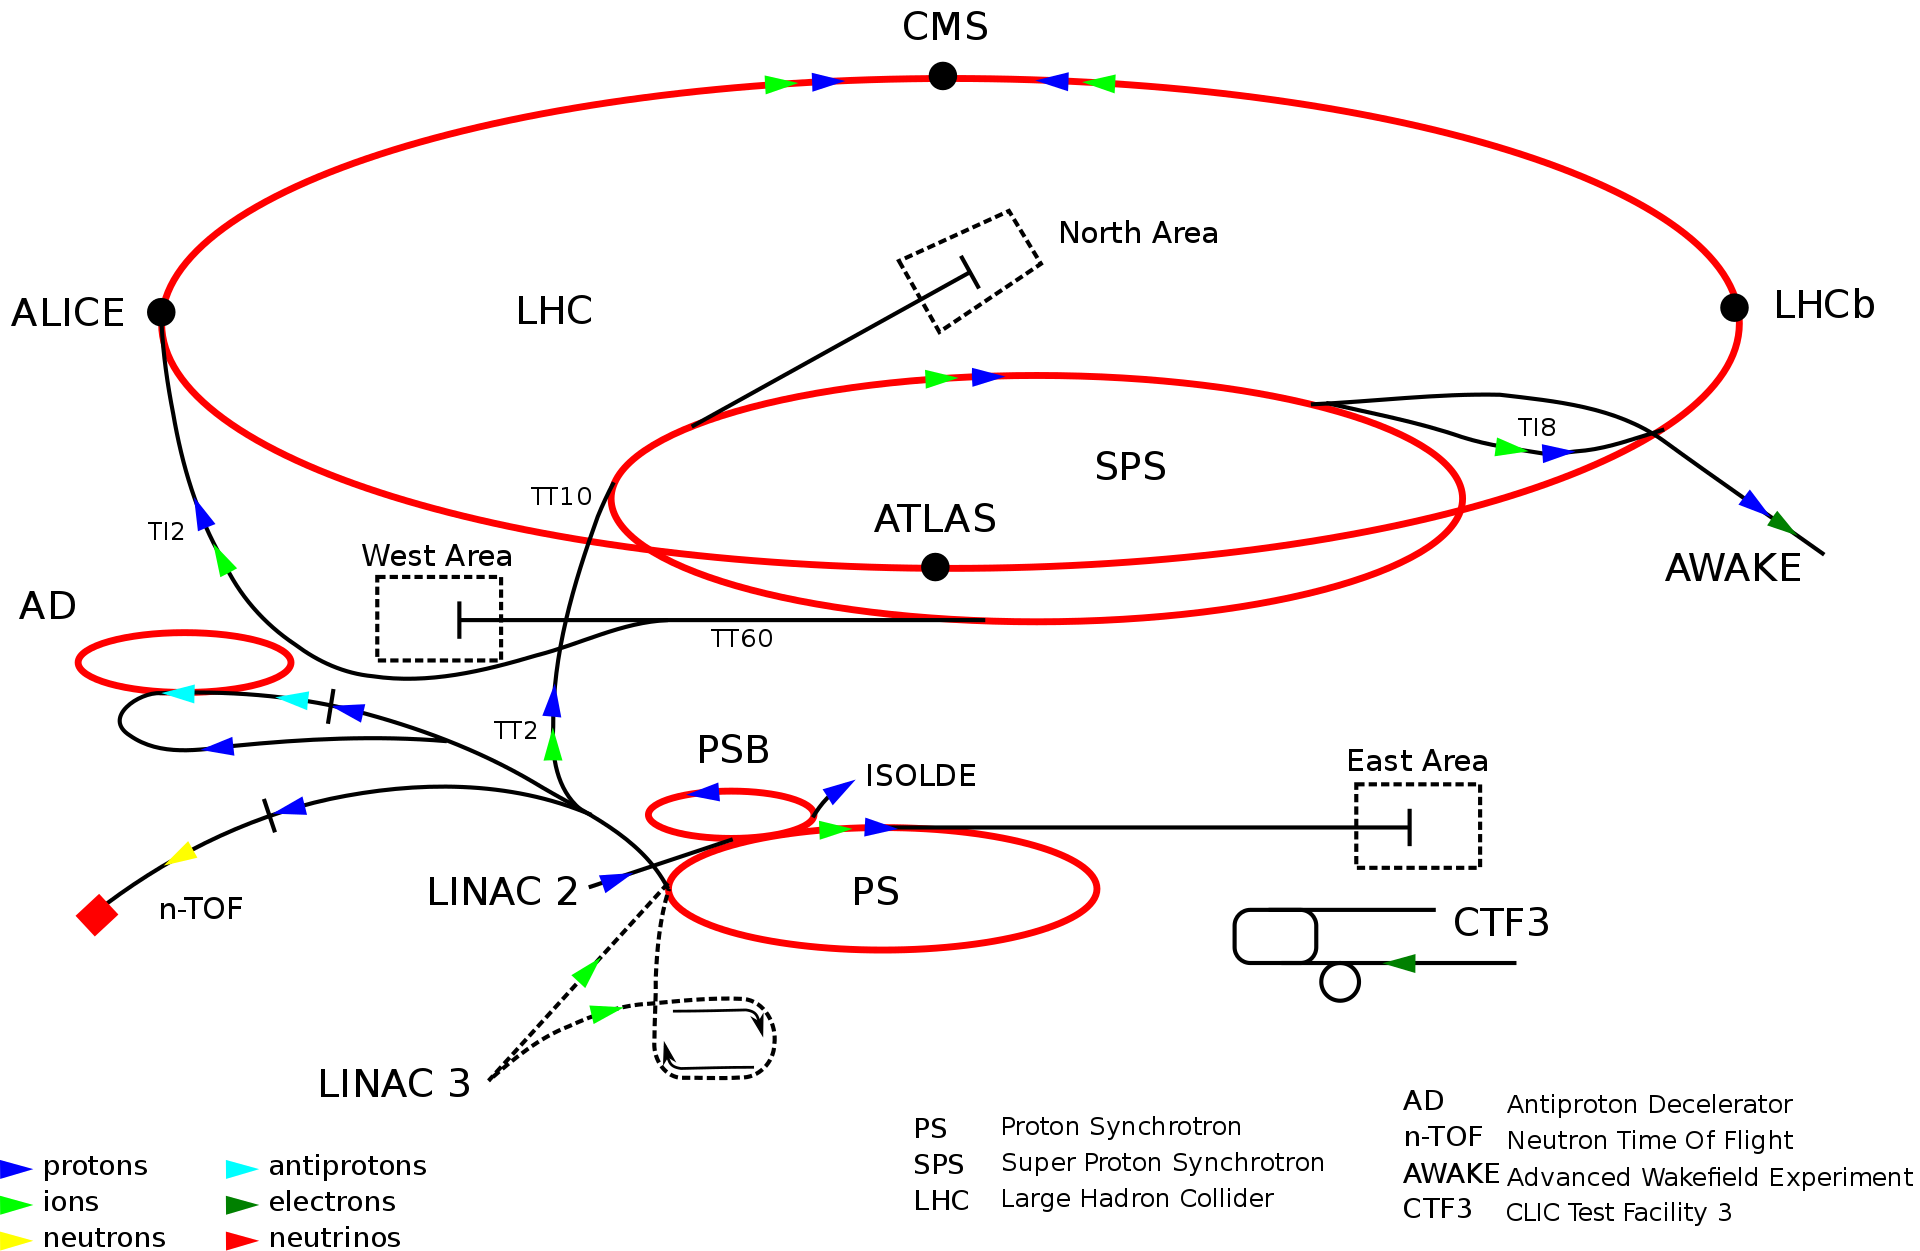
\includegraphics[width=0.8\textwidth]{CMS_experiment/LHC.png}
  \caption[Schematic representation of the LHC complex.]{Schematic representation of the LHC complex.}
  \label{fig:lhc}
\end{figure}

\hspace{10pt} The diversity of research areas covered by the LHC can best be seen in by looking at the coverage achieved by main experiments residing at four beam intersection points. Two general purpose experiments, ATLAS and CMS, take the center stage by being the main reason for the LHC's nickname. Adding the heavy ion research to the list, the ALICE experiment\footnote{With a help from the CMS experiment} takes the role of a primary experiment in within the field~\cite{ALICE_paper}. Finally, the LHCb experiment~\cite{LHCb_paper} proved crucial to the research ideas involving heavy flavour physics.

\hspace{10pt} The journey of a proton bunch begins with a canister of hydrogen gas, whose atoms are stripped from electrons by using an electric filed while the remaining protons are being passed on to the first step of acceleration - CERN's Linear Accelerator 2 (LINAC 2). Bringing the energy of particles to 50 MeV, it passes them on to the second step, the Proton Synchrotron Booster (PSB).  It further increases the energy of the particles reaching the values of 1.4 GeV before continuing towards the Proton Synchrotron (PS), where bunches reach the energies of 25 GeV. The final step in this process is the Super Proton Synchrotron (SPS) which brings the increase in energy to a total of 540 GeV. After this, particles are finally reaching the LHC, where their energy is further increased to a more desirable range of 7-14~TeV.


\hspace{10pt} The status of the LHC operation is best described when separated into three parts. During the writing of this thesis these could've been defined as the past, present and future of collider physics. Ranging from the period of 2009 to 2013, the past is manifested in the form of the Run 1 phase of operation. Colliding beams at 7 (and 8) TeV, the first cycle of operation brought in around $27~\text{fb}^{-1}$ of collected data, when looking from the CMS experiment's point of view. The beginning of this era was marked with a more than a year long delay, due to damage caused by an unexpected magnet quench. After the mandatory stop the journey was continued, first conservatively, by reaching energies of $1.18$~TeV per beam. This was enough to beat the previous record held by Tevatron collider (Fermilab)~\cite{tevatron_summary} and to put a first check on LHC's goal list. Increases in operational energy continued starting with $3.5~$TeV in 2010 and continuing in 2012, when the energy was set to $4$~TeV per beam marking the maximum reached during this stage. The most important achievement of this era (or better to say till this day) was the discovery of the Higgs boson in July of 2012. In order to be better prepared for the next stage, the LHC went into a shutdown period in 2013. 

\hspace{10pt} The first collision of $6.5~$TeV beams achieved on the 20th May of 2015 sounded the beginning of the current, Run 2, era of operation. Starting with the summer of 2016, the LHC reached its designed luminosity of $1.0\cdot10^{34}$~cm$^2$s$^{-1}$ (increasing it to twice the value before the shutdown). Brining in the total of $\sim130~$ fb$^{-1}$, Run 2 phase creates opportunities for precision measurements and probing of the BSM phase space (at the very least, excluding parts of it). Detector upgrades, some of which are going to be discussed in the following sections, brought a more efficient way of selecting relevant data by inserting complex, mode targeting selections early during triggering process. Currently, LHC experiments are working towards publishing a multitude of "legacy" results that are going to summarise and publicly release the conclusions made during this phase of operation.

\hspace{10pt} The future begins with the Run 3 phase of operation, which is expected to bring new ways of selecting data. Applying industry standard Machine Learning (ML) algorithms for research purposes, newly created triggers are expected to bring a significant increase in sensitivity for many of the BSM searches. Following this period, another upgrade stage is set to take place in order to prepare the machine for the next big step - the High Luminosity LHC. Figure~\ref{fig:lhc} showcases the LHC operation timeline with the projected integrated luminosity. 

\begin{figure}[htbp]
  \centering
    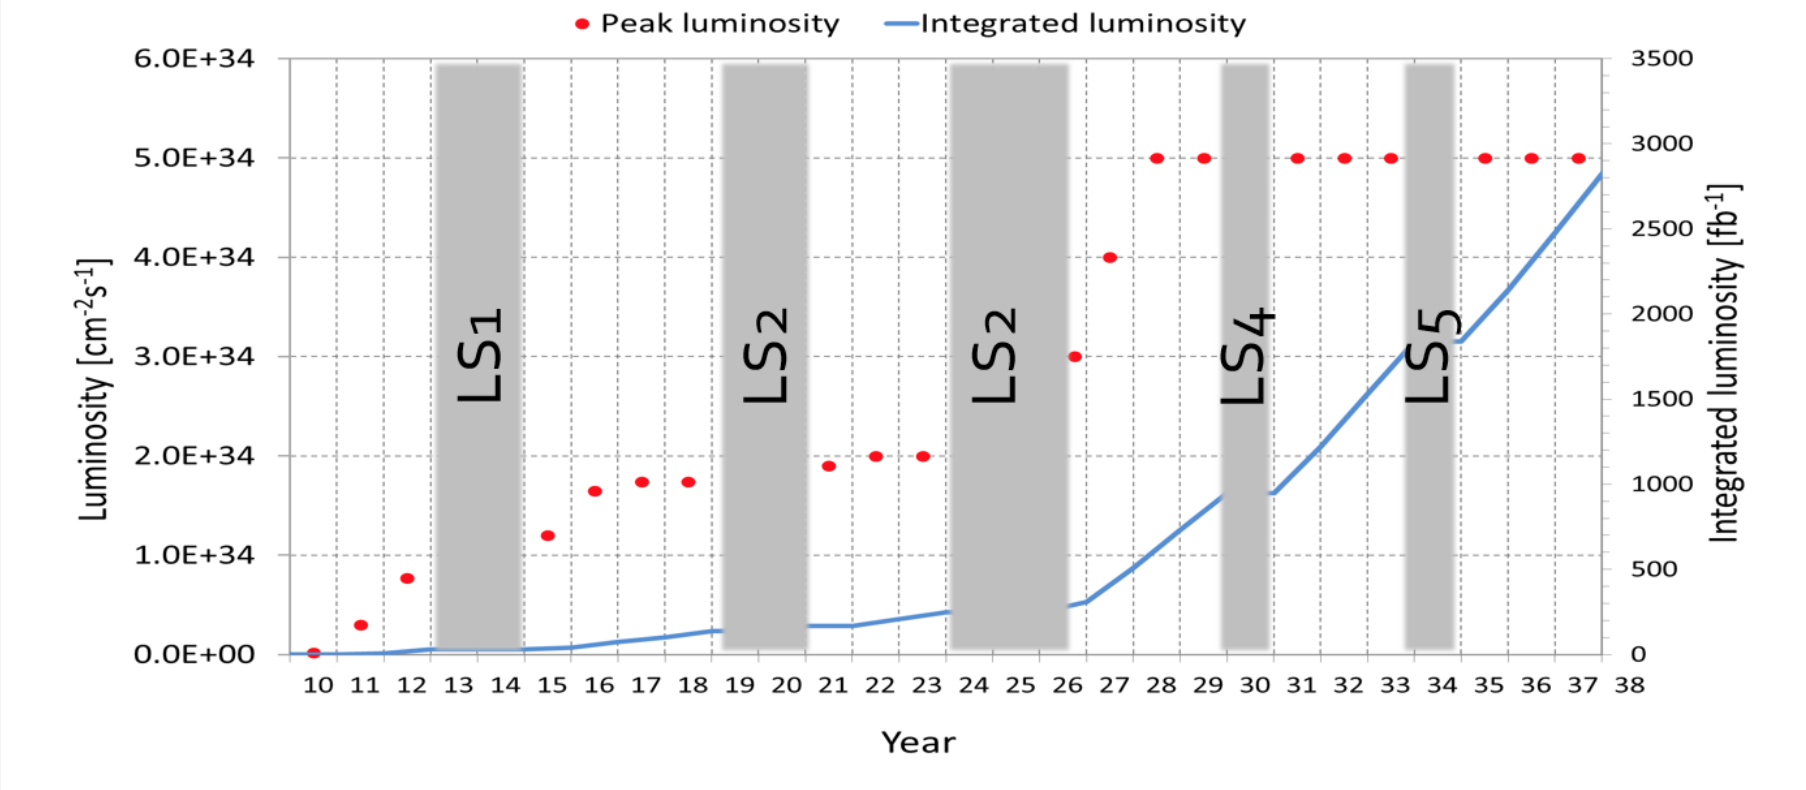
\includegraphics[width=0.95\textwidth]{CMS_experiment/LHC_integrated_lumi.png}
  \caption[Performance of LHC, extended to include the luminosity projections for up until the end of the HL-LHC phase.]{Performance of LHC, extended to include the luminosity projections for up until the end of the HL-LHC phase~\cite{ref:Schmidt_2016}}
  \label{fig:lhc}
\end{figure}


\hspace{10pt} Contents of the chapter following the completion of the LHC era are yet to be set in stone. A set of different proposals exist, with each of them having benefits and constrains in both monetary and physics sense of speaking. One highly advocated proposal is The Future Circular Collider (FCC) project~\cite{FCC_CDR}. It discusses a similar approach to one used with LEP/LHC years ago. During the early years of the project, an electron-positron collider would be built (FCC-ee) in order to probe the electroweak sector even further, while the technology is being prepared for the hadron collider (FCC-hh) that would bring the increase of the operational energy to the record level of 100~TeV. 



\subsection{The Compact Muon Solenoid}
\hspace{10pt} Taking the role of a leading general purpose detector\footnote{A completely unbiased observation by the author}, the CMS detector was designed to operate under proton-proton and ion collision beams with energies of 7 and 2.75~TeV respectively~\cite{cms:tdr}. It's design philosophy revolves around a few items, with the main, discovery of the Higgs boson, already  being marked as done early on during the initial Run 1 phase of LHC operation. As mentioned in the previous section, now the focus is to unravel what lies at the TeV energies, either through precision measurements and studies of known particles or by trying to search for new physics using theoretical models whose ideas can be quantified in a collider experiments. 



\section{Structure of the experiment}

\hspace{10pt}The CMS experiment itself is a cylindrical, layered detector comprised of several subsystems (as shown in Figure~\ref{fig:cms_slice}) working in harmony to help with particle detection and reconstruction. The subdetectors forming the CMS experiment are: the tracker, the electromagnetic calorimeter, the hadronic calorimeter, the superconducting solenoid, the muon chambers and the return yoke~\cite{cms:paper}. The general discussion of its operation can be split into two topics: the detection and data aquisition. Both of these will be covered in the following pages.
\subsection{Geometry}
\label{sec:geometry}
\hspace{10pt} The CMS experiment is positioned in a French village of Cessy, tucked in between beautiful sights of Jura mountains on one side and the city of Geneva from the other, allowing for a more descriptive approach when fixing the coordinate system~\cite{cms:tdr}. The main collision point is chosen to be the point of origin, from which the y axis follows the vertical line leaping towards the sky. The x axis is chosen as the one which points towards the center of the LHC ring, leaving the z axis to be the one that is tangent to the beam line, while also enjoying the view of the aforementioned mountains (as illustrated in Figure~\ref{fig:cms_coord_syst}).
\begin{figure}[htbp]
  \centering
    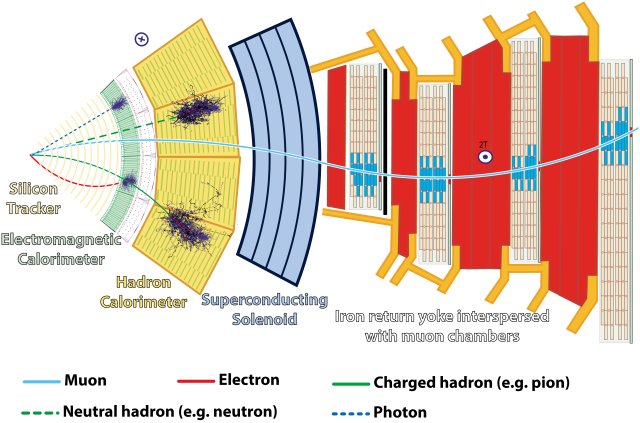
\includegraphics[width=0.85\textwidth]{CMS_experiment/CMSslice_whiteBackground.png}
  \caption[Transversal representation of different layers of the CMS experiment.]{Transversal representation of different layers of the CMS experiment~\cite{zCMS_slice}.}
  \label{fig:cms_slice}
\end{figure}
The definition of polar coordinates follows the standard procedure with the $\theta$ (polar) angle being defined from the z axis and the $\phi$ (azimuthal) angle being placed in the x-y plane starting from the x axis. In collider experiments it is usually easier do define alternative geometrical variables used to describe an object's position. This leads to the definition of peseudorapidity as: 
\begin{equation}
\eta = -ln\left [tan\left (\frac{\theta}{2}\right ) \right]
\end{equation}
Another variable commonly used to quantify the geometrical distancing of the particles is $\Delta R$. For two objects it is defined as:
\begin{equation}
\Delta R = \sqrt{\Delta\eta^2+\Delta\phi^2}
\end{equation}
Due to the structure of the CMS detector itself, it is important to define additional variables in the x-y, in further text the transversal (or the r-$\phi$), plane. Variables connected to it such as the transversal momentum and energy will be denoted as $p_T$ and $E_T$ respectively. The most important properties for this study are the missing transversal momentum and energy. They can be written as:
\begin{equation}
\begin{array}{l}
\vec{p}_{T, miss} = -\sum_i\vec{p}_{T,i},\\
E_{T, miss} = |\vec{p}_{T, miss} |,
\end{array}
\label{for:met}
\end{equation}
where the sum goes over all particles reconstructed by the detector. This imbalance in transversal momentum represents a valuable asset when quantifying the contribution of particles that are invisible to the detector. This will became more evident in the following chapters, where the $E_{T,miss}$ will be used extensively. 
Additional variables such as the transverse mass of a two body system, where particles masses can be neglected, can be written as:

\begin{equation}
    M_T = \sqrt{2E_{T,1}E_{T,2}(1-cos\Delta\phi)}.
\end{equation}

The following sections are going to further dissect the structure of the CMS experiment using the terminology introduced above. Two terms that will be a recurring item are the barrel and the endcap region representing a literal way of describing two general structural parts when discussing subdetector layers.
 
\begin{figure}[htbp]
  \centering
    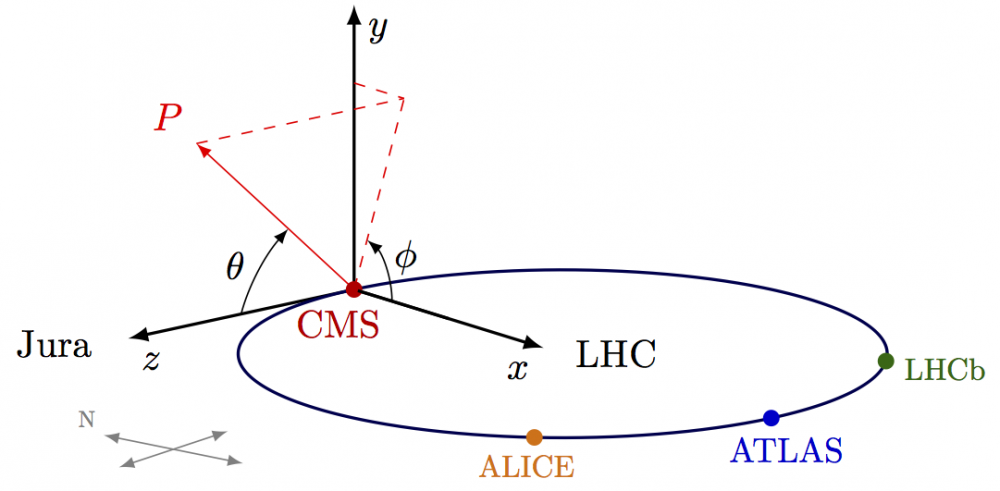
\includegraphics[width=0.8\textwidth]{CMS_experiment/cms_coordinate_system.png}
  \caption[Graphical representation of the coordinate system fixed to the CMS experiment.]{Graphical representation of the coordinate system fixed to the CMS experiment~\cite{coord_syst}}
  \label{fig:cms_coord_syst}
\end{figure}




\subsection{Tracker}
\hspace{10pt} The reconstruction of charged particle's track and the measurement of corresponding momenta is a crucial task for any collider experiment. The basis for tracking is formed around the interaction of charged particles with the atoms of the material they are travelling through. Said in a more precise way, the method revolves around exploring the trail of ionised atoms and free electrons left by particle moving in a magnetic field. If an electric filed is introduced in order to separate those electron-hole pairs, a current pulse will be created allowing for a "hit" signal to be detected.

\hspace{10pt} The, semiconductor based, tracking detector of the CMS experiment~\cite{cms:tdr}\cite{tracker_performance}\cite{Tracker:scheme} is positioned around the beam line, fully surrounding the interaction region as shown in Figure~\ref{fig:tracker}. It's design philosophy follows that it has to sustain the high collision rate given by the LHC, while providing the output in a form of particle tracks originating from the primary and secondary interaction vertices for the pseudorapidity range of $|\eta|<$2.5. The LHC input characteristics impose requirements that the tracker needs to have a high granularity structure, to provide longevity of the system and to have the ability to separate tracks originating from different bunch crossings (in other words, a fast enough response). All of this leads to the tracker being a fully silicon detector. The system itself is made out of two, operation independent, parts: the pixel detector (inner layer) and the the strip detector surrounding it bringing the total dimensions to 5.8~m in length with a 2.5~m in diameter (following the cylindrical design of the whole CMS experiment).
\hspace{10pt} 
\begin{figure}[htbp]
  \centering
    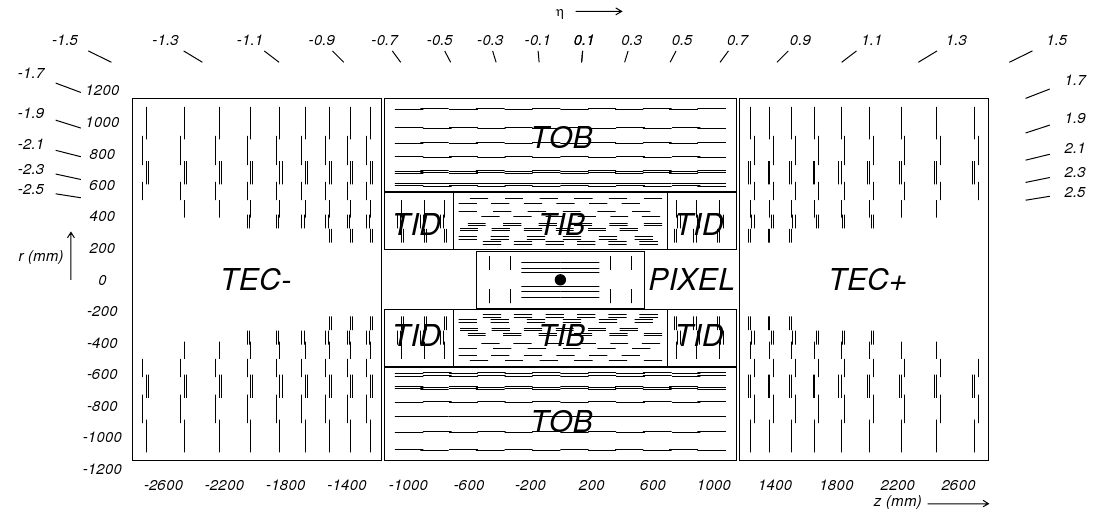
\includegraphics[width=\textwidth]{CMS_experiment/cmstracker.png}
  \caption[Structure of the CMS experiment's tracker system showcasing the subsystems in the barrel and endcap regions.]{Structure of the CMS experiment's tracker system showcasing the subsystems in the barrel and endcap regions~\cite{Tracker:scheme}.}
  \label{fig:tracker}
\end{figure}

\hspace{10pt} The pixel detector, covering the surface of 1.1~m$^{\text{2}}$, represents the first line of detection within the CMS experiment. Its barrel region (located within the $|\eta|<$0.9 range) is formed out of three cylindrical layers of detector modules with the radius being 4.4, 7.4 and 10.2~cm respectively. Forming the endcap region, additional two discs containing pixel modules are placed, completing the setup to a total of 66 milion pixels. It outputs three spacial points of detection associated to each charged particle in the event. The pixel subsystem represents an essential tool in reconstruction process of secondary vertices which play an important role in detecting heavy flavor and tau decay products. 

\hspace{10pt} The second part of the tracker, the strip detector, is made from a 10 layered barrel region and a set of 9 discs forming each endcap sides. The Inner barrel (TIB) and Discs (TID) form the first out of three main subsystems, delivering up to four detection points in the r-$\phi$ plane. The Tracker Outer Barrel (TOB) coveres the TIB and TID systems, allowing for additional points to be detected. Finally, shifting to the endcap region, there are the Tracker Endcaps (TEC+/-) providing up to nine $\phi$ detection points. Additional micro strip module is placed in all subsystems in order to enable the estimation of the missing component (r for the endcaps and z-axis position for the barrel).

\hspace{10pt} The importance of the tracking system is also seen in particle identification at the trigger decision level where the seed tracks are being constructed and passed as input data for the  trigger alogirthms to make an online decision.



\subsection{Electromagnetic Calorimeter}
\hspace{10pt} The next subsystem in particle's journey is the Electromagnetic Calorimeter (ECAL)~\cite{cms:paper}\cite{ECAL_performance}. It is comprised out of 75848 PbWO$_{\text{4}}$ (lead tungstate) crystals. The logic behind these types of detectors is based on the behaviour of high energy electrons and photons when passing through a material with a high atomic number Z. For the electrons, the main type of interaction with matter (in this energy range) is bremsstrahlung, while the photons interact through the electron-positron pair production. This, at the detector level, is cumulatively seen as an electromagnetic shower and is used to measure the energies of electrons and photons by amplifying the scintillation light produced in this process. Additionally to these e/$\gamma$ processes, there can be another contribution coming from $\pi^\text{0}$ decays to two photons originating from hardonic showers. The performance of the ECAL detector was crucial for the efforts towards the discovery of the Higgs boson. Its main driving force and ultimately its most important role was associated with searches within the $\text{H}\rightarrow \gamma\gamma$ decay mode (as well as the rest of modes containing $\text{e}/\gamma$ in its final state). 

\hspace{10pt} Scintilating crystals making the ECAL are chosen because of the compatibility of their properties with the expected performance of the LHC. The short radiation length (X$_\text{0}=\text{0.89}~\text{cm}$) ensures a small Moli\`ere radius (R$_\text{M}=\text{2.2~cm}$), allowing for compact dimensions of the detector. Being made out of a high density and optically clear crystal, ECAL can cope with the radiation impact as well as provide a compatibility with the bunch crossing time. The last statement translates into the fact that the majority of the scintillation light is being emitted in 25~ns. 

\hspace{10pt} The detector is made out of a barrel section which is hermetically sealed with the encap sections. The ECAL barrel (EB) section is responsible for energy deposits left within the $|\eta|<$1.47 range while the Endacap (EE) sections take over the responsibilities for the 1.68$<|\eta|<$3.0 range. The EB/EE crystals are $\approx$25/26 X$_\text{0}$ in length respectively. This choice of dimensions for the side facing the particle's trajectory is motivated by the size of the EM shower left in the crystal. Having such frontward crystal dimension simplifies the particle identification as the shape of the shower can easily be added as a selection criteria. A more visual overview is given in Figure~\ref{fig:ecal}, which showcases the structure of the ECAL where the aforementioned crystals are arranged in 36 supermodules. In order to have another helping hand, a preshower detector, which acts especially when it comes to $\pi^\text{0}/\gamma$ separation, is added to the setup. It is positioned in front of the EE rings covering the 1.64$<|\eta|<$2.5 region with its set of lead absorbers and silicon strip sensors.
\begin{figure}[htbp]
  \centering
    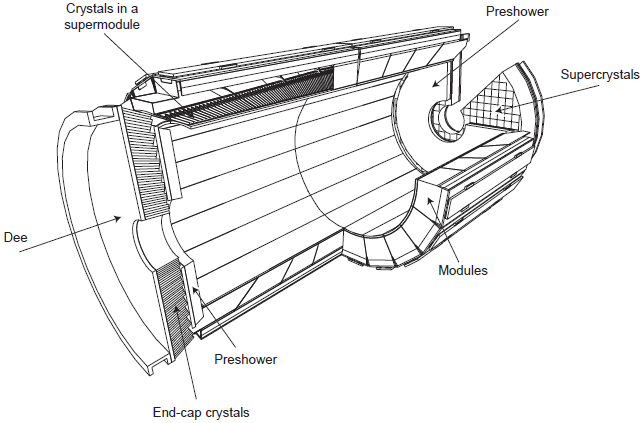
\includegraphics[width=0.8\textwidth]{CMS_experiment/CMS_ECAL.png}
  \caption[Schematic view of the CMS ECAL subdetector. The main susystems (EB, EE and the preshower detector) are presented as well their substructure]{Schematic view of the CMS ECAL subdetector. The main susystems (EB, EE and the preshower detector) are presented as well their substructure~\cite{cms:ecal}.}
  \label{fig:ecal}
\end{figure}

\hspace{10pt} With all the benefits that this choice of crystal structure brings, there are bound to be certain downsides. One additional property of lead tungstate cristals is that they have a very low light yield.  A set of signal amplifiers is needed in order to battle this disadvantage. For the EB region, a set of silicon avalanche photodiodes (APD) is used to boost the signal by a factor of $\sim$50 compared to the original. A similar scenario is deployed for the EE region, where vacuum phototriodes (VPT) with amplification ability of $\sim$10 times are used.

\hspace{10pt} The energy resolution of the ECAL detector can be parametrised as:
\begin{equation}
    \frac{\sigma^2}{E^2} =\bigg (\frac{A}{\sqrt{E}}\bigg )^2 +\bigg (\frac{B}{E} \bigg )^2 + C,
\end{equation}
where A, B and C represent the stochastic, noise and constant term respectively. The stochastic term is measured to be $2.8~$\% . The noise term, comprised form the cumulative effects of pileup, electronics and digitasion noise, has the value of $12~$\%. Finally, the constant term of $0.3~$\% is assigned to account for any leakage of energy or inter calibration errors. 

\hspace{10pt} The story of the ECAL will continue in Section~\ref{sec:data_acquisition}, where it will be showcased how these outputs are used at the first level of selection and beyond.
\subsection{Hadronic Calorimeter}
\hspace{10pt} Following a similar path derived for detecting the residuum of electromagnetic interactions of particles, a separate detector system has been added to measure the energies of hadronic showers - the Hadronic Calorimeter (HCAL)~\cite{cms:paper}\cite{hcal_performance}. When neutral and charged hadrons interact with the detector material through strong interaction, a hadronic shower will be formed with associated parameter $\lambda_{\text{i}}$, the nuclear interaction length. Representing a mean distance beween hadronic interactions within the shower, it takes much larger values than its electromagnetic equivalent, the radiation length. This would imply that the HCAL has to have large dimensions in order to be efficient, but on the other hand the compactness of the CMS detector fixes its position (and maximum dimensions) right in between the ECAL and the solenoid coil. This potential disadvantage is overcome with the structural design of the HCAL, which is made out of: barrel/endcap sections (HB/HE), a Hadron Forward (HF) subdetector and the outer barrel hadronic calorimeter (HO). Figure~\ref{fig:hcal} showcases the structure of the HCAL and all of its aforementioned parts.


\begin{figure}[htbp]
  \centering
    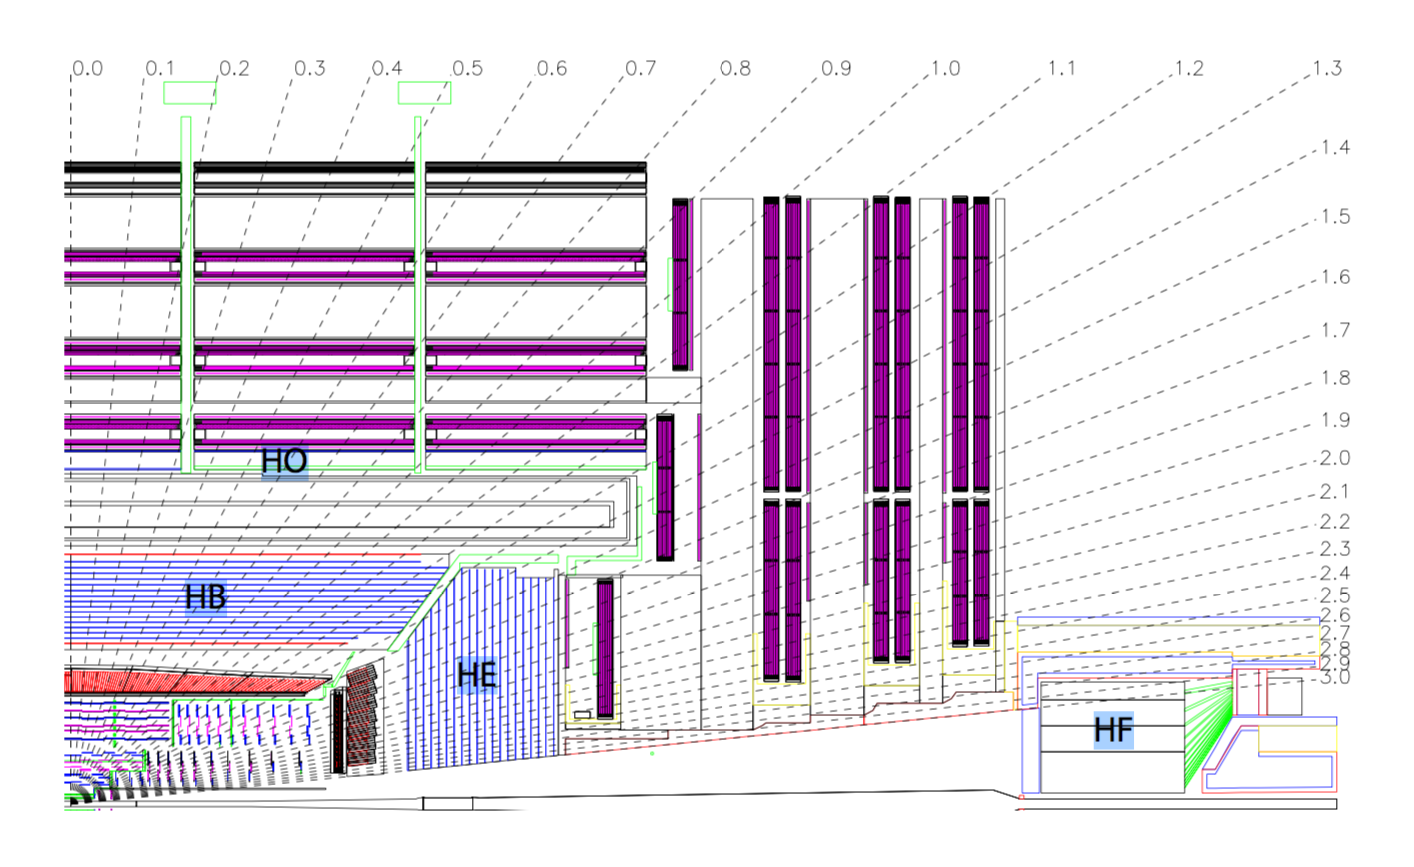
\includegraphics[width=0.95\textwidth]{CMS_experiment/HCAL_structure.png}
  \caption[Schematic ($\text{r}-\text{z}$) view of the CMS HCAL detector highlighting different subsystems: the hadronic barrel/endap (HB/HE), forward (HF) and outer (HO) detectors.]{Schematic ($\text{r}-\text{z}$) view of the CMS HCAL detector highlighting different subsystems: the hadronic barrel/endap (HB/HE), forward (HF) and outer (HO) detectors~\cite{cms:paper}}
  \label{fig:hcal}
\end{figure}

\hspace{10pt} The HCAL barrel is itself comprised out of two identical halves (HB$^{\text{+}}$/HB$^{\text{-}}$) covering the $|\eta|<$1.3 region. The subsystem is made out of layers of brass/steel (absorbing material) and scintillator tiles. A total of 32 identical wedges (each being segmented into four $\phi$ regions) made out of absorber plates form each of the barrel regions, with the scintillator tiles being positioned into 16 $\eta$ regions, bringing the total segmentation to ($\eta$, $\phi$) = (0.087, 0.087). The absorber itself is formed out of a front and back set of steel plates, in between which resides a group of 11 thick brass plates. The total thickness varies with $|\eta|$ from 5.8 until 10.6~$\lambda_{\text{i}}$ (for the edge values of $|\eta|=$0 and 1.3 respectively). On top of the HB thickness, there is a contribution coming from the previous detector, where the ECAL brings an additional 1.1~$\lambda_{\text{i}}$ to the total value. The scintialltor tiles are equipped with wavelength shifting fiber (WLS) readout, which is responsible for the transfer of emitted optical light. In order to battle the, previously mentioned, constrain in barrel dimensions, another subsystem is added after the solenoid structure (covering the $|\eta|<$1.26 region). The addition of the outer barrel hadronic calorimeter (HO) serves to effectively extend the size of the barrel section by moving the minimal thickness value up to 11$~\lambda_{\text{i}}$.

\hspace{10pt} Moving on to the endcap secion (HE), a set of two subsystems are put in place to be in charge of the 1.35$<|\eta|<$3.0 region following the same brass/scintillator structure used in the HB sections. Covering the diameter region starting from 0.8~m until 6.0~m, the endcaps have the same ($\eta$, $\phi$) segmentation as the HB sections for almost the entire $\eta$ range (the edge case being the $|\eta|\sim$3.0 region, where it doubles in value). A set of two forward calorimeters (HF) is placed behind the ends of the HE section. Each of them represents a Cherenkov detector comprised out of quartz fibers placed into iron and are used due to their radiation durable properties to extend the coverage up to $|\eta|<$5.2 (placing it really close to the beam line).


\subsection{Magnet}
\hspace{10pt} The central component of the CMS experiment (and one third of its name) is the 4~T superconductive solenoid~\cite{cms:paper} used to curve the trajectories of charged particles. It is 12.5~m long cylindrical structure with a diameter of 6~m. A high number of ampere-turns needed in order to generate such a strong field (41.7 MA-turns), introduced a new, four layer winding design which was a clear departure from solutions used with previous experiments (maximum of two layers). During run periods, the value it operates on is bellow its design value and stands at 3.8~T in order to ensure the durability of the system as a whole.

\hspace{10pt} Another important part of the magnet system is the return yoke. It is made out of 5 wheels in the barrel and 3 discs per endcap section interspersed alternately between layers of Muon chambers (described in the following section). Contibuting to the majority of the CMS experiments' weight, it stops almost all particles reaching it (minus the muons and neutrinos).
\subsection{Muon Chambers}
\label{subsec:cmsmuon}
\hspace{10pt} The final detector system discussed in this chapter are the muon chambers. Being a focal point for one of the main searches for the SM Higgs boson, the four muon final state represents the cleanest signature out of all other four lepton combinations due to the fact that muons are the least affected by energy loss in the previous sections (namely the tracker). This has influenced the way the CMS experiment was designed in a similar way how ECAL was connected to the diphoton final state. In order to approach the detection of muons, a setup is created through the use of three subsystems~\cite{cms:paper}\cite{muon_chambers_proceedings} based around gas chambers. 

\begin{figure}[htbp]
  \centering
    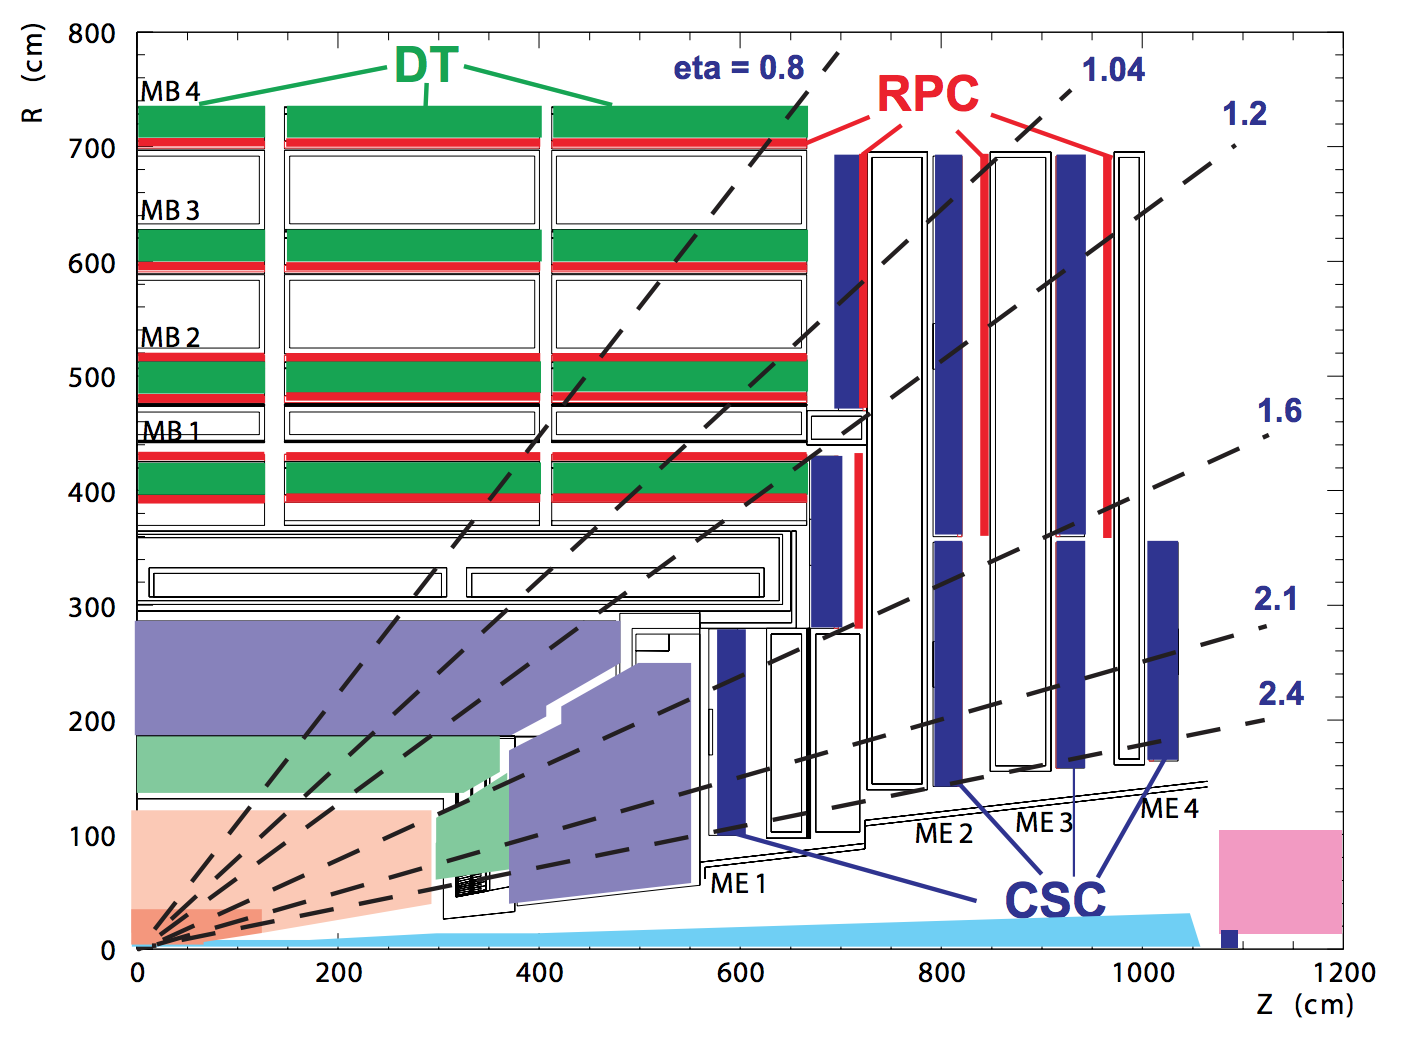
\includegraphics[width=0.95\textwidth]{CMS_experiment/Muon_chambers.png}
  \caption[Structural design of a ($\text{r}-\text{z}$) slice of the CMS Muon system highlighting different subsystems: the DT, CSC and RPC detectors.]{Structural design of a ($\text{r}-\text{z}$) view of the CMS Muon system highlighting different sections: the DT, CSC and RPC detectors~\cite{cms:tdr}}
  \label{fig:muon_chambers}
\end{figure}

\hspace{10pt} Starting from the barrel section, the $|\eta|<$~1.2 region is covered through the usage of Drift Tube (DT) chambers. From the stuctural point of view, each DT is made out of a streched wire placed in a gas volume. Comprised out of four stations inserted within the yoke, DT subsystem is responsible for measurement of muon's coordinates for this $\eta$ range. The first three inner stations (each containing 60 chambers) are responsible for mapping in both the r-$\phi$ plane as well as the z axis projection, while the last station (comprised out of 70 chambers) lacks the latter ability. For the encap region, a set of Cathode Strip chambers (CSC) is used instad of DTs. The change in the approach was introduced due to a much larger muon rate in this region, where radiation harder material and faster response given by the CSCs has proven to be a better option. 

\hspace{10pt} In order to battle the large amount of information, a dedicated trigger has been introduced to both DTs and CSCs. Based on the Resistive Plate chambers (RPC), this system is expected to provide fast triggering response over the majority of the $\eta$ range ($|\eta|<$1.6), helping out with muon track reconstruction scenarios starting from multiple hits per chamber (in case of DTs and CSCs). They employ the double gap chamber structure which in return provides good performance during full operation. The barrel section contains six layers of RPCs, while the endcap has areas covered with them for the first three sections, positioned in such way to complete the setup for an efficient (compact) muon detection system. 








\chapter{Data Acquisition}
\label{ch:daq}
%\label{sec:data_acquisition}
%\normallinespacing
\setlength\epigraphwidth{.8\textwidth}
\setlength\epigraphrule{0pt}
\epigraph{\itshape``It has long been an axiom of mine that the little things are infinitely the most important."}{--- \textup{Sir Arthur Conan Doyle, The Memoirs of Sherlock Holmes}}
%\mediumlinespacing
\section{Introduction}
\hspace{10pt} The sheer amount of data brought by the LHC brings a lot of opportunities for physicists to explore at the TeV scale. As it is usually the case, one advantage also brings a plethora of difficulties that need to be overcome, usually requiring a more practical approach. When looked at the maximum collision rate at the LHC (40~MHz), it can be seen that the total stress on the data acquisition system is around 40 million collision events per second, which is far beyond the reach of any currently available data storage systems. In order for the CMS experiment to be able to perform as efficiently as planned, a two stage structure was deployed with a task of discarding events deemed "unworthy" by its logic.

\hspace{10pt} Facing this problem head on, the CMS triggering setup consists of a, hardware based, first level of selection - the Level-1 Trigger (L1T) and a software High Level Trigger (HLT). The initial selection process done using the L1T scales down the total input rate to, a more approachable, 100~kHz. These decisions are based around a limited set of information coming from a set of subdetectors. The next stage in the triggering process, the HLT selection, is designed to further reduce the resulting output to $\sim$1~kHz of data, which is manageable by both the storage and offline reconstruction systems. Each of these triggering levels has a dedicated set of algorithms combined into a structure called the trigger menu. It is designed with the goal of allowing the passage of the appropriate rate of events expected from that system. The following sections are going to showcase the structure for each of these triggering levels, while focusing on examples relevant to the main study presented by this thesis.

 \section{Level-1 Trigger}
 \hspace{10pt} The starting point of this discussion is the, as the name suggest, first level of selection within the CMS experiment~\cite{cms:l1_paper}. It stands at the front line of data acquisition and is tasked with making a fast (in less than 4~$\mu$s) but sensible decision whether an event should be passed further down the chain. The core of the entire setup are the Field Programmable Gate Array (FPGA) boards. Their ability to perform faster parallel processing, re-programmability and the subsequent good price to performance/durability ratio, have lead to them being chosen instead of a CPU architecture. The many advantages that come with using the FPGAs in highly specialized tasks have lead to their wide spread usage, reaching even the video game industry\footnote{FPGAs are being used in modern recreations of 16-bit custom chips making the core of the fourth video game console generation such as the ones found in the Super Nintendo Entertainment System and Sega Mega Drive systems.}. The following pages are going to focus on the structure of the Level-1 trigger, relaying on a set of examples to efficiently explain its operation.
 
 \subsection{Overview}
 \label{l1:TTs}
 \hspace{10pt} The L1T forms a decision relying on the information coming form two centres: Calorimeters and Muon chambers. This can be seen in Figure~\ref{fig:l1_structure}, which shows the structure of the L1T system during the Run 2 phase of operation. Named after the corresponding information pool, the substructure of the L1T can be split into the Calorimeter and Muon trigger. The Calorimeter (Calo) trigger is comprised out of two layers and is responsible for the reconstruction, calibration and baseline identification of particles with ECAL/HCAL deposits: electrons/photons (e/$\gamma$), tau ($\tau$) and hadronic jets. The aforementioned jets represent a residuum of hadronic interaction located within a narrow geometrical cone. Due to the lack of tracker information at this stage, it is not possible to distinguish electrons from photons, which is why they are referred to as e/$\gamma$ objects. On the other hand, the Global Muon Trigger (GMT) is used to summarise the information gained from the three muon subsystems previously defined in Section~\ref{subsec:cmsmuon}. The starting point for both of these triggers is the same and comes from the information provided by the trigger primitives (TPs) which are formed from basic detector units.
\begin{figure}[htbp]
  \centering
    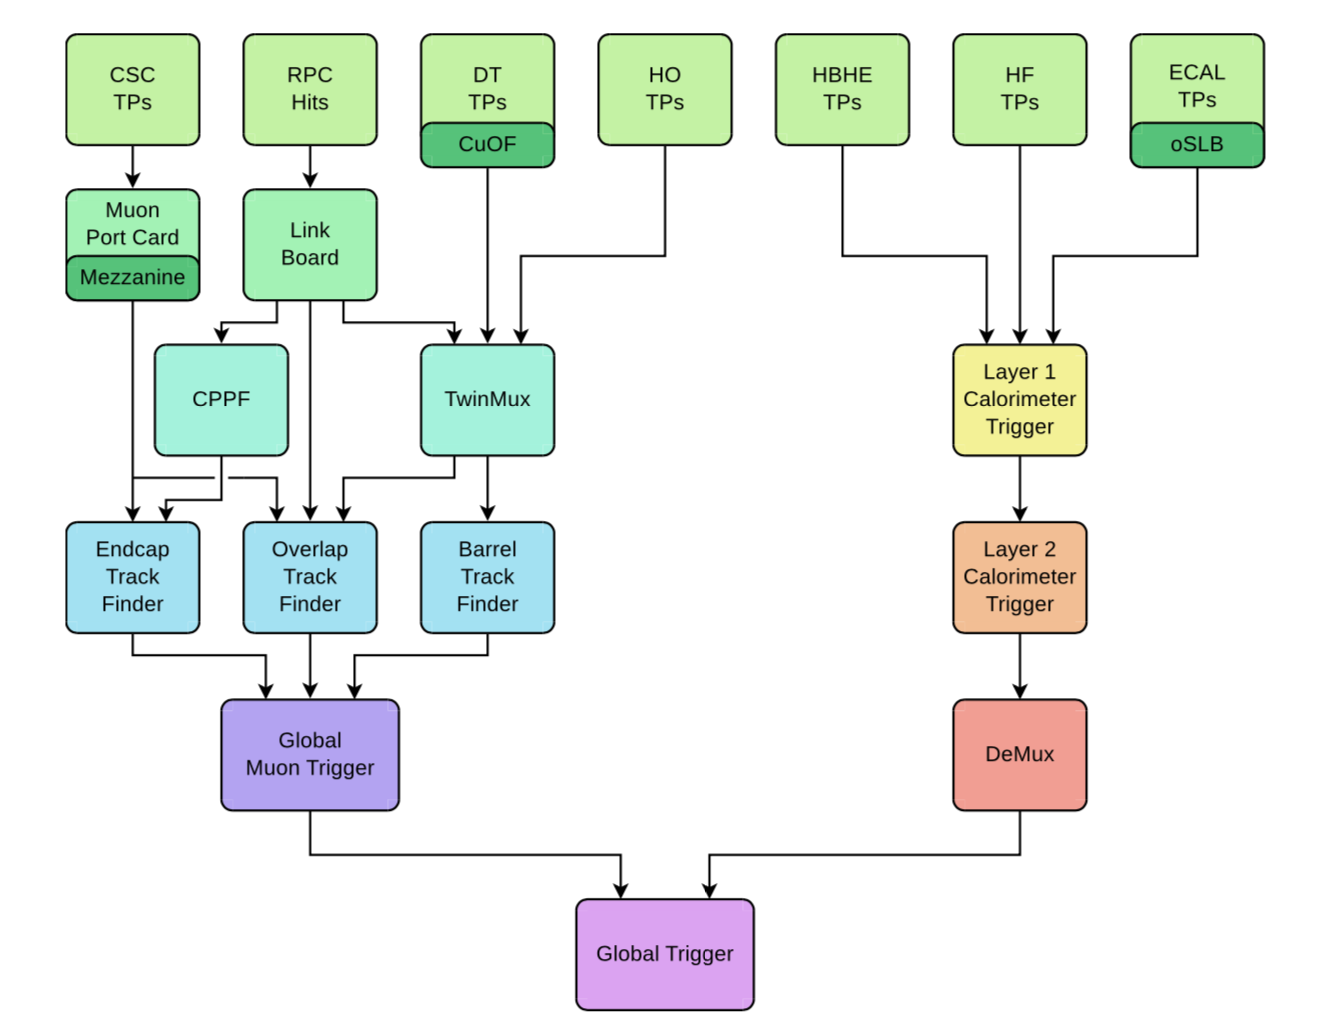
\includegraphics[width=0.95\textwidth]{CMS_experiment/L1_diagram.png}
  \caption{Structure of the CMS Level-1 system during its Run 2 operational phase.~\cite{cms:l1_paper}}
  \label{fig:l1_structure}
\end{figure}

\hspace{10pt} Figure~\ref{fig:l1_calo_trig} shows the structure of the Calo trigger. Detector inputs for this system are made out of Calo Trigger Towers (TTs). Each of these TT represents a 5x5 ECAL crystal structure combined with the HCAL tower positioned behind it [R] formed as such to take the advantage of the full detector granularity . The information (energy deposits) coming from TTs is passed to the Calo Layer-1. These deposits are then calibrated, corrected for additional detector effects (not accounted by the calorimeter electronics) and sorted preparing the input for the next step.

\hspace{10pt} The Calo Layer-2 is comprised out of a set of 9 FPGA cards (MP7), connected together in a round robin scheduling sequence. This Time-Multiplexed Trigger (TMT) design helps to extend the processing time given to each of the Calo Layer-2 cards. As an example, if each of the boards received information regarding one event per bunch crossing using this TMT design, this would increase the available processing time to be nine times larger than the standard bunch crossing time. At this stage, Calo L1 objects are being reconstructed from the available information using dedicated algorithms. The resulting data stream is being passed onto the De-multiplexing node (Demux), another MP7 board, with the task of retrieving the original event ordering before sending this information to the Global Trigger ($\mu$GT).
\begin{figure}[htbp]
  \centering
    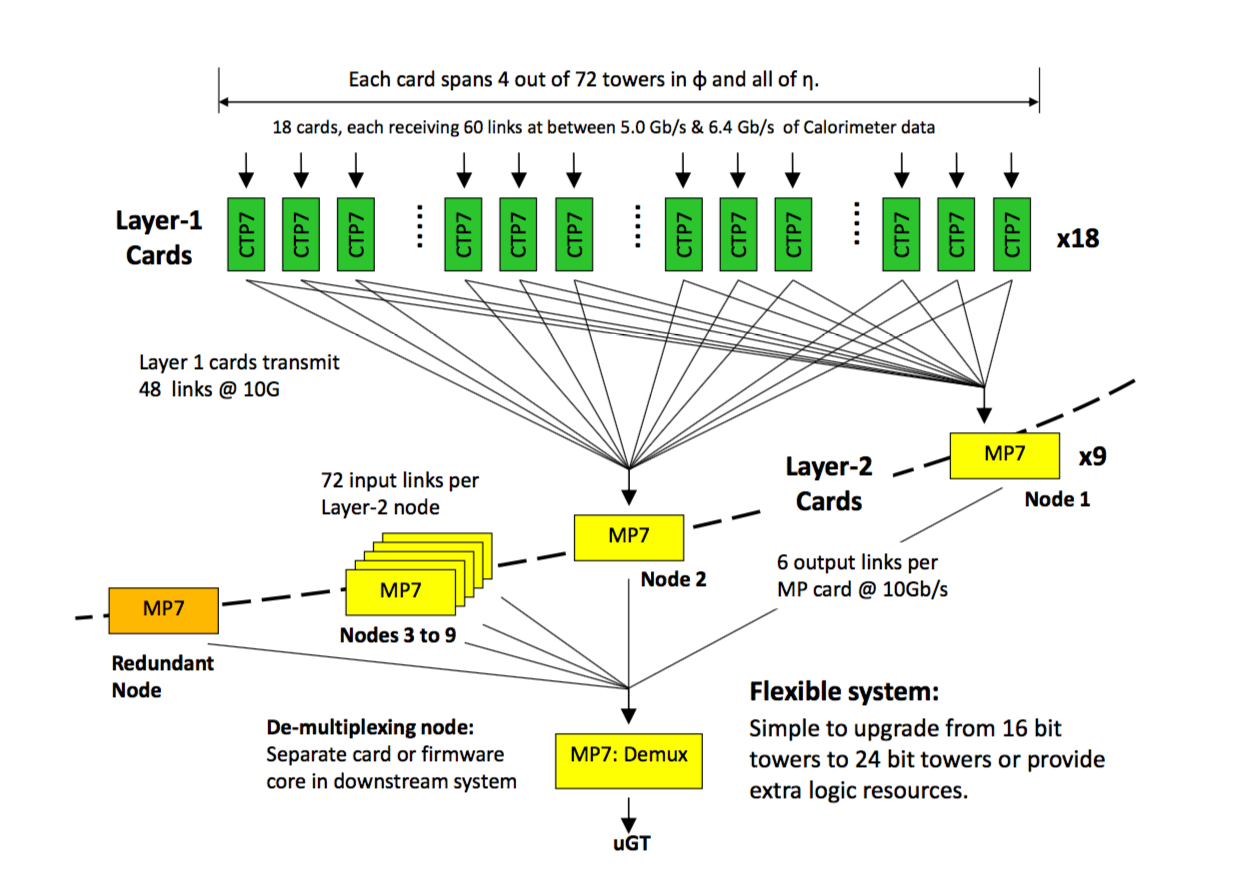
\includegraphics[width=\textwidth]{CMS_experiment/L1_calo_trig.png}
  \caption{Structure of the Calorimeter Trigger and its Time-Multiplexed Trigger architecture.~\cite{cms:l1_paper}}
  \label{fig:l1_calo_trig}
\end{figure}

\hspace{10pt} Due to their connection with the VBF production mode and the subsequent invisible final state of the Higgs boson, jets and energy sums will be used to illustrate L1T reconstruction algorithms~\cite{cms:l1_paper}\cite{Antoni}. Reconstruction of jets at L1T is performed through the usage of a dedicated algorithm. It focuses on a 9$\times$9 TT range surrounding the TT with the maximal deposit within the area, which satisfies the $E_T>$~4~GeV requirement. This TT range is chosen to mimic the geometrical ($\eta$, $\phi$) area used with offline jet reconstruction, which revolves around the $\Delta$R~$<$~0.4 cone. A simple comparison of energies with the TTs surrounding the central one are performed and the central TT is selected as a jet "seed" candidate if no other TT in the 9x9 area has energy larger/larger or equal than it. This additional equality comparison has been added in order to remove the possibility of the effect when TTs with same energies mutually veto each other. The chosen convention is shown in Figure~\ref{fig:l1_jet_chunky}. The total energy associated with the jet is then computed by summing the contribution from all TTs in the area, while the jet position is being fixed to the central seed TT. 

\hspace{10pt} Subtraction of the pile-up\footnote{Additional interactions whose resulting signatures are overlapping with the interaction of interest. It is coming from the fact that the LHC collides bunches of protons instead of a single pair.} contribution is done by using a set of four 3x9 TT structures, positioned next to the edges of the original 9x9 structure. This combined set of TTs bears a similarity with a "chunky doughnut", which is the initial idea behind the name of this jet pile-up removal algorithm. In order to avoid the scenario where a contribution coming from another jet structure would be removed, pile-up $E_T$ is computed using the sum of the three regions with the lowest energy which is then subtracted from the jet candidate energy.
 
\begin{figure}[htbp]
  \centering
    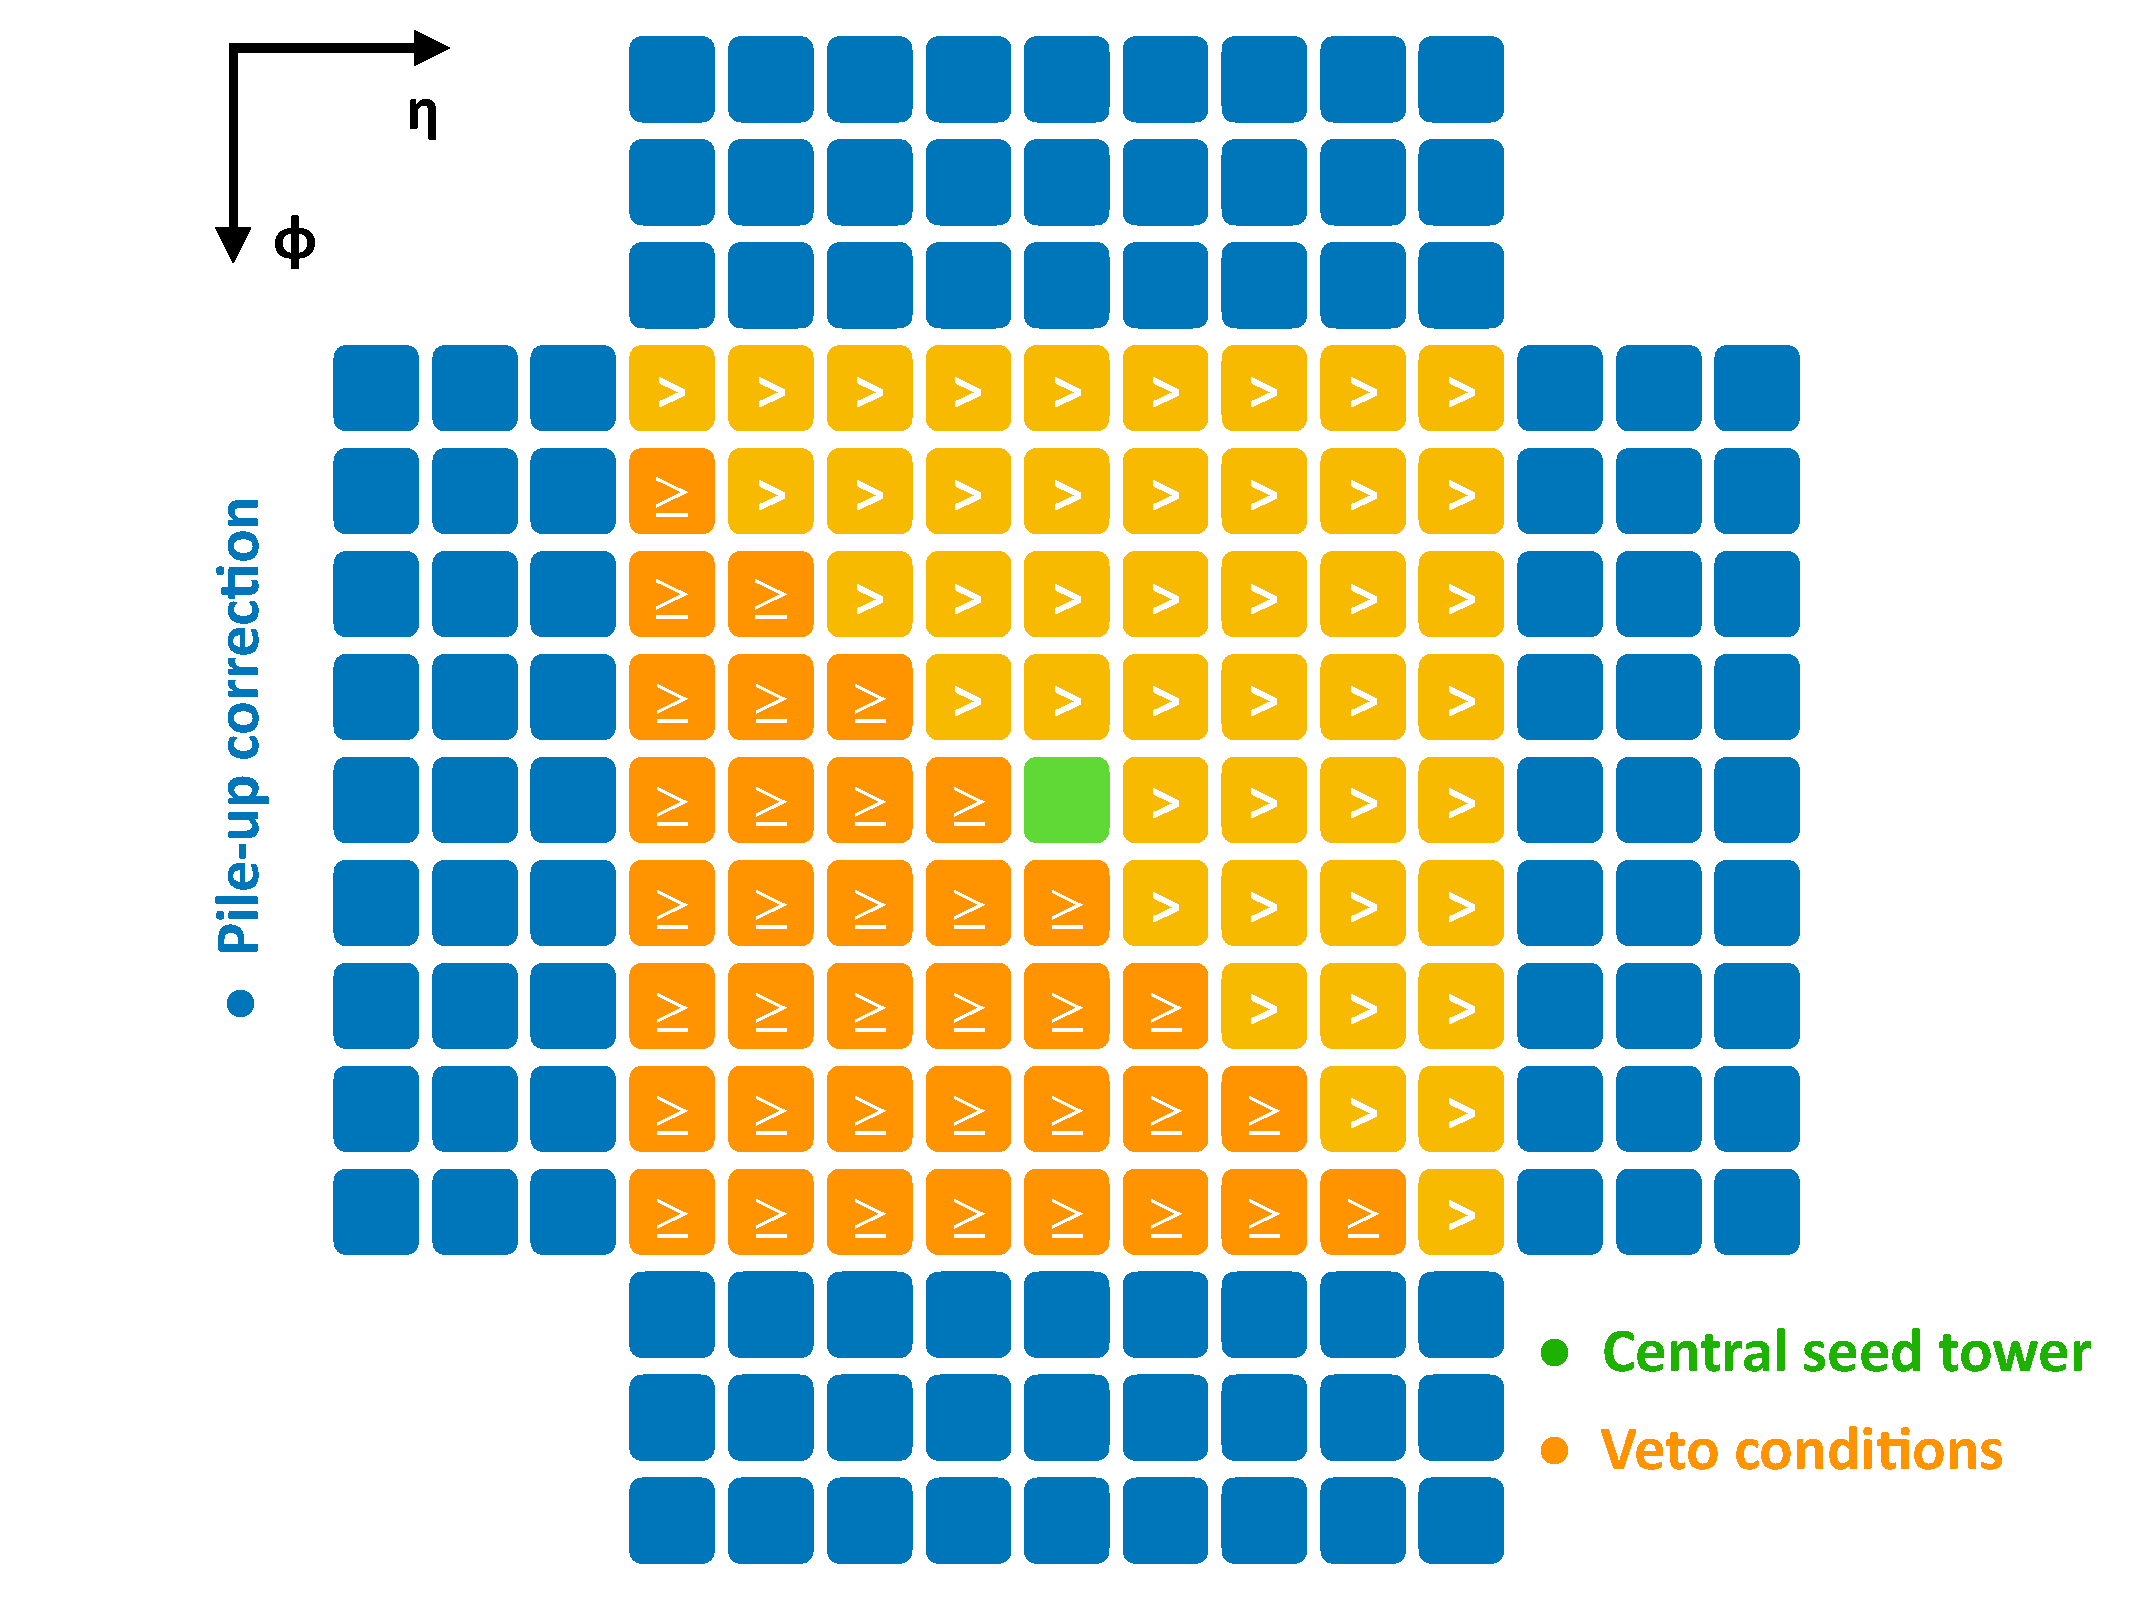
\includegraphics[width=0.9\textwidth]{CMS_experiment/jet_chunky.pdf}
  \caption{Graphical representation of 9x9 Calo TT formation used for L1T jet reconstruction, accompanied by 3x9 structures used for the pileup removal.}
  \label{fig:l1_jet_chunky}
\end{figure} 

Using the energies of the TTs it is possible to reconstruct the $\vec{p}_{T,miss}$ vector following the formula:
\begin{equation}
 \vec{p}_{T,miss} = -\sum_{i=1}^{n_{\eta}}\sum_{j=1}^{n_{\phi}}(E^{i}_{T}cos(\phi_j)\vec{e}_x + E^{i}_{T}sin(\phi_j)\vec{e}_y)
\end{equation}
 where (i, j) denote the sums over the ($\eta$, $\phi$) coordinates of TTs. Upon obtaining this property, the L1T $E_{T, miss}$ variable, extensively used when creating trigger paths listed in Table~{R} can be constructed as $E_{T, miss} = |\vec{p}_{T,miss}|$. Additionally, if the summation, when forming the previously defined property, goes over jet objects instead of all TTs, a new variable $\vec{H}_{T,miss}$ is created. 
 
\hspace{10pt} These physics objects reconstructed by the Calo Layer-2 are being passed on to the final step, the $\mu$GT, where they are combined with the information coming from the Muon trigger. At this stage, a decision is being made whether the event is going to be passed on to the HLT or discarded. In order to be able to make a decision, L1T uses a set of algorithms (seeds) which impose selection requirements on available physics objects. If the event passes all the requested qualities/thresholds and if the event is in accordance with the trigger rules, a Level-1 Accept (L1A) decision is being made and the event is passed on to the next step.

\subsection{Level-1 Trigger Menu}

\hspace{10pt} A set of aforementioned decision making algorithms, combined together through a logical "or", creates a structure called the L1T menu. The total rate of events selected by the menu is expected to be no larger than 100~kHz. In order to measure the collective rate given by the menu, an unbiased dataset (ZeroBias) is needed. The name ZeroBias is reflective of the fact that this data was collected using a selection that imposes only a single requirement: the event needs to contain a collision. 

\hspace{10pt}In order to control the total rate of events at the L1T, each seed within the menu has a "prescale" option inserted in the workflow. It provides the ability to limit the number of events passing the algorithm by scaling it down using a given integer value. This results in a scenario where, for a prescale value of 10, every tenth event which satisfies conditions imposed by the seed, is being allowed to advance to the next stage. 

\hspace{10pt} The implementation process for a new seed follows a standardised flow. Whether it being a simple or a complex algorithm, it's efficiency needs to be measured using Monte Carlo (MC) simulation samples that have been produced with appropriate object reconstruction. The increase in rate of the trigger menu associated with the addition of a new seed is called its pure rate. It has to be low enough for the trigger to be added to the menu, without removing/prescaling other seeds. The majority of the trigger menu rate is dedicated to seeds that have a wide spread usage in the later stages. Good examples of this are Single/Double lepton and $E_{T,miss}$ triggers, whose logic is presented in Table~\ref{tab:l1_triggers}. 

\begin{table}[htbp]
    \centering
    \begin{tabular}{lc}
     Algorithm & Requirements \\   \hline\hline
           & \\
      Single Muon   &  Tight Qualty \& $p_T>$22~GeV \\
                 & \\
      Double Muon  &  Tight Quality \& $p_T>$8~GeV  \\
                 & \\
      Energy sums ($E_{T}^{miss}$) & $E_{T}>$100~GeV \\
      & \\\hline\hline
    \end{tabular}
    \caption{A selected set of examples of most-used unprescaled trigger algorithms with their corresponding logics~\cite{cms:l1_paper}.}
    \label{tab:l1_triggers}
\end{table}

\hspace{10pt}For example, the lowest threshold, unprescaled single muon trigger is looking for a tight quality muon object that has $p_T>$~22~GeV. Muon objects that have been registered in at least three muon stations are marked down as tight quality objects. It is also possible to design triggers that would handle complex object manipulation. One of new seeds taking this advantage is created for the purposes of selecting VBF events. More details about this seed are going to be presented in Section~\ref{l1:vbf}. Finally, in order to safeguard the menu from any unforeseen rate problems, it is a common practise to have a few backup options for each seed. They are implemented with the same logic as the original, but with slightly higher thresholds on selection requirements. They provide viable replacements in situations when the menu rate is too high and the primary seed needs to be prescaled until the issue is fixed. 

\subsection{Level-1 Trigger pre-firing}
\label{sec:l1_prefire}
\hspace{10pt} Due to the heavy conditions under which the ECAL is exposed during LHC operation, a loss in transparency in its crystals began to affect its performance during 2016. With time this effect gradually increased, with the high $|\eta|$ regions being the most affected. This has introduced a timing offset in calibration of ECAL pulses, an effect that translated into resulting detector information which was turned into subsequent L1T Calo TPs. As a consequence of this, the Calo trigger information for the $|\eta|>$2.5 could be wrongly assigned to the previous (BX~$=$~-1) bunch crossing instead of the correct one (BX~$=$~0). This can lead to two major effects regarding the L1T decision.

\hspace{10pt} Firstly, it can lead to the effect called the L1T pre-fire in which the system wrongly distributes the information that the BX~$=$~-1 event passes its logic to the HLT. As this effect is not present with the offline reconstruction, a simplified version of which the HLT uses when reconstructing objects, pre-firing will cause the total loss of an interesting event. This comes from the fact that BX~$=$~-1 event will most likely be rejected at the HLT level due to the low probability that both BX~$=$~0 and -1  will contain interesting physics processes. On the other hand, accounting for the part of trigger rules which state that no more than one L1A decision can be made for three successive events (and no more than 2 L1As in a group of 25 successive events), the BX~$=$~0 event in this case is lost.

\hspace{10pt} Another scenario can happen due to a possibility of biased measurement of energy deposited in the Calo TPs. If the situation is reversed and the "early" signal does not invoke a positive L1A decision, there is still a problem as the, potentially interesting, BX~$=$~-1 information will be wrongly lost causing a bias in the energy measurement for the BX~$=$~0 event. 

\hspace{10pt} Unfortunately, a good example of a study affected by this issue is the VBF H$\rightarrow$inv analysis, due to its dependence of forward jets~\footnote{Jets within the forward region ($|\eta_j|>$~2.4)}. The effect of this has been studied at the analysis level for the data collected in 2016 [R] and the results state that a correction ranging from 1-20~\% needed to be applied (depending on the fit variable range), which resulted in a total loss of $\sim$17~\% of the expected sensitivity towards the BR(H$\rightarrow$inv). More details about the corrections of this issue for the data collection era of 2017 are given in Section~\ref{sec:objects}.


\section{Online Data Quality Monitoring}
\hspace{10pt} In order to have constant surveillance of the operation of the CMS experiment, three daily shift crews are placed at the control cavern at of the detector (positioned at the LHC Point 5). The constant monitoring of L1T menu rates is needed to quickly account for any unexpected increases, by prescaling problematic seeds. On the other hand, in order for the shifter to be able to monitor the performance of the L1T, as set of  informational plots and alarms is displayed as a part of the data quality monitoring (DQM) package~\cite{Antoni}. Taking into account that the knowledge possessed by the shifter is usually not on the level of a L1T expert, a separation of plots is being made into two groups: shifter and expert, where the latter contains much more details (i.e. the full Calo granularity information) needed for debugging.

\hspace{10pt} Taking the Calo trigger as the example, in order to have a separate control system, an emulator software was written in C++ and optimised for a CPU architecture with the same logic as the one used on the trigger boards (both the MP and Demux nodes). This emulator was made a part of a standardised CMS Software Framework (CMSSW), which helps with the general ease of use and software compatibility. In order to monitor the performance of the Calo trigger during run periods an online DQM package was deployed containing several main checks needed for validation.

\hspace{10pt} There are several types of plots needed to efficiently control the operation of the Calo Layer-2 during data taking periods. One of the first checks would be to plot the distributions of main properties of physics objects in order to quickly spot any anomalies in the reconstruction. On the other hand, the "data to emulator" plots sorted either by the overall agreement or disagreement between the firmware and the emulator represent a systematic way of ensuring early problem detection.  A select set of example plots summarising this setup are given in Figure~\ref{fig:dqm_plots} 
\begin{figure}[htbp]
  \centering
      \subfigure[A]{
    \includegraphics[width=0.45\textwidth]{example-image-a}
    }
    \subfigure[A]{
    \includegraphics[width=0.45\textwidth]{example-image-a}
    }\\
    \subfigure[B]{
    \includegraphics[width=0.45\textwidth]{example-image-a}
    }
    \subfigure[B]{
    \includegraphics[width=0.45\textwidth]{example-image-a}
    }\\
    \subfigure[C]{
    \includegraphics[width=0.45\textwidth]{example-image-a}
    }
    \subfigure[C]{
    \includegraphics[width=0.45\textwidth]{example-image-a}
    }
  \caption{DQM Example plots - TBA as soon as I get the online playback running.}
  \label{fig:dqm_plots}
\end{figure}


\section{High Level Trigger}

\hspace{10pt} The second step of trigger selection operates under more manageable input conditions, allowing for a few hundred millisecond decision making time window. This has enabled the more traditional, high level software, design of the High Level Trigger (HLT)~\cite{HLT_performance}. It is based on a set of algorithms (paths) written in C++, that are deployed on a server farm comprised out of Intel Xeon CPU based machines.

\hspace{10pt} This additional timing allows for more complex object reconstruction, which is why the HLT uses a simplified version of the Particle Flow (PF) algorithm in order to take the advantage of the full detector information. More details about the PF algorithm itself will be given in Section~\ref{sec:objects}. The main feature of the HLT is its modular design. A collection of C++ modules allows experts to build more detailed selection requirements. A module can take a role of a producer of $E_{T,miss}$ variable from given PF candidates, it can impose a selection requirement on a given variable and many more. Each module is required to be made as a template structure and included in the CMSSW framework. An HLT path is created through combination of different modules through a chain of intermediate decisions. This leads to another reduction in rate, resulting in the output of $\sim$1~kHz that gets passed on to the final step, the full reconstruction and storage of events.

\hspace{10pt} A more user friendly approach to managing available HLT modules is enabled through the usage of the "confDB" software~\cite{confdb}. Written in java language, it's main purpose is to help with the creation of new HLT paths. It provides a GUI environment which can be used to easily import modules into newly created structures as well to set their default properties. As briefly mentioned before, an HLT path represents a flow of decision making modules starting from the information gained from desired input L1 seed. The process of making and deploying an HLT path will be the focus of the next section, using the implementation of VBF production mode targeting triggers as an example.

\hspace{10pt} In order to deploy an HLT path, approval procedure, similar to the one used with L1 seeds, needs to be followed. The first item on the checklist is to prove the physics motivation for the trigger. This is usually done through a study of an efficiency gain compared to previous algorithms. Following that, a more technical part of the process needs to be done. Measurements of pure rate and timing need to be performed and checked before adding the path to the official menu. The addition of timing is important due the fact that this is a fully software trigger using a simplified version of the PF algorithm, which is its biggest offender. This control of timing will be discussed in the following section.

\newpage
\section{Triggering of VBF events}
\label{sec:vbf_trgger}
\hspace{10pt}Historically, the search for the invisible decays of the Higgs boson has been built around $E_{T,miss}$ and $H_{T,miss}$ based triggers. The similar statement holds true for many of searches for the BSM physics at the CMS experiment, which is why these triggers gained status of general purpose algorithms. This was enabled by checking two main goals when it comes to defining a multi purpose trigger. Firstly, they were interesting to the analysers as they only imposed selection requirements on a very few variables during the triggering process. This, in return, allowed for any additional object manipulation to be done in the offline analysis\footnote{After the full object (offline) reconstruction and storing of events.}, without having a constrain coming from events not being stored. The second point was extremely important when looked from the organisational perspective. As these triggers were used by more analysis groups studying different signals containing particles invisible to the detector, it became easier to justify the amount of rate allocated to these paths, which resulted in a set of generously tailored selection requirements.

\hspace{10pt} The previous statement in no way sounds the end of the story, as even with a more relaxed set of requirements, the very idea of the search is dependant on having the lowest possible threshold on the "invisible" contribution. There were several attempts at creating triggers based around a set of crude HLT level decisions following the VBF topology. The main idea behind these triggers was that, by adding kinematic requirements on the jets, the rate would be reduced enough to allow for an even lower selection threshold on $E_{T,miss}$. This provided mixed results and a more viable solution was continued to be sought after.


\subsection{Overview of the VBF Level-1 trigger}
\label{l1:vbf}
\hspace{10pt} The situation changed for the better, when it comes to analysis specific HLT algorithms, in recent years. Following the recent upgrade of the L1T~\cite{cms:l1_paper}, analysts were given the opportunity to impose a set of requirements including complex object manipulation even at this first stage of decision making. This new feature has led to the creation of dedicated L1T seeds specifically targeting the VBF production mode of the Higgs boson (in further text referred to as VBF L1 seed). This has opened a door for a new set of HLT paths, which will tailor the selection towards the invisible final state. Serving as an example of the HLT trigger implementation procedure, the following section is going to describe the idea behind a set of HLT paths deployed during the mid stage of the Run 2 phase.

\subsection{Implementation of VBF High Level Triggers}
\label{sec:vbf_implementation}
\hspace{10pt} The base logic of the aforementioned L1 VBF seed, was created by transforming the physical properties of the VBF production mode into a set of decisions that can be interpreted at the first stage of the CMS triggering system. This mode targeting algorithm was built from the benefits given by the recent upgrade of the L1T, allowing for complex object manipulation. One of these variables interesting for the VBF production mode was the invariant mass of a dijet pair (dijet mass). It is defined as:
\begin{equation}
    m_{j_1,j_2} = \sqrt{2\cdot E_T^{j_1}\cdot E_T^{j_2}\cdot [cosh(\Delta\eta_{j_1,j_2})-cos(\Delta\phi_{j_1,j_2})]},
\end{equation}
where $E_T^{j_{1/2}}$ denote transversal energies of L1 jets and $\Delta\eta_{j_1,j_2}$/$\Delta\phi_{j_1,j_2}$ measure their geometrical separation in the ($\eta$/$\phi$) plane. It provided a valuable tool in reducing the rate of the trigger, while ensuring a minimal loss of desired signal sensitivity. Translated into the actual algorithm logic, this approach states that the event passes the L1T requirements if it contains both of these two scenarios~\cite{cms:l1_paper}:
\begin{itemize}
    \item The event contains at least two L1 jets that pass: $E_T > 110,~35~(115,~40)$~GeV
    \item There exists a dijet pair, whose invariant mass $m_{jj}  > 620$~GeV, where the jets forming it also pass $p_T > 35~(40)$~GeV requirement
\end{itemize}
The first era of using this seed (2017) brought its fair share of problems which increased the rate of L1 seeds targeting forward jets. This manifested itself in the fact that the L1 jet thresholds had to be much higher than expected in order to contain the rate within reasonable boundaries. This forced the experiment into activating additional backup seeds, listed in Table [R] during this period. As the time passed, CMS trigger experts managed to implement a correction for this effect while also relaxing a part of its bandwidth, which allowed for the lower threshold seeds to be reinstated into the triggering menu during 2018. More details about the process of implementation and the performance of this seed can be found in~\cite{cms:l1_paper}\cite{Chiara}.

\hspace{10pt} As a mean to actually explore this newly available phase space at the analysis level, a set of second level decisions were combined to create new HLT paths. The main idea behind them was to take the events passing the VBF L1 seed and imposing a groups of kinematic requirements on PF reconstructed jets (mimicking what was done at the L1T stage), while matching the PF to the L1 jets. Second step was to further tailor this selection to the "invisible" final state by adding $E_{T}^{miss}$ requirements. The final goal was to have a reduction of rate coming from jet conditions being large enough to be able to justify a more relaxed set of $E_{T}^{miss}$ thresholds. The following points summarise the HLT requirements:
\begin{itemize}
    \item $E^{Calo, NC}_{T,miss}>66$~GeV requirement on $E_{T,miss}$ reconstructed from the calorimeter information only, which has been cleaned from the HCAL noise;
    \item $E^{PF}_{T,miss}>110$~GeV requirement on $E_{T,miss}$ reconstructed from all PF object candidates;
    \item Usage of a custom made module for the purpose of matching the L1 jet collection with the PF jet collection as well as for the application of additional kinematic requirements on the jets;
    \item Further separation into two and three jet categories based on the output of the previous step.
\end{itemize}

Starting with the jet part of the algorithm. First, events are pre-filtered based on a flag specifying whether the event passes a logical "or" of all L1 VBF seed variants. For the passing events, the L1 jet collection is being matched to the PF jets that have $p_T>35$~GeV, using the geometrical cone of $\Delta R<0.5$ as its matching criteria. Upon obtaining this new collection of PF jets, they are required to fall under one of two options (otherwise the event is failed):
\begin{itemize}
    \item Option A: All possible dijet pair variations are created in order to find the combination which yields the largest dijet mass, with that value having to be greater than $650$~GeV. After selecting the pair, it is required that the higher $p_T$ jet passes  the $p_{T,j}>110~$GeV threshold.
    
    \item Option B: Jets forming the largest dijet mass in the event must pass the $p_{T,j}>35~$GeV requirement, while the dijet mass must be larger than 650~GeV. Neither jet from the pair is allowed to have $p_T>110$~GeV. Upon obtaining the dijet pair, the leading jet in the collection is being looked at in terms of $p_T$. If it passes $p_T>110$~GeV requirement, all three jets are selected and the event advances to the next stage.
\end{itemize}
After collecting the two possible scenarios, the final module of the path selects either the two jet (option A) or the three jet (option B) case, thus forming the two paths shown in Table~\ref{tab:hlt_rates}. The structure and decision flow of these paths containing all of the modules is displayed in Figure~\ref{fig:VBF_HLT}.
\begin{figure}[!htbp]
  \centering
    \includegraphics[width=\textwidth]{CMS_experiment/VBF_HLT_structure.pdf}
  \caption{Modular structure of the VBF HLT paths. The common flow starting with the input decisions inherited form the VBF L1T seeds is shown for both the dijet and triple jet HLT paths.}
  \label{fig:VBF_HLT}
\end{figure}

\hspace{10pt} Moving on to the $E_{T,miss}$ part of the requirements. As mentioned above, certain requirements have been introduced in order to control issues of rate and timing. A certain threshold on the $E^{PF}_{T,miss}$ had to be introduced in order keep the rate within a reasonable range. Figure~\ref{fig:PFMETvsRate} shows the estimate of the total rate of the dijet path and highlights the final choice of $E^{PF}_{T,miss}>$~110~GeV as the minimal sustainable value.
\begin{figure}[!htbp]
  \centering
    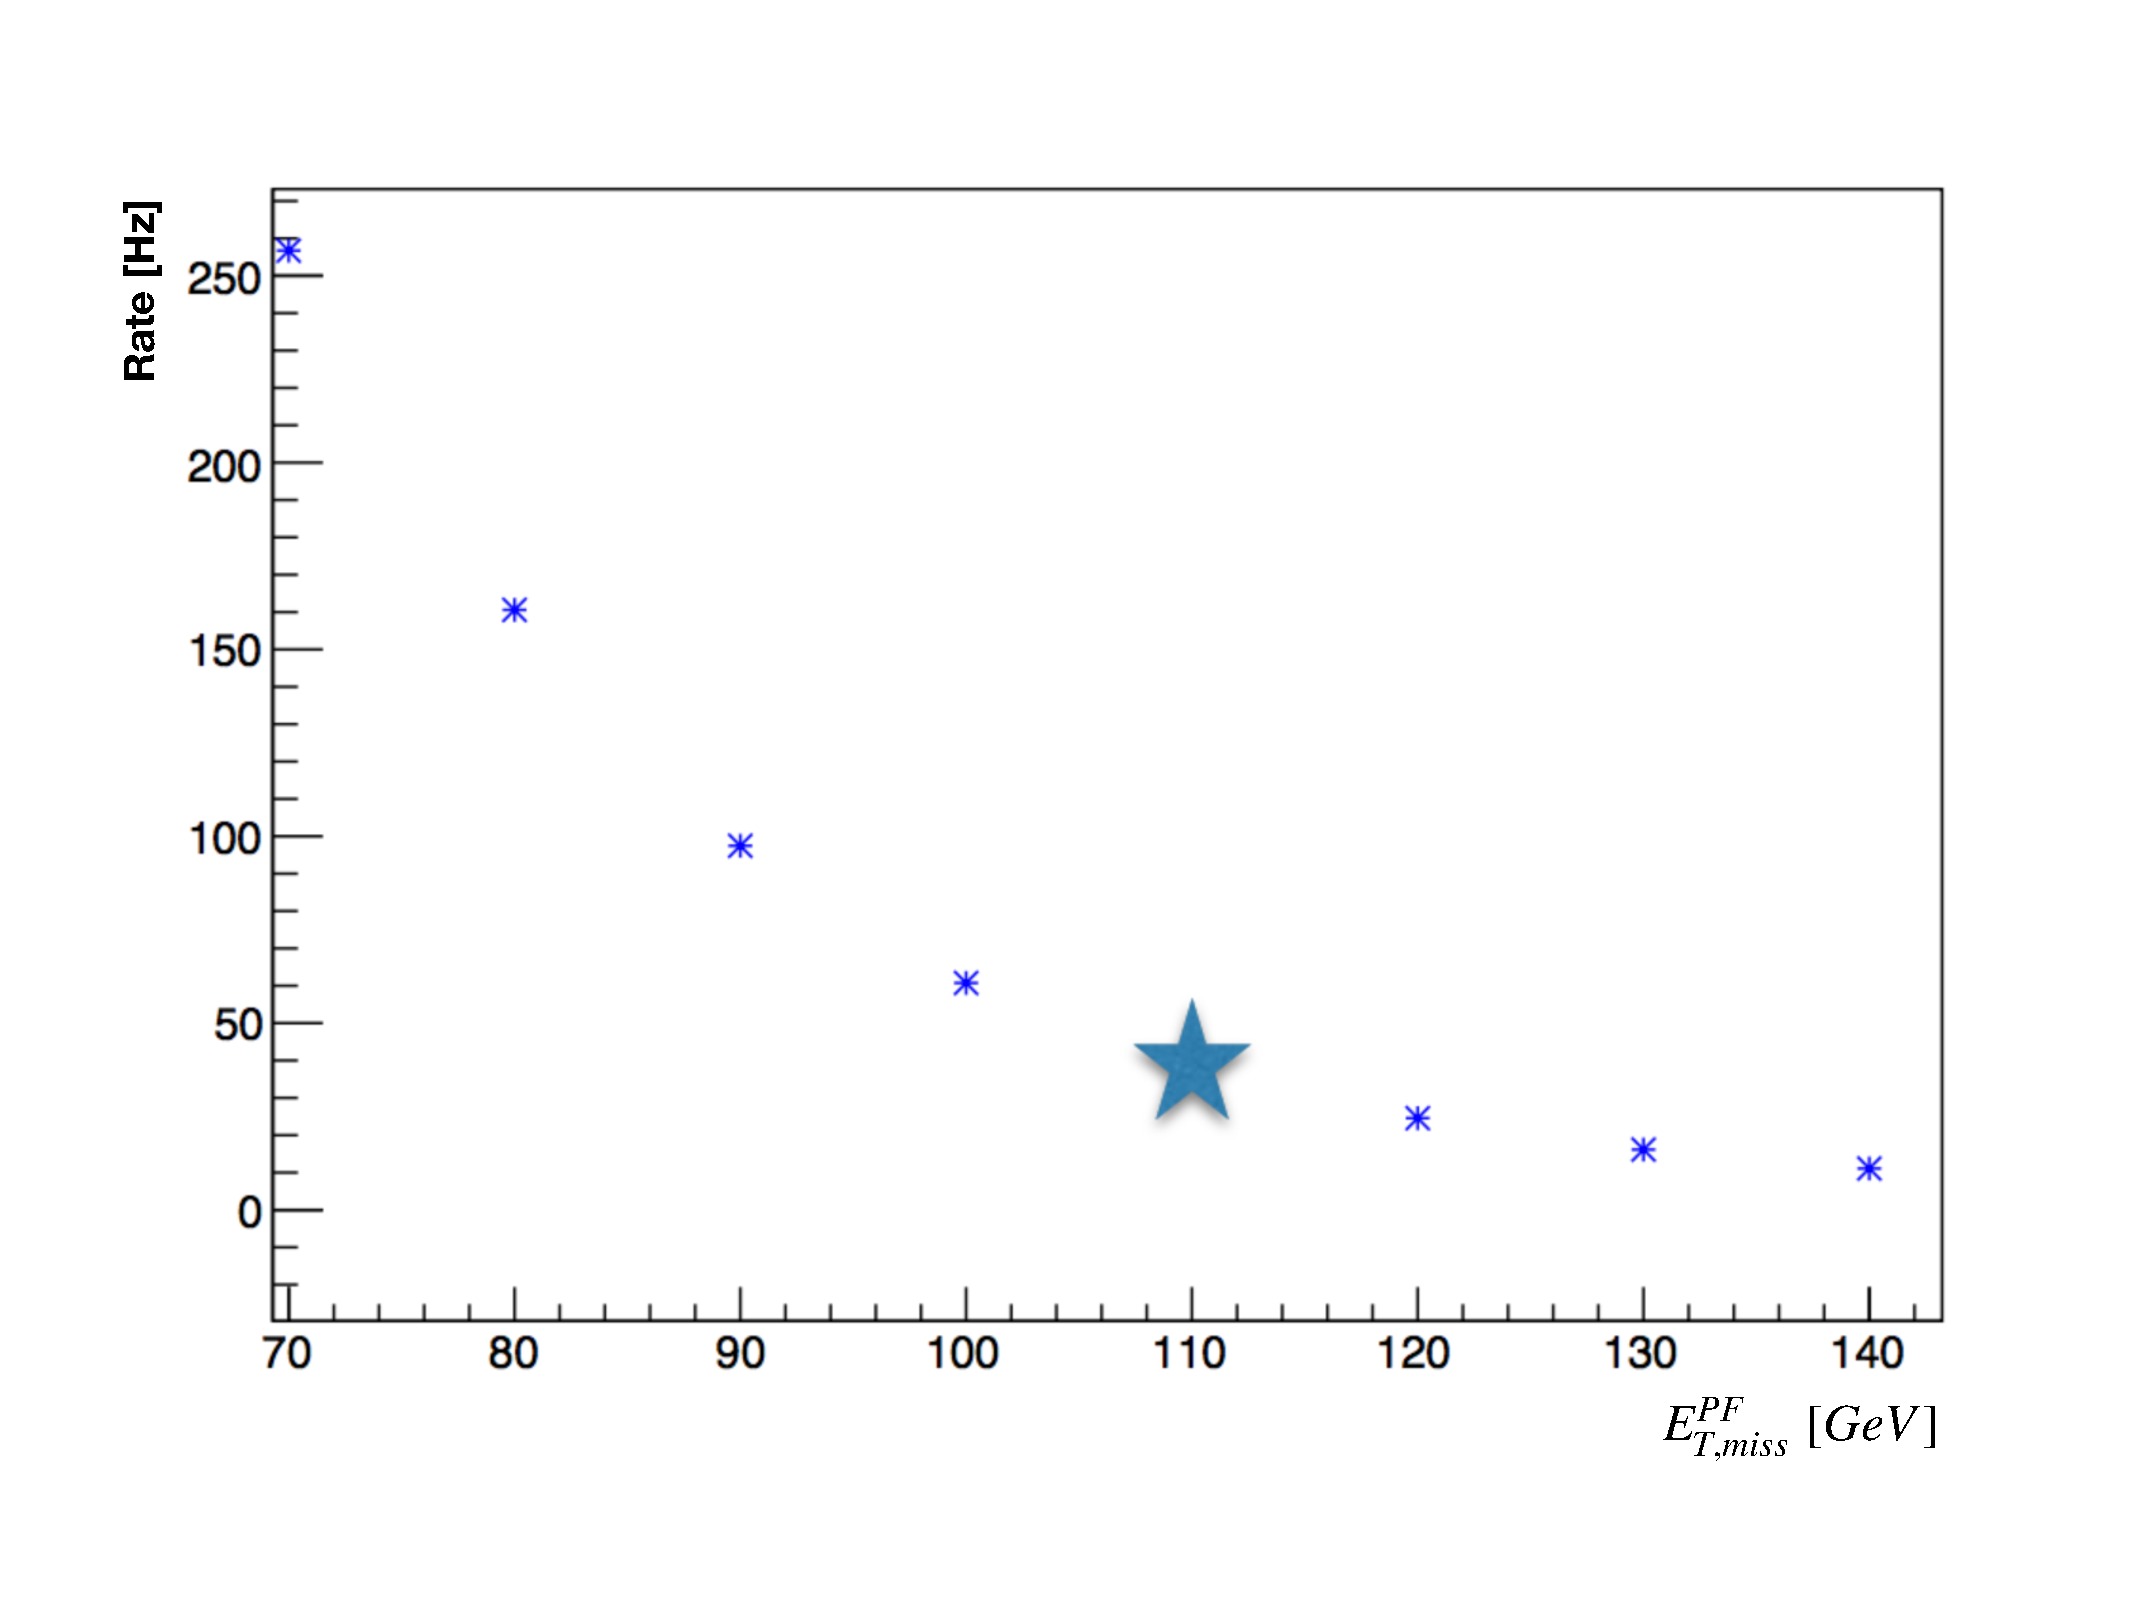
\includegraphics[width=0.75\textwidth]{CMS_experiment/PFMETvsRate.pdf}
  \caption{Estimate of the total rate of the dijet VBF HLT path versus the requirement on the $E_{T,miss}$.}
  \label{fig:PFMETvsRate}
\end{figure}
Potential issues that come with timing are directly related to the usage of the PF algorithm. As it requires the largest amount of time, a requirement was implemented in order to reduce the amount of events that would initialize it and then proceed to be rejected due to the $E^{PF}_{T,miss}>$~110~GeV requirement. This has lead to the inclusion of the $E^{Calo, NC}_{T,miss}$ selection listed above. A correlation study between these two $E_{T,miss}$ variables was performed (as shown in Figure~\ref{fig:VBF_rates_timing}). 
\begin{figure}[!htbp]
  \centering
    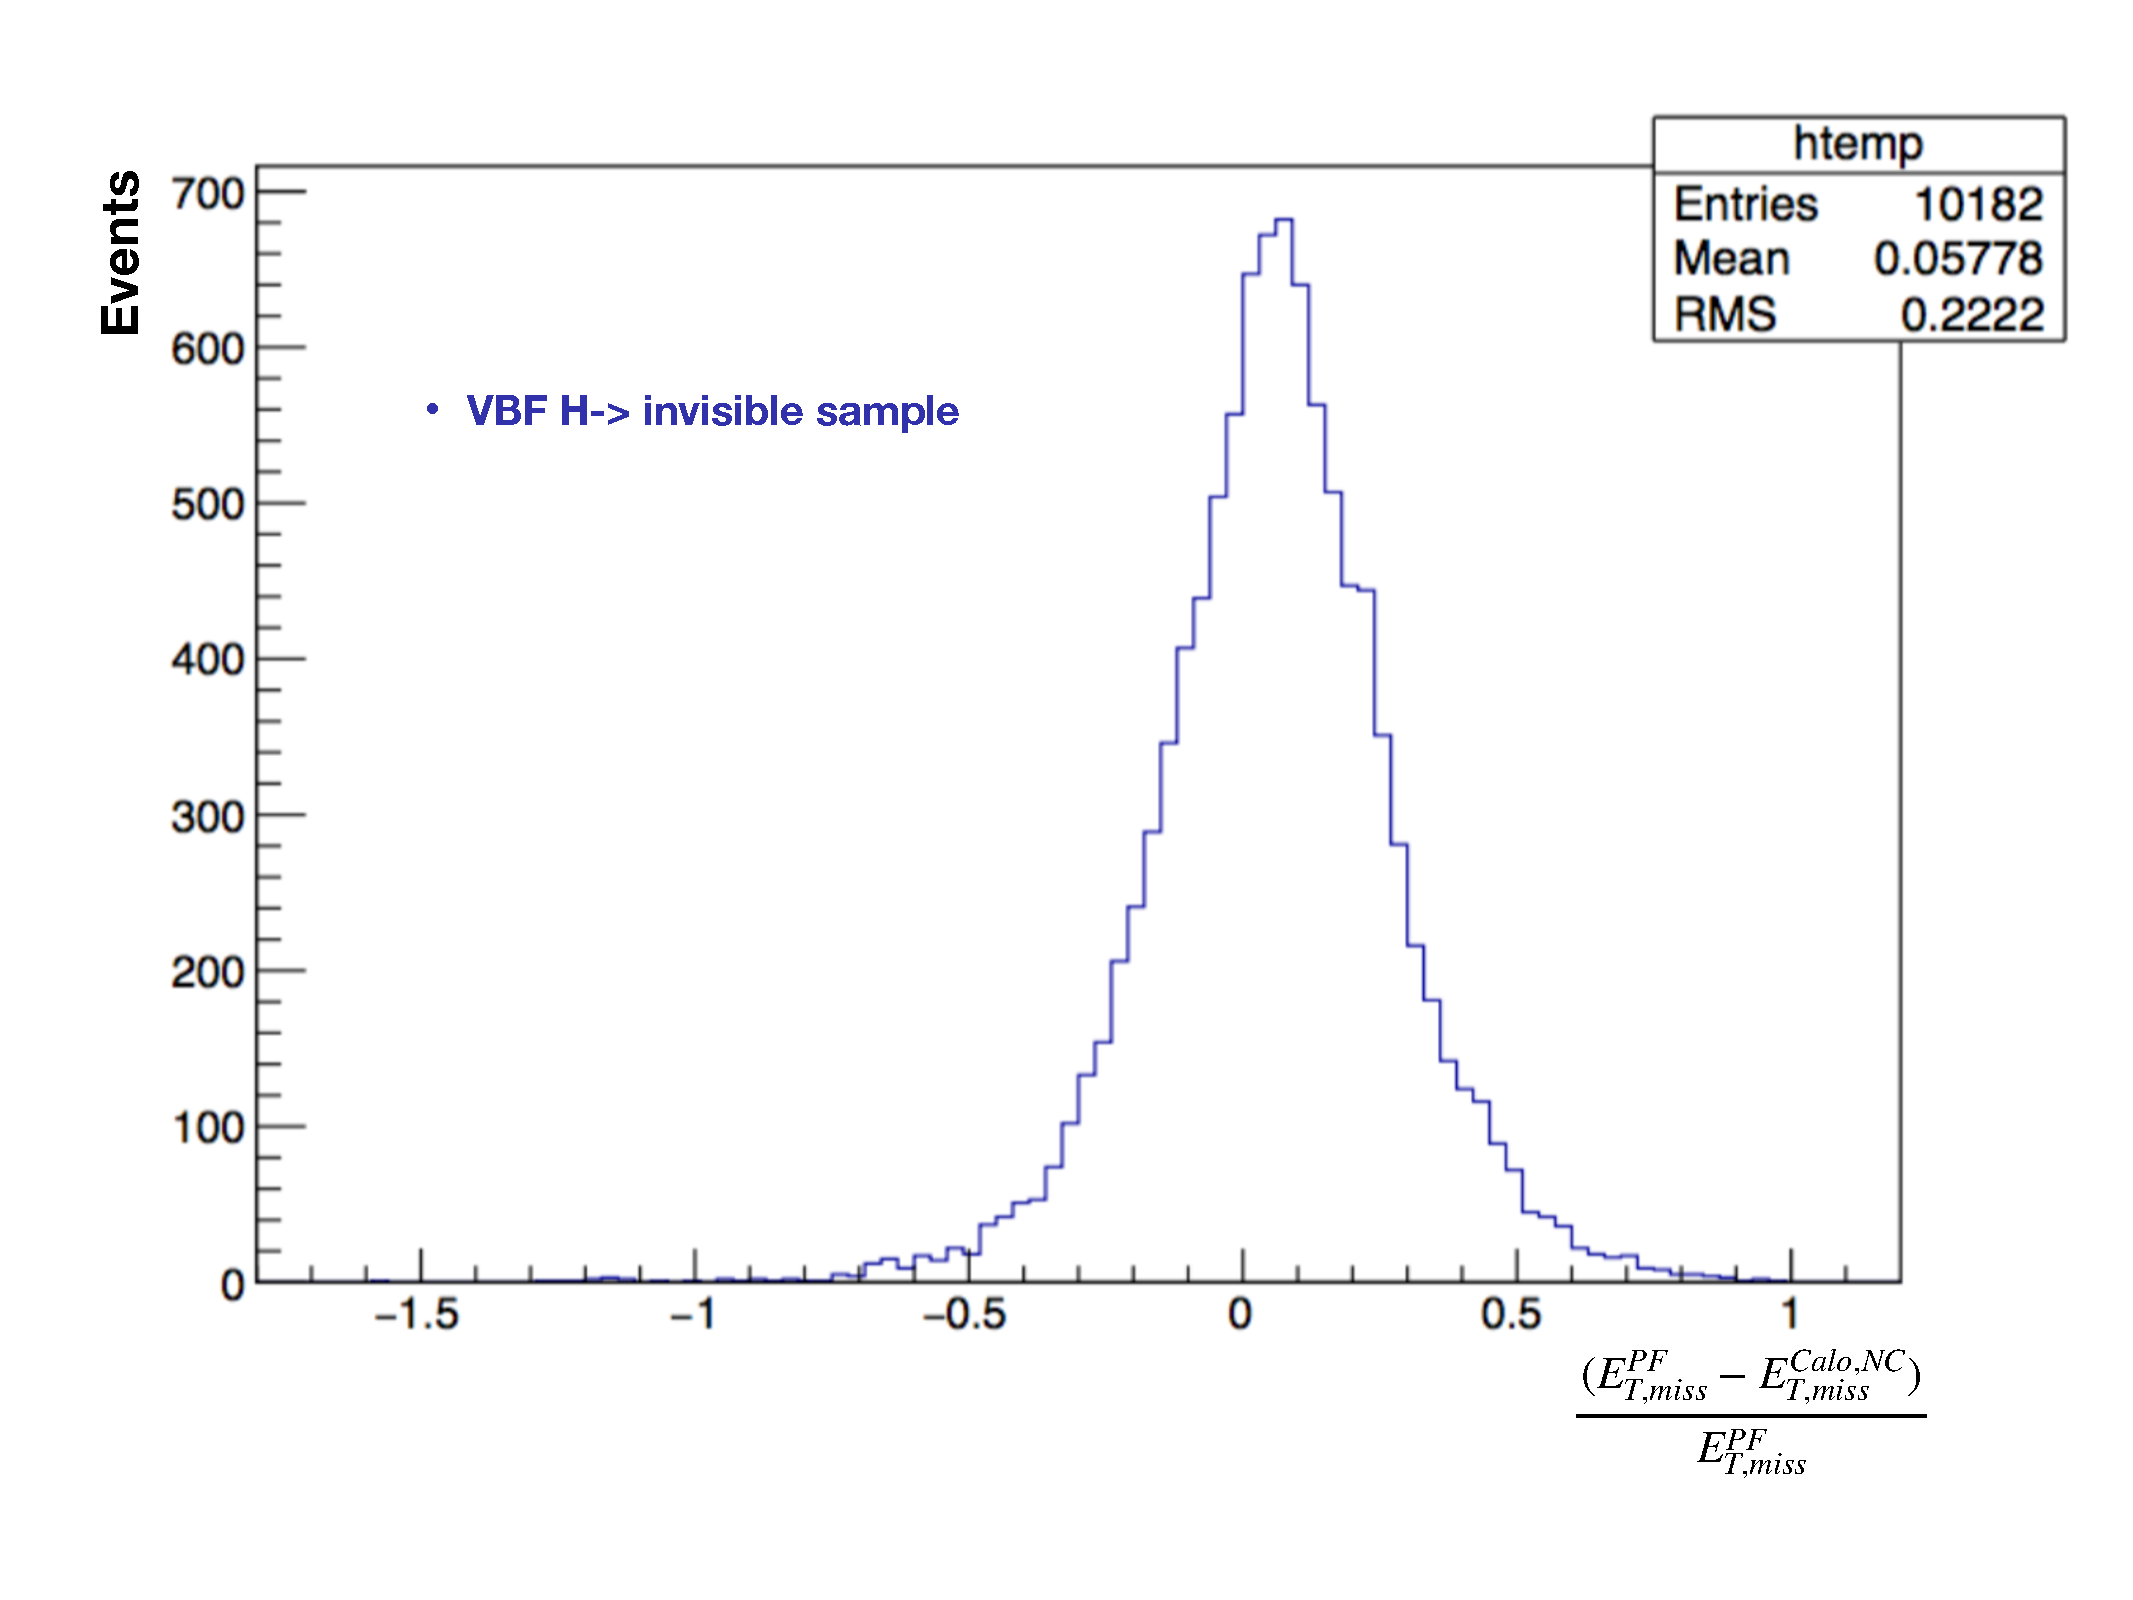
\includegraphics[width=0.75\textwidth]{CMS_experiment/PFvsCaloMET.pdf}
  \caption{Correlation study between the $E^{PF}_{T,miss}$ and $E^{Calo,NC}_{T,miss}$ done using the VBF H$\rightarrow$inv simulation sample.}
  \label{fig:VBF_rates_timing}
\end{figure}
It can be seen that no significant signal loss is expected if a requirement on the $E^{Calo, NC}_{T,miss}$ is imposed to be $\sim$60~\% of the one on the $E^{PF}_{T,miss}$. This, as a result, will stop a large amount of events from reaching modules which call the PF algorithm, instead stopping right after the $E^{Calo, NC}_{T,miss}$ producers, which take a lot less time.

\hspace{10pt} The triple jet path inherits most of the same workflow as its dijet counterpart, differing only in the final choice of jets. This triple jet category is more oriented towards analyses such as the VBF H$\rightarrow$bb$\tau\tau$, where it might bring additional sensitivity. From the perspective of the H$\rightarrow$ inv analysis, this triple jet scenario is valuable as a safeguard option for the subtle differences between the offline and HLT PF jets (which can also be seen by its significantly smaller rate).

\hspace{10pt} These HLT paths were introduced during the 2017 data collection and continued to be used in their original state until the end of the Run 2 phase. The pure and total rate of these paths for the 2018 data taking period are given in Table~\ref{tab:hlt_rates}. Their performance is going to be described in Section~\ref{subsec:vtr_selection}, where it will be shown how they influenced the creation of a new analysis subcategory.

\begin{table}[htbp]
    \centering
    \footnotesize
    \begin{tabular}{llcc}
     Path name & Status &Total Rate [Hz] & Pure Rate [Hz] \\   \hline\hline
           & & & \\
      HLT\_DiJet110\_35\_Mjj650\_PFMET110\_v*   &  signal & 36.88 & 7.84\\
      HLT\_DiJet110\_35\_Mjj650\_PFMET120\_v*   &  backup & 25.81 &  0 \\
      HLT\_DiJet110\_35\_Mjj650\_PFMET130\_v*   &  backup & 18.99 &  0\\
      & & &\\
      HLT\_TripleJet110\_35\_35\_Mjj650\_PFMET110\_v* & signal & 0.91 & 0.44 \\
      HLT\_TripleJet110\_35\_35\_Mjj650\_PFMET120\_v* & backup & 0.44 & 0\\
      HLT\_TripleJet110\_35\_35\_Mjj650\_PFMET130\_v* & backup & 0.25 & 0\\
      & & & \\\hline\hline
    \end{tabular}
    \caption{Measurement of rates for main VBF paths and their backups during 2018 era of data taking.}
    \label{tab:hlt_rates}
\end{table}

\hspace{10pt} As a final remark, it is important to note that even though the matching module had been created for the purposes of the VBF$\rightarrow$inv analysis, it has been used in other studies of the Higgs boson within the CMS experiment, such as the aforementioned $H\rightarrow \tau\tau /~ HH\rightarrow bb\tau\tau$ analyses, helping them to take the advantage of the L1 VBF seed by building their VBF HLT paths.

 



%\section{HLT performance during Run 2}
%\subsection{Introduction}
%\hspace{10pt} Being a general purpose detector, the CMS experiment has a range of dedicated working groups with each being in charge of a particular area of research. In order to efficiently illustrate the performance of the HLT during the Run 2 era, the following paragraphs are going to showcase selected examples of paths within the control of the Higgs Trigger Group. 
%\subsection{Performance of the cross triggers}
%\subsection{Performance of the VBF tau triggers}
%\subsection{Conclusion}


 \tikzset{
    pgfornamentstyle/.style={scale=0.4}
  }
\begin{center}
    \expandafter\pgfornament\expandafter{88}
\end{center}
 \tikzset{
    pgfornamentstyle/.style={scale=1}
  }
\restoregeometry






\newpage
  \newgeometry{left=0cm,bottom=0cm,top=0cm,right=0cm}
  \begin{tikzpicture}[remember picture, overlay]
  \node[inner sep=6pt] (chapter) at (current page.center){\Huge Part III: The study};
  \node[inner sep=12pt, below of=chapter, text width=10cm, align=center, outer sep=12pt] (title1) {\large \textit{``Triput meri, jednom seci."}};
  \node[inner sep=12pt, below of=title1, text width=10cm, align=center, outer sep=12pt] (title) {-- \textup{Serbian proverb} --};
  \node[anchor=north] at (title.south){\pgfornament[width=5cm]{87}};
  \node[anchor=south] at (chapter.north){\pgfornament[width=4cm,symmetry=h]{58}};
  \end{tikzpicture} 
  \addcontentsline{toc}{part}{Part III: The Study}
 \restoregeometry
\newpage





\normallinespacing
\mediumlinespacing

\chapter{Overview}
\label{ch:overview}

\epigraph{\itshape``However beautiful the strategy, you should occasionally look at the results."}{--- \textup{Sir Winston 
Churchill}}

\hspace{10pt} This chapter provides an overview of Part III of this thesis by summarising the core ideas behind the search for the invisible decays of the Higgs boson produced in a VBF event. As introduced in Chapter~\ref{ch:Higgs_LHC_DM}, this study is motivated as the invisible final state represents a highly suppressed scenario from the perspective of the SM, with Br(H$\rightarrow$4$\nu$)~$\sim$~0.1~\%, yielding a conclusion that any deviation from it would be a clear indication of physics beyond the SM.

\hspace{10pt} The main region of interest or the signal region is defined following topological properties of the VBF Higgs boson production, namely its two jet topology and respective characteristics of said jets. One additional factor used to quantify the invisible contribution is the, previously defined, $E_{T,miss}$ variable. The signal region is formed from two analysis categories each built around a set of trigger algorithms. The low $E_{T,miss}$ category will be represented with the VBF triggers introduced in Chapter~\ref{ch:daq}, while the high $E_{T,miss}$ category is connected to the, more generic, $E_{T,miss}$ based triggers. More details about the categorisation are given in Chapter~\ref{ch:an_strategy}, where a detailed discussion of selection requirements for each analysis category is added alongside the performance of the relevant trigger algorithms (whose performance also influences the selection). The structure of the analysis follows a standardised "blinded analysis" approach, where the data events falling under this region are being omitted from the study until the analysis strategy is finalised. 


\hspace{10pt} Contributions of main sources of backgrounds, in this case being the V+jets processes, are constrained through the introduction of four background control regions mimicking the dijet topology of the signal region, but being in a background dominated region with no signal contribution. An example of this would be regions which contain leptons whose invariant mass is found in a narrow, Z boson mass, resonance range (used to constrain Z+jets backgrounds). These regions require a slight redefinition of the $E_{T,miss}$ variable where the leptons forming the region are to be removed from the calculation of the $\vec{p}_{T,miss}$. This is done in order to have the equivalent selection requirement be as close to the signal region as possible. For these, well known lepton-enriched regions, a common conclusion is that the next-to-leading order computations of respective cross sections of SM processes are enough to describe the data. On the other hand, due to the amount of computational power (and time) needed to produce general purpose samples of that precision being extremely large, V+jet backgrounds are simulated using their leading order calculations. In order to account for the difference, a re-weighting procedure alongside with its associated uncertainties is introduced. These higher order corrections are the main focus of Section~\ref{sec:higer_order_corrections}. Lastly, a special attention needs to be given to the estimation of the contribution of QCD multijet processes in the signal region. This procedure involves creation of a dedicated control region largely populated with multijet events by inverting a single requirement from the signal region definition. This approach is needed due to a lack of statistical precision in QCD multijet simulation samples. More details about these dedicated control regions and respective studies are given in Chapter~\ref{ch:control_regions}.

\hspace{10pt} This study focuses on data collected by the CMS experiment during 2017 and 2018 eras of data taking, with the final combination being performed with the study focusing on the 2016 era without re-analysing the data. These eras brought their share of detector problems which were affecting the quality of the collected data, unfortunately, in both years. A common problem is found in the appearance of a data excess in leading/subleading jet $\eta$ distributions in the signal region, which is not well modeled in the simulation. Other important problem happened during the 2018 data taking period, when a part of the HCAL suddenly stopped working leaving a large portion of the data without any HCAL information in the affected region. Both of these problems are addressed in detail and accompanied with respective mitigation approaches in Section~\ref{sec:data_quality}. The signal extraction strategy and the approach used to set the 95~\% CL upper limit on the Br(H$\rightarrow$inv), detailing the connection between the dedicated control regions and the signal region, is the main focus of Chapter~\ref{ch:fit}. A discussion of major sources of uncertainties (both theoretical and experimental) is given, alongside the final results inclusive of the combination with the 2016 study. The conclusion, presented in Chapter~\ref{ch:conclusion}, introduces an approach to combining the results from searches for the invisible state focusing on other production modes through the use of a novel software framework. Lastly, a discussion of the future stages of the LHC from the perspective of this analysis is presented, putting a fitting conclusion to the entire H$\rightarrow$ inv story presented in this thesis.




\newpage
\chapter{Object definitions}
\label{ch:objects}
%\epigraphfontsize{\small\itshape}
\epigraph{\itshape``All compromise is based on give and take, but there can be no give and take on fundamentals. Any compromise on mere fundamentals is a surrender. For it is all give and no take. }{--- \textup{Mahatma Gandhi}}


\section{Introduction}


\hspace{10pt}\lettrine[lines=2]{\initfamily{T}}{he foundation of most experimental studies} is based around the connection between the original idea and the actual reality presented in the form of technical possibilities, in practice more likely limitations, given by the apparatus at hand. The same statement is applicable for the main interest of this thesis. The idea is very appealing on paper (as previously discussed in Chapter~\ref{ch:Higgs_LHC_DM}), there is a production mode with a strong signature and a possible decay that is highly suppressed when looked at from the SM point of view.

\hspace{10pt} From the perspective of the CMS experiment, each analysis needs to be built from the ground up using the same basis - reconstructed physics objects. Following the conclusion that a good way to describe the "invisible" part of an event is through the usage of $E_{T,miss}$ and through its definition in Equation~\ref{for:met}, it can be seen that it takes the collective information from all parts of the detector to quantify the possible invisible contribution. Speaking in technical terms, all available objects will have a role to play in this analysis. This chapter will serves as a summary of the processes and algorithms used in order to reconstruct and define the base objects used in physics analyses.% Taking into account that this study covers different eras of the Run-2 phase of the LHC, each object will be defined separately for every year of data taking to accommodate for different conditions of the CMS detector during where necessary.

\section{Particle Flow reconstruction}
\label{sec:particle_flow}
\hspace{10pt} With the limitations imposed by a large stream of events being removed through the usage of a two level triggering system, more detailed reconstruction can be used for the full (offline) reconstruction of physics objects. The PF algorithm~\cite{Particle_flow,CMS-PAS-PFT-09-001,PF:Florian} provides a valuable tool that connects information originating from all detector subsystems in order to provide the most detailed overview of the event possible. It relies on the features of the CMS detector to deliver exceptional tracking performance which is then combined with the information coming from calorimeters and muon detectors. The idea of combining calorimeter crystals into TTs replaced with the plan to identify, as precisely as possible, all stable particles originating from collision interactions, hence giving rise to PF candidates. The subsequent grouping of those PF candidates and performing identification techniques, as well as energy sum computations, provides analysers with a set of object collections on which to build their analysis on.


\hspace{10pt} In order to efficiently present object collections vital to the main study of this thesis, each of the following sections will provide a brief overview of the reconstruction techniques used to define a particle collection. This description will be followed by a set of recommendations given by the corresponding CMS Physics Object Group (POG), which are then used to create separate collections for a particle type used further down the analysis chain (i.e. formation of the dedicated control regions etc.).


\subsection{Tracks and primary vertex}
\label{sec:tracking}
\hspace{10pt} The tracker information on charged particles is essential in their further identification and usage. The tracker also imposes itself as a better solution when measuring the momenta of charged hadrons than calorimeters (due to the energy loss in material before reaching them) with the added bonus of being able to pinpoint the original directions of particles before being affected by the magnetic field. This all indicates that the preferred course of action is to have the tracking efficiency being as high as possible~\cite{PF:track}. In order to achieve that, an iterative approach is deployed.

\hspace{10pt} A set of tightly tailored requirements is imposed in order to select a first set of tracks. This ensures the purity of track through the removal of fake contributions. The downside of this choice, the lack of high efficiency in track reconstruction, can be eliminated with next steps. The preparation for the second iteration sees the removal of high purity tracks selected in the first step while partially loosening the tight restrictions imposed on track candidates. This approach yields an increase in efficiency while keeping the high purity of selected tracks. A slight change in the approach is introduced after the third iteration. The last two iteration steps are responsible for covering particles originating from secondary vertices, which is being enabled through a modification of requirements regarding the track's origin.

\hspace{10pt} Finally, in order to conclude this discussion, a choice of a primary vertex needs to be made. This is done by looking at the sum of $p_T^2$, where the sum goes over all reconstructed tracks. The vertex with the largest value is chosen to be the primary vertex for the event.

\subsection{Muons}
\label{subsec:muons}
%The basis used to define muons is the \emph{Muon} collection obtained from the nanoAOD trees. As with the \emph{Electron} objects, this collection is centrally produced.

\hspace{10pt} The easiest way to start discussing the definition of muons is to take a look at the criteria helping with the definition of loose muon objects (in further text referred to as Loose Muon ID). This categorisation is important in order to increase the purity of muon objects through the removal of contributions originating from charged hadrons. When applied to a PF object%~\footnote{In this case "Reco Muons", which can contain additional contributions arising from charged hadrons that have beed missed in the identification process}
, the Loose Muon ID requires fulfilment of a few quality conditions. First, the object being looked at needs to be reconstructed as a PF Muon, accompanied by a supplementary condition that this PF Muon candidate needs to be defined either as a Global or a Tracker Muon~\cite{paper:pf_muon_1,paper:pf_muon_2}. 

\hspace{10pt} Both of the aforementioned requirements look for the scenario where the information about the muon candidate's track (originating from the muon subsystems) has been matched to its tracker counterpart. For the Global Muon criteria, tracks originating from two centres of information are extrapolated onto the same plane, upon which respective companions are being selected (one from each set). From there, a global track is extracted via a combined, Kalman-filter approach~\cite{pf:kalman}, fit using the information coming from, previously paired, tracks. The Tracker Muon criteria takes a slightly different approach. It considers all particles which pass very loose conditions\footnote{$p_T>$0.5~GeV and $p>$2.5~GeV} and extrapolates their tracks to the muon detectors while taking into account detector effects. If a hit in muon detectors can be associated with one of these tracks, the PF candidate is considered to be a Tracker Muon.

\hspace{10pt} Following the blueprint instructed by the Muon POG~\cite{muon_pog_1}, the definition of a tight muon objects imposes a stricter requirement on candidates by requiring the object to be a Global Muon with additional quality requirements (in further text referred to as Tight Muon ID). The first pair of quality requirements asks for a goodness of fit for the global muon track be expressed through $\chi^2/N_{DoF}<$~10 and the inclusion of at least one muon chamber hit (with there being at least two) in the aforementioned fit in order to suppress the fake contribution. Further suppression of these effects is enabled through the usage of $d_{xy}<$~2~mm, $d_z<$~5~mm~\footnote{Representing the transverse impact parameter and the z-axis distance of the track when taking the primary vertex as the point of origin} and $N^{hits}_{pixel}>$~0. Finally, in order to achieve an accurate measurement of muon $p_T$, a $N_{tracker}^{hits}>$~5 requirement is imposed. 

\hspace{10pt} Speaking in terms of the analysis level objects, previously defined Loose and Tight Muon ID criteria are combined with additional kinematic ($p_T>$~10/20~GeV), geometric ($|\eta|<$~2.4) and isolation ($\text{I}_{\Delta R<0.4}^{Rel.}<$~0.25/0.15\footnote{The relative isolation variable is defined as the ratio of the sum of $E_T$ of photons and $p_T$ of charged hadrons with respect to the muon candidate's $p_T$ (where the sum covers particle candidates over the area of $\Delta R<0.4$).}) requirements in order to form the Loose and Tight Muon collections (respectively). Figure~\ref{fig:obj_muon} shows the performance of this approach through a comparison of muon properties between data and simulated events. The information is presented after applying the selection requirements used to define the single muon control region for the VBF H$\rightarrow$inv analysis. These are defined in Chapter~\ref{ch:control_regions} and are used to define a VBF-like region dominated by W+jets SM processes. The overall data to simulation comparison for the chosen muon variables shows a generally good agreement. The small discrepancies seen in the high muon $p_{T}$ and $|\eta|$ ranges are covered by the associated uncertainties not shown in the comparison (uncertainty on the simulation samples shows the statistical uncertainty only). More general detector performance studies for the Run 2 phase of data collection can be found in Refs.~\cite{dps:muon_id,dps:muon_rec} showing the performance of the muon reconstruction and identification/isolation, respectively.
\begin{figure}[htbp]
    \begin{center}
        \subfigure[$p_{T,\mu}$]{
        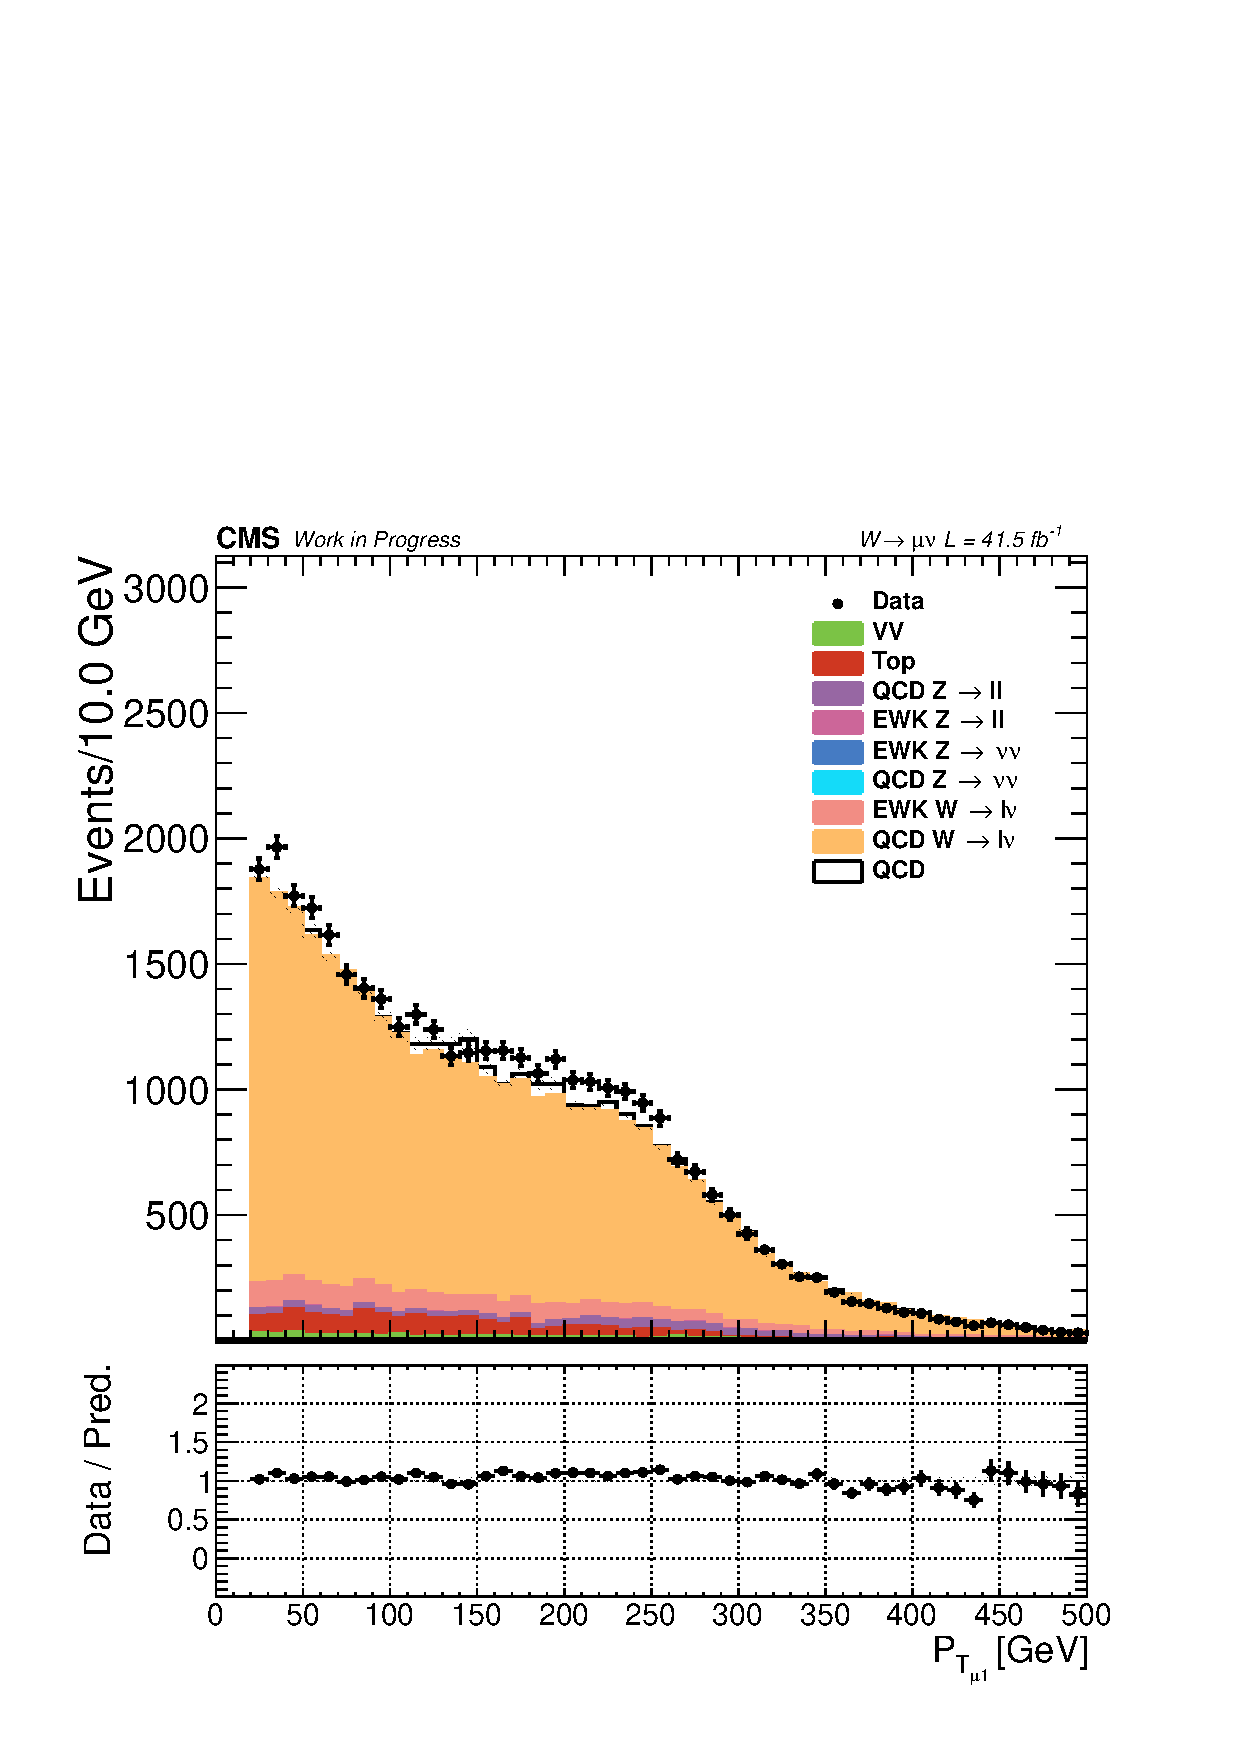
\includegraphics[width=0.49\textwidth]{Control_Regions/2017_MTR/Wmunu/Leading_muon_pt.pdf}}
        \subfigure[$\eta_{\mu}$]{
        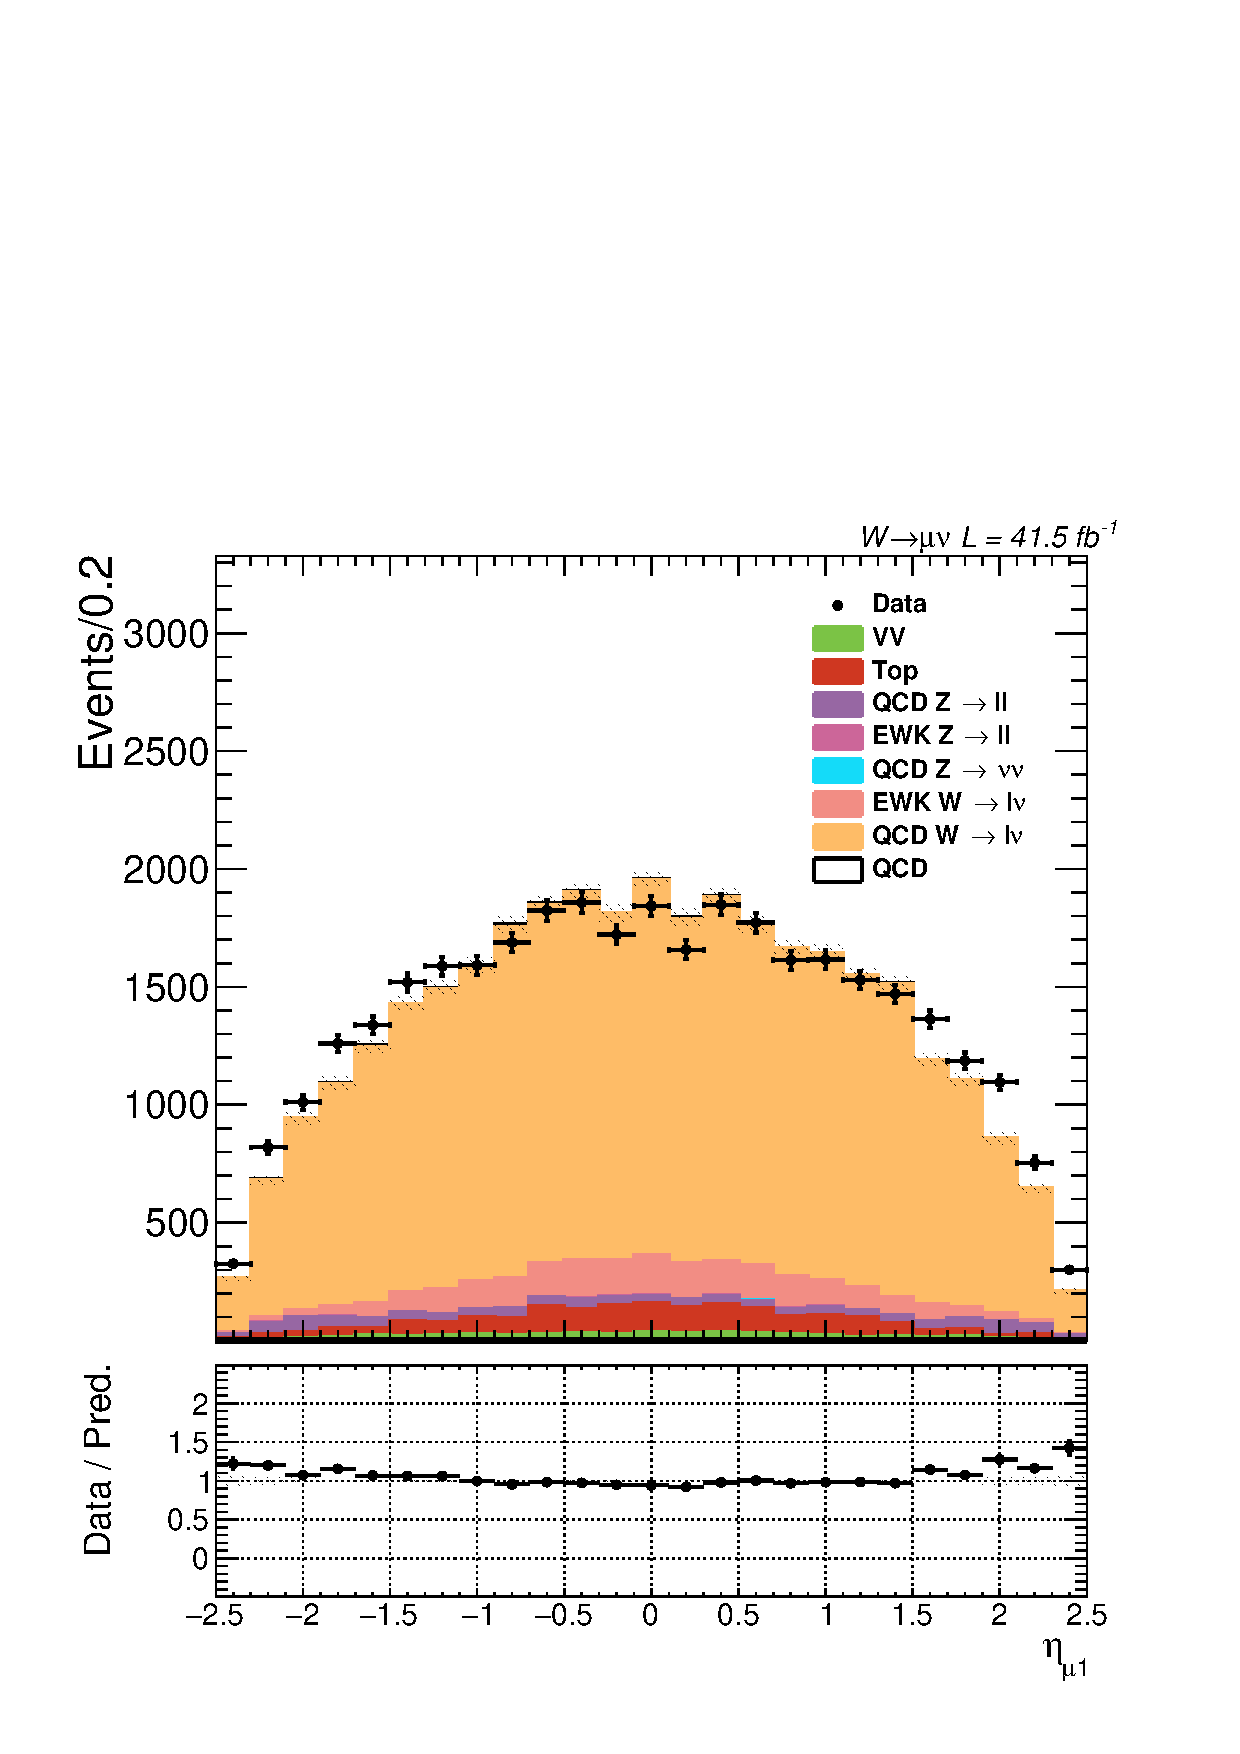
\includegraphics[width=0.49\textwidth]{Control_Regions/2017_MTR/Wmunu/Leading_muon_eta.pdf}}
        \caption{Data to simulation comparison of leading tight muon $p_T$ and $\eta$ variables in a muon enriched (single muon) control region for 2017 data.}
        \label{fig:obj_muon}
    \end{center}
  \end{figure}

\subsection{Electrons}
\label{subsec:electrons}
\hspace{10pt} The interaction of electrons with the tracker material can lead to bremsstrahlung radiation manifesting itself in the form of emitted photons. Other detector effects such as the strong magnetic field cause electron energy deposits to be spread out in the $\phi$ range of ECAL~\cite{paper:pf_muon_1,note_ele_reco,twiki_egamma_1}. %Depending on the value of the particle's transverse momenta, two approaches can be taken in order to reconstruct electrons.

\hspace{10pt} Taking a look at the information given by the calorimeter, it can be seen that $\sim$~97~\% of electron's energy (the same statement stands for photons) is deposited in a 5x5 ECAL crystal structure named the supercluster~\cite{twiki_ecal_clustering}. This allows for a matching procedure to be applied, pairing the supercluster to an electron track (obtained through a fit strategy which takes detector effects into account). As the transverse momenta goes down in value, it becomes more difficult to use the aforementioned approach due to the fact that the radii of the curvature of the particle's trajectory gets smaller. This introduces a problem for the supercluser formation as now the photon contribution (originating from bremhsstrahlung) can be much further in $\phi$ than before, asking for a more careful approach using a multivariate estimator in order to discover pure electron tracks (being relevant for values of $p_T<$~10~GeV).

%The importance of electrons is best definition of the Signal Region requires a veto on the electron objects, while the formation of two out of four Control Regions asks for the existence of specific types of electrons in the event.
\hspace{10pt} Following recommendations given by the E/Gamma POG~\cite{twiki_egamma_1,twiki_egamma_2}, definitions of two main electron collections used in this analysis (Veto and Tight) are summarized in Tables~\ref{tab:electronIDb2017} and \ref{tab:electronIDe2017} (in further text referred to as Cut Based ID). Similarly to the previous section, which dealt with the definition of muon collections, when approaching the definition of analysis level electron collections, the POG recommended Veto and Tight ID criteria are combined with kinematic ($p_T>$~10/40~GeV), geometrical ($|\eta|<$~2.5) and impact parameter requirements\footnote{For the barrel section a requirement of $|d_{xy}|<$~0.05 and $d_z<$0.1 is imposed, while the endcap requirement asks for $|d_{xy}|<~$0.1 and $d_z<$~0.2} in order to acquire the final Veto/Tight Electron collection (respectively). Figure~\ref{fig:obj_electron} shows the performance of this approach through a comparison of electron properties between data and simulated events. Similarly to the muon discussion, these distributions display the data to simulation agreement for the purposes of another control region within the VBF H$\rightarrow$inv analysis (also introduced in more detail in Chapter~\ref{ch:control_regions}). This region focuses on the electron final state of the W boson decay and makes the single electron region. The data to simulation comparison shows a good agreement in general, with the discrepancies seen in $|\eta|>$1.5 being covered by the associated uncertainties not shown in these plots (simulation samples are only presented with their statistical uncertainty). A more general summary of the performance of electron reconstruction and identification is presented in Ref.~\cite{dps:ele_perf}.

\begin{table}[h]
\footnotesize
\centering
\begin{tabular}{|l|c|c|}
\hline\hline
Requirement    & Veto  & Tight             \\\hline
full 5x5 $\sigma_{i\eta i\eta}$ &  $< 0.0126$ &   $< 0.0104$    \\
$|\Delta\eta_{\mathrm{In,seed}}|$ & $< 0.00463$ & $< 0.00255$ \\
$|\Delta\phi_{\mathrm{In, seed}}|$ & $< 0.148$ & $< 0.022$ \\
H/E & $<$ 0.05+1.16/$E_{\mathrm{SC}}$+0.0324$\rho$/$E_{\mathrm{SC}}$ & $<$ 0.026+1.15/$E_{\mathrm{SC}}$+0.0324$\rho$/$E_{\mathrm{SC}}$ \\
Rel. Isolation With EA & $<$ 0.198+0.506/$p_T$	& $<$ 0.0287+0.506/$p_T$\\
$|1/\mathrm{E} - 1/\mathrm{p}|$ & $<$ 0.209	& $<$ 0.159\\
Exp. Missing Inner Hits & $\leq$ 2&	 $\leq$ 1\\
Pass conversion veto & yes	& yes \\
\hline\hline
\end{tabular}
\caption{Summary of E/Gamma POG recommendations used to define Veto and Tight electrons in the barrel region ($|i\eta|\leq 1.479$)~\cite{twiki_egamma_1,twiki_egamma_2,note:AN_19_257}. The conventional names $|\Delta\eta_{\mathrm{In,seed}}|$ and $|\Delta\phi_{\mathrm{In,seed}}|$ represent the geometrical distance between the extrapolated electron track and the selected supercluster. The $\sigma_{i\eta i\eta}$ variable is used to quantify the $\eta$ dimension of the supercluser (weighted by its energy). Finally, the H/E variable controls the ratio of HCAL over ECAL contribution.}
\label{tab:electronIDb2017}
\end{table}

\begin{table}[h]
\footnotesize
\centering
\begin{tabular}{|l|c|c|}
\hline\hline
Requirement    & Veto  & Tight             \\\hline
full 5x5 $\sigma_{i\eta i\eta}$ &  $< 0.0457$ &   $< 0.0353$    \\
$|\Delta\eta_{seed}|$ & $< 0.00814$ & $< 0.00501$ \\
$|\Delta\phi_{in}|$ & $< 0.19$ & $< 0.0236$ \\
H/E & $<$ 0.05+2.54/$E_{SC}$+0.183$\rho$/$E_{SC}$ & $<$ 0.0188+2.06/$E_{SC}$+0.183$\rho$/$E_{SC}$ \\
Rel. Isolation With EA & $<$ 0.203+0.963/$p_T$	& $<$ 0.0445+0.963/$p_T$\\
$|$1/E-1/p$|$ & $<$ 0.132	& $<$ 0.0197\\
Exp. Missing Inner Hits & $\leq$ 3&	 $\leq$ 1\\
Pass conversion veto & yes	& yes \\
\hline\hline
\end{tabular}
\caption{Summary of E/Gamma POG recommendations used to define Veto and Tight electrons in the endcap region ($|i\eta|> 1.479$)~\cite{twiki_egamma_1,twiki_egamma_2,note:AN_19_257}. The naming convention used for control variables follows definitions introduced with Table~\ref{tab:electronIDb2017}. }
\label{tab:electronIDe2017}
\end{table}

\begin{figure}[htbp]
    \begin{center}
        \subfigure[$p_{T,e}$]{
        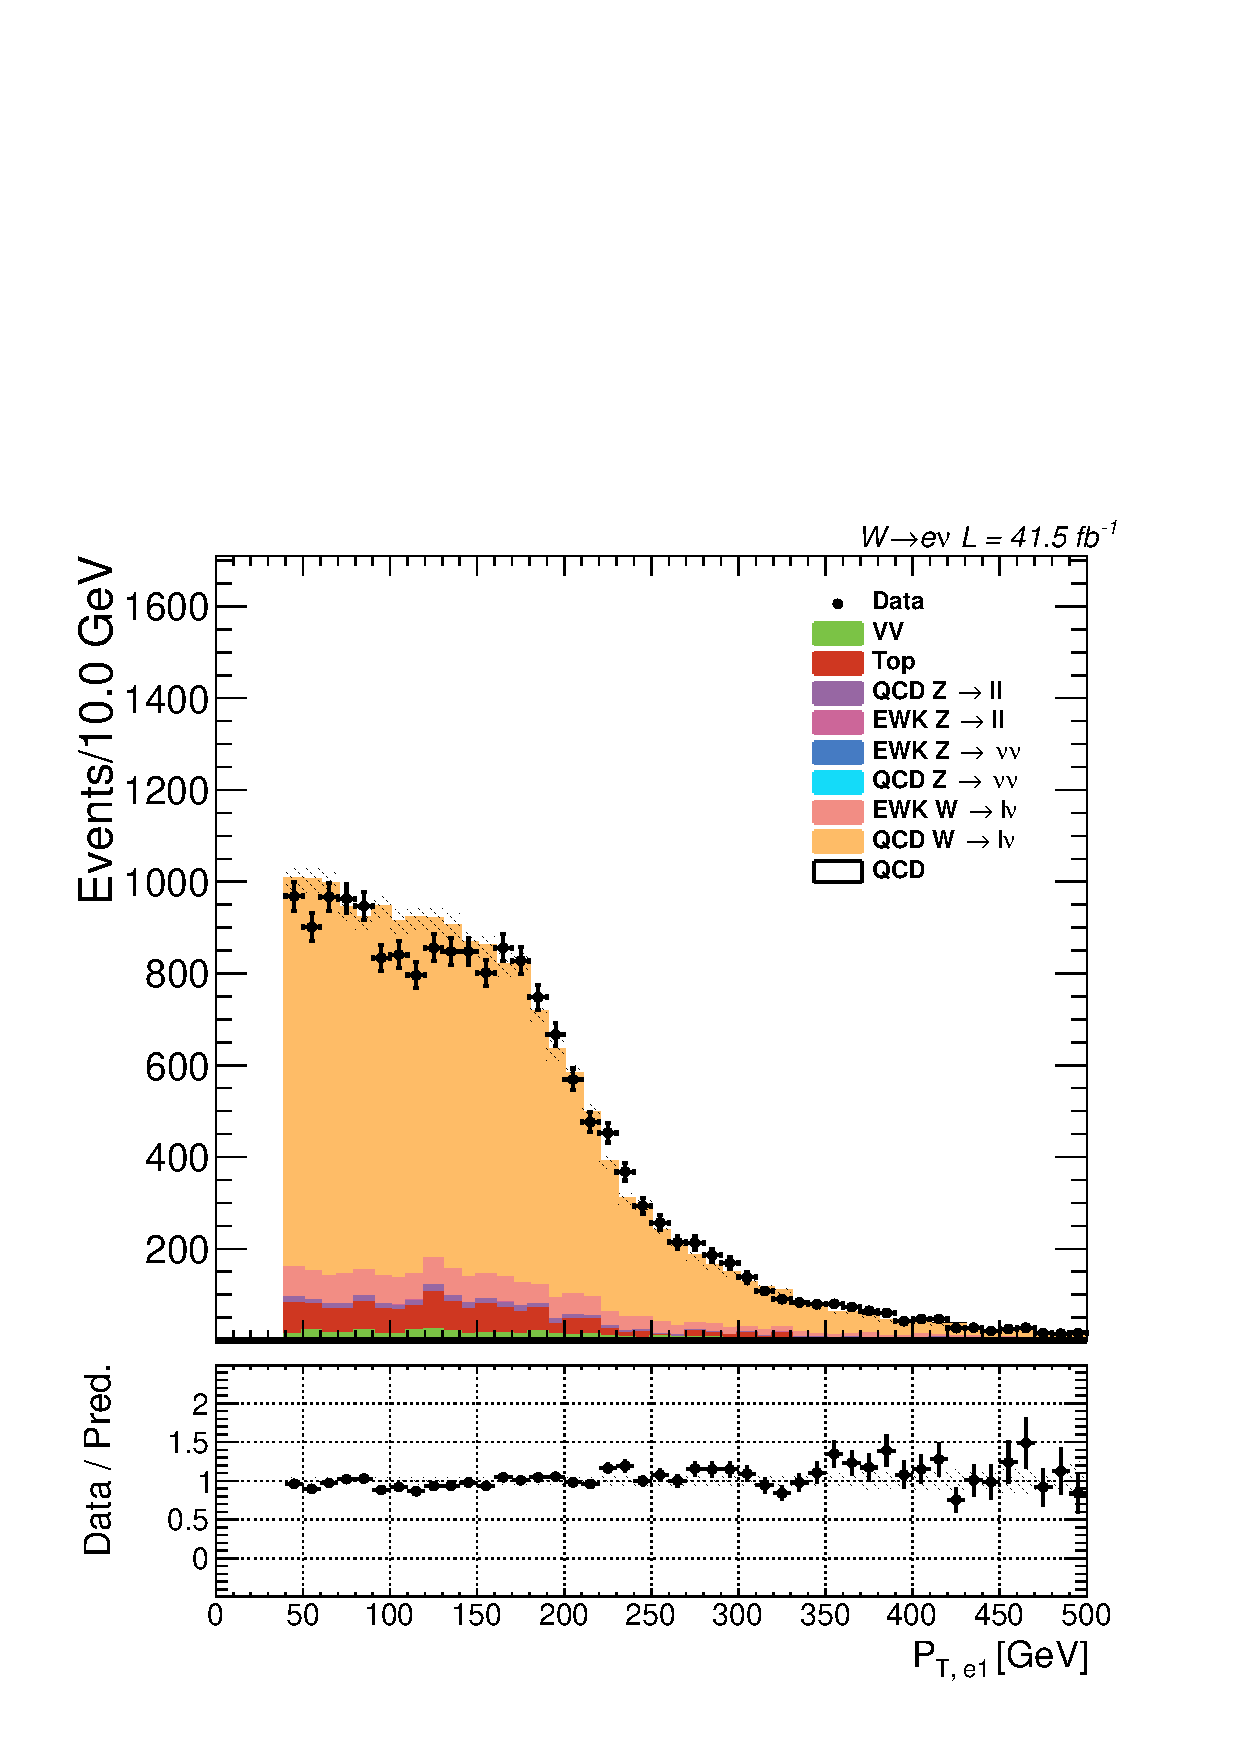
\includegraphics[width=0.49\textwidth]{Control_Regions/2017_MTR/Wenu/Leading_electron_pt.pdf}}
        \subfigure[$\eta_{e}$]{
        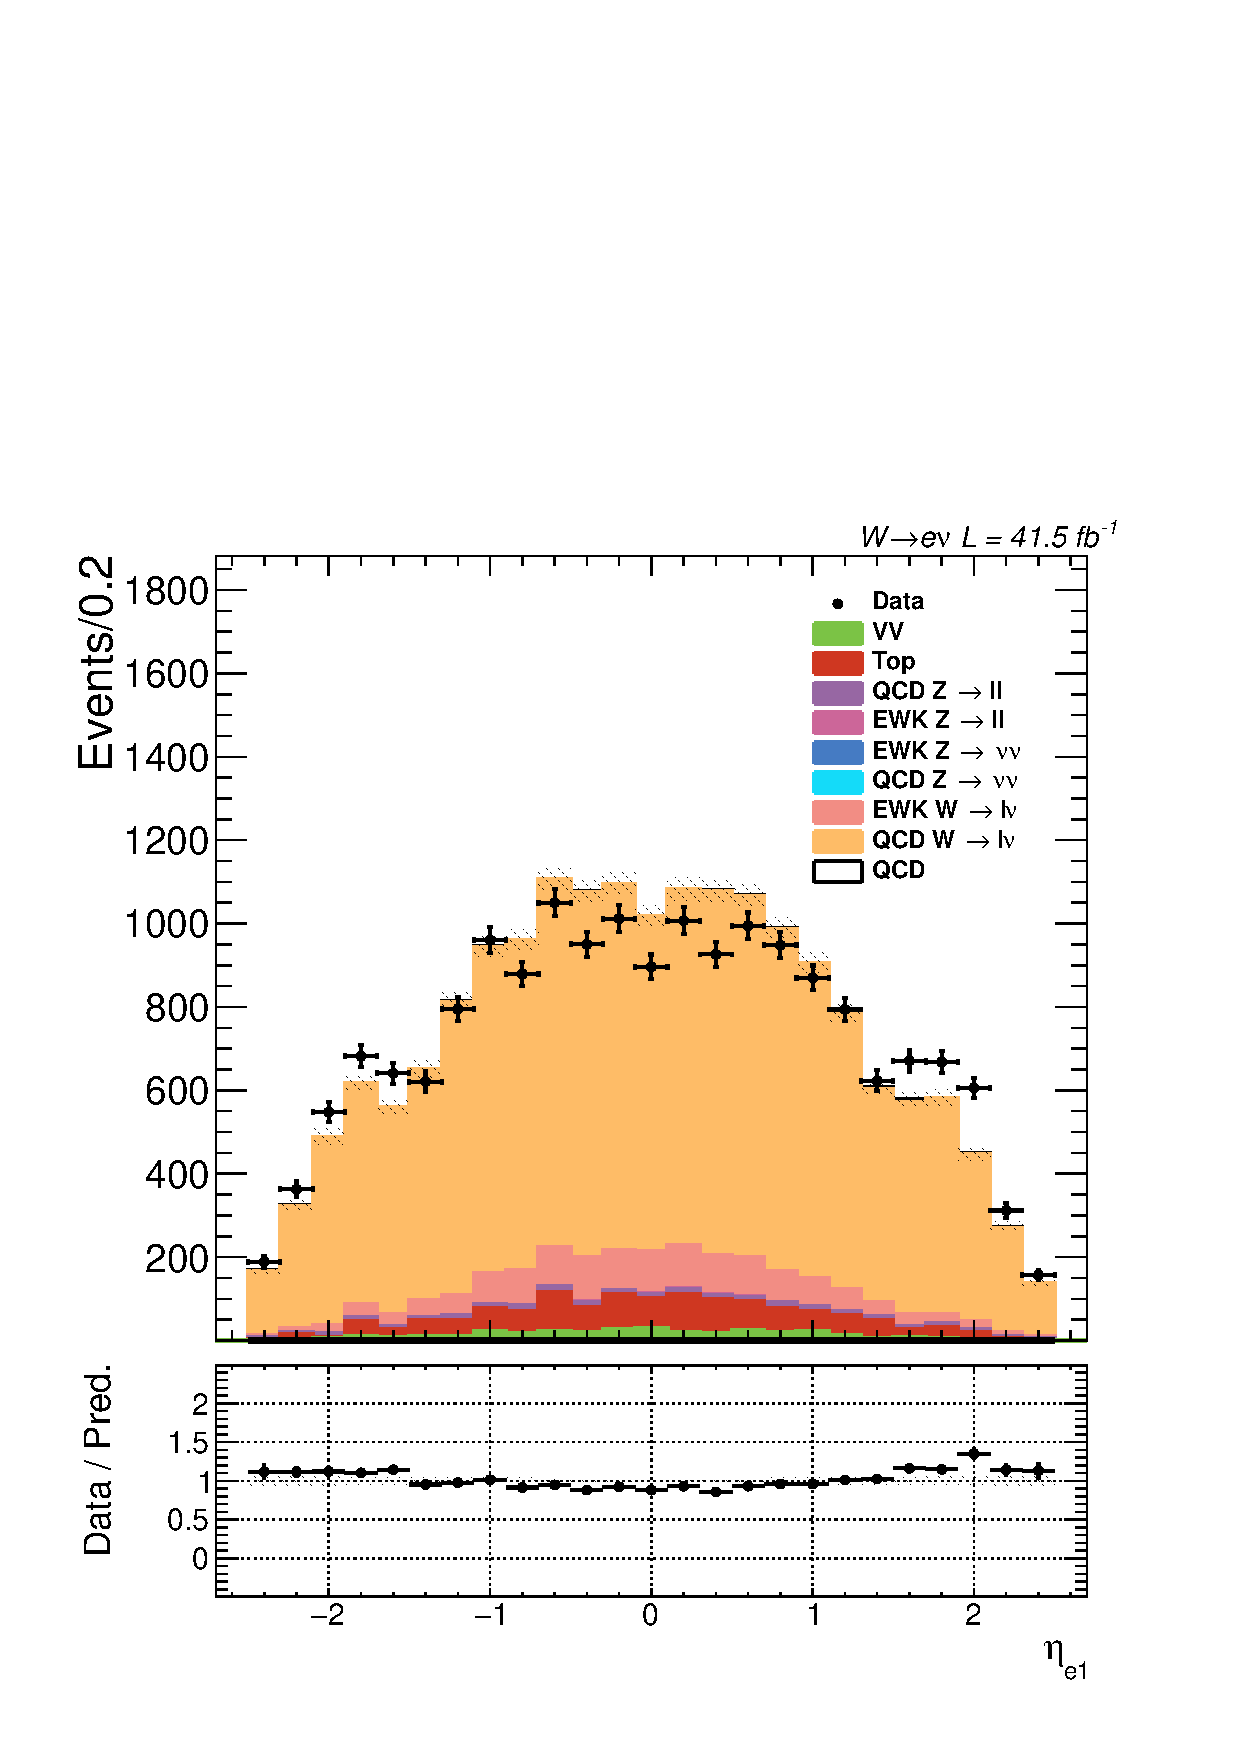
\includegraphics[width=0.49\textwidth]{Control_Regions/2017_MTR/Wenu/Leading_electron_eta.pdf}}
        \caption{Data to simulation comparison of leading tight electron $p_T$ and $\eta$ variables in a electron enriched region for 2017 data.}
        \label{fig:obj_electron}
    \end{center}
  \end{figure}


\subsection{Photons}
\label{subsec:photons}
\hspace{10pt} Staying within the ECAL area of authority, the next item of discussion is the definition of the photon object collection. Upon completing definitions of collections revolving around charged particles and removing their contributions from the ECAL summary, the resulting clusters are used to form photon candidate objects. Further identification of candidates involves using algorithms which vary supercluster dimensions by using a set of predefined shapes associated with a photon deposit~\cite{note:AN_19_257,paper_photon_1} as well as relying on isolation variables. The definition of isolation requirements follows the idea that the scalar sum of transverse momenta of PF candidates (not being associated with the photon candidate's EM shower) is located around a certain geometrical distance from the tested object (in this case $\Delta R<$~0.3).

\hspace{10pt} Being used for vetoing in the process of reducible background rejection, the definition of photons for this analysis involves using objects which pass the Loose photon criteria provided by the E/Gamma POG~\cite{twiki_photon_1} (summarised in Table~\ref{tab:PhotonIDLoose}). Additional kinematic ($p_T>$~15~GeV) and geometric ($|\eta|<~$2.5) requirements are introduced alongside the Photon ID when defining the analysis level collection.


\begin{table}[htb!]
\centering
\footnotesize
%\def\arraystretch{1.2}
\begin{tabular}{l c}
\hline
Variable                                   &  Requirement: Barrel (Endcap)  \\
\hline
\hline
Full 5x5 $\sigma_{i\eta i\eta}$            & $< 0.0106 $ ($< 0.0272 $)    \\
H/E                                        & $<  0.04596 $ ($< 0.0590 $)    \\
charged hadron isolation                   & $< 1.694 $  ($< 2.089 $)     \\
neutral hadron isolation                   & $< 24.032 (19.722) + 0.01512(0.0117)\cdot p_T+2.259(2.3)\times 10^{-5} \cdot {p_T}^2$ \\
photon isolation                           & $< 2.876 (4.162) + 0.004017(0.0037)\cdot p_T$  \\
Conversion safe electron veto              & Yes (Yes)           \\
\hline
\end{tabular}
\caption{Requirements used to define loose photon objects~\cite{note:AN_19_257,twiki_photon_1}.}
\label{tab:PhotonIDLoose}
\end{table}




\subsection{Jets}
\label{sec:jets}
\hspace{10pt} Identification of jets is enabled through the use of the anti-$k_T$ algorithm~\cite{anti_kt}. It produces PF jet candidates which are then used as the basis for creating analysis level jet collections. The aforementioned algorithm, relies on the following properties when defining a jet:
\begin{equation}
    d_{i,B} = \frac{1}{p_{T_i}^2}
\end{equation}
\begin{equation}
    d_{i,j} = min\left (\frac{1}{p_{T_{i}}^2}, \frac{1}{p_{T_{j}}^2}\right )\frac{\Delta R_{i,j}^2}{R^2}
\end{equation}

where $p_{T_{i/j}}$ are transverse momenta of particles $i$ and $j$, $\Delta R_{i,j}$ is the geometrical distance between those particles. The $R$ parameter (taking the value of 0.4 in this scenario) is used as a benchmark jet cone size (similar to the choice of TTs when defining Level-1 jets in Section~\ref{l1:TTs})~\cite{note:AN_19_257}.  

\hspace{10pt} The original idea is, similarly to the Calo jet reconstruction in Chapter~\ref{ch:daq}, to group softer particle candidates around the one which has the largest $p_{T}$  within the area of preference (in this case R$=0.4$). For a hard particle $h$, the algorithm computes both $d_{h,j}$ and $d_{h,B}$ for all soft particles $j$. The soft particle yielding a smallest $d_{h,j}$ is then merged with the hard particle to form a new particle candidate and the process is then re-started from the beginning. The iteration ends when the minimal $d_{h,j}=d_{h,B}$. This leads to the particle $h$, now a combination of the original hard and all soft particles chosen from previous iterations, being defined as a reconstructed jet. Upon removing the newly defined jet from the computation, the algorithms again resets and repeats the procedure until all particle candidates have been assigned to a jet~\cite{Patrick,anti_kt}. This process leads to a set of mostly conically shaped jet objects, with the edge case being represented with a scenario when there are two hard particle candidates within the 2R range. This leads to an overlap (and a slight change in shape) of the reconstructed jet cones created from those candidates.

\hspace{10pt} Comparing the reconstructed jet $p_T$ values between data and simulation leads to the conclusion that the resulting $p_T$ value differs by $\sim 5-10~$\% from the true momenta (where the comparison is inclusive of the full detector acceptance and $p_T$ spectra)~\cite{note:AN_19_257}. Jet objects are corrected for the contribution originating from pile-up through the introduction of an offset in their respective energies. These jet energy corrections are obtained from simulation~\cite{note:AN_19_257,paper_jes_jer,twiki_jes_jer}.

\hspace{10pt} Following recommendations given by the Jet/MET POG~\cite{twiki_jet_met} a set of quality criteria (Jet ID) are added on top of PF jet collection in order to create analysis level objects~\cite{twiki_jet_id}. These involve using a dedicated threshold on the fractions of neutral particles from ECAL and HCAL contributions as well as the muon fraction, number of constituents in a jet object, and the number of neutral particles. This study used the tight Jet ID working point, ensuring identification efficiency of $>99/98~$\% for 2017/2018 eras. Jet ID requirements are supplemented with a requirement of using a medium point of Jet Pile-up ID in order to reject pile-up contributions~\cite{twiki_jet_pileupid}. For the 2017 era of data taking, an additional veto requirement was added for jets within $p_T<$~50~GeV and $2.65<|\eta|<3.139$ range in order to suppress the contribution from jets originating from detector noise~\cite{note:AN_19_257}. This final collection is cleaned from overlap with the lepton and photon collection using a $\Delta R<~$0.4 condition. Figure~\ref{fig:obj_jet} shows the data to simulation agreement for properties relevant to the leading jet from the perspective of the single muon control region for the H$\rightarrow$inv analysis. The general agreement seems to be good across all control regions, with the discrepancies seen in the high $p_{T}$ region of the aforementioned distribution being covered by the associated uncertainty, not shown in this figure. The signal region has a set of jet quality issues mostly plaguing the high jet $|\eta|$ region. Details about these problems and the respective mitigation techniques are summarised in Chapter~\ref{ch:an_strategy}. More general detector performance studies focusing on the jet reconstruction can be found in Ref.~\cite{paper:jet_perf}.

\begin{figure}[htbp]
    \begin{center}
        \subfigure[$p_{T,j}$]{
        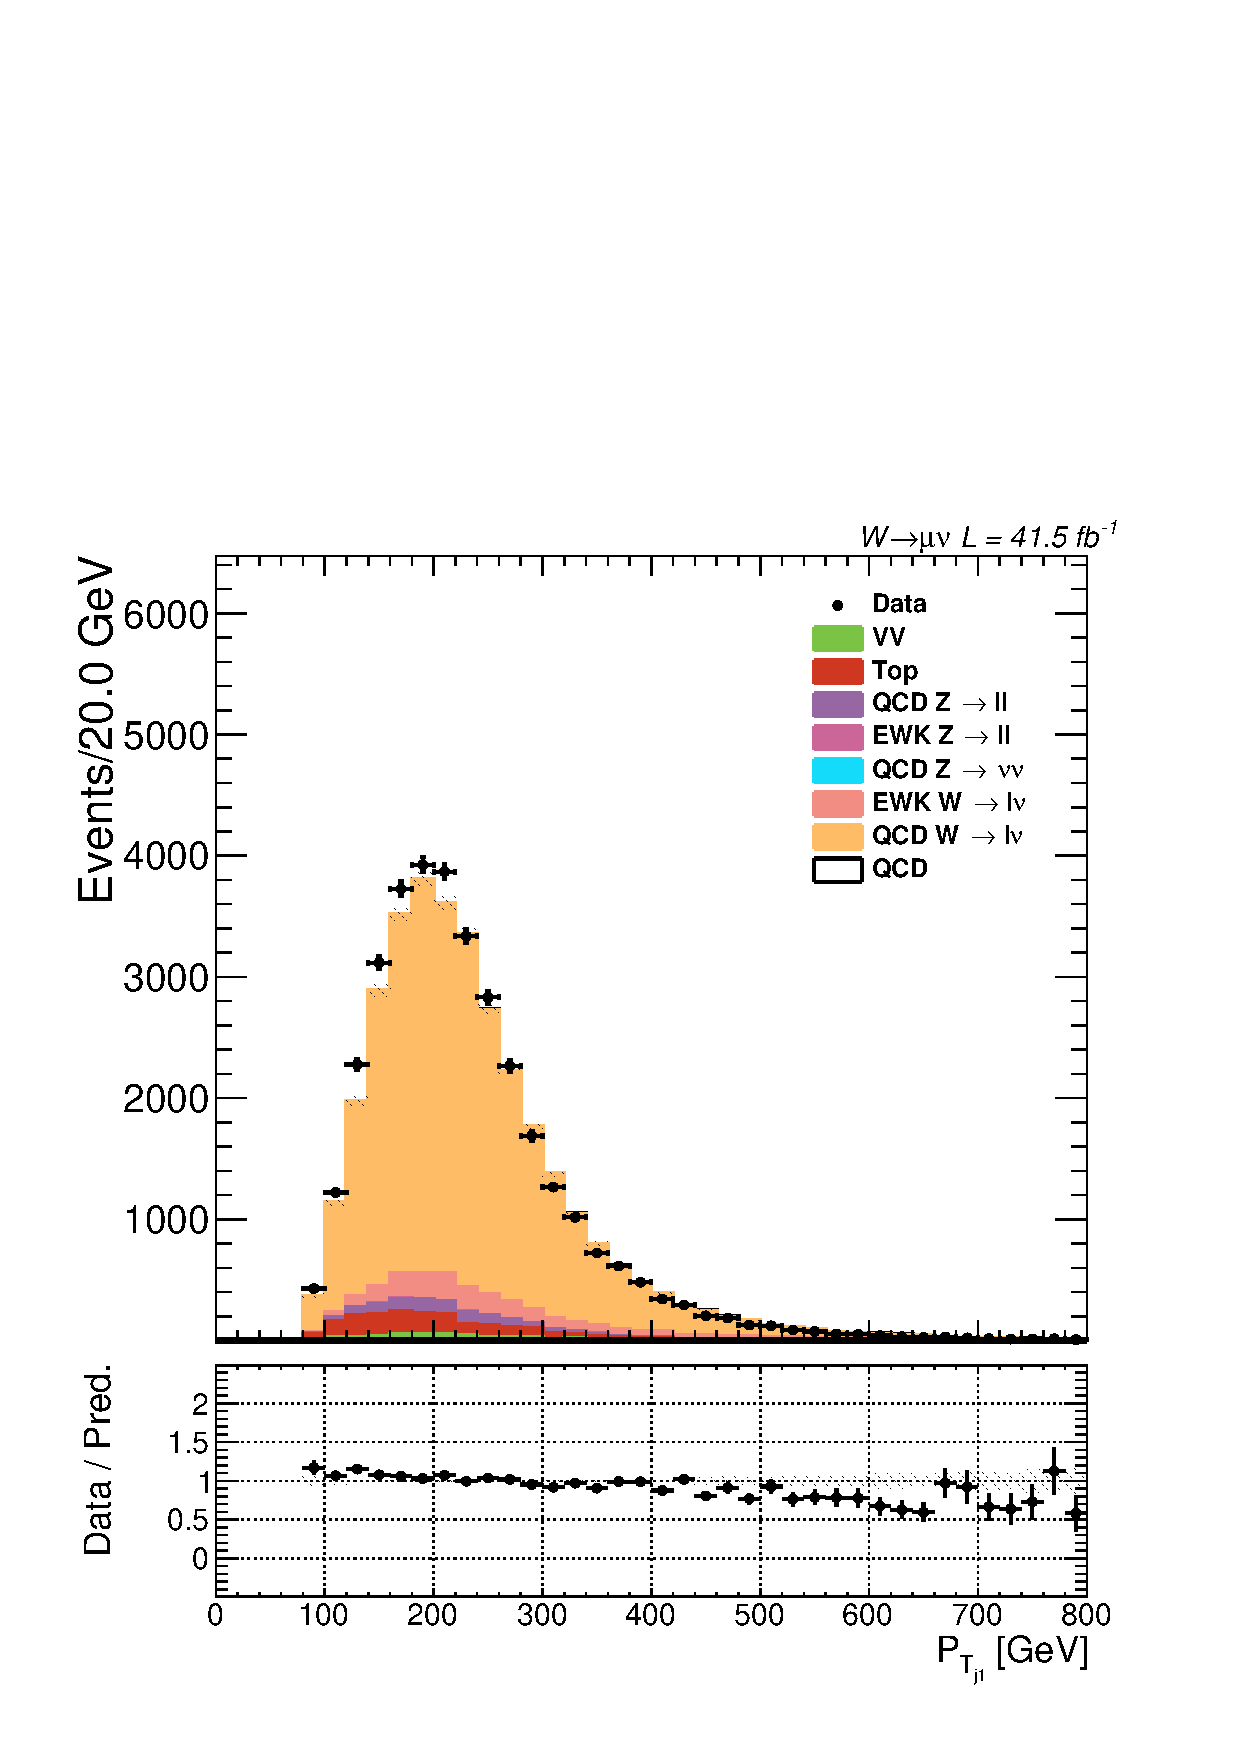
\includegraphics[width=0.49\textwidth]{Control_Regions/2017_MTR/Wmunu/Leading_jet_pt.pdf}}
        \subfigure[$\eta_{j}$]{
        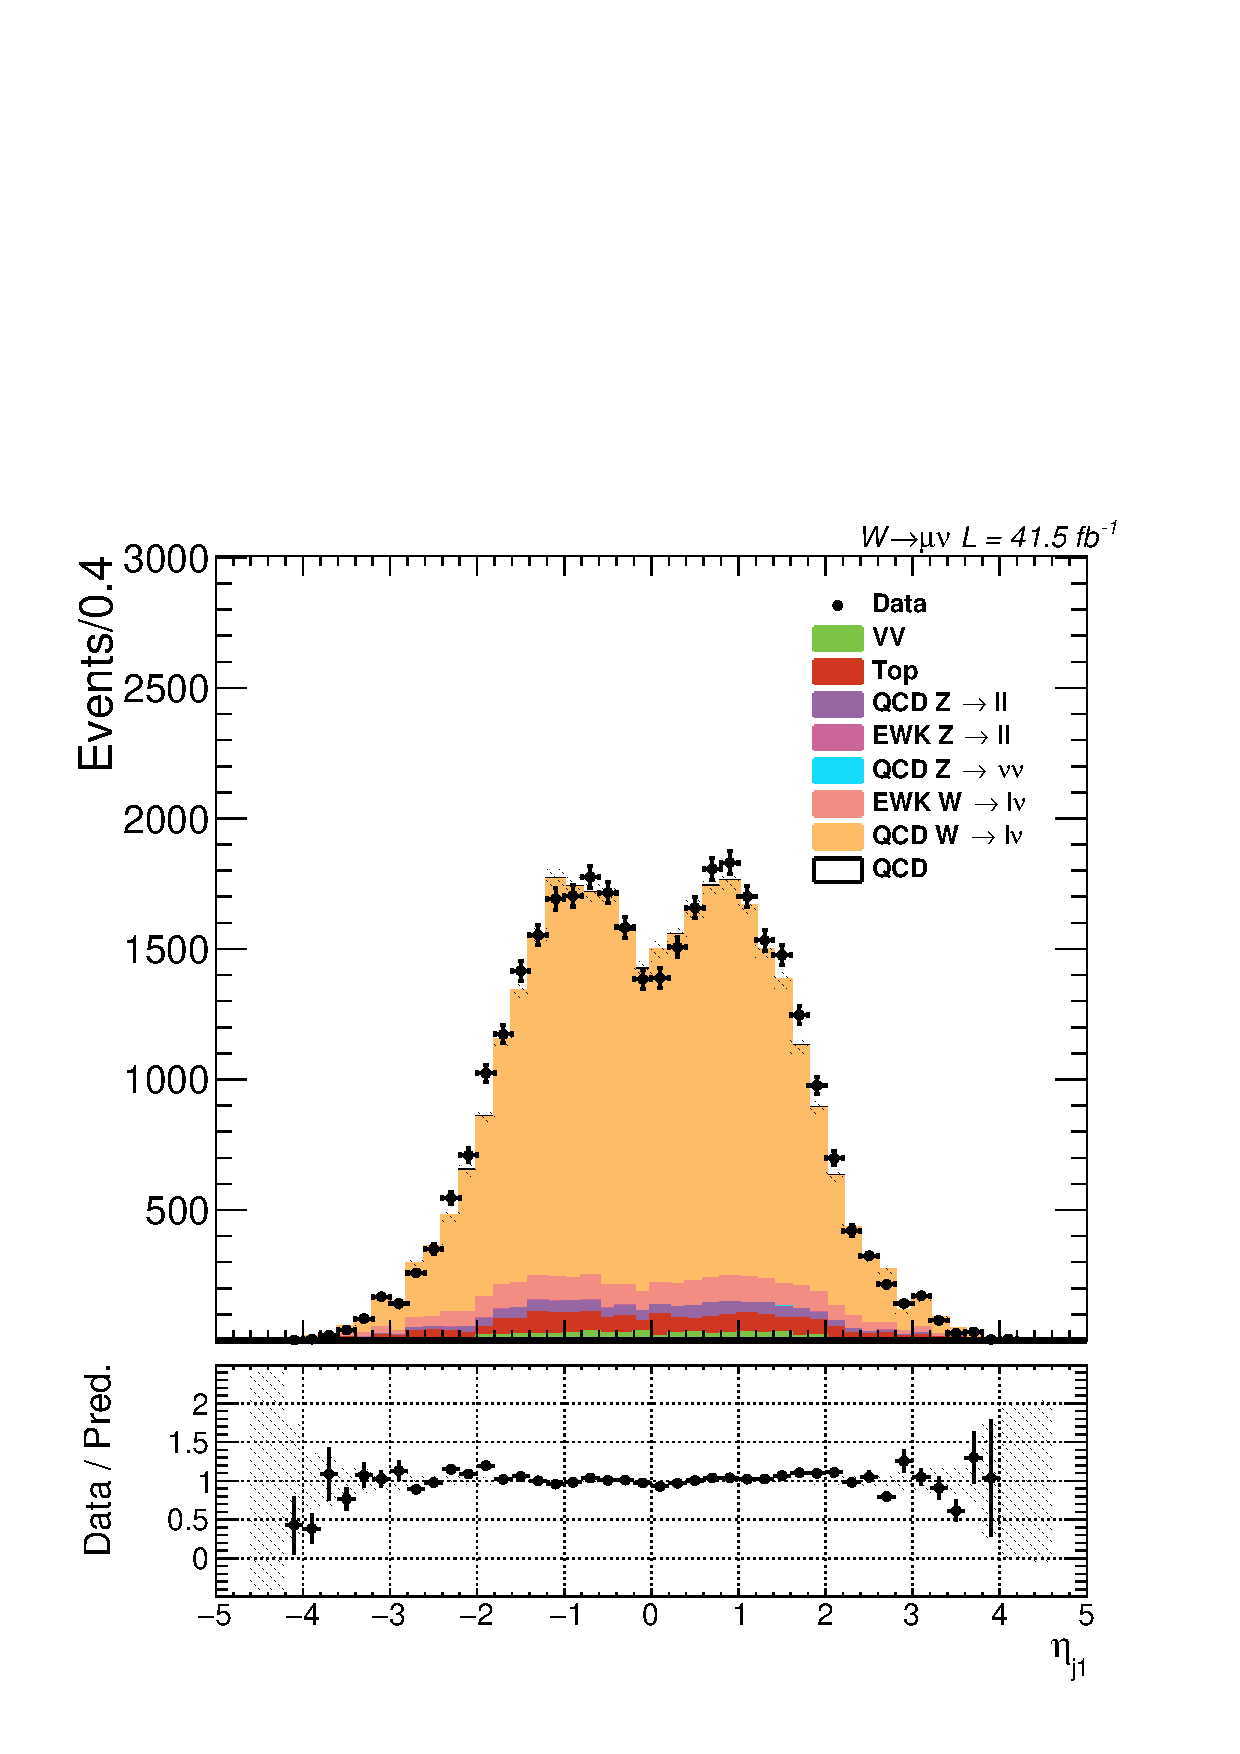
\includegraphics[width=0.49\textwidth]{Control_Regions/2017_MTR/Wmunu/Leading_jet_eta.pdf}}
        \caption{Data to simulation comparison of leading jet $p_T$ and $\eta$ variables in a muon enriched region for 2017 data.}
        \label{fig:obj_jet}
    \end{center}
  \end{figure}




\subsection{B jets}
\hspace{10pt} The definition of b jets\footnote{The b jets or beauty quark jets represent, as the alternative name suggests, jets originating from b quarks.} is important for the control of reducible SM background processes as these objects are used to veto events. This action is closely connected with the contributions originating from top quark processes~\cite{note:AN_19_257}. The POG recommended quality criteria advises the usage of the DeepCSV (Combined Secondary Vertex) tagging algorithm~\cite{paper_deepcsv} with a working point of 0.4941 and 0.4184 for 2017 and 2018 era respectively~\cite{twiki_btag_1}. These numbers correspond to a medium working point of DeepCSV algorithm ensuring an 80~\% efficiency of identifying a b jet. Additional kinematic ($p_T>$~20~GeV) and geometric ($|\eta|<$~2.4) requirements are applied when forming the analysis level object collection.
\subsection{Tau leptons}
\hspace{10pt} Similarly to the previous section, tau objects are important for vetoing events, thus reducing the contribution of V+jets SM backgrounds. A special algorithm is deployed in order to select the hadronically decaying taus\footnote{The final state particles originating from lepton decays of taus are already included in respective muon/electron collections.}. The idea behind the algorithm is to check if the jet object is comprised from objects associated with a tau decay. The selected tau candidates are requested to be completely isolated from other objects (the comparison point for the isolation is $\Delta R<$~0.5/0.3 for 2017/2018 era). Finally, a set of kinematic ($p_T>$~20~GeV) and geometric ($|\eta|<~$2.3) requirements is imposed when creating the analysis level collection~\cite{twiki_tau_pog}.

\subsection{Missing transverse energy}
\label{sec:pf_met_reconstruction}
\hspace{10pt} Defined with Equation~\ref{for:met}, the $E_{T,miss}$ variable provides an important view of the transverse contribution of particles invisible to the detector. From the reconstruction point of view, it is defined through the use of all PF particle candidates by taking a negative vector sum of their corresponding transverse momenta. Following additional corrections changing the jet $p_T$ (previously mentioned in Section~\ref{sec:jets}), a recalculation of the $\vec{p}_{T,miss}$ is performed in order to reflect this change:
\begin{equation}
\vec{p}_{T,miss}(\mathrm{corrected})
=\vec{p}_{T,miss} - \sum_\mathrm{j} (\vec{p}_{T,j}({\mathrm{corrected}})-\vec{p}_{T,j}),
\label{eq:Type1MET}
\end{equation}
%This process of re-evaluating the $E_{T,miss}$ is called the "type-1" correction.
where the sum runs over all jet objects~\cite{note:AN_19_257}. The $p_{T,j}({\mathrm{corrected}})$ tends to form a connection between the PF jet, with momenta $p_{T,j}$, and its real transverse momentum. This corrected transverse momentum is obtained through a set of successive operations, which combined can be illustrated as: $p_{T,j}({\mathrm{corrected}})=\mathcal{C}_{all}\cdot p_{T,j}$ (as presented in more detail in Ref.~\cite{paper:jet_cal}). The first correction forming the $\mathcal{C}_{all}$ is being applied to the PF jet $p_T$ and performs offset corrections which include removal of pile up effects and electronic noise. The newly obtained, offset corrected, momentum is being put through another procedure designed to perform a simulation calibration. It uses the information provided by the simulated samples of well known processes to correct the non-uniformity and non-linearity in jet $\eta$ and $p_T$ respectively. Lastly, the final set of corrections tends to the absolute and relative energy scale calibration, yielding the $p_{T,j}({\mathrm{corrected}})$ used in order to perform the $p_{T,miss}$ recalculation introduced with Equation~\ref{eq:Type1MET}.

\hspace{10pt} Additionally, a set of dedicated filters, listed in Table~\ref{tab:metfilters}, has been implemented by the Jet/MET POG~\cite{twiki_met_filters, note:AN_19_257} in order to mitigate issues of high $E_{T,miss}$ originating from detector problems. They are used to account for contributions arising from detector effects (HCAL/ECAL noise, ECAL calibration, etc.), beam-halo particles and cosmic rays. The procedure follows a simple path, if a filter associates the reconstructed $E_{T,miss}$ to be connected to one of the aforementioned sources, it is marked as being "fake" and the evenr is discarded. These filters are applied as selection requirements at the analysis level.

\hspace{10pt} The performance of this approach is presented in Chapters~\ref{ch:an_strategy} and~\ref{ch:control_regions} for all, VBF H$\rightarrow$inv analysis relevant, regions. A summary of the performance of $E_{T,miss}$ reconstruction is given in Ref.\cite{paper:met_performance,paper:met_performance_run2}~\footnote{These studies are basing their measurements around processes which are well known and do not contain real $E_{T,miss}$. These includes final states such as Z$\rightarrow e^{+}e^{-}$ and Z$\rightarrow \mu^{+}\mu^{-}$.}.
\begin{table}[ht!]
    \centering
    \begin{tabular}{l  c }
        Filter description                                                   & Applied in data (simulation)     \\\hline
        Primary vertex filter                                      & \checkmark  (\checkmark) \\
        Beam halo filter                                           & \checkmark  (\checkmark) \\
        HBHE noise filter                                          & \checkmark  (\checkmark) \\
        HBHEiso noise filter                                       & \checkmark  (\checkmark) \\
        ECAL TP filter                                             & \checkmark  (\checkmark) \\
        Bad PF Muon filter                                         & \checkmark  (\checkmark) \\
        EE badSC noise filter                                      & \checkmark  ($\times$)     \\
        ECAL bad calibration filter update                      & \checkmark  (\checkmark) \\
        \hline
    \end{tabular}
    \caption{The list of $E_{T,miss}$ filters recommended by the JME POG~\cite{twiki_met_filters,note:AN_19_257} applied both in 2017 and 2018. Almost all filters are applied both in data and simulation with the exception being the bad super cluster (EE badSC) filter.}
    \label{tab:metfilters}
\end{table}

\section{Data and simulation samples}
\label{sec:object_corr}
\hspace{10pt} This study focuses on data collected by the CMS experiment during 2017 and 2018 eras of data taking, resulting with total integrated luminosity values of 41.5 and 59.8~$\text{fb}^{-1}$ respectively~\cite{pas_lumi_1,pas_lumi_2}. The main focus of this section is the summary of details regarding these datasets as well as the introduction of the approach taken with simulation samples of SM processes. These will include additional corrections which are applied to simulation samples in order to accurately account for the real performance of the experiment already reflected in data.

\subsection{Overview}
\hspace{10pt} Starting first with data, a strategy following similarities between trigger algorithms is applied when storing the data (grouping algorithms targeting similar phase space). This analysis relies on a few of these groups, with the main one being the "MET" dataset. It combines all events which have triggered an logical OR of algorithms based on the $E_{T,miss}$ variable, which included the main triggers used in the formation of the signal region for this analysis (summarised in Table~\ref{a_tab:triggers}). Additionally, "SingleElectron" ("EGamma" for 2018) and "SingleMuon" datasets are used when forming dedicated control regions (being inclusive of trigger algorithms used to form these region).

\hspace{10pt} In order to compare the observed results with predictions associated with the SM, a set of simulated samples covering the main sources of SM backgrounds are used in the analysis. The main production details about these samples, accompanied with the relevant signal samples, are summarised in Table~\ref{tab:samples}. The general workflow used when generating these samples follows the procedure where the initial production is performed using the \emph{POWHEG}~\cite{powheg} or \emph{MADGRAPH5\_aMC@NLO}~\cite{madgraph} generators which are then interfaced with \emph{PYTHIA}~\cite{pythia} (through the usage of the \emph{CP5} tune)\footnote{Using the terms LO and NLO to denote the leading and next to leading order, respectively.}. 

\hspace{10pt} In order to recreate the conditions of the CMS experiment for the corresponding era, the final state particles are passed through a framework based on the \emph{GEANT 4} package~\cite{geant4}. Finally, simulation samples for signal processes, in this case VBF and ggH production topologies, are produced at NLO using the \emph{POWHEG} generator. All simulation samples are weighted to their respective cross sections as listed in Ref.~\cite{note:AN_19_257}.

\begin{table}[ht!]
    \centering
    \small
    \begin{tabular}{l  c }
        SM background process                                                  & Details    \\\hline
        & \\
        \multirow{2}{*}{QCD/EWK Z($\nu\nu$)+jets}                                                 &  LO - QCD (bins of $H_T$)/EWK    \\
                                                                                                 & \emph{MADGRAPH} generator\\
        & \\
        \multirow{2}{*}{QCD/EWK W(l$\nu$)+jets}                                                 &  LO - QCD (bins of $H_T$)/EWK\\
                                                                                                 & \emph{MADGRAPH} generator\\
        & \\
        \multirow{2}{*}{QCD/EWK Z(ll)+jets}                                                 &  LO - QCD (bins of $H_T$)/EWK\\
                                                                                                 & \emph{MADGRAPH} generator\\
        & \\
        \multirow{2}{*}{Top}                                                 &  NLO - \emph{POWHEG} generator (single top) \\
                                                                                                 &NLO - \emph{MADGRAPH@aMC@NLO} generator (t$\bar{\text{t}}$)\\
        & \\
            \multirow{1}{*}{VV (dibosons: WW, WZ and ZZ)}                                                 &  LO - \emph{PYTHIA8} generator\\
                    & \\\hline
                                                                       Signal process                                                  & Details    \\\hline        & \\
            \multirow{1}{*}{ggH$\rightarrow$inv}                                                 &  N3LO - \emph{POWHEG/PYTHIA8} generator \\      
        & \\
            \multirow{1}{*}{VBF H$\rightarrow$inv}                                                 &  NLO - \emph{POWHEG/PYTHIA8} generator \\      
        & \\
        \hline 
    \end{tabular}
    \caption{List of main simulation samples originating from SM processes, with the corresponding production details~\cite{note:AN_19_257}.}
    \label{tab:samples}
\end{table}

\subsection{Trigger re-weighting}
\hspace{10pt} An event by event based re-weighting procedure is applied to simulation samples in order to match the trigger performance in data. Trigger efficiencies are measured both in data and in simulation from which a scale factor is derived and used as the final weight. Detailed description of efficiency studies and the final estimation of trigger scale factors are given in Chapter~\ref{ch:an_strategy}.

\subsection{Pile-up re-weighting}
\hspace{10pt} When looking at the pile-up conditions in data and simulation samples, it can be seen (similarly to the previously described trigger performance) that there is a discrepancy between the two. A re-weighting procedure is applied in order to mitigate this effect. The approach taken here follows the standard recipe presented in Refs.~\cite{note:AN_19_257,twiki_lumi_pog}, which involves matching the pileup distribution of simulated samples with the actual distribution obtained from data. 

\subsection{Level-1 pre-fire effect}
\hspace{10pt} During the Run 2 phase of data taking, ECAL crystals located in the high $|\eta|$ regions suffered from a loss of transparency, due to radiation damage. This has led to an effect called the Level-1 pre-firing (addressed in Section~\ref{sec:l1_prefire}). In order to mitigate this effect, which unfortunately affected this analysis due to its dependence on forward jets, another re-weighting procedure had to be applied. To account for the lack of this issue in simulation samples, there was a need to compute how probable would it be for an event not to pre-fire~\cite{twiki_egamma_prefire}. This probability and the final weight can be expressed as:

\begin{equation}
    w_{\text{pre-fire}} = 1-P(\text{pre-firing}) = \prod_{i=\gamma,~j} (1-\epsilon_i^{pref}(\eta,p_T)),
\end{equation}

where the product runs over all offline photon and jet objects, and the $\epsilon_i^{pref}$ represent two-dimensional ($p_T$, $\eta$) pre-fire maps derived separately for jets and photon objects.

\subsection{Lepton and b jet related weights}
\hspace{10pt} As this analysis uses leptons for two purposes, to select or veto a region, two different approaches are taken when looking at weights associated with their behaviour. The starting point for both of these scenarios is the discrepancy between data and simulation when it comes to reconstruction processes (including identification and isolation) of leptons. A set of data to simulation scale factors (expressed in terms of lepton $p_T$ and $\eta$) is provided by the corresponding POGs~\cite{twiki_electron_sfs, twiki_muon_sfs, twiki_tau_pog}. They are computed through the use of selection efficiencies coming from special, lepton enriched regions. 

\hspace{10pt} For the formation of dedicated lepton control regions for the purposes of this study, one of the main requirements is the existence of at least one lepton (e or $\mu$ flavour) in the event. For these scenarios, events are re-weighted as:
\begin{equation}
    w_{selection} = \prod_l \frac{\epsilon^{l}_{data}}{\epsilon^{l}_{simulation}},
    \label{eq:sel_weight}
\end{equation}
where the product runs over all elements of a given lepton collection, and $\epsilon_{data/simulation}$ represent the aforementioned efficiencies measured from data and simulation respectively. A similar approach can be taken when vetoing the events where, instead of asking for a hard $N_{lepton}=0$ requirement, simulated events are weighted with a veto weight defined as:
\begin{equation}
    w_{veto} = \prod_l \left (1-\frac{\epsilon^{l}_{data}}{\epsilon^{l}_{simulation}}\right),
    \label{eq:veto_weight}
\end{equation}
where in this scenario $l$ represents the product of b jet collection as well as the lepton ones. The corresponding b jet weights are computed through the usage of POG recommended scale factors~\cite{twiki_bjets_methods}.

\subsection{Higher order corrections}
\label{sec:higer_order_corrections}
\hspace{10pt} This step was introduced to further help with the understanding of the agreement between data and simulation in respective regions of interest for this study. It originated as causal effect of choosing to produce LO samples for the main V+jets backgrounds (which ensured easier production of a large number of simulated events). As a result it was necessary to apply higher order QCD and EWK corrections to the corresponding V+jets production modes in order to have a better understanding of their contribution. Table~\ref{tab:higher_order_summary} summarises these corrections and their association to different V+jets production scenarios. The following paragraphs introduce each of the corrections used in this study.
\begin{table}[ht!]
    \centering
\begin{tabular}{c c c c c c}
V+jets process & Production  & Perturbation order & NLO QCD  & NLO EWK \\\hline\hline
\multirow{2}{*}{Z$\rightarrow$ll/$\nu\nu$} & QCD & LO & \checkmark  & \checkmark \\
               & EWK & LO & \checkmark & -- \\\hline
\multirow{2}{*}{W$\rightarrow l\nu$} & QCD & LO & \checkmark & \checkmark \\
& EWK & LO & \checkmark & -- \\\hline
\end{tabular}
\caption{Summary of higher order correction applied to main V+jet background processes~\cite{note:AN_19_257}.}
\label{tab:higher_order_summary}
\end{table}


\hspace{10pt} A common thread for both types of corrections is that their derivation and subsequent application relies on a generator level property, the boson transverse momenta ($p_T^V$). For V+jets processes it is computed from generator level leptons combined into a dilepton object (the procedure of defining the object takes place before the final-state radiation)~\cite{note:AN_19_257, note:AN_16_418}.

\hspace{10pt} Starting first with the EWK production of V+jets processes. These SM backgrounds yield a significant contribution in the high $m_{jj}$ spectrum (as seen in Figures~\ref{fig:MTR_2017_CR}~-~\ref{fig:SR}) motivating the further investigation of higher order corrections. The QCD corrections (NLO k-factors) for these processes are derived in the form of a two-dimensional ($p_T^{V}$, generator $m_{jj}$) weight as explained in Refs.~\cite{note:AN_16_418, note:AN_19_257}.

\hspace{10pt} The QCD NLO correction on the QCD V+jet processes are derived specifically with two main analysis categories in mind (a detailed description of each of them is given in Chapter~\ref{ch:an_strategy}). The NLO simulation samples of V+jet processes were generated using the \emph{MADGRAPH\_aMC@NLO} framework with up to two additional partons included when forming the matrix element~\cite{note:AN_19_257}. The selection used at generator level objects closely mimics the offline selection requirements used for categories formed around the $E_{T,miss}$ and VBF based triggers.

\hspace{10pt} This states that an event with at least two generator level jets will be asked to have the leading pair pass equivalent selection requirements as the ones defined in Sections~\ref{subsec:vbfselection} and~\ref{subsec:vtr_selection} (this time being applied on generator level jets\footnote{The generator jet collection has leptons/photons removed.}). An additional requirement on the boson mass (60~$<m_{V=Z}<$~120~GeV) is applied for Z+jets processes. The corresponding scale factor used as the event weight for LO samples is derived, again as a function of ($p_T^{V}$, generator $m_{jj}$), as SF = NLO/LO (where NLO and LO represent the contributions of events passing aforementioned selection requirements). Figures~\ref{fig:theory_sf_qcd_nlo_2d} and~\ref{fig:nlo-kfactors-w_n_z-vbf-vtr} show the resulting scale factors for both of these categories. A similar approach is taken when applying the EWK corrections for QCD V+jets processes. A special ($p_T^{V}$, generator $m_{jj}$) weight map is derived through the application of an equivalent generator level selection as the one used above. Finally, these weights are all applied on an event by event basis~\cite{note:AN_19_257}.

\begin{figure}[htbp]
    \begin{center}
       \subfigure[Z~$\rightarrow ll$+jets]{ 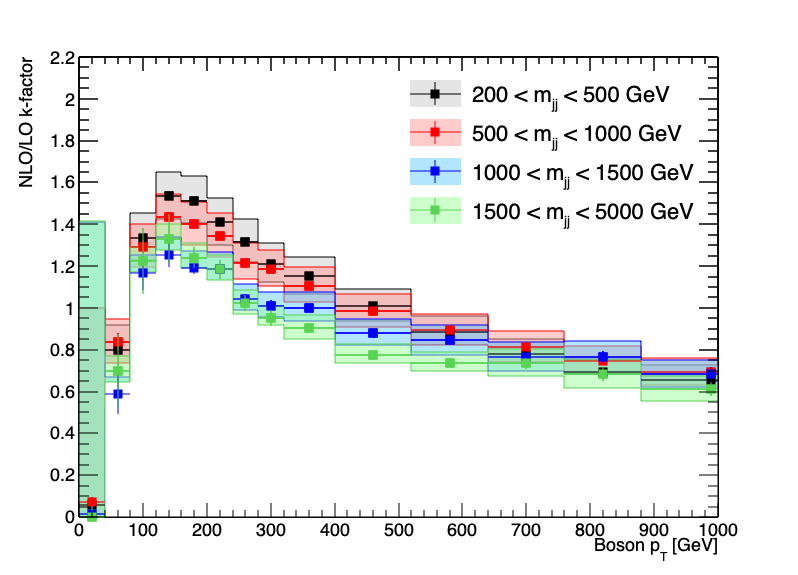
\includegraphics[width=0.49\textwidth]{Objects/kfactor_VBF_zjet_born_default.png}}
        \subfigure[W~$\rightarrow l\nu$+jets]{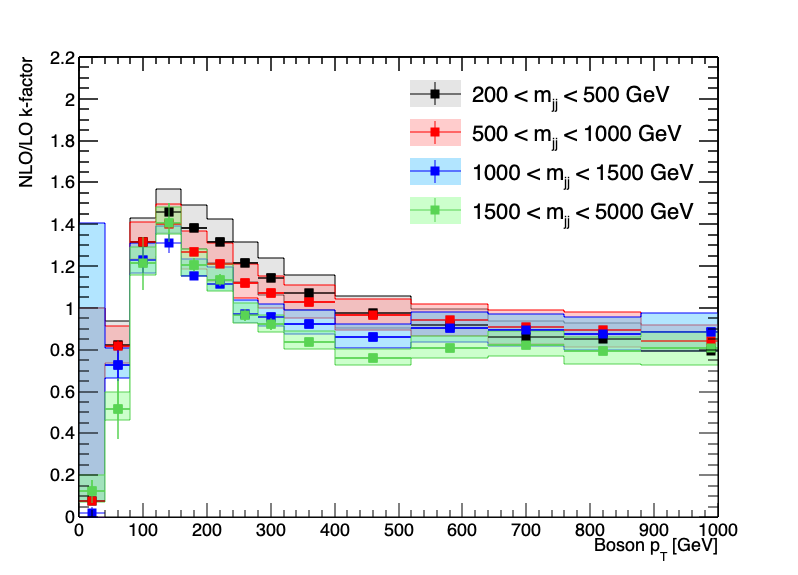
\includegraphics[width=0.49\textwidth]{Objects/kfactor_VBF_wjet_born_default.png}} \\
        \subfigure[Z~$\rightarrow\nu\nu$+jets]{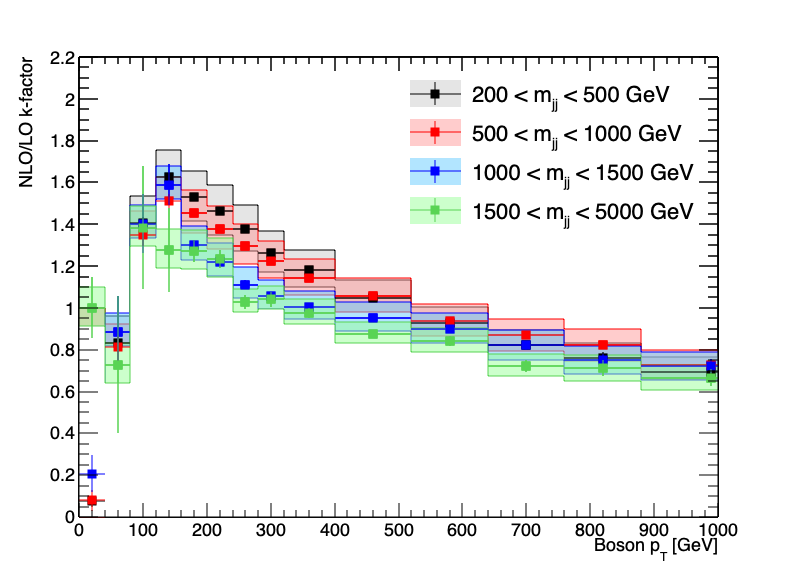
\includegraphics[width=0.49\textwidth]{Objects/kfactor_VBF_znn_born_default.png}}
        \caption{
            The LO-to-NLO theory scale factors binned in the generator level $p_T^V$ and $m_{jj}$, shown for QCD V+jets processes.
            The scale factors are derived within the generator level selection requirements equivalent to the ones used to form the analysis category defined in Section~\ref{subsec:vbfselection}. The error bars reflect the statistical uncertainty on the bin, while the bands represent the total systematic uncertainty~\cite{note:AN_19_257}.}
      \label{fig:theory_sf_qcd_nlo_2d}
    \end{center}
  \end{figure}
  
  \begin{figure}[htbp]
    \centering
       \subfigure[Z~$\rightarrow ll$+jets]{ 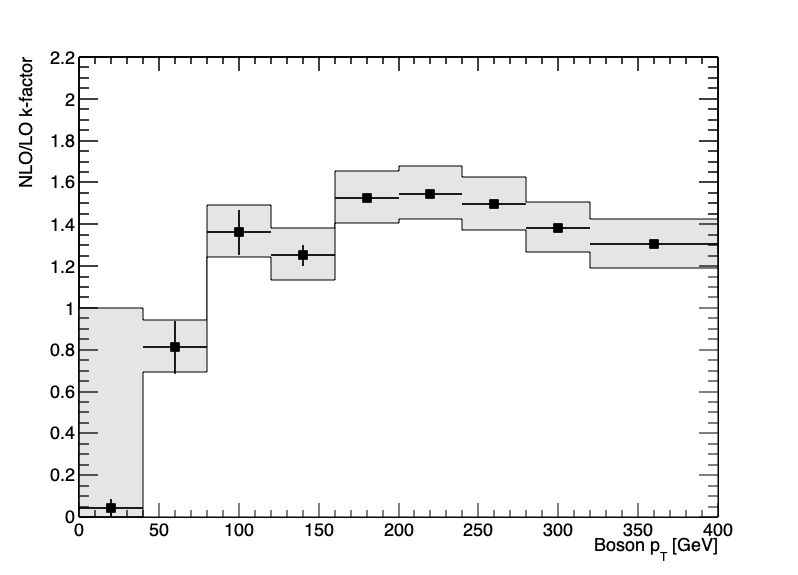
\includegraphics[width=0.49\textwidth]{Objects/kfactor_VTR_zjet_born_default.png}}
        \subfigure[W~$\rightarrow l\nu$+jets]{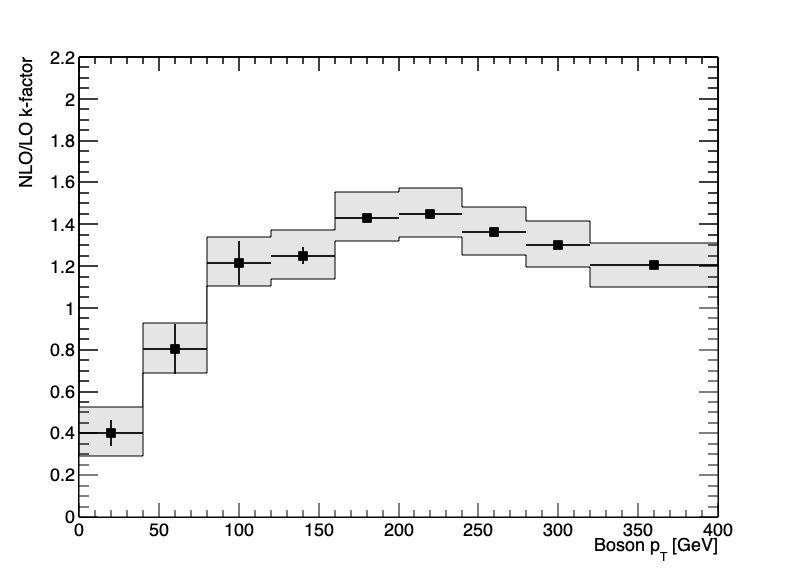
\includegraphics[width=0.49\textwidth]{Objects/kfactor_VTR_wjet_born_default.png}} \\
        \subfigure[Z~$\rightarrow\nu\nu$+jets]{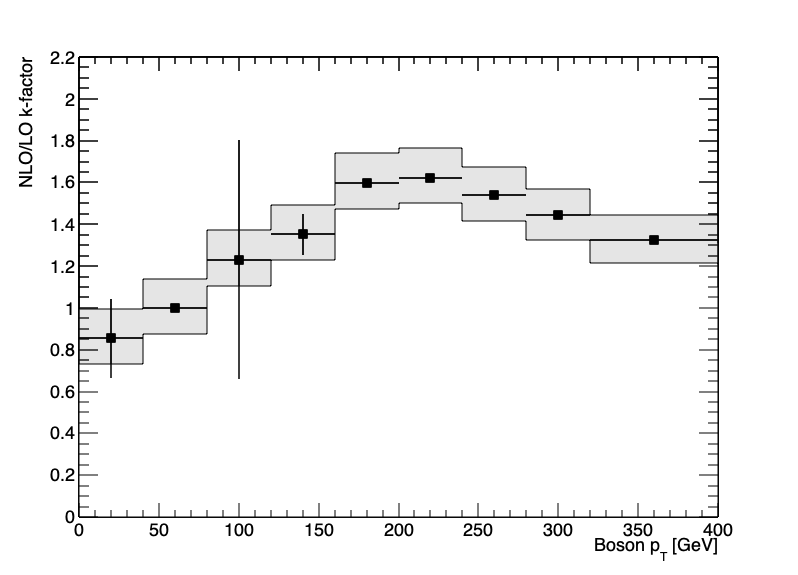
\includegraphics[width=0.49\textwidth]{Objects/kfactor_VTR_znn_born_default.png}}
    \caption{The LO-to-NLO theory scale factors binned in generator level $p_T^V$, shown for QCD V+jets processes.
            The scale factors are derived within the generator level selection requirements equivalent to the ones used to form the analysis category defined in Section~\ref{subsec:vtr_selection}. The error bars reflect the statistical uncertainty on the bin, while the bands represent the total systematic uncertainty~\cite{note:AN_19_257}.}
    \label{fig:nlo-kfactors-w_n_z-vbf-vtr}
\end{figure}

\chapter{Analysis strategy}
\label{ch:an_strategy}
\epigraph{\itshape``All men can see these tactics whereby I conquer, but what none can see is the strategy out of which victory is evolved."}{--- \textup{Sun Tzu}}

\section{Introduction}
\hspace{10pt}This chapter serves to present a detailed documentation of the analysis strategy used for the search for the invisibly decaying Higgs bosons, where the Higgs boson is produced via the Vector Boson Fusion production mechanism. The study at hand has had a long history within the CMS experiment starting all the way back from the early days of Run 1~\cite{paper:HIG_17_023}. This thesis tends to build on conclusions and methods achieved with previous efforts by improving them where possible, while also taking the advantage of the full Run 2 dataset.

\hspace{10pt} Each of the following sections is going to summarize motivations and definitions that came into fruition while forming two main categories. Special attention will be given to the analysis category based around new, production mode targeting triggers introduced in Section~\ref{sec:vbf_trgger}, which allowed for further exploration of the signal sensitive phase space. Being a large part of motivation influencing the selection requirements, performance studies of analysis related trigger algorithms are going to be presented at this stage. Finally, this chapter concludes with a discussion regarding additional data quality issues plaguing 2017 and 2018 eras of data taking and studies performed in order to mitigate their effects on the final result.

\hspace{10pt} In order to be consistent with the notation used in Chapter~\ref{ch:combination}, which combines results from all hadronic production modes of the Higgs boson, a simple naming convention is going to be used when addressing certain analyses (due to common motivations and data quality issues plaguing them). This convention is based on the two main focuses in terms of the preferred Higgs boson production mode. All studies focusing on the Higgs boson produced via the vector boson fusion will be grouped under one roof named the ``VBF analysis'', while the remaining modes of interest such as the ttH, gluon-gluon fusion (ggH) and the VH production will represent the ``non-VBF analysis''.
\section{Selection requirements}
\hspace{10pt} This section serves as summary of two main analysis categories. In order to simplify the way of addressing different categories within the VBF analysis, the following notation is going to be used in future text. All studies being built around the $E_{T,miss}$ and $H_{T,miss}$ triggers shown in Table~\ref{tab:metmht} are going to be part of the Missing Energy Trigger (MTR) category. On the other hand, the new category being formed through the usage of VBF production mode targeting triggers (listed in Table~\ref{tab:hlt_rates}) is going to be named the VBF Trigger (VTR) category. A complete set of information regarding the L1 seeds used as inputs to the HLT algorithms forming these analysis categories is given in the form of Table~\ref{a_tab:triggers}.

\hspace{10pt} The common ground for both categories is the approach to rejecting the contributions from major sources of SM background when forming the signal region (SR) through the implementation of object vetos. In order to battle the reducible contribution coming from main V+jets backgrounds a $\mu/e/\tau$ vetos are imposed. A similar approach is taken in order to contain the $\gamma$+jets processes with the a veto on photon objects being put in place. Finally, a b jet object veto requirement tends to remove the reducible background originating from top quark SM processes. The interpretation of the aforementioned vetos follows the strategy described in Section~\ref{sec:object_corr}, where it is stated that a veto weight is applied for simulation samples as opposed to a $N_{object}=0$ condition, which is being used for data. The following pages are going to introduce the main selection criteria for each of the categories.
\subsection{Missing Energy Trigger category}
\label{subsec:vbfselection}

\hspace{10pt} This category follows the strategy published with the results originating from data collected in 2016~\cite{paper:HIG_17_023}. It is represented with the requirements shown in Table~\ref{tab:selection_mtr}. With the set of object vetos already covered in the introduction, the discussion regarding the rest of the requirements can be split into two categories. Their origin can be traced to be either related to the topological properties expected from VBF jets, introduced in order to reduce a major contribution from SM processes, or they are purely motivated by the performance of HLT algorithms used for data collection.

\begin{table}[htbp]
\centering
%\small
\begin{tabular}{lcc}
    Variable                           & Selection                       & Target background \\
    \hline
    & & \\
    $\mu$ ($e$) veto               & $p_T > 10$~GeV,~$|\eta| < 2.4 (2.5)$  & $Z(ll)$~+jets,~$W(l\nu)$~+jets \\
    $\tau$ lepton veto                 & $p_T > 20$~GeV,~$|\eta| < 2.3$        & $Z(ll)$~+jets,~$W(l\nu)$~+jets  \\
    $\gamma$ veto                        & $p_T > 15$~GeV,~$|\eta| < 2.5$        & $\gamma$~+jets \\
    b jet veto                    &  $p_T > 20$~GeV,~$|\eta| < 2.4$  &  Top quark\\
        & & \\
    $E_{T,miss}$                          & ${>} 250$~GeV                          & QCD, top quark, $Z(ll)$~+jets \\
    $min\Delta\phi(j, E_{T,miss})$   &  $ {>} 0.5$ radians               & QCD \\
    $|$1$-E_{T,miss}^{Calo}/E_{T,miss}|$   &  $ {<} 0.5$               & QCD \\
        & & \\
    $p_{T,j_1}$ and $\eta_{j1}$   & ${>} 80$~GeV and $ |\eta| < 4.7$      & All \\
    $p_{T,j_2}$ and $\eta_{j2}$   & ${>} 40$~GeV and $ |\eta| < 4.7$      & All \\
    $\eta_{j1}\cdot\eta_{j2}$   & ${<}$ 0   & All \\

    $m_{jj}$                               & ${>} 200$~GeV  \\       
    $\Delta\eta_{jj}$                            & ${>} 1.0$  \\
    $\Delta\phi_{jj}$                            & ${<} 1.5$  \\
        & & \\
         \hline
\end{tabular}
\caption{Summary of the MTR selection requirements, accompanied with the target background processes affected by them~\cite{note:AN_19_257}}
\label{tab:selection_mtr}
\end{table}

\hspace{10pt} Starting with the topological information, the VBF signature is characterised with a jet pair which has a large geometrical separation and a large dijet mass. When interpreted in terms of the detector geometry (introduced in Section~\ref{sec:geometry}), this leads to conditions that jets, chosen as the two leading in $p_T$, have to be separated by a large value of $\Delta \eta$, a small $\Delta \phi$ and to have $\eta_{j1}\cdot\eta_{j2}<0$ by being in the opposite bisections of the experiment.

\hspace{10pt} Moving on from the purely topological properties, the next step is to try and determine which variables represent a good basis for additional lowering of the contribution coming from various sources of SM background. Variables such as the $min \Delta \phi (j, E_T^{miss})$\footnote{The minimal $\Delta\phi$ between the one of the four leading jets (ordered in $p_T$) and the $\vec{p}_{T, miss}$.} (where only the first four leading jets with $p_T > 30$~GeV enter the computation) allow for a better control of the QCD multijet background, Figure~\ref{fig:sr_n-1_shapes_1} shows its separation power using the N-1 selection\footnote{All of selection requirements are being applied but the one involving the variable of interest.} approach. With it showing combined background composition originating from simulation samples of SM processes being overlaid with the distribution of the signal, it can be seen that the requirement of $min \Delta \phi (j, E_{T,miss})>$~0.5 yields a significant reduction of QCD multijet backgrounds, without a large loss of signal sensitivity. Another useful requirement comes from the comparison of the offline (after the full reconstruction) and calorimeter only $E_{T,miss}$. A requirement that the relative difference is less than 50\% (when taking the offline $E_{T,miss}$ as reference) provides another way of rejecting events which contain energetic mismeasured jets originating from multijet processes. 

\hspace{10pt} As indicated at the beginning of this section, geometrical properties of the selected dijet object play a large role in the recognition of signal like events, as illustrated in Figure~\ref{fig:sr_n-1_shapes_1}. This comparison of $\Delta \eta_{jj}$ and $\Delta \phi_{jj}$ distributions between main backgrounds and signal shows a clear opening for a set of requirements which are going to further improve the selection. An optimisation procedure, taking into account the entire setup for the analysis (including the contributions from dedicated control regions), was performed~\cite{paper:HIG_17_023} in order to obtain thresholds presented in Table~\ref{tab:selection_mtr}. 

\hspace{10pt} Finally, there are requirements that are arising strictly from trigger limitations. This can be seen in the choice of the $E_{T,miss}$ threshold, where the requirement on it being larger than $250$~GeV was imposed in order to stay above the $95$~\% efficiency for the category-forming triggers, when measured in data. This efficiency gets above $99$~\% for the values of $E_{T,miss}>300$~GeV. A more detailed documentation of this measurement is given in Section~\ref{subsec:mtr_triggers}.

\hspace{10pt} Figure~\ref{fig:sr_n-1_shapes_2} shows data to simulation agreement for a selected set of main analysis variables after the application of the complete MTR selection for the 2017 era of data taking. Corresponding information regarding the SR for the 2018 era is given in Appendix~\ref{app:MTR_2018}. The scale of data to simulation disagreement illustrates the need for dedicated control regions in order to better estimate the irreducible part of the contribution originating from V+jets processes. The MTR category is constructed to represent the main analysis category, covering a large piece of the phase space of interest. In order to further improve on it, the following section is going to show a complementary category formed around a set of VBF triggers introduced in Section~\ref{sec:vbf_trgger}.

\begin{figure}[htbp]
  \centering
    \subfigure[$min\Delta\phi(j,E_T^{miss})$]{
    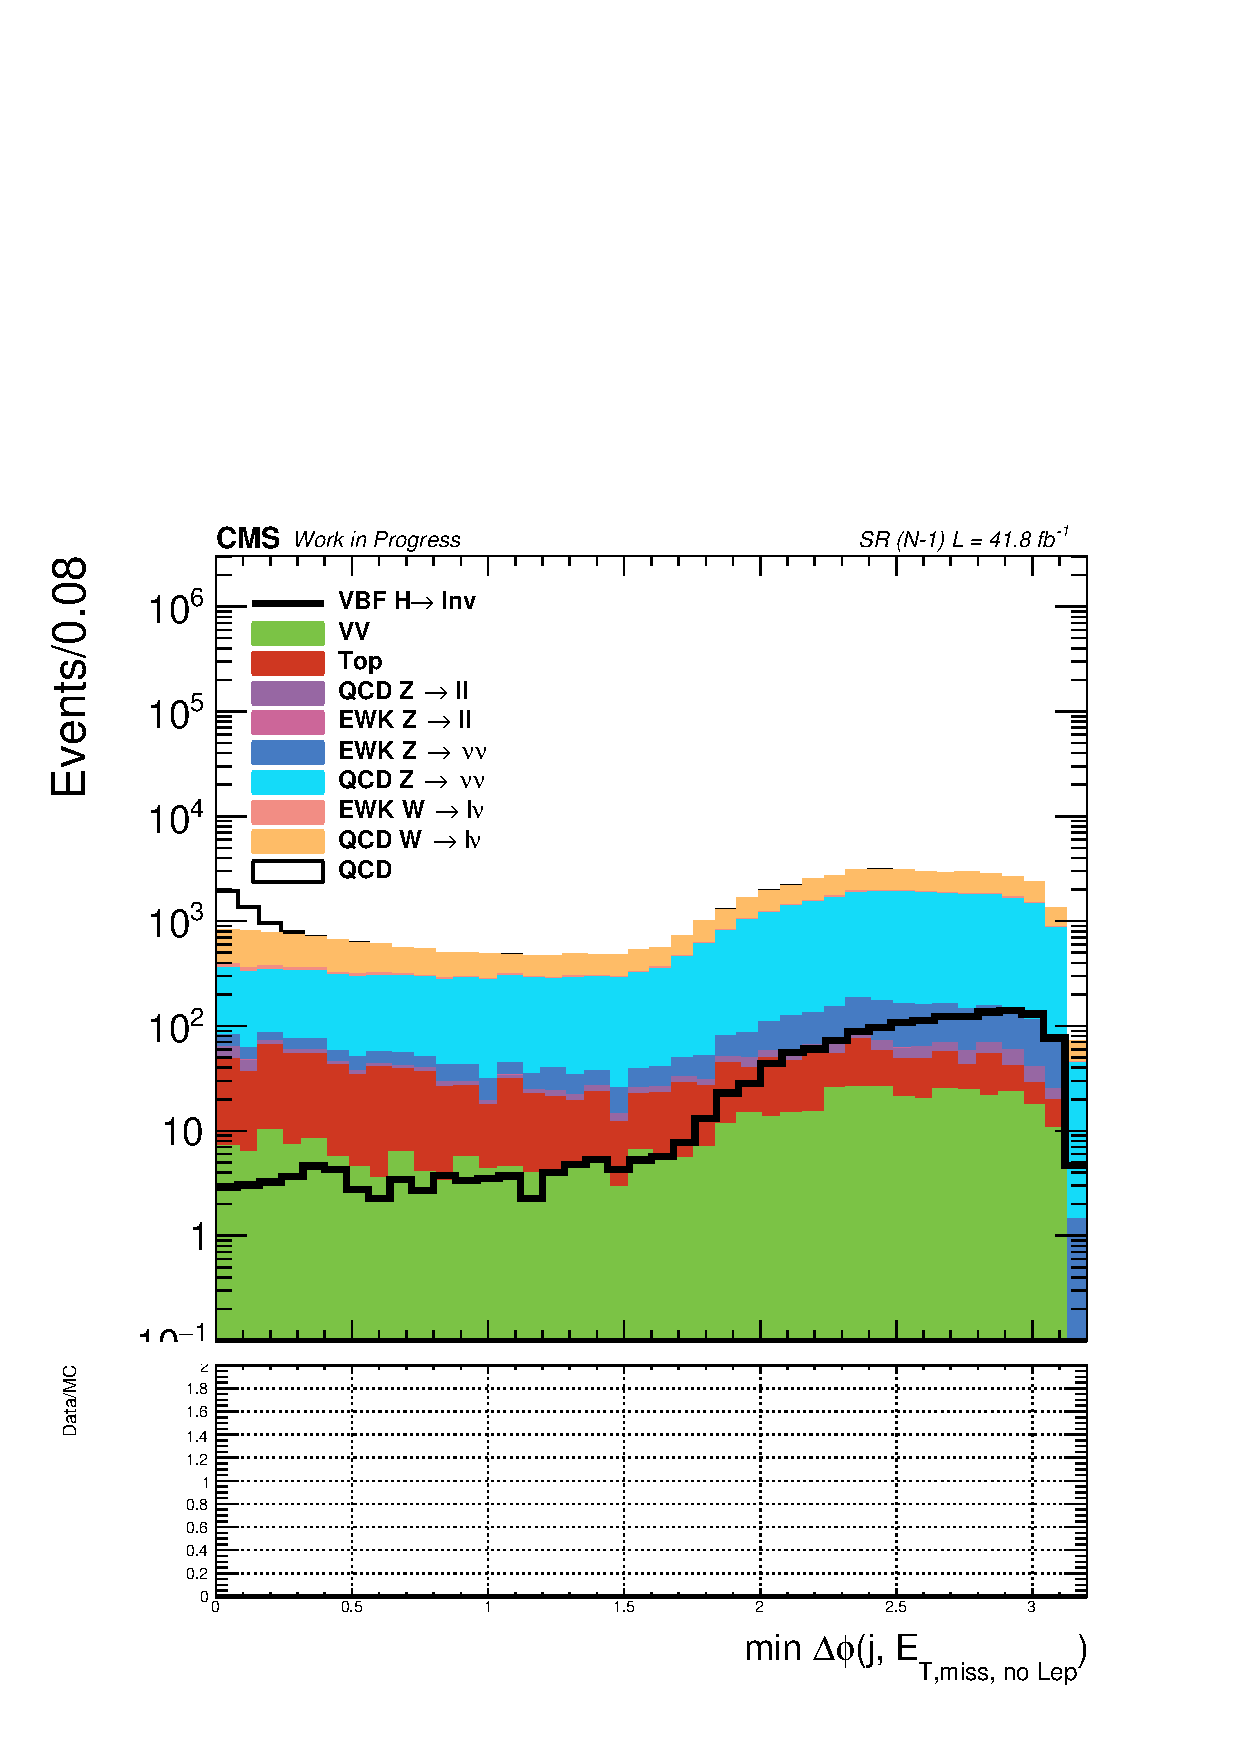
\includegraphics[width=0.49\textwidth]{Analysis_strategy/Nminus1/min_dphi_nminus1_log.pdf}
    }\\
    \subfigure[$\Delta \eta_{jj}$]{
    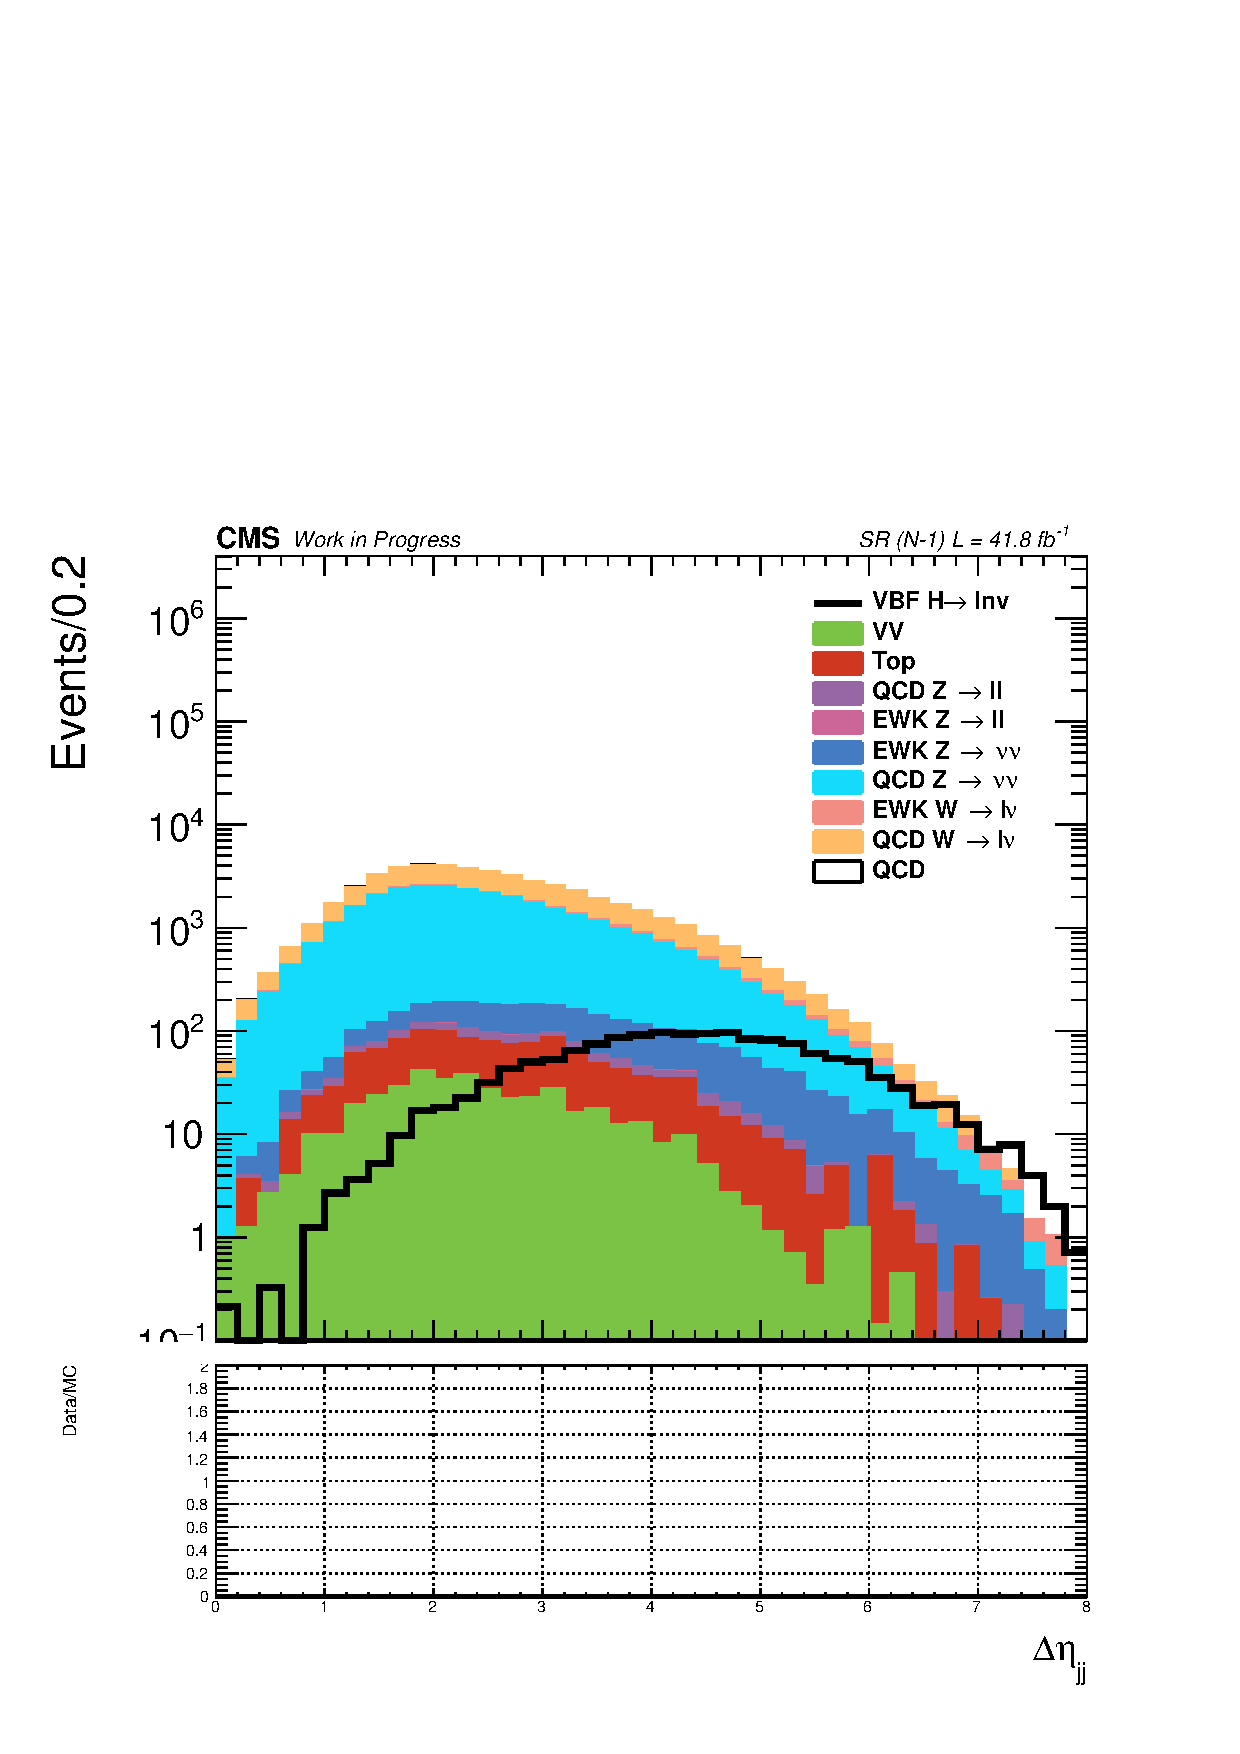
\includegraphics[width=0.49\textwidth]{Analysis_strategy/Nminus1/leading_dEtajj_nminus1_log.pdf}
    }
    \subfigure[$\Delta \phi_{jj}$]{
    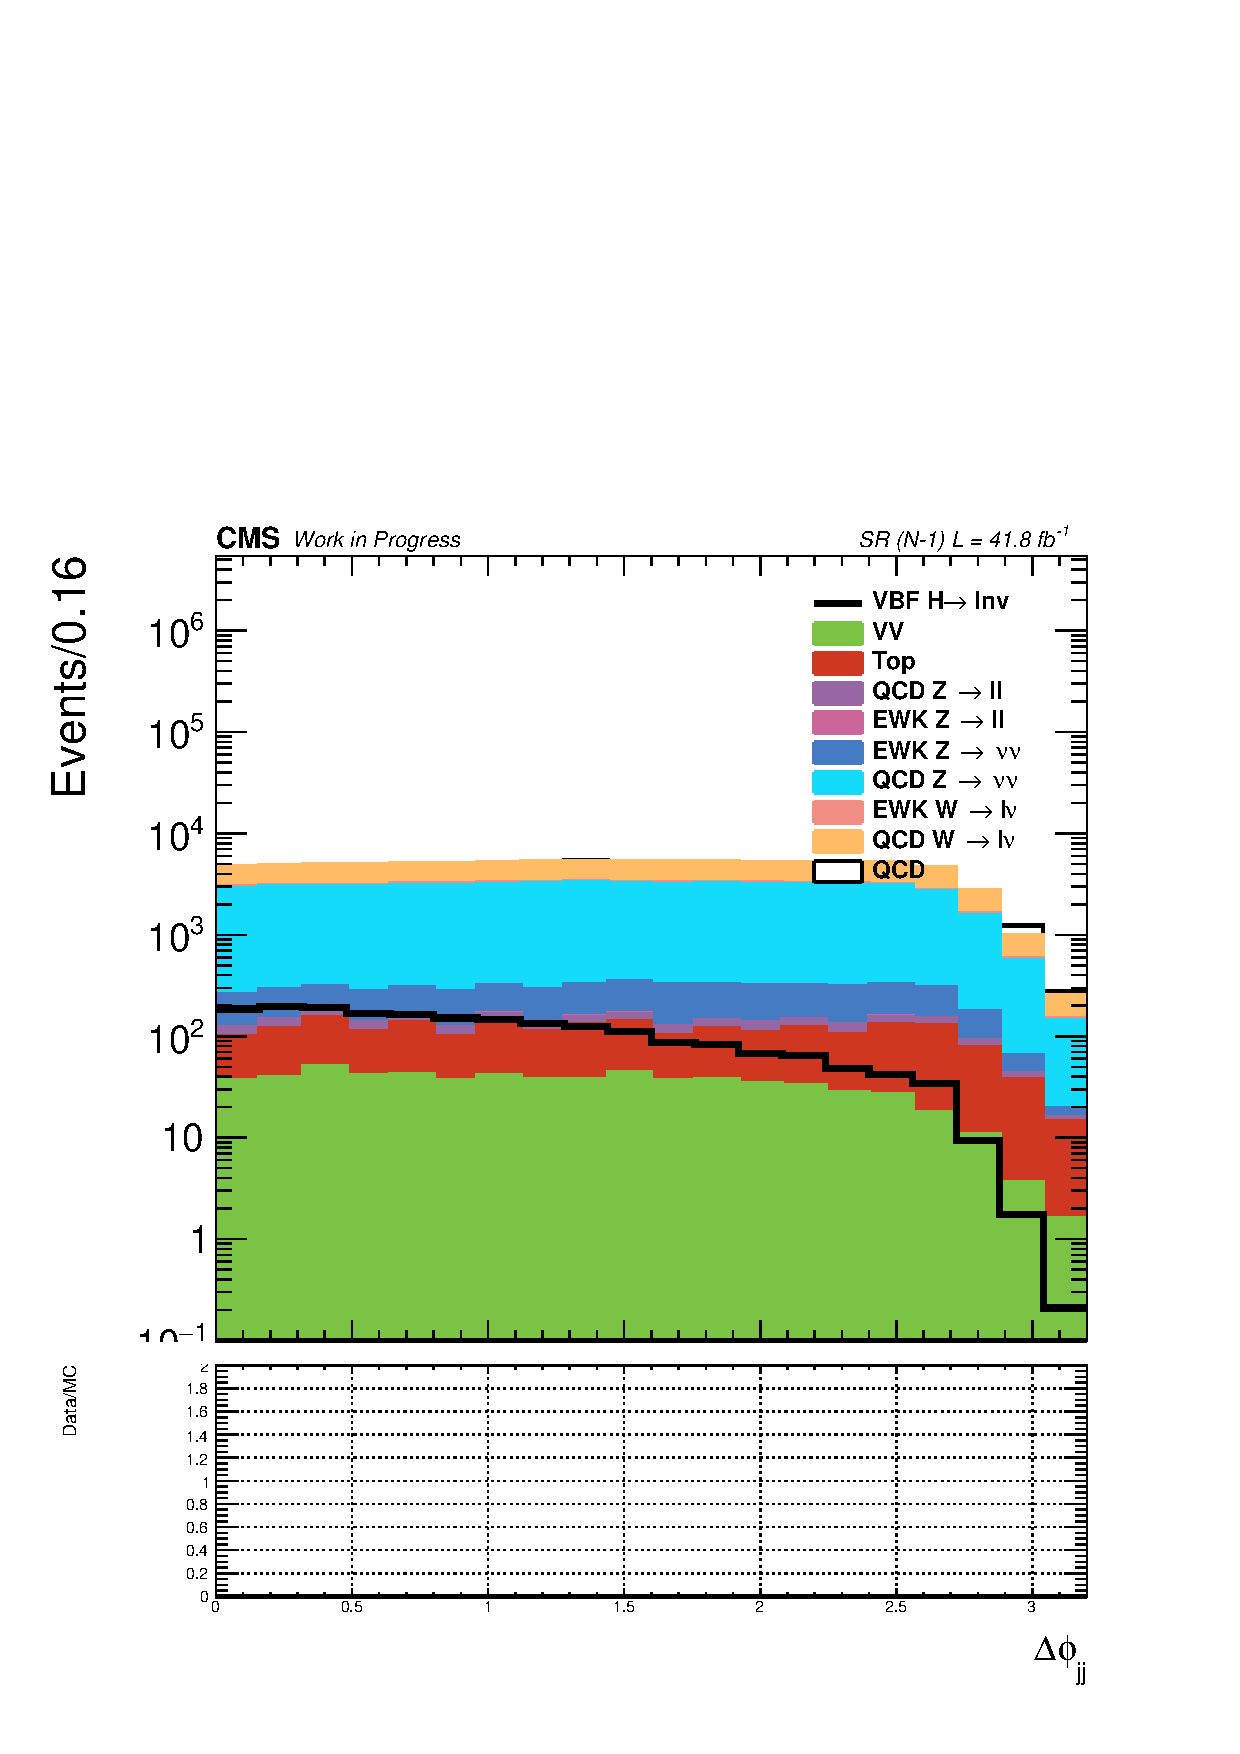
\includegraphics[width=0.49\textwidth]{Analysis_strategy/Nminus1/leading_dPhijj_nminus1_log.pdf}
    }
    
  \caption{Distributions of $min\Delta\phi(j,E_{T,miss})$, $\Delta \eta_{jj}$ and $\Delta \phi_{jj}$ variables in the SR, for the MTR category after the N-1 selection, representing the 2017 era.}
  \label{fig:sr_n-1_shapes_1}
\end{figure}


\begin{figure}[htbp]
  \centering
      \subfigure[$E_{T,miss}$]{
    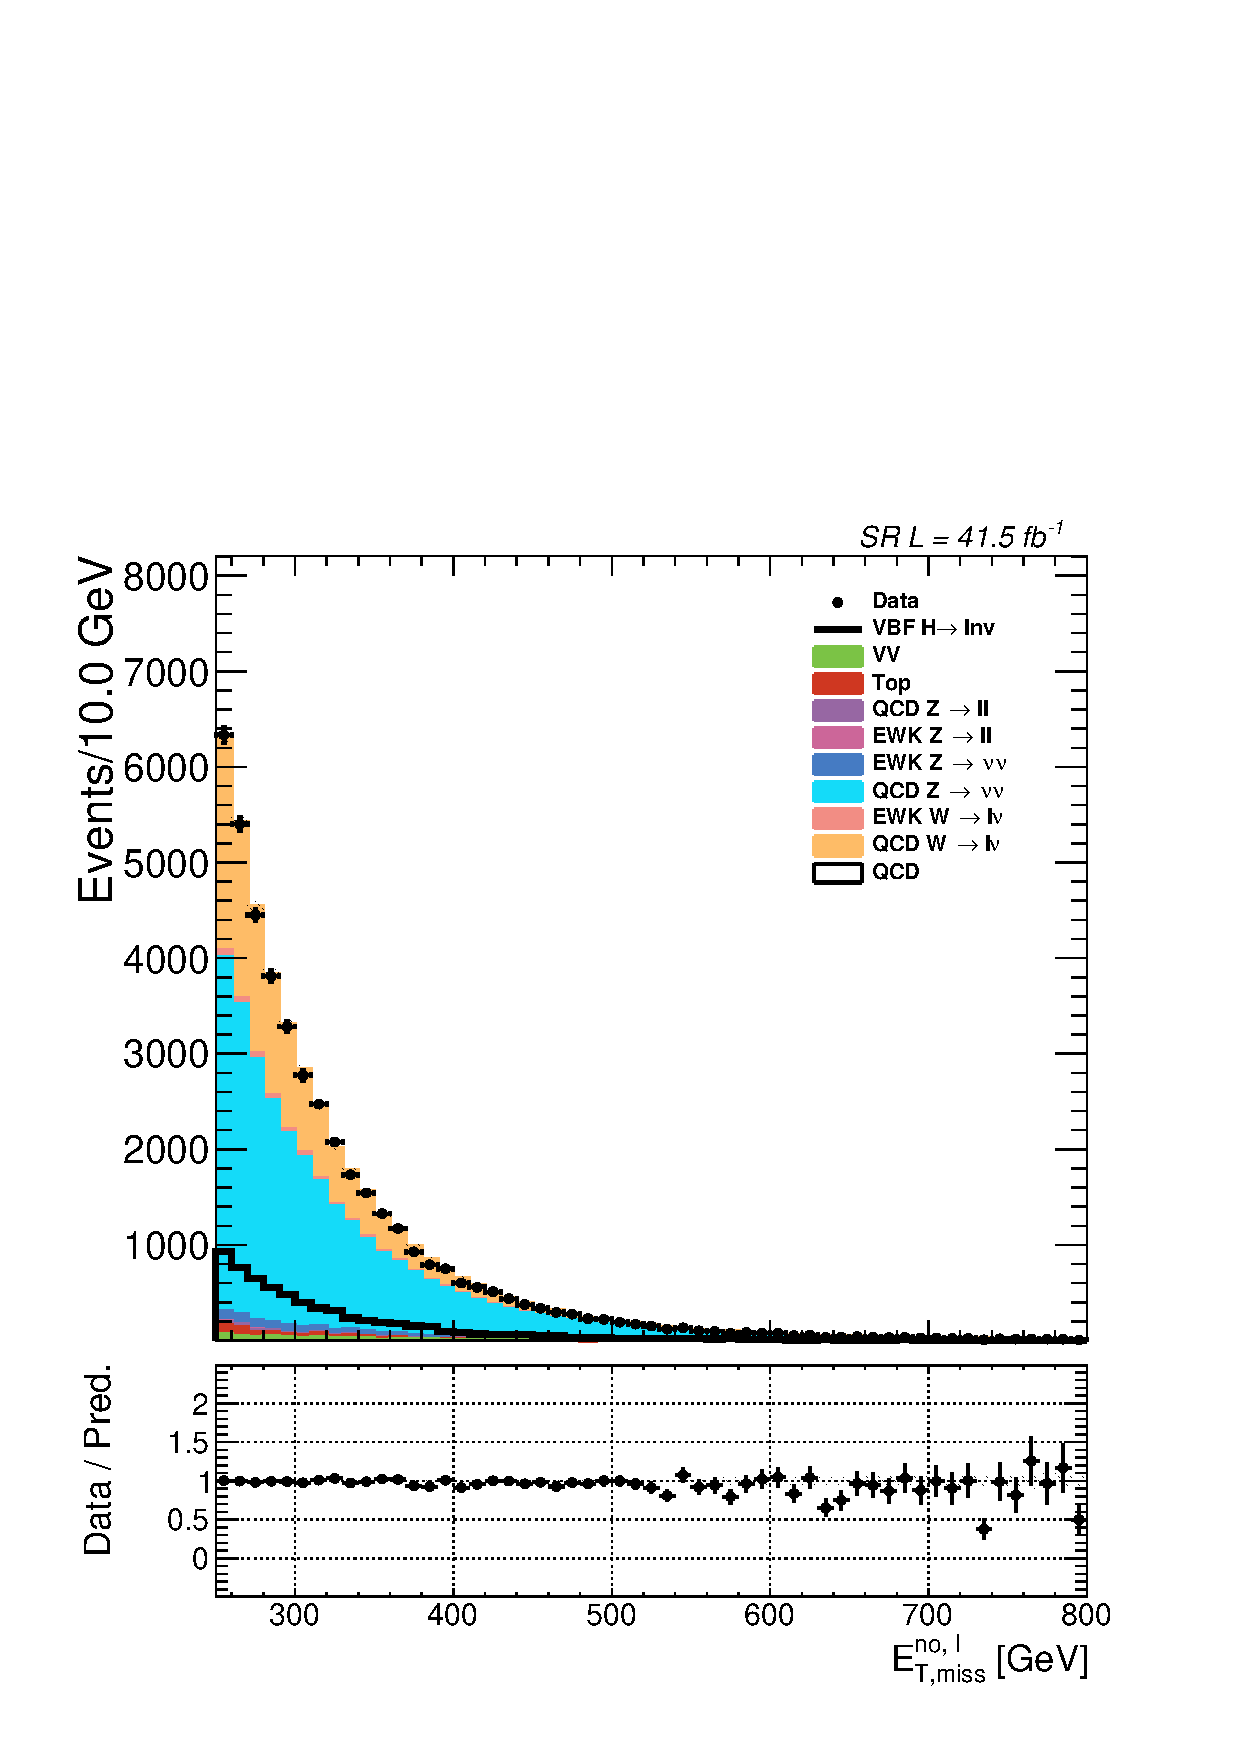
\includegraphics[width=0.49\textwidth]{Analysis_strategy/MTR_2017_SR/MetNoMu.pdf}
    }
    \subfigure[$M_{jj}$]{
    \includegraphics[width=0.49\textwidth]{Analysis_strategy/MTR_2017_SR/leadingJet_mjj.pdf}
    }\\
    \subfigure[$p_{T,j1}$]{
    \includegraphics[width=0.49\textwidth]{Analysis_strategy/MTR_2017_SR/Leading_jet_pt.pdf}
    }
    \subfigure[$p_{T,j2}$]{
    \includegraphics[width=0.49\textwidth]{Analysis_strategy/MTR_2017_SR/Subleading_jet_pt.pdf}
    }
  \caption{Distributions of $E_{T,miss}$, $M_{jj}$, $p_{T,j1}$ and $p_{T,j2}$ variables in the SR after the full MTR selection, representing the 2017 era.}
  \label{fig:sr_n-1_shapes_2}
\end{figure}







\subsection{VBF Trigger category}
\label{subsec:vtr_selection}
\hspace{10pt} Continuing the narrative started in Section~\ref{sec:vbf_trgger}, the main focus of this section is going to be the creation of a new analysis category designed to select the phase space of interest that was overlooked by the MTR category. Following the, previously discussed, blueprint for the MTR category, there is an opening to form a category that will be orthogonal to it. One way to look for its basis is to start from the comparison of performances of both trigger groups and picking an $E_{T,miss}$ range which is outside the MTR threshold, in which VBF triggers perform better than the MTR forming ones. 

\hspace{10pt} As it will be explained in Section~\ref{sec:vbf_trigger_performance}, this study results in a category formed within the $[160,250)~$GeV range of the $E_{T, miss}$ variable. In order to follow the logic deployed at the trigger level, the choice of jets at the analysis level is again based on the dijet pair which yields the largest invariant mass in the event. In retrospect, this choice follows the equivalent procedure to the one presented in Section~\ref{sec:vbf_implementation}. The jets entering the computation are required to have $p_T>$~40~GeV in order to mimic the trigger logic, while the slightly larger threshold is used to account for subtle differences between the HLT and offline jets. Upon constructing the dijet object and optimising the selection based on the trigger performance, thresholds on the values of the dijet mass and transverse momentum of the two jets were set. These selection requirements are then used to form the VTR category and are summarised in Table~\ref{tab:selection_vtr}.


\begin{table}[htbp]
\centering
%\small
\begin{tabular}{lcc}
    Variable                           & Selection                       & Target background \\
    \hline
     & & \\
    $\mu$ ($e$) veto               & $p_T > 10$~GeV,~$|\eta| < 2.4 (2.5)$  & $Z(ll)$~+jets,~$W(l\nu)$~+jets \\
    $\tau$ lepton veto                 & $p_T > 20$~GeV,~$|\eta| < 2.3$        & $Z(ll)$~+jets,~$W(l\nu)$~+jets  \\
    $\gamma$ veto                        & $p_T > 15$~GeV,~$|\eta| < 2.5$        & $\gamma$~+jets \\
    B jet veto                    &  $p_T > 20$~GeV,~$|\eta| < 2.4$  &  Top quark\\
        & & \\
    $E_{T,miss}$                          & $[160,250)$~GeV                          & QCD, top quark, $Z(ll)$~+jets \\
    $min\Delta\phi(j, E_{T,miss})$   &  $ {>} 1.8$ radians               & QCD \\
    $min\Delta\phi(j, E_{T,miss})$   &  $ {>} 0.5$ radians               & QCD \\
        & & \\
    Largest $m_{jj}$                               & ${>}$ 900~GeV  \\       
    $p_{T,j_1}$ and $\eta_{j1}$   & ${>} 140$~GeV and $ |\eta| < 4.7$      & All \\
    $p_{T,j_2}$ and $\eta_{j2}$   & ${>} 70$~GeV and $ |\eta| < 4.7$      & All \\
    $\eta_{j1}\cdot\eta_{j2}$   & ${<}$ 0   & All \\
    $\Delta\eta_{jj}$                            & ${>} 1.0$  \\
    $\Delta\phi_{jj}$                            & ${<} 1.5$  \\
      & & \\
         \hline
\end{tabular}
\caption{Summary of the VTR selection requirements, accompanied with the target background processes affected by them~\cite{note:AN_19_257}.}
\label{tab:selection_vtr}
\end{table}

\hspace{10pt} This approach ensures the "out of the box" orthogonality between two analysis categories. The high thresholds for jet $p_T$ values and the large dijet mass requirement reduce the difference between two choices of VBF jets between categories. The requirements on the $\Delta\eta_{jj}$ and $\Delta\phi_{jj}$ are directly constrained by this, allowing for the usage of the same, previously optimised, requirements from the MTR category.

\hspace{10pt} On the other hand, as this approach follows the logic given by the trigger, it is expected to bring a certain amount of QCD multijet events as well. As seen in the previous section, a good handle for dealing with these processes is given in the form of the $min\Delta\phi(j, E_{T,miss})$ variable. Figure~\ref{fig:VTR_mindphi} shows the distribution of this variable in the VTR SR after the application of a looser ($>0.5$) requirement. It can be seen that values bellow 1.8 are largely background dominated, with the QCD multijet processes leading the way, while being populated with a low yield of signal events, thus motivating a requirement which would remove this region without risking a significant loss in signal acceptance. 

\begin{figure}[htbp]
  \centering
    \subfigure{
    \includegraphics[width=0.49\textwidth]{Analysis_strategy/Nminus1/VTR/MetNoLep_CleanJet_mindPhi_FAST_log.pdf}
    }
  \caption{Distribution of the \mindphi~variable in the SR after the VTR-like selection requirements.}
  \label{fig:VTR_mindphi}
\end{figure}
Figure~\ref{fig:VTR_SR_2017} shows the data to simulation comparisons for a few selected variables after the full VTR selection. A set of dedicated control regions will be created for the VTR category, analogous to the MTR approach, in order to improve the overall data to simulation agreement. In order to efficiently illustrate the discussion given in these two sections, only the 2017 era of data taking was presented for both MTR and VTR categories. Additional set of distributions for VTR category representing the 2018 era is given in Appendix~\ref{app:MTR_2018} alongside their MTR counterparts. 


%first step will be to see how this orthogonality can be achieved on the selection level. Following the trigger turnons given in Figures [TBD] and the definition of the MTR category (introduced in the prvious paragraph), it can be seen that a $E_T^{miss}$ range of $[160,250)~$GeV represents a good requirement that would clearly establish the separation between two categories. Figures [TBD] and [TBD] showcase the Signal Region for the VTR category taking into account two selection options showcased in Section~\ref{sec:triggers}. Based on the conclusion of that section (and also taking into account that both options give similar event yields), option B, where the HLT selection logic is followed, will be used to define the VTR category. Additionally a higher requirement on $min\Delta\phi(jet,~E_T^{miss,~no~lep})>1.8$ has been added to reduce the contribution from multijet processes. 




\begin{figure}[htbp]
  \centering
    \subfigure[$\Delta \eta_{jj}$]{
    \includegraphics[width=0.49\textwidth]{Analysis_strategy/VTR_2017_SR/lMjj_leading_dEtajj.pdf}
    }
    \subfigure[$\Delta \phi_{jj}$]{
    \includegraphics[width=0.49\textwidth]{Analysis_strategy/VTR_2017_SR/lMjj_leading_dPhijj.pdf}
    }\\
    \subfigure[$m_{jj}$]{
    \includegraphics[width=0.49\textwidth]{Analysis_strategy/VTR_2017_SR/lMjj.pdf}
    }
    \subfigure[$E_{T,miss}$]{
    \includegraphics[width=0.49\textwidth]{Analysis_strategy/VTR_2017_SR/MetNoMu.pdf}
    }
  \caption{Distributions of $\Delta \eta_{jj}$, $\Delta \phi_{jj}$, $m_{jj}$ and $E_{T,miss}$ variables int the signal region after the full VTR selection, representing the 2017 era.}
  \label{fig:VTR_SR_2017}
\end{figure}


\section{Trigger Performance}

\hspace{10pt} The following sections focus on the performance of the HLT algorithms used in this analysis. These paths can be split into two groups based on their usage: the signal/muon region and the electron region forming triggers. The added benefit of the signal triggers (listed in Tables~\ref{tab:hlt_rates} and~\ref{tab:metmht}) comes from the fact that they are built by adding conditions on $E_{T, miss}^{~no, \mu}$ (as seen in the diagram presented in Figure~\ref{fig:VBF_HLT}). The $\vec{p}_{T, miss}^{~no, \mu}$ vector, whose intensity is represented by $E_{T, miss}^{~no, \mu}$, is defined by adding the transverse momentum of muon objects back into the $\vec{p}_{T, miss}$ computation. This can be expressed as:
\begin{equation}
  \vec{p}_{T, miss}^{~no, \mu} = \vec{p}_{T, miss} + \sum_i \vec{p}_{T,\mu_i},
\end{equation}
where the sum goes over all muon objects. Such definition of the missing energy is equivalent to the standard $E_{T, miss}$ for the SR, due to the usage of a muon veto. This re-definition extends the usability of aforementioned trigger algorithms, which can now be used to select events entering muon regions (more details about these specialised regions are given in Section~\ref{sec:control_regions}). For the regions containing electron objects, a combination of electron and photon triggers is used. The addition of photon triggers was performed in order to achieve better statistics in these regions (which will benefit the double electron region, due to its tight requirements). The complete list of HLT paths used in this analysis (and the corresponding L1 seeds used as input) is given in Table~\ref{a_tab:triggers}.

\subsection{Performance of $E_T^{miss}$ and $H_T^{miss}$ based triggers}
\label{subsec:mtr_triggers}
\hspace{10pt} Following the ordering used in the previous section, the first topic of discussion is going to be the performance of triggers used to form the MTR category. Listed in Table~\ref{tab:metmht}, they are represented by a set of selection requirements on $E_{T,miss}^{~no,\mu}$ and $H_{T,miss}^{no,~mu}$ variables at the HLT stage. This section is going to summarize the study of their performance during the 2017 and 2018 era of data collection. It is going to be based around the analysis selection requirements for the MTR category (as shown in Table~\ref{tab:selection_mtr}), presenting the motivation behind the $E_{T,miss}$ threshold (which is set with respect to the overall performance). More details about the choice of the selection itself can be found in Section~\ref{subsec:vbfselection}.

\begin{table}[htbp]
\centering
%\small
\begin{tabular}{l|c}
\hline\hline
Era & Trigger name                                               \\ \hline
\multirow{4}{*}{2017 \& 2018} &\\
                      &\texttt{HLT\_PFMETNoMu120\_PFMHTNoMu120\_IDTight\_PFHT60}\\
                        &\texttt{HLT\_PFMETNoMu120\_PFMHTNoMu120\_IDTight}\\ 
                        &\\\hline
\hline\hline
\end{tabular}
\caption{List of $E_{T,miss}$ and $H_{T,miss}$  triggers used in the analysis. Conventional names are used to describe the HLT level requirements imposed on the variables, with them being: $E_{T,miss}^{~no,\mu}>$ 120~GeV and $H_{T,miss}^{~no,\mu}>$ 120~GeV (with the addition of the $H_T>$~60~GeV requirement for the backup path).  \label{tab:metmht}}
\end{table}
\hspace{10pt} During the 2017 era of data taking, a special, control, version of main $E_{T,miss}$ path had to be introduced, as the main one was prescaled due to problems which led to the drastic increase of its rate. The origin of this problem is connected to the same issues plaguing the L1 VBF seed as explained in Section~\ref{sec:vbf_trgger}. This has resulted in the inclusion of the additional $H_T>$60~GeV requirement at the trigger level. This issue was quickly mitigated in 2017 by applying slightly higher thresholds on the input L1 seeds, thus reducing the amount of rate brought by the trigger. This backup path was kept for the entirety of 2018 era, but with certain modifications applied to its input. As it was noticed that it brought an efficient reduction in rate when used as a backup, it was redeployed with lower requirements applied to the input L1 seeds, allowing for it to be used alongside the main path in the analysis.

\hspace{10pt} The general approach when measuring efficiencies for both eras is to form dedicated regions in which the actuall measurement will be performed. For this study this is done by using a slightly modified definition of a single muon control region. As described in Section~\ref{sec:single_muon}, this modified the muon veto condition by asking for the existence of exactly one muon object in the event which passes the tight conditions. For the measurement itself, a control HLT path is being used (\texttt{HLT\_IsoMu27}), which represents a single muon trigger looking for muon objects with $p_T>$27~GeV which pass the isolation requirement at the HLT level. In order to ensure that the study is performed in a region of high control trigger efficiency (on the trigger "plateau"), a requirement $p_{T,\mu}>30$~GeV is imposed on the selected tight muon. The efficiency measurement is presented in terms of $E_{T,miss}^{~no,\mu}$ bins and defined as:

\begin{equation}
\text{Efficiency} = \frac{(\text{Passing analysis selection requirements})~and~(\text{HLT triggered})}{\text{Passing analysis selection requirements}},
\end{equation}

The efficiency of the logical OR of the two HLT paths is measured both in data and simulation, while the resulting difference is being used as a scale factor which is applied, in main analysis, to simulation samples on an event by event basis (as described in Section~\ref{sec:object_corr}). Inputs for these measurements are formed from the muon enriched dataset (Single Muon PD) and the QCD W+jets simulaton samples, representing the dominant SM process in this region. Figure~\ref{fig:metmht_effs} presents the resulting efficiencies, with the corresponding scale factors, for both 2017 and 2018 eras.

\begin{figure}[htbp]
  \centering
    \subfigure[2017]{
    \includegraphics[width=0.45\textwidth]{Analysis_strategy/METMHT_eff/MetNoMuMETMHT_2017.pdf}
    }
    \subfigure[2018]{
    \includegraphics[width=0.45\textwidth]{Analysis_strategy/METMHT_eff/MetNoMuMETMHT_2018.pdf}
    }
  \caption{Trigger efficiencies for the MTR forming algorithms presented in $E_{T.miss}^{no,\mu}$ bins for both eras. Separate efficiencies were measured for data and simulation with the resulting scale factor also being shown.}
  \label{fig:metmht_effs}
\end{figure}


\hspace{10pt} An additional set of efficiencies was produced by separating jets into three categories by looking at the geometrical properties of the two leading jets. This has resulted into three categories: two central jets (CC), one central, one forward jet (CF) and two forward jets (FF). This study was prompted as safety check in order to confirm that a previously reported dip in $m_{jj}$ efficiency during the 2016 era~\cite{note:AN_16_418} has disappeared after mitigation. The origin of this efficiency loss was the exclusion of the HF region from the energy sums at the L1T level. Summary of this study is that the lack of efficiency issues plaguing the previous era has been correctly removed through the addition of the HF contribution implemented for the 2017 and 2018 eras. Figure~\ref{fig:metmht_test} summarises these results by presenting the efficiencies in both the $E_{T,miss}^{~no,\mu}$ and $m_{jj}$ bins. The added $E_{T,miss}^{~no,\mu}$ option was included in order to have a confirmation that no significant deviations appear between two higher statistics regions (CC and CF).


\begin{figure}[htbp]
  \centering
    \subfigure[$E_T^{miss}$ - 2017 (data)]{
    \includegraphics[width=0.45\textwidth]{Analysis_strategy/METMHT_eff/MetNoMuMETMHT_2017data_case_study.pdf}
    }
    \subfigure[$E_T^{miss}$ - 2017 (simulation)]{
    \includegraphics[width=0.45\textwidth]{Analysis_strategy/METMHT_eff/MetNoMuMETMHT_2017mc_case_study.pdf}
    }\\
    \subfigure[$E_T^{miss}$ -  2018 (data)]{
    \includegraphics[width=0.45\textwidth]{Analysis_strategy/METMHT_eff/MetNoMuMETMHT_2018data_case_study.pdf}
    }
    \subfigure[$E_T^{miss}$ -  2018 (simulation)]{
    \includegraphics[width=0.45\textwidth]{Analysis_strategy/METMHT_eff/MetNoMuMETMHT_2018mc_case_study.pdf}
    }
  \caption{Trigger efficiencies for the MTR forming algorithms presented in $E_{T.miss}^{no,\mu}$ bins for both eras (computed for data and simulation). Separation into three different jet $\eta$ regions (CC, CF and FF) is performed. The resulting comparison between the CC and CF is also presented with the ratio plot. }
  \label{fig:metmht_test}
\end{figure}


\begin{figure}[htbp]
  \centering
    \subfigure[$m_{jj}$ - 2017 (data)]{
    \includegraphics[width=0.45\textwidth]{Analysis_strategy/METMHT_eff/MetNoMuMETMHT_2017data_case_study.pdf}
    }
    \subfigure[$m_{jj}$ - 2017 (simulation)]{
    \includegraphics[width=0.45\textwidth]{Analysis_strategy/METMHT_eff/MetNoMuMETMHT_2017mc_case_study.pdf}
    }\\
    \subfigure[$m_{jj}$ - 2018 (data)]{
    \includegraphics[width=0.45\textwidth]{Analysis_strategy/METMHT_eff/MetNoMuMETMHT_2018data_case_study.pdf}
    }
    \subfigure[$m_{jj}$ - 2018 (simulation)]{
    \includegraphics[width=0.45\textwidth]{Analysis_strategy/METMHT_eff/MetNoMuMETMHT_2018mc_case_study.pdf}
    }
  \caption{Trigger efficiencies for the MTR forming algorithms presented in $m_{jj}$ bins for both eras (computed for data and simulation). Separation into three different jet $\eta$ regions (CC, CF and FF) is performed. The resulting comparison between the CC and CF is also presented with the ratio plot.}
  \label{fig:metmht_test}
\end{figure}

%\hspace{10pt} In order to ensure that the variations between regions have been accounted for, a comparison of trigger efficiencies for the single and double muon regions is performed. The double muon region is formed in mostly the same way as the single muon region, with the difference being the request that there exist exactly two muons (at least one of which needs to pass the tight requirements) in the event. Conclusion on regarding this study.


%%%%%%%%%%%%%% END OF METMHT PART %%%%%%%%%%%%%%%%%%%%%%%%%%%%%%%%




\subsection{Performance of VBF triggers}
\label{sec:vbf_trigger_performance}

\hspace{10pt} Similarly to previously described efficiency study regarding the MTR forming triggers, the first step when approaching the VBF triggers is the formation of the single muon region. From this point, the general approach takes a slightly different turn. As the MTR category relied on already proven, optimised selection, the VBF triggers brought a new part of the phase space that is yet to be explored. Staring from the information about the building blocks of VBF paths (discussed in Section~\ref{sec:vbf_trgger}), the next step was the optimisation the of the selection requirements for three main variables: $m_{jj}$, $p_{T,j1}$ and $p_{T,j2}$. In order to follow the trigger logic, the selection of the dijet pair is going be based around the largest $m_{jj}$ logic.

\hspace{10pt} Figure~\ref{fig:vbf_trig_mjj_opt} shows the resulting efficiency of the logical OR of both VBF triggers presented in terms of $m_{jj}$ bins, where the thresholds for the other two main variables are being kept high enough to ensure that an unbiased decision can be made. The resulting requirement of $m_{jj}>$~900~GeV is motivated by the desire to stay above the $95$~\% trigger efficiency in data. Figure~\ref{fig:vbf_trig_pt_opt} presents results of equivalent optimisation studies performed for the purposes of tailoring selection requirements for the jet $p_T$ variables.

\begin{figure}[htbp]
  \centering
    \subfigure{
    \includegraphics[width=0.45\textwidth]{Analysis_strategy/VBF_eff/2017/lMjjVBF_1.pdf}
    }
\caption{Trigger efficiency of the logical OR of both VBF triggers (performed in data), presented in $m_{jj}$ bins used to motivate a selection requirement for this variable.}
\label{fig:vbf_trig_mjj_opt}
\end{figure}

\begin{figure}[htbp]
  \centering

    \subfigure[$p_{T,j1}$ efficiency]{
    \includegraphics[width=0.45\textwidth]{Analysis_strategy/VBF_eff/2017/lMjj_jet1_ptVBF_1.pdf}
    }
    \subfigure[$p_{T,j2}$ efficiency]{
    \includegraphics[width=0.45\textwidth]{Analysis_strategy/VBF_eff/2017/lMjj_jet2_ptVBF_1.pdf}
    }
  \caption{Trigger efficiency of the logical OR of both VBF triggers (performed in data), presented in $p_T$ bins for the leading (left) and subleading (right) jet, used to motivate selection requirements for these variable.}
  \label{fig:vbf_trig_pt_opt}
\end{figure}

\hspace{10pt} Following the high thresholds on jet properties, the difference between selecting the two leading $p_T$ jets and the ones forming the largest $m_{jj}$ is small enough that it brings the option of using the rest of the already optimised MTR requirements into the VTR selection. At this stage, these requirements form almost the final VTR category, differing only with the $min\Delta\phi(j, E_{T,miss})>$0.5 requirement. Figure~\ref{fig:vbf_proto_trig_eff} shows the data to simulation comparison of the performance of VBF triggers for both eras (for the current, proto-VTR, selection requirements).

\begin{figure}[htbp]
  \centering
    \subfigure[$E_{T,miss}$ - 2017]{
    \includegraphics[width=0.45\textwidth]{Analysis_strategy/VBF_eff/VBF_trig_2017_proto.png}
    }
    \subfigure[$E_{T,miss}$ - 2018]{
    \includegraphics[width=0.45\textwidth]{Analysis_strategy/VBF_eff/VBF_trig_2018_proto.png}
    }
  \caption{Trigger efficiency of the logical OR of both VBF triggers, presented in $E_{T,miss}$ measured using the proto-VTR selection requirements.}
  \label{fig:vbf_proto_trig_eff}
\end{figure}

\hspace{10pt} The next step is the decision on the exact $E_{T,miss}$ range used to define the VTR category. In order to have a better overview, a comparison of performances for both sets of triggers needed to be compared. Figure~\ref{fig:vbf_metmht_comp} presents the comparison between two trigger groups. Better performance of VBF triggers in the lower $E_{T,miss}^{~no, \mu}$ range has motivated the choice of the range for VTR to be [160, 250)~GeV. The overlaying shape of the VBF H$\rightarrow$inv simulation sample is placed to illustrate the potential signal gain achieved by this choice.

\hspace{10pt} Upon forming the preliminary VTR selection and observing the background composition given with Figure~\ref{fig:VTR_mindphi}, a tighter selection requirement was imposed on the $min\Delta\phi(j, E_{T,miss})$ variable in order to battle the contribution originating from QCD multijet processes. Data to simulation efficiency comparison accompanied with the final scale factors used in the analysis are given in Figure~\ref{fig:vbf_trig_eff_final}.

\begin{figure}[htbp]
  \centering
    \includegraphics[width=0.5\textwidth]{Analysis_strategy/VBF_eff/2017/VBF_vs_METMHT.png}
  \caption{Comparison of efficiencies for both the MTR and VTR constructing trigger groups, presented in $E_{T,miss}$ bins. Study was performed for the 2017 era of data taking.}
  \label{fig:vbf_metmht_comp}
\end{figure}

\begin{figure}[htbp]
  \centering
    \subfigure[$E_{T,miss}$ - 2017]{
    \includegraphics[width=0.45\textwidth]{Analysis_strategy/VBF_eff/MetNoMuVBF_2017.pdf}
    }
    \subfigure[$E_{T,miss}$ - 2018]{
    \includegraphics[width=0.45\textwidth]{Analysis_strategy/VBF_eff/MetNoMuVBF_2018.pdf}
    }
  \caption{Trigger efficiency of the logical OR of both VBF triggers, presented in $E_{T,miss}$ measured using the full VTR selection requirements for both 2017 (left) and 2018 (right) eras.}
  \label{fig:vbf_trig_eff_final}
\end{figure}

\subsection{Performance of the Electron and Photon triggers}
\hspace{10pt} For the purposes of creating dedicated control regions for V+jets background processes, in a similar vein to muon regions, a set of dedicated triggers is needed. This set is formed from three HLT paths. First algorithm employed here is the HLT\_Ele32 path. The lower $p_T>$~32~GeV threshold (35~GeV for 2018) is enabled through the implementation of the isolation requirement on the electron objects.

\hspace{10pt} Continuing with the set, a higher $p_T$ threshold electron trigger is used to help with the statistics (HLT\_Ele115), bringing the benefits of not being constrained by the isolation requirement. Finally, in order to further boost the statistics within these regions, a photon trigger (HLT\_Photon200) is brought into the setup. A logical OR of these triggers is taken as the resulting algorithm used to select events. The efficiency measurement for this set of triggers is performed using the standard "tag and probe" algorithm recommended by the E/Gamma POG~\cite{twiki:EGamma_tag_and_probe}.

\hspace{10pt} Figure~\ref{fig:hlteff_electron} shows results of these efficiency measurements for data collected during 2017 and 2018. The usage of the aforementioned information requires a special attention when forming the scale factors (SFs). Depending on the number of electrons they are defined as:
\begin{equation}
    SF = \frac{1-\prod\limits_{i}(1-\text{efficiency}_{data})}{1-\prod\limits_{i}(1-\text{efficiency}_{simulation})},
\end{equation}
where the iteration goes over each electron in the collection, allowing for easier usage when defining both electron regions.

\begin{figure}[hbtp]
\begin{center}
    \includegraphics[width=0.45\textwidth]{Analysis_strategy/Electron_triggers/electron_trig_eff_2017.pdf}
    \includegraphics[width=0.45\textwidth]{Analysis_strategy/Electron_triggers/electron_trig_eff_2018.pdf}
    \caption{Efficiencies of the logical OR of the three aforementioned triggers used to select electron events for 2017 (top) and 2018 (bottom) as a function of the electron transverse momentum (separated into several categories in electron $|\eta|$)~\cite{note:AN_19_257}.}
    \label{fig:hlteff_electron}
 \end{center}
 \end{figure}

\section{Data Quality Issues}
\label{sec:data_quality}
\hspace{10pt} Midway during the 2018 era of data taking, an incident occurred at the CMS experiment, leaving a part of the HE unresponsive. In terms of detector geometry, this meant that no HCAL information was available in the $-90^\circ<\phi<-50^\circ$ and $-3.0<\eta<-1.4$ region (HE sectors 15/16). This has plagued $\sim$65~\% of the collected data during this era and has caused major concerns about its impact on the analysis. This effect was observed and treated in one of the control regions (more about that in Section~\ref{sec:single_electron}), but the main worry was coming from the SR. In order to be able to derive a proper mitigation for this effect, a blueprint involving unblinding 1/5th of the data was approved. It allowed for a look into "safe" variables that would show the effect of this problem, while not being one of the main dijet variables (removing the possibility of a biased strategy).

\hspace{10pt} Additional motivation for this approach was also fueled by the desire to check for the appearance of the effect called the jet "horns". It is represented with a large number of events with jets being reconstructed in the $2.8<|\eta|<3.2$ region for data only, being omitted from the simulation modeling. The following paragraphs will summarise the strategies that were the result of this unblinding.

\subsection{Jet "horns" mitigation}
\hspace{10pt} One of the problems associated to the studies focused on jets is the appearance of a large amount of low quality jets in data for a certain $|\eta|$ range, not properly represented in the simulation. The range of this effect, covering the $2.8<|\eta|<3.2$ region, creates issues for this analysis as well, unfortunately for both eras. Figure~\ref{fig:jet_eta_preHornCut} shows that even the PU jet ID, imposed when creating analysis level jets, was not enough to diminish this effect (even though this was enough to eliminate this occurrence in the dedicated control regions). The effect is more prominently seen for the the leading jet compared to the subleading jet, which is a clear consequence of the high $E_{T,miss}$ selection requirement (being computed from higher $p_T$ jet in the former case).


\begin{figure}[htbp]
  \centering
    \subfigure[$\eta_{j1}$ - MTR]{
    \includegraphics[width=0.49\textwidth]{Analysis_strategy/2017_preHornCut/Leading_jet_eta_log.pdf}
    }
    \subfigure[$\eta_{j2}$ - MTR]{
    \includegraphics[width=0.49\textwidth]{Analysis_strategy/2017_preHornCut/Subleading_jet_eta_log.pdf}
    }\\
    \subfigure[$\eta_{j1}$ - VTR]{
    \includegraphics[width=0.49\textwidth]{Analysis_strategy/2017_preHornCut/VTRLeading_jet_eta_log.pdf}
    }
    \subfigure[$\eta_{j2}$ - VTR]{
    \includegraphics[width=0.49\textwidth]{Analysis_strategy/2017_preHornCut/VTRSubleading_jet_eta_log.pdf}
    }
  \caption{Distributions of $\eta_{j1}$ (left) and $\eta_{j2}$ (right) variables in the signal region after the unbinding of 1/5th of the 2017 data. Both MTR (top) and VTR (bottom) categories are presented.}
  \label{fig:jet_eta_preHornCut}
\end{figure}




\hspace{10pt} In order to look for a proper mitigation approach, various techniques of computing the $E_{T, miss}$ were checked (based on the set of particles entering the computation). As explained in Section~\ref{sec:objects}, the offline $E_{T,miss}$ is computed through the usage of all PF objects. A restriction, allowing only objects which are registered by the tracker into the calculation of $E_{T,miss}$, would give a better handle on the problem, as the difference between the two includes the neutrally charged PF candidates. This difference is well accounted for in the simulation, leading to the conclusion that any significant deviations from the expected behaviour can be associated largely to these low quality jets.

\hspace{10pt} Figure~\ref{fig:met_vs_tkmet_2017} shows distributions of the relative difference between the tracker ($E_{T,miss}^{~track}$) and the standard $E_{T, miss}$. It can be seen that a large deviation from the expected simulation behaviour is observed in the region where this difference is larger than 0.8. Using the aforementioned region in order to contain the jet behavior, a requirement that a jet within the 2.8~$<|\eta|<$~3.2 region has to have value of 1-$E_{T,miss}^{~track}$/$E_{T, miss}<$~0.8  was introduced into the existing set of analysis requirements for both categories.

\begin{figure}[htbp]
  \centering
    \subfigure[1-$E_{T,miss}^{~track}$/$E_{T, miss}$ - MTR]{
    \includegraphics[width=0.49\textwidth]{Analysis_strategy/2017_preHornCut/TkMET_reldiff_MET_log.pdf}
    }
    \subfigure[1-$E_{T,miss}^{~track}$/$E_{T, miss}$ - VTR]{
    \includegraphics[width=0.49\textwidth]{Analysis_strategy/2017_preHornCut/VTRTkMET_reldiff_MET_log.pdf}
    }
  \caption{Distributions of the 1-$E_{T,miss}^{~track}$/$E_{T, miss}$ variable in the signal region after the unbinding of 1/5th of the 2017 data. Both MTR (left) and VTR categories are represented.}
  \label{fig:met_vs_tkmet_2017}
\end{figure}

\hspace{10pt} Figures~\ref{fig:jet_eta_postHornCut} and shows ~\ref{fig:2017_postHornCut_met_vs_tkmet} distribution of jet eta (for both the leading and subleading jets) and the 1-$E_{T,miss}^{~track}$/$E_{T, miss}$ relation after the inclusion of the aforementioned requirement, showcasing the mitigation power of this choice which has lead to a significantly diminished effect of jet "horns". All of the presented distributions used to illustrate this effect are related to the 2017 era, while the equivalent set representing the 2018 era is given in Appendix A. This mitigation process has led to a small loss of signal efficiency. Computed using the simulation samples of signal processes, it had impacted the VBF production with a $\sim$8~\% and gluon-fusion with a $\sim$1\% of signal efficiency loss, leading to a combined value of 4\%.

\begin{figure}[htbp]
  \centering
    \subfigure[$\eta_{j1}$ - MTR]{
    \includegraphics[width=0.49\textwidth]{Analysis_strategy/2017_postHornCut/Leading_jet_eta_log.pdf}
    }
    \subfigure[$\eta_{j2}$ - MTR]{
    \includegraphics[width=0.49\textwidth]{Analysis_strategy/2017_postHornCut/Subleading_jet_eta_log.pdf}
    }\\
    \subfigure[$\eta_{j1}$ - VTR]{
    \includegraphics[width=0.49\textwidth]{Analysis_strategy/2017_postHornCut/VTRLeading_jet_eta_log.pdf}
    }
    \subfigure[$\eta_{j2}$ - VTR]{
    \includegraphics[width=0.49\textwidth]{Analysis_strategy/2017_postHornCut/VTRSubleading_jet_eta_log.pdf}
    }
  \caption{Distributions of $\eta_{j1}$ (left) and $\eta_{j2}$ (right) variables in the signal region after the unbinding of 1/5th of the 2017 data and the mitigation of the jet "horns" effect. Both MTR (top) and VTR (bottom) categories are presented.}
  \label{fig:jet_eta_postHornCut}
\end{figure}


\begin{figure}[htbp]
  \centering
    \subfigure[1-$E_{T,miss}^{~track}$/$E_{T, miss}$ - MTR]{
    \includegraphics[width=0.49\textwidth]{Analysis_strategy/2017_postHornCut/TkMET_reldiff_MET_log.pdf}
    }
    \subfigure[1-$E_{T,miss}^{~track}$/$E_{T, miss}$ - VTR]{
    \includegraphics[width=0.49\textwidth]{Analysis_strategy/2017_postHornCut/VTRTkMET_reldiff_MET_log.pdf}
    }
  \caption{Distributions of the 1-$E_{T,miss}^{~track}$/$E_{T, miss}$ variable in the signal region after the unbinding of 1/5th of the 2017 data and the mitigation of the jet "horns" effect. Both MTR (left) and VTR categories are represented.}
  \label{fig:2017_postHornCut_met_vs_tkmet}
\end{figure}

\subsection{Missing HE sectors}
\hspace{10pt} The incident leaving a large amount of data collected during 2018 without any information about HCAL sectors 15/16 was the main motivation driving these, partial unblinding, studies. Being interested in forward jets, this analysis was especially affected in two regions, the signal and the electron regions. The latter is going to be discussed in more detail in Section~\ref{sec:single_electron}. The reason why this is problematic is connected with the position of the subdetectors, The affected region, observed from the point of view of the jet $\eta$ is -2.5$<\eta<$-1.4, thus marking an area which has a higher probability of jets faking the electrons.

\hspace{10pt} Another potential problem can happen if the PF candidate in the problematic range fails to be associates with the ECAL cluster of tracks. Following that there is no HCAL information in this HE-missing (HEM) region, this can be seen in the appearance of fake $E_{T,miss}$ populating the $\phi$ area covered by the HEM region. In order to test the SR for problems associated to the HEM region, the distribution of $\phi$ variable associated to the $\vec{p}_{T, miss}$ has been looked at. Figure~\ref{fig:hem_met} shows the data to simulation comparison of this variable for both the MTR and VTR categories, indicating a significant discrepancy in the -1.8$<\phi<$-0.6 region. Figures~\ref{fig:jet_phi_preHEM} shows the appearance of a similar discrepancy for the leading/subleading jet $\phi$ in the opposite side in $\phi$, as influenced by the signal selection. 


\begin{figure}[htbp]
  \centering
    \subfigure[$E_{T,miss}$ - MTR]{
    \includegraphics[width=0.49\textwidth]{Analysis_strategy/preHEMveto/MET_phi_log.pdf}
    }
    \subfigure[$E_{T,miss}$ - VTR]{
    \includegraphics[width=0.49\textwidth]{Analysis_strategy/preHEMveto/VTRMET_phi_log.pdf}
    }
  \caption{Distributions of the $E_{T,miss}$ variable for the signal region presenting effects of the HEM problem for MTR (left) and VTR (right) categories.  }
  \label{fig:hem_met}
\end{figure}



\hspace{10pt} Upon performing a selection of studies with different jet quality requirements~\cite{note:AN_19_257}, the simplest solution was chosen for the end result. The whole $\phi$ region of the $\vec{p}_{T, miss}$ affected by the HEM problem was to be rejected from the selection requirements for the SR. Figure~\ref{fig:jet_phi_postHEM} shows distributions of leading and subleading jet $\phi$ after the application of the aforementioned veto. This has helped to return the overall data to simulaton agreement to the expected ranges, but it also brought in a loss sensitivity with respect to the B(H$\rightarrow$inv.) of $\sim$11~\%. The resulting veto has been added to the selection requirements for the 2018 era for both categories.

\begin{figure}[htbp]
  \centering
    \subfigure[$\phi_{j1}$ - MTR]{
    \includegraphics[width=0.49\textwidth]{Analysis_strategy/preHEMveto/Leading_jet_phi_log.pdf}
    }
    \subfigure[$\phi_{j2}$ - MTR]{
    \includegraphics[width=0.49\textwidth]{Analysis_strategy/preHEMveto/Subleading_jet_phi_log.pdf}
    }\\
    \subfigure[$\phi_{j1}$ - VTR]{
    \includegraphics[width=0.49\textwidth]{Analysis_strategy/preHEMveto/VTRLeading_jet_phi_log.pdf}
    }
    \subfigure[$\phi_{j2}$ - VTR]{
    \includegraphics[width=0.49\textwidth]{Analysis_strategy/preHEMveto/VTRSubleading_jet_phi_log.pdf}
    }
  \caption{Distributions of $\phi_{j1}$ (left) and $\phi_{j2}$ (right) variables in the signal region, after the unbinding of 1/5th of the 2018 data, showing the effect of the HEM problem. Both MTR (top) and VTR (bottom) categories are presented.}
  \label{fig:jet_phi_preHEM}
\end{figure}


\begin{figure}[htbp]
  \centering
    \subfigure[$\phi_{j1}$ - MTR]{
    \includegraphics[width=0.49\textwidth]{Analysis_strategy/postHEMveto/Leading_jet_phi_log.pdf}
    }
    \subfigure[$\phi_{j2}$ - MTR]{
    \includegraphics[width=0.49\textwidth]{Analysis_strategy/postHEMveto/Subleading_jet_phi_log.pdf}
    }\\
    \subfigure[$\phi_{j1}$ - VTR]{
    \includegraphics[width=0.49\textwidth]{Analysis_strategy/postHEMveto/VTRLeading_jet_phi_log.pdf}
    }
    \subfigure[$\phi_{j2}$ - VTR]{
    \includegraphics[width=0.49\textwidth]{Analysis_strategy/postHEMveto/VTRSubleading_jet_phi_log.pdf}
    }
  \caption{Distributions of $\phi_{j1}$ (left) and $\phi_{j2}$ (right) variables in the signal region, after the unbinding of 1/5th of the 2018 data and following the mitigation of the HEM problem. Both MTR (top) and VTR (bottom) categories are presented.}
  \label{fig:jet_phi_postHEM}
\end{figure}
\chapter{Dedicated control regions}
\label{ch:control_regions}
\epigraph{\itshape``Noise proves nothing. Often a hen who has merely laid an egg cackles as if she laid an asteroid."}{--- \textup{Mark Twain}}

\section{Introduction}
\hspace{10pt} The approach taken for the estimation of the main sources of backgrounds, originating from V+jets SM processes, is to use a set of dedicated control regions (CR) dominated by each of these processes. The irreducible contribution of these Z$(\nu\nu)$+jets and W($l\nu$)+jets (where the charged lepton is unidentified by the detector) SM background are estimated using a set of well identified lepton control regions that are associated with the same dijet properties as the ones used for the definition of both SR categories.

\hspace{10pt} Regions are selected to be orthogonal to each other, bearing similarities to the SR in order to ensure a smooth transition between the information obtained from the CR and the final estimation in the SR. The advantage of this approach is the usage of $E_{T, miss}$ where the leptons have been removed from the computation (as previously defined in Section~\ref{subsec:mtr_triggers}), which ensures the preservation of the VBF-like selection. Following sections will further explain the definition of each of these regions.

\hspace{10pt} In addition to the main V+jets backgrounds, there is one more SM source of background that requires special attention. The QCD multijet processes present a problem due to the lack of statistical precision in their corresponding simulation samples, requiring an estimation from regions enriched with contributions from these processes. The formation of the of these dedicated QCD enriched regions and the methodology behind their usage in the final extrapolation to the SR are also the focus of few of the following pages.

\section{Lepton regions}
\hspace{10pt} Focusing on regions dedicated to the estimation of V+jets influence on the SR, the upcoming sections are going to introduce the four main lepton CRs, which can be grouped into two categories based on their targeted processes: the double and single lepton CRs. The idea behind the double lepton regions is to provide a good tool when tackling the Z$(\nu\nu)$+jets processes, while the single lepton regions take over the responsibilities associated with the W($l\nu$)+jets processes. Their respective definitions, focusing on further separation using lepton flavour, are going to be summarised in the following sections.

\subsection{Double muon CR}
\hspace{10pt} As described in the introduction, the double muon CR is used to determine the Z$(\nu\nu)$+jets background. This region is formed by replacing the muon veto selection requirement from VTR and MTR selections (Tables~\ref{tab:selection_mtr} and~\ref{tab:selection_vtr}) with a requirement that there are exactly two muon objects in the event. At least one of these two objects must pass the tight requirements defined in Section~\ref{sec:objects}. Additional selection requirements are imposed on muon $p_T$ with thresholds being set at $p_T>$20/10~GeV for the leading/subleading muon respectively (connected to the tight muon requirements). The final item is related to the formation of a dilepton mass region around the value of the Z boson mass, imposing a 60~$<m_{ll}<$~120~GeV requirement.

\hspace{10pt} Figures~\ref{fig:2017_Zmumu_1} and~\ref{fig:2018_Zmumu_1} show the distributions of invariant masses of dilepton and dijet objects for both the MTR and VTR selection for both 2017 and 2018 eras. Overall good data to simulation agreement is observed for both variables in all categories, with the agreement being within the values controlled by the final fit. The much lower number of events in the VTR category originates from a set of higher $p_T$ thresholds included in VTR selection requirements.

\hspace{10pt} Figures~\ref{fig:2017_Zmumu_2} and~\ref{fig:2018_Zmumu_2} are showing the $min\Delta\phi(j, E_{T,miss}^{no,\mu})$ and $E_{T,miss}^{no,\mu}$ variables for both categories for the 2017 and 2018 eras of data taking, respectively. The inclusion of tight muon requirements as well as the constraint applied to the dimuon mass has helped with removing contributions from additional processes.

\begin{figure}[htbp]
  \centering
    \subfigure[$m_{ll}$ - MTR]{
    \includegraphics[width=0.49\textwidth]{Control_Regions/2017_MTR/Zmumu/diMuon_mass.pdf}
    }
    \subfigure[$m_{jj}$ - MTR]{
    \includegraphics[width=0.49\textwidth]{Control_Regions/2017_MTR/Zmumu/leadingJet_mjj.pdf}
    }\\
    \subfigure[$m_{ll}$ - VTR]{
    \includegraphics[width=0.49\textwidth]{Control_Regions/2017_VTR/Zmumu/diMuon_mass.pdf}
    }
    \subfigure[$m_{jj}$ - VTR]{
    \includegraphics[width=0.49\textwidth]{Control_Regions/2017_VTR/Zmumu/lMjj.pdf}
    }
  \caption{Distributions of $m_{ll}$ and $m_{jj}$ variables in double muon region for MTR (top) and VTR (bottom) categories for the 2017 era of data taking.}
  \label{fig:2017_Zmumu_1}
\end{figure}

\begin{figure}[htbp]
  \centering
    \subfigure[$m_{ll}$ - MTR]{
    \includegraphics[width=0.49\textwidth]{Control_Regions/2018_MTR/Zmumu/diMuon_mass.pdf}
    }
    \subfigure[$m_{jj}$ - MTR]{
    \includegraphics[width=0.49\textwidth]{Control_Regions/2018_MTR/Zmumu/leadingJet_mjj.pdf}
    }\\
    \subfigure[$m_{ll}$ - VTR]{
    \includegraphics[width=0.49\textwidth]{Control_Regions/2018_VTR/Zmumu/diMuon_mass.pdf}
    }
    \subfigure[$m_{jj}$ - VTR]{
    \includegraphics[width=0.49\textwidth]{Control_Regions/2018_VTR/Zmumu/lMjj.pdf}
    }
  \caption{Distributions of $m_{ll}$ and $m_{jj}$ variables in double muon region for MTR (top) and VTR (bottom) categories for the 2018 era of data taking.}
  \label{fig:2018_Zmumu_1}
\end{figure}


\begin{figure}[htbp]
  \centering
    \subfigure[$E_{T,miss}$ - MTR]{
    \includegraphics[width=0.49\textwidth]{Control_Regions/2017_MTR/Zmumu/MetNoMu.pdf}
    }
    \subfigure[$min\Delta\phi(j,E_{T,miss})$ - MTR]{
    \includegraphics[width=0.49\textwidth]{Control_Regions/2017_MTR/Zmumu/MetNoLep_CleanJet_mindPhi.pdf}
    }\\
    \subfigure[$E_{T,miss}$ - VTR]{
    \includegraphics[width=0.49\textwidth]{Control_Regions/2017_VTR/Zmumu/MetNoMu.pdf}
    }
    \subfigure[$min\Delta\phi(j,E_{T,miss})$ - VTR]{
    \includegraphics[width=0.49\textwidth]{Control_Regions/2017_VTR/Zmumu/MetNoLep_CleanJet_mindPhi.pdf}
    }
  \caption{Distributions of the $E_{T,miss}$ and $min\Delta\phi(j,E_{T,miss})$  variables in double muon region for MTR (top) and VTR (bottom) categories for the 2017 era of data taking.}
  \label{fig:2017_Zmumu_2}
\end{figure}


\begin{figure}[htbp]
  \centering
    \subfigure[$E_{T,miss}$ - MTR]{
    \includegraphics[width=0.49\textwidth]{Control_Regions/2018_MTR/Zmumu/MetNoMu.pdf}
    }
    \subfigure[$min\Delta\phi(j,E_{T,miss})$ - MTR]{
    \includegraphics[width=0.49\textwidth]{Control_Regions/2018_MTR/Zmumu/MetNoLep_CleanJet_mindPhi.pdf}
    }\\
    \subfigure[$E_{T,miss}$ - VTR]{
    \includegraphics[width=0.49\textwidth]{Control_Regions/2018_VTR/Zmumu/MetNoMu.pdf}
    }
    \subfigure[$min\Delta\phi(j,E_{T,miss})$ - VTR]{
    \includegraphics[width=0.49\textwidth]{Control_Regions/2018_VTR/Zmumu/MetNoLep_CleanJet_mindPhi.pdf}
    }
  \caption{Distributions of the $E_{T,miss}$ and $min\Delta\phi(j,E_{T,miss})$ variables in double muon region for MTR (top) and VTR (bottom) categories for the 2018 era of data taking.}
  \label{fig:2018_Zmumu_2}
\end{figure}
\hspace{10pt} This is evident in 2018, where there is a complete absence of any excess originating from the HEM problem, which can be tested by taking a look at $\phi$ variables for $\vec{p}_{T, miss}$ and the leading jet (shown in Figure~\ref{fig:Zmumu_noHEM} for the MTR category). The influence of QCD multijet processes is also diminished by these conditions for both eras. Additional distributions showing leading and subleading muon properties as well as more detailed jet information are presented in Appendix~\ref{app:CRs}.

\subsection{Single muon CR}
\label{sec:single_muon}
\hspace{10pt} Continuing with the muon structures, the next item is the single muon region. The CR is formed from VBF-like events, similarly to double muon regions, by modifying the muon veto requirement for both MTR/VTR selections. The new requirement states that the event needs to contain exactly one muon with $p_T>$~20~GeV, which also satisfies tight muon requirements.

\hspace{10pt} Figures~\ref{fig:2017_Wmunu_1} and~\ref{fig:2018_Wmunu_1} show distributions of the $m_{jj}$ and $E_{T,miss}^{no~\mu}$ in this region for both categories and both eras. The data to prediction agreement for the main variable considered in the fit is very good for the low $m_{jj}$ bins, with the disagreement in the higher bins being significantly reduced with a choice of wider bins when performing the fit (more details about the fit procedure are given in Chapter~\ref{ch:fit}).

\hspace{10pt} For these single lepton regions, a new variable of interest is introduced. The transverse mass of a two object system is defined as:
\begin{equation}
    M_T= \sqrt{m_1^2+m_2^2+2\cdot(E_{T_1}E_{T_2}-\vec{p}_{T_1}\vec{p}_{T_2})},
\end{equation}
where the $m_i$, $E_{T,i}$ and $p_{T_i}$ denote the mass, the transverse energy and the transverse momentum of a physics object. For the scenarios where $m_i\rightarrow$~0, the previous formula can be rewritten using the following approximation:
\begin{equation}
    M_T= \sqrt{2\cdot(E_{T_1}E_{T_2}(1-cos\theta))},
\end{equation}
where $\theta$ represents the angle between two transverse momentum vectors. For the purposes of this region, two physics objects considered in the aforementioned calculation are going to be the $\vec{p}_{T, miss}$ and the transverse momentum of the selected muon. In the past, this variable (in further text referred to as $M_{T, \mu}$) proved, in W boson studies, useful for the control of the contribution originating from the QCD multijet processes. Presented alongside the \mindphinomu~variable in Figures~\ref{fig:2017_Wmunu_2} and~\ref{fig:2018_Wmunu_2}, for 2017 and 2018 eras respectively, it shows good agreement between data and simulation and significantly reduced QCD multijet contribution (requiring no additional requirement for this region).


%It was previously used as an additional selection requirement of $M_{T, \mu}<$~160~GeV in order to remove the data to simulation discrepancy seen in the high $M_T$ region. 


\begin{figure}[htbp]
  \centering
    \subfigure[$m_{jj}$ - MTR]{
    \includegraphics[width=0.49\textwidth]{Control_Regions/2017_MTR/Wmunu/leadingJet_mjj.pdf}
    }
    \subfigure[$E_{T,miss}$ - MTR]{
    \includegraphics[width=0.49\textwidth]{Control_Regions/2017_MTR/Wmunu/MetNoMu.pdf}
    }\\
    \subfigure[$m_{jj}$ - VTR]{
    \includegraphics[width=0.49\textwidth]{Control_Regions/2017_VTR/Wmunu/lMjj.pdf}
    }
    \subfigure[$E_{T,miss}$ - VTR]{
    \includegraphics[width=0.49\textwidth]{Control_Regions/2017_VTR/Wmunu/MetNoMu.pdf}
    }
  \caption{Distributions of $mjj$ and $E_{T,miss}$ variables in single muon region for MTR (top) and VTR (bottom) categories for the 2017 era of data taking.}
  \label{fig:2017_Wmunu_1}
\end{figure}

\begin{figure}[htbp]
  \centering
    \subfigure[$m_{jj}$ - MTR]{
    \includegraphics[width=0.49\textwidth]{Control_Regions/2018_MTR/Wmunu/leadingJet_mjj.pdf}
    }
    \subfigure[$E_{T,miss}$ - MTR]{
    \includegraphics[width=0.49\textwidth]{Control_Regions/2018_MTR/Wmunu/MetNoMu.pdf}
    }\\
    \subfigure[$m_{jj}$ - VTR]{
    \includegraphics[width=0.49\textwidth]{Control_Regions/2018_VTR/Wmunu/lMjj.pdf}
    }
    \subfigure[$E_{T,miss}$ - VTR]{
    \includegraphics[width=0.49\textwidth]{Control_Regions/2018_VTR/Wmunu/MetNoMu.pdf}
    }
  \caption{Distributions of $mjj$ and $E_{T,miss}$ variables in single muon region for MTR (top) and VTR (bottom) categories for the 2018 era of data taking.}
  \label{fig:2018_Wmunu_1}
\end{figure}


\begin{figure}[htbp]
  \centering
    \subfigure[$M_{T,\mu}$ - MTR]{
    \includegraphics[width=0.49\textwidth]{Control_Regions/2017_MTR/Wmunu/MTmu_FAST.pdf}
    }
    \subfigure[\mindphinomu - MTR]{
    \includegraphics[width=0.49\textwidth]{Control_Regions/2017_MTR/Wmunu/MetNoLep_CleanJet_mindPhi.pdf}
    }\\
    \subfigure[$M_{T,\mu}$ - VTR]{
    \includegraphics[width=0.49\textwidth]{Control_Regions/2017_VTR/Wmunu/MTmu_FAST.pdf}
    }
    \subfigure[\mindphinomu - VTR]{
    \includegraphics[width=0.49\textwidth]{Control_Regions/2017_VTR/Wmunu/MetNoLep_CleanJet_mindPhi.pdf}
    }
  \caption{Distributions of $M_{T,\mu}$ and \mindphinomu variables in single muon region for MTR (top) and VTR (bottom) categories for the 2017 era of data taking.}
  \label{fig:2017_Wmunu_2}
\end{figure}

\begin{figure}[htbp]
  \centering
    \subfigure[$M_{T,\mu}$ - MTR]{
    \includegraphics[width=0.49\textwidth]{Control_Regions/2018_MTR/Wmunu/MTmu_FAST.pdf}
    }
    \subfigure[\mindphinomu - MTR]{
    \includegraphics[width=0.49\textwidth]{Control_Regions/2018_MTR/Wmunu/MetNoLep_CleanJet_mindPhi.pdf}
    }\\
    \subfigure[$M_{T,\mu}$ - VTR]{
    \includegraphics[width=0.49\textwidth]{Control_Regions/2018_VTR/Wmunu/MTmu_FAST.pdf}
    }
    \subfigure[\mindphinomu - VTR]{
    \includegraphics[width=0.49\textwidth]{Control_Regions/2018_VTR/Wmunu/MetNoLep_CleanJet_mindPhi.pdf}
    }
  \caption{Distributions of $M_{T,\mu}$ and \mindphinomu variables in single muon region for MTR (top) and VTR (bottom) categories for the 2018 era of data taking.}
  \label{fig:2018_Wmunu_2}
\end{figure}

\newpage



\hspace{10pt} Similarly to the double muon region, the single muon region is not affected by the HEM issue in 2018 due to the tight muon requirement. Figures [A.R] confirm this, showing no significant excess in the affected $(\eta, \phi)$ range. The following sections introduce electron regions where, for the single electron case, this effect will require special attention.

\subsection{Double electron CR}
\hspace{10pt} The first step, when adapting the double lepton region structure for the purposes of the electron case, is to modify the electron veto from the SR selection requirements. It requires exactly two electrons in the event, at least one of which needs to satisfy tight requirements, while both of them have to follow the $p_T>$~40/10~GeV thresholds for the leading/subleading electron, respectively. Upon selecting the objects, the dilepton mass requirement of 60$~<m_{ll}<~$120~GeV is applied.

\hspace{10pt} Figures~\ref{fig:2017_Zee_1} and~\ref{fig:2017_Zee_2} show the $m_{jj}$ and $m_{ll}$ distributions for both categories and both eras of data taking. The $m_{jj}$ variable shows a good level of agreement between data and simulation. Additionally, Figures~\ref{fig:2017_Zee_2} and~\ref{fig:2018_Zee_2} show the data to prediction agreement for the \mindphinoe~and $E_{T, miss}^{no, e}$. The latter is defined in the same way as its muon counterpart, by eliminating the contribution from the electron objects when computing it.

\hspace{10pt} As was the case for the double muon CR, this region is unaffected by the HEM problem in 2018 due to very tight requirements in the form of the electron identification and the dilepton mass. The previous reasoning also accounts for the lack of contribution originating from QCD multijet processes.

\begin{figure}[htbp]
  \centering
    \subfigure[$m_{ll}$ - MTR]{
    \includegraphics[width=0.49\textwidth]{Control_Regions/2017_MTR/Zee/diElectron_mass.pdf}
    }
    \subfigure[$m_{jj}$ - MTR]{
    \includegraphics[width=0.49\textwidth]{Control_Regions/2017_MTR/Zee/leadingJet_mjj.pdf}
    }
\\
    \subfigure[$m_{ll}$ - VTR]{
    \includegraphics[width=0.49\textwidth]{Control_Regions/2017_VTR/Zee/diElectron_mass.pdf}
    }
    \subfigure[$m_{jj}$ - VTR]{
    \includegraphics[width=0.49\textwidth]{Control_Regions/2017_VTR/Zee/lMjj.pdf}
    }
  \caption{Distributions of $m_{ll}$ and $m_{jj}$ variables in double muon region for MTR (top) and VTR (bottom) categories for the 2017 era of data taking.}
  \label{fig:2017_Zee_1}
\end{figure}

\begin{figure}[htbp]
  \centering
    \subfigure[$m_{ll}$ - MTR]{
    \includegraphics[width=0.49\textwidth]{Control_Regions/2018_MTR/Zee/diElectron_mass.pdf}
    }
    \subfigure[$m_{jj}$ - MTR]{
    \includegraphics[width=0.49\textwidth]{Control_Regions/2018_MTR/Zee/leadingJet_mjj.pdf}
    }\\
    \subfigure[$m_{ll}$ - VTR]{
    \includegraphics[width=0.49\textwidth]{Control_Regions/2018_VTR/Zee/diElectron_mass.pdf}
    }
    \subfigure[$m_{jj}$ - VTR]{
    \includegraphics[width=0.49\textwidth]{Control_Regions/2018_VTR/Zee/lMjj.pdf}
    }
  \caption{Distributions of $m_{jj}$ and $m_{ll}$ variables in double muon region for MTR (top) and VTR (bottom) categories for the 2018 era of data taking.}
  \label{fig:2018_Zee_1}
\end{figure}


\begin{figure}[htbp]
  \centering
    \subfigure[$E_{T,miss}$ - MTR]{
    \includegraphics[width=0.49\textwidth]{Control_Regions/2017_MTR/Zee/MetNoMu.pdf}
    }
    \subfigure[$min\Delta\phi(j,E_{T,miss})$ - MTR]{
    \includegraphics[width=0.49\textwidth]{Control_Regions/2017_MTR/Zee/MetNoLep_CleanJet_mindPhi.pdf}
    }\\
    \subfigure[$E_{T,miss}$ - VTR]{
    \includegraphics[width=0.49\textwidth]{Control_Regions/2017_VTR/Zee/MetNoMu.pdf}
    }
    \subfigure[$min\Delta\phi(j,E_{T,miss})$ - VTR]{
    \includegraphics[width=0.49\textwidth]{Control_Regions/2017_VTR/Zee/MetNoLep_CleanJet_mindPhi.pdf}
    }
  \caption{Distributions of $E_{T,miss}$ and $min\Delta\phi(j,E_{T,miss})$ variables in the double muon region for MTR (top) and VTR (bottom) categories for the 2017 era of data taking.}
  \label{fig:2017_Zee_2}
\end{figure}


\begin{figure}[htbp]
  \centering
    \subfigure[$E_{T,miss}$ - MTR]{
    \includegraphics[width=0.49\textwidth]{Control_Regions/2018_MTR/Zee/MetNoMu.pdf}
    }
    \subfigure[$min\Delta\phi(j,E_{T,miss})$ - MTR]{
    \includegraphics[width=0.49\textwidth]{Control_Regions/2018_MTR/Zee/MetNoLep_CleanJet_mindPhi.pdf}
    }\\
    \subfigure[$E_{T,miss}$ - VTR]{
    \includegraphics[width=0.49\textwidth]{Control_Regions/2018_VTR/Zee/MetNoMu.pdf}
    }
    \subfigure[$min\Delta\phi(j,E_{T,miss})$ - VTR]{
    \includegraphics[width=0.49\textwidth]{Control_Regions/2018_VTR/Zee/MetNoLep_CleanJet_mindPhi.pdf}
    }
  \caption{Distributions of $E_{T,miss}$ and $min\Delta\phi(j,E_{T,miss})$ variables in the double muon region for MTR (top) and VTR (bottom) categories for the 2018 era of data taking.}
  \label{fig:2018_Zee_2}
\end{figure}


\subsection{Single electron}
\label{sec:single_electron}
\hspace{10pt} There is one final lepton CR left to define, the single electron region, which proves to be the most interesting one. It requires the modification of the electron veto, in order to select events with only one electron object that passes the tight requirements and passes the $p_T$ threshold of 40~GeV. In order to fight the contribution originating from QCD multijet processes a selection requirement of $E_{T,miss}>$~50~GeV was imposed.

\hspace{10pt} Looking at the 2018 era, the HEM problem started affecting this CR as well as the SR. With the lack of a tight $m_{ll}$ requirement, such as the Z mass window used for the dilepton CRs, an effect was expected to show in the electron $\eta/\phi$ distributions. This is confirmed by Figure~\ref{fig:2018_Wenu_HEM}, which shows both of these variables. It can be seen that there is a large excess in data coming from the affected region which is not found in the simulation. This is a direct result of a lack of the HE information in the HEM region. Objects that would have been reconstructed as jets have a larger probability to be misidentified as an electron, creating the large spikes seen in $\eta/\phi$ distributions.

\hspace{10pt} There are two approaches that can be taken at this stage. The first one, also the simpler one, is to effectively veto events that have an electron in the HEM region. This translates into a veto range of $\eta <$~-1.3 and -1.6~$\leq\phi\leq$~-0.9. An alternative approach would be to redefine the electron requirements by removing the objects which are found in the affected region. This option provided no improvements over the first approach, leading to the simpler, veto approach being chosen. This was due to the fact that events gained mostly originated from QCD multijet processes, hence being unable to successfully satisfy the tight requirements of MTR/VTR jet selection.

\hspace{10pt} Figures~\ref{fig:2017_Wenu_1} and~\ref{fig:2018_Wenu_1} show the $m_{jj}$ and $E_{T,miss}^{no,e}$ distributions for 2017 and 2018 era respectively, with the $m_{jj}$ showing good agreement between data and simulation for all eras. Additionally, the $M_{T,e}$ (computed from $\vec{p}_{T.miss}$ and the electron $p_T$) and \mindphinoe~data to simulation comparisons are shown in Figures~\ref{fig:2017_Wenu_2} and~\ref{fig:2018_Wenu_2} for both categories and eras. Additional distributions related to this region are given in Appendix~\ref{app:CRs}. 

\hspace{10pt} The story of the background extraction using these four lepton regions is one of the main focuses of Chapter~\ref{ch:fit}, where they will be included in the final fit through the use of transfer factors connecting CRs with the final SR background estimation.


\begin{figure}[htbp]
  \centering
    \subfigure[$\eta_e$ - pre veto]{
    \includegraphics[width=0.49\textwidth]{Control_Regions/HEM_motivation/Ele_eta_preVeto2018.png}
    }
    \subfigure[$\phi_e$ - pre veto]{
    \includegraphics[width=0.49\textwidth]{Control_Regions/HEM_motivation/Ele_phi_preVeto2018.png}
    }\\
    \subfigure[$\eta_e$ - post veto]{
    \includegraphics[width=0.49\textwidth]{Control_Regions/HEM_motivation/Ele_eta_postVeto2018.png}
    }
    \subfigure[$\phi_e$ - post veto]{
    \includegraphics[width=0.49\textwidth]{Control_Regions/HEM_motivation/Ele_phi_postVeto2018.png}
    }
  \caption{Distribution of electron $\eta$ and $\phi$ variables showing the pre (top) and post (bottom) veto mitigation results (presented for the MTR category).}
  \label{fig:2018_Wenu_HEM}
\end{figure}





\begin{figure}[htbp]
  \centering
    \subfigure[$m_{jj}$ - MTR]{
    \includegraphics[width=0.49\textwidth]{Control_Regions/2017_MTR/Wenu/leadingJet_mjj.pdf}
    }
    \subfigure[$E_{T,miss}$ - MTR]{
    \includegraphics[width=0.49\textwidth]{Control_Regions/2017_MTR/Wenu/MetNoMu.pdf}
    }\\
    \subfigure[$m_{jj}$ - VTR]{
    \includegraphics[width=0.49\textwidth]{Control_Regions/2017_VTR/Wenu/lMjj.pdf}
    }
    \subfigure[$E_{T,miss}$ - VTR]{
    \includegraphics[width=0.49\textwidth]{Control_Regions/2017_VTR/Wenu/MetNoMu.pdf}
    }
  \caption{Distributions of $mjj$ and $E_{T,miss}$ variables in single electron region for MTR (top) and VTR (bottom) categories for the 2017 era of data taking.}
  \label{fig:2017_Wenu_1}
\end{figure}

\begin{figure}[htbp]
  \centering
    \subfigure[$m_{jj}$ - MTR]{
    \includegraphics[width=0.49\textwidth]{Control_Regions/2018_MTR/Wenu/leadingJet_mjj.pdf}
    }
    \subfigure[$E_{T,miss}$ - MTR]{
    \includegraphics[width=0.49\textwidth]{Control_Regions/2018_MTR/Wenu/MetNoMu.pdf}
    }\\
    \subfigure[$m_{jj}$ - VTR]{
    \includegraphics[width=0.49\textwidth]{Control_Regions/2018_VTR/Wenu/lMjj.pdf}
    }
    \subfigure[$E_{T,miss}$ - VTR]{
    \includegraphics[width=0.49\textwidth]{Control_Regions/2018_VTR/Wenu/MetNoMu.pdf}
    }
  \caption{Distributions of $mjj$ and $E_{T,miss}$ variables in single electron region for MTR (top) and VTR (bottom) categories for the 2018 era of data taking.}
  \label{fig:2018_Wenu_1}
\end{figure}


\begin{figure}[htbp]
  \centering
    \subfigure[$M_{T,e}$ - MTR]{
    \includegraphics[width=0.49\textwidth]{Control_Regions/2017_MTR/Wenu/MTe_FAST.pdf}
    }
    \subfigure[\mindphinoe - MTR]{
    \includegraphics[width=0.49\textwidth]{Control_Regions/2017_MTR/Wenu/MetNoLep_CleanJet_mindPhi.pdf}
    }\\
    \subfigure[$M_{T,e}$ - VTR]{
    \includegraphics[width=0.49\textwidth]{Control_Regions/2017_VTR/Wenu/MTe_FAST.pdf}
    }
    \subfigure[\mindphinoe - VTR]{
    \includegraphics[width=0.49\textwidth]{Control_Regions/2017_VTR/Wenu/MetNoLep_CleanJet_mindPhi.pdf}
    }
  \caption{Distributions of $M_{T,e}$ and \mindphinoe variables in single electron region for MTR (top) and VTR (bottom) categories for the 2017 era of data taking.}
  \label{fig:2017_Wenu_2}
\end{figure}

\begin{figure}[htbp]
  \centering
    \subfigure[$M_{T,e}$ - MTR]{
    \includegraphics[width=0.49\textwidth]{Control_Regions/2018_MTR/Wenu/MTe_FAST.pdf}
    }
    \subfigure[\mindphinoe - MTR]{
    \includegraphics[width=0.49\textwidth]{Control_Regions/2018_MTR/Wenu/MetNoLep_CleanJet_mindPhi.pdf}
    }\\
    \subfigure[$M_{T,e}$ - VTR]{
    \includegraphics[width=0.49\textwidth]{Control_Regions/2018_VTR/Wenu/MTe_FAST.pdf}
    }
    \subfigure[\mindphinoe - VTR]{
    \includegraphics[width=0.49\textwidth]{Control_Regions/2018_VTR/Wenu/MetNoLep_CleanJet_mindPhi.pdf}
    }
  \caption{Distributions of $M_{T,e}$ and \mindphinoe variables in single electron region for MTR (top) and VTR (bottom) categories for the 2018 era of data taking.}
  \label{fig:2018_Wenu_2}
\end{figure}





\section{Dedicated QCD multijet region}

\hspace{10pt} The main reason behind the problematic nature of QCD multijet processes is their high production rate at the LHC. They are not expected to contain a lot of events with the ability to pass the MTR/VTR selection requirements (especially due to the existence of the \mindphi~threshold), as they usually produce events which are well balanced in the transverse plane. Unfortunately, any mismeasurement of jet energy, poorly functioning detector regions or neutrinos from semileptonic decays of heavy-flavour mesons, coupled with large cross sections value, result in a non negligible amount of them containing VBF-like signature (energetic leading/subleading jets accompanied with a large $E_{T,miss}$ originating from these edge cases). 

\hspace{10pt} Their contribution is significantly reduced in the lepton CRs through the use of the \mindphi~variable. In order to properly estimate this contribution in the SR (also bypassing the low statistical precision of simulation samples, by not relying simply on them), an extrapolation approach was deployed through the use of a region which is considered "enriched" in these processes. The following sections define this region and present two approaches to determine the background contribution, one of which is chosen for the final estimation, while the other is used as a cross check.

\subsection{Definitions}

\hspace{10pt} The importance of the \mindphi~variable can be seen in its connection to QCD multijet processes. If there is a jet energy mismeasurement for a process which is expected to be a well balanced one, the $\vec{p}_{T,miss}$ will be influenced by the direction of those missmeasured jets. The low \mindphi~range represents a good way of creating a region largely populated by multijet processes, which can, in return, be used to estimate their contribution in the SR. This difference between two regions (low and high \mindphi) can be expressed as:

\begin{equation}
    r = \frac{min\Delta\phi(j, E_{T,miss})>X}{min\Delta\phi(j, E_{T,miss})<X},
\end{equation}
where X denotes the threshold corresponding to each category, taking the value of 0.5 (1.8) for MTR (VTR) category respectively.

\hspace{10pt} In order to obtain an estimation of the SR-related contribution, as well as to perform a set of closure tests, four orthogonal regions are introduced. They are defined with slight modifications of the MTR (VTR) selection by inverting the $min\Delta\phi(j, E_{T,miss})$ and $E_{T,miss}$ requirements, as shown in Table~\ref{tab:QCD_regions}.

\begin{table}[htbp]
\centering
\small
\begin{tabular}{lc}
\hline\hline
Name & Definition\\\hline
Region A &  $min\Delta\phi(j, E_{T,miss})<$0.5 (1.8) and 100$<E_{T,miss}<$160~GeV \\
Region B & $min\Delta\phi(j, E_{T,miss})>$0.5 (1.8) and 100$<E_{T,miss}<$160~GeV   \\
QCD CR   & $min\Delta\phi(j, E_{T,miss})<$0.5 (1.8) and $E_{T,miss}>$250~GeV ($\in$[160, 250)~GeV)   \\
Signal Region &  $min\Delta\phi(j, E_{T,miss})>$0.5 (1.8) and $E_{T,miss}>$250~GeV ($\in$[160, 250)~GeV)   \\

\hline\hline
\end{tabular}
\caption{Definition of four regions used for the estimation of the total contribution of QCD multijet processes in the SR. Thresholds are presented for MTR (VTR) category respectively.\label{tab:QCD_regions} }
\end{table}

\hspace{10pt} For the purposes of this analysis two methods were tested. Both of them summarised in the following sections. The first depends both on the simulation samples and data, while the second one has no dependence on the simulated QCD multijet processes (making it the preferred option, due to the lack of statistical precision in the simulation samples).

\subsection{Method A}
\hspace{10pt} The basis for this method is the, previously defined, factor $r$. Since the analysis relies on the $m_{jj}$ variable for the final fit, its definition will be expanded to appropriately reflect dependence on the dijet mass. It can be expressed in terms of $m_{jj}$ bins as: 
\begin{equation}
    r(m_{jj}) = \frac{F_{SR}^{MC}(m_{jj})}{F_{QCD~CR}^{MC}(m_{jj})},
\end{equation}
where the $F^{MC}_i$ denotes the $m_{jj}$ distributions of QCD multijet simulation samples in the QCD CR and SR.

\hspace{10pt} Due to the lack of statistical precision in respective simulation samples, some thresholds in the VBF selection had to be loosened in order for this method to produce sensible output. This resulted in a relaxed, $\Delta\phi_{jj}<$~2.5, requirement being introduced when computing $r(m_{jj})$. The final multijet contribution in the SR is obtained, by translating the data-driven estimation in the CR using the $r(m_{jj})$, through the usage of the following formula:

\begin{equation}
    N_{SR}^{QCD}(m_{jj}) = \left( N_{CR}^{Data}(m_{jj}) - \sum_i N^i_{CR}(m_{jj})\right)\cdot r(m_{jj}),
\end{equation}

where the sum goes over other backgrounds (V+jets, now a minor background in this region, $t\bar{t}$ and diboson processes). Following the strong dependence on the simulated sample (and due to its the lack of statistical precision), a more favourable method was searched for that would be only data driven. The following section define this method and its usage in further analysis steps.

\subsection{Method B}
\hspace{10pt} An alternative approach to method A is to remove the dependence on the QCD multijet simulation and instead rely only on a purely data driven estimation. For the purposes of this method, a fit procedure is deployed on the $min\Delta\phi(j, E_{T, miss})$ in its low region. The resulting fit function enables the extrapolation into the SR.

\hspace{10pt} Firstly, in order to have a good way of estimating the contribution of other backgrounds in the, QCD enriched, low $min\Delta\phi(j, E_{T, miss})$ region, a fit is performed on the combined contribution of V+jets, diboson and $t\bar{t}$ simulation samples. This fit is performed using a function defined as:
\begin{equation}
    F_B(x)  = Q_0e^{-Q_1x}(1+Q_2x+Q_3x^2),
\end{equation}
where $Q_i$ denotes fit parameters, while $x$ represents the fit variable (in this situation $min\Delta\phi(j, E_{T, miss})$). The next step is to fit the data using a function defined as:
\begin{equation}
    F(x) = F_B(x)+F_{QCD}(x) = Q_0e^{-Q_1x}(1+Q_2x+Q_3x^2)+P_0e^{-P_1x}+P_2,
\end{equation}
where the $P_i$ represent the new fit parameters. Through the usage of the information gained by fitting the smaller backgrounds, the parameters $Q_i$ are fixed when performing the fit in data, thus allowing for the definition of the $F_{QCD}(x)$ through the remaining $P_i$ parameters. In order to estimate the total contribution coming from QCD multijet processes in the SR, this newly obtained function $F_{QCD}(x)$ can be integrated over the SR, or in other words:
\begin{equation}
    N_{QCD}^{SR} = \int_X^{\pi}F_{QCD}(x)dx,
\end{equation}
where the lower bound X takes the value of 0.5 (1.8) for MTR (VTR) category respectively. The actual implementation requires a separate fit procedure per category for each era. For the MTR category, a fit range of 0~$\leq min\Delta\phi(j,E_{T,miss})\leq$~1.0 is chosen, while the 0.5~$\leq min\Delta\phi(j,E_{T,miss})\leq$~1.0 range covers the VTR category fit strategy. The extended fit range used for the MTR category is enabled by the partial unblinding strategy defined in Section~\ref{sec:data_quality} and supported by the fact that this range is not expected to have any significant signal contribution.

\hspace{10pt} One important remark regarding this option is the statement that it is built on the fact that the dijet mass is not strongly correlated with with $min\Delta\phi(j,E_{T,miss})$. This is supported by the distribution $r(m_{jj})$ from the implementation process of method A, but more details about these results are given in Chapter~\ref{ch:fit}, where the background estimation is explained in more detail.

\hspace{10pt} The final step is to translate this information into the final SR contribution in the $m_{jj}$ variable. The overall normalisation of the QCD multijet SR contribution is there, the only thing which remains is to determine the shape of the distribution. Due to the aforementioned small correlation between the two variables, this can be achieved by looking into the QCD CR and subtracting the estimated contribution of other backgrounds from data. Upon obtaining the resulting $m_{jj}$ distribution, the only thing left to do is to scale it to the proper normalisation, which in this case is represented by the value of $N_{QCD}^{SR}$.

\hspace{10pt} As previously mentioned, the following chapter is going to focus on the practical implementation of these CRs into the analysis flow and their associated uncertainties, serving as a companion, concluding the story of background processes from the point of view of this study.


% body of thesis comes here

\newpage
\chapter{Fit structure and results}
\label{ch:fit}
%\epigraph{\itshape``Tiny details imperceptible to us decide everything!"}{--- \textup{Winfried Georg Sebald, Vertigo}}
\epigraph{\itshape``What could I say to you that would be of value, except that perhaps you seek too much, that as a result of your seeking you cannot find. "}{--- \textup{Hermann Hesse}}

\section{Introduction}
\hspace{10pt} Before proceeding with the discussion of the final result representing this study, an overview of all analysis inputs needs to be made in order to summarise constituents entering the final measurement. The following sections are going introduce the fit strategy, presented in terms of the signal extraction approach, coupled with a general introduction to the statistical apparatus. Building on that general topic, the next item of discussion is going to be the formation of the likelihood function for the searches of the invisible state. It will be shown how it summarises the information from dedicated control regions as well as from the signal region.

\hspace{10pt} Following the summary of contributions from each region, the focus is going to be placed on the overview of theoretical and experimental uncertainties. This discussion will split into two distinct parts. The first one will be focusing on theoretical uncertainties and will encapsulate details regarding their rise from the NLO corrections on V+jets simulation samples. On the other hand, the second part will be comprised from a discussion of experimental uncertainties covering various sources.

%\hspace{10pt} An important topic covering the validation of transfer factors connecting the CR to SR contribution of V+jets backgrounds is going to be introduced alongside a summary of results following QCD estimation techniques (introduced in Chapter~\ref{ch:control_regions}). This will help with rounding up the story of main SM backgrounds.

\hspace{10pt} Lastly, the third act of this chapter serves as a summary of results arising from measurements defined by previously introduced strategy. The related sections are going to be dedicated to measurements through the usage of data collected by the CMS experiment during the 2017 and 2018 eras of data taking. A discussion of benefits rising due to the inclusion of a new analysis category, formed around the VBF triggers, is also presented. Final result from the VBF H$\rightarrow$inv analysis from the perspective of the full Run 2 era is obtained through a combination with, previously published, study detailing the analysis of 2016 data~\cite{paper:HIG_17_023}.
\section{The CLs approach}

\hspace{10pt} The characteristics of the VBF topology are manifested through the existence of two jets. Through an optimisation technique it was shown that the largest signal versus background shape separation is gained when deploying the dijet invariant mass as the main analysis tool\footnote{More details about the jet properties from the perspective of the VBF production mode are given in Chapter~\ref{ch:an_strategy}.}~\cite{paper:HIG_17_023,Riccardo}. For a measurement of the aforemnetioned property, the resulting data can be represented with a binned histogram (with $d_i$ denoting a certain mass bin). Due to the nature of collider experiments, the use of Poisson statistics is applicable to studies of this kind. This allows for the introduction of the binned likelihood function as:

\begin{equation}
   \small{\mathcal{L}(\mu, \boldsymbol{\theta}) = \prod_i \frac{(\mu S_i(\boldsymbol{\theta})+B_i(\boldsymbol{\theta}))^{d_i}e^{-(\mu S_i(\boldsymbol{\theta})+B_i(\boldsymbol{\theta}))}}{d_i!} = \prod_i \text{Pois}(d_i|(\mu S_i(\boldsymbol{\theta})+B_i(\boldsymbol{\theta})),}
    \label{eq:likelihood_def}
\end{equation}

where the terms comprising the product can be interpreted as the probabilities that $d_i$ occurences of the dijet mass confined to the bin range of $i$ has been observed given the expected valued of events being $\mu S_i(\boldsymbol{\theta})+B_i(\boldsymbol{\theta})$~\cite{paper:stat_overview,paper:cls_intro}. The bin values associated with the signal ($S_i(\boldsymbol{\theta})$) and background ($B_i(\boldsymbol{\theta})$ processes are obtained from the simulation of SM processes and the dependency on a set of nuisance parameters $\boldsymbol{\theta}$. Lastly, the $\mu$ is a free parameter in the fit and in this scenario it represents the desired branching ratio. The test statistic can now be formed as: $q_\mu = -2ln\frac{\mathcal{L}(\mu, \boldsymbol{\theta(\mu)})}{\mathcal{L}(\mu_m, \boldsymbol{\theta_m})}$, where $\mu_m$ and $\theta_m$ represent the values of the parameters yielding the largest value of the Likelihood funcion, and $\theta(\mu)$ denotes the value of a parameter $\theta$ which maximises the Likelihood function for a given choice of $\mu$. 

\hspace{10pt} When approaching the task of setting a limit on the probability of the Higgs boson decaying invisibly, one must propose a way of thinking opposite to the case when there is a hunt for a discovery. In these scenarios, the null hypothesis ($H_0$) is represented by the signal~$+$~background scenario which is compared to the alternative ($H_1$) denoted as background only scenario (as introduced in Ref.~\cite{paper:stat_overview}). For the purposes of the VBF H$\rightarrow$inv search that would introduce the options of including the SM Higgs by fixing the values of Br(H$\rightarrow$inv) to be 1 or 0 respectively. Following from the previous definitions, the final comparison can be made by following the CLs criterion~\cite{paper:stat_overview,paper:cls_intro}, through which the value of the 95\% CL upper limit on Br(H$\rightarrow$~inv) is obtained.

\hspace{10pt} This simplified method of having only one region represented with $\mu S_i+B_i$ is used to illustrate the entire process without the pressure of multiple additional background enriched regions. The details of their inclusion into the signal extraction procedure are the focal point of the following section.
\section{Signal extraction strategy}
\hspace{10pt} The information gathered from four lepton control regions (described in Chapter~\ref{ch:control_regions}) and the signal region (with both analysis categories being defined in Chapter~\ref{ch:an_strategy}) is used when forming of the, $m_{jj}$ binned, likelihood function. It is formed in such a way that it allows the fit to simultaneously access all available information, with the end result of having a final estimate of the contribution originating from Z$\rightarrow \nu\nu$+jets and W$\rightarrow l\nu$+jets irreducible backgrounds. The formation of the likelihood function can be split in the following way:

\begin{equation}
   \small{ \mathcal{L}(\boldsymbol{\mu}^{Z\rightarrow \nu\nu}, \boldsymbol{\mu}, \boldsymbol{\theta}) =  \mathcal{L}_{SR}\times \prod_{j = \mu, e} \mathcal{L}_{CR,Z}^i \times \prod_{k = \mu, e} \mathcal{L}_{CR,W}^j\times\prod_{l}\text{P}(\theta_l) ,}
    \label{eq:likelihood_total}
\end{equation}

where $\boldsymbol{\mu}^{Z\rightarrow \nu\nu} = (\mu_i^{Z\rightarrow \nu\nu})$ summarises the binned contribution of QCD $Z\rightarrow \nu\nu$ SM background processes and $\boldsymbol{\mu}$ represents the signal strength parameter. Both of these are free parameters withing the fit. Additionally, $\boldsymbol{\theta} = (\theta_l)$ symbol is used to summarise systematic uncertainties included in the likelihood in the form of constrained nuisance parameters ($P(\theta_l)$ terms\footnote{Represented with Gaussian or log-normal functions.}).

\hspace{10pt} Starting with the first member of the likelihood function, the likelihood function representing the information given by the SR, akin to the one previously introduced with Equation~\ref{eq:likelihood_def}, can be written down as:

\begin{equation}
 \small{\mathcal{L}_{SR} =  \prod_{i} \mathrm{Pois}\left(d_{i} | B_{i}(\boldsymbol{\theta}) + (1+f_{i}(\boldsymbol{\theta})_{\mathrm{QCD}}) \mu_{i}^{Z\rightarrow \nu\nu} + R^{\frac{EWK}{QCD}}_{i} (1+f_{i}(\boldsymbol{\theta})_{\mathrm{EWK}}) \mu_{i}^{Z\rightarrow \nu\nu}+ \boldsymbol{\mu} S_{i}(\boldsymbol{\theta})\right ),}
\end{equation}

where $d_i$ represents the number of events observed in data for a given $m_{jj}$ bin $i$, and $B_i$ and $S_i$ define the total background and nominal signal yields within the same bin range. With the $\mu_i^{Z\rightarrow \nu\nu}$ being a free parameters, a parameter $R^{\frac{EWK}{QCD}}_{i}$ is introduced in order to connect the SR contribution from EWK and QCD producitions of $Z\rightarrow \nu\nu$+jets processes (estimated from simulation\footnote{Does not posses any additional uncertainty.}). Lastly, a connection with the W$\rightarrow l\nu$+jets processes is introduced through the addition of $f_i(\theta)_{QCD} = \frac{SR^{Z\rightarrow \nu\nu}_{QCD}}{SR^{W\rightarrow l\nu}_{QCD}}$, which represents a ratio of simulated contributions of these two backgrounds in the SR. It serves as a connection between these two sources of backgrounds (equivalent definition follows for the EWK production).

\hspace{10pt} The contribution from each of the dilepton CRs, using the dielectron region as an example, can be summarised as:

\begin{equation}
\small
  \small{\mathcal{L}_{CR,Z}^{e} = \prod_{i} \mathrm{Pois} \left(d^{Z}_{i}|B^{Z}_{i}(\boldsymbol{\theta}) +\frac{\mu_i^{Z\rightarrow \nu\nu}}{R^{Z}_{i} (\boldsymbol{\theta})_{\mathrm{QCD}}} + R^{\frac{EWK}{QCD}}_{i}\cdot\frac{\mu_i^{Z\rightarrow \nu\nu} }{R^{Z}_{i} (\boldsymbol{\theta})_{\mathrm{EWK}}} \right).}
    \label{eq:likelihood_dilepton}
\end{equation}

where $d_i^Z$ represents the number of events observed in data for a given $m_{jj}$ bin $i$, and the ratios $R_i^Z(\boldsymbol{\theta})_{QCD}$ and $R_i^Z(\boldsymbol{\theta})_{EWK}$ represent transfer factors which connect the overall CR yields of QCD (EWK) Z$\rightarrow ll$+jets processes with their QCD (EWK) Z$\rightarrow \nu\nu$+jets counterparts in the SR (again within the given $m_{jj}$ bin range). The single lepton constituent follows a similar idea and can be defined as \footnote{Again using electron region as the example}:

\begin{equation}
\small{
    \mathcal{L}_{CR,W}^{e} = \prod_{i} \mathrm{Pois} \left(d^{W}_{i}|B^{W}_{i}(\boldsymbol{\theta}) + f_i(\boldsymbol{\theta})_{QCD} \cdot \frac{\mu_i^{Z\rightarrow \nu\nu}}{R^{W}_{i} (\boldsymbol{\theta})_{\mathrm{QCD}}} + R^{\frac{EWK}{QCD}}_{i} \cdot f_i(\boldsymbol{\theta})_{EWK} \cdot \frac{\mu_i^{Z\rightarrow \nu\nu} }{R^{W}_{i} (\boldsymbol{\theta})_{\mathrm{EWK}}} \right),}
\end{equation}

where the definitions of transfer factors follow their dilepton counterparts. These, followed with their muon variants, construct the likelihood function introduced in Equation~\ref{eq:likelihood_total}. For the MTR category there is one more constituent added to this definition, a product of Poissonian terms focusing on the photon region. Following a similar blueprint (and motivation), the photon CR is added in order to aid with the constrain of the $Z\rightarrow \nu\nu$+jets SM background. Its topology, for large values of photon transverse momenta, follows a similar trend as $Z\rightarrow \nu\nu$+jets. The formation of this region requires exactly one loose photon in the event, having no additional photons or leptons, with the dijet topology requirements being placed on top of it. The likelihood contribution of the photon region is equivalent to the one definied for dilepton regions in Equation~\ref{eq:likelihood_dilepton}\footnote{With the redefintion of the transfer factors in order to include the information coming from the photon region.}.
%This relation is estimated using simulated events and can be expressed as\footnote{ Continuing using the dielectron region as an example.}:

%\begin{equation}
%R_{i}^Z(\boldsymbol{\theta})_{QCD} = \frac{SR_{i}^{Z\rightarrow\nu\nu}}{CR_{i}^{Z\rightarrow ee}},
%\end{equation}

%where $X_{i,MC}^{V}$ represents number of events of a given SM process in the dedicated region $X$\footnote{Where $X =$~SR or CR (in this case the dielectron CR).}, expressed in $m_{jj}$ bins.

%\begingroup
%\small
%\begin{align}
%\mathcal{L}(\boldsymbol{\mu}^{Z\rightarrow \nu\nu}, \boldsymbol{\mu}, \boldsymbol{\theta}) = &
%\prod_{i} \mathrm{Pois}\left(d_{i} | B_{i}(\boldsymbol{\theta}) + (1+f_{i}(\boldsymbol{\theta})_{\mathrm{QCD}}) \muz_{i} + R^{EW/QCD}_{i} %(1+f_{i}(\boldsymbol{\theta})_{\mathrm{EW}}) \muz_{i}+ \boldsymbol{\mu} S_{i}(\boldsymbol{\theta})\right ) \times \nonumber\\
%&\prod_{i} \mathrm{Pois} \left(d^{Z}_{i}|B^{Z}_{i}(\boldsymbol{\theta}) +\frac{\muz_{i} }{R^{Z}_{i} (\boldsymbol{\theta})_{\mathrm{QCD}}} + \frac{\muz_{i} }{R^{Z}_{i} (\boldsymbol{\theta})_{\mathrm{EW}}} \right) \times \nonumber\\
%& \prod_{i} \mathrm{Pois}\left(d^{W}_{i}|B^{W}_{i}(\boldsymbol{\theta}) +\frac{f_{i}(\boldsymbol{\theta})_{\mathrm{QCD}}\,\muz_{i}}{R^{W}_{i}(\boldsymbol{\theta})_{\mathrm{QCD}}}+\frac{f_{i}(\boldsymbol{\theta})_{\mathrm{EW}}\,\muz_{i} }{R^{W}_{i} (\boldsymbol{\theta})_{\mathrm{EW}}} \right) \times \nonumber\\
%& \prod_{i} \mathrm{Pois}\left(d^{\gamma}_{i}|B^{\gamma}_{i}(\boldsymbol{\theta}) +\frac{\muz_{i}}{R^{\gamma}_{i}(\boldsymbol{\theta})_{\mathrm{QCD}}}+\frac{\muz_{i} }{R^{\gamma}_{i} (\boldsymbol{\theta})_{\mathrm{EW}}} \right) \nonumber,\\
%\end{align}
%\endgroup

%where $\mu^{Z\rigtharrow\nu\nu}_i$ denotes the binned contribution from Z$\rightarrow\nu\nu$+jets processes in the SR, the $\mu$ parameter represents the signal strength and $\theta$ is used to summarise systematic uncertainties (whose treatment is going to be the focus of Section~[R]). In order to efficiently present its contents, each line of the previously defined likelihood function is separated by its respective information group with the Z or W indices marking the contribution origination from respective lepton regions whereas the EWK/QCD notation is used to separate the information based on the production mode.

%\hspace{10pt} The general idea behind the fit is that the binned contribution from Z$\rightarrow \nu\nu$+jets backgrounds is set to be a free parameter alongside the signal strength. The separation by production mode states that the final yields of V+jets backgrounds are going to be estimate per its EWK/QCD modes. The fit itself is constrained with the connection between the main Z$\rightarrow\nu\nu$+jets backgrounds in the form of parameters $R_i^{EWK/QCD}$. This parameter represents the ratio of contributions coming from EWK and QCD components of the Z$\rightarrow\nu\nu$ process and doesn't have any other associated uncertainties. The $f_i(\theta)$ functions are used to express the ratio between ratios (transfer factors) between the Z$\rightarrow \nu\nu$+jets and W$\rightarrow l\nu$ processes through their respective contributions in the SR (representing a constrain between these sources of background). Uncertainties which associated with transfer factors enter the likelihood functions as additive perturbations (being modelled as Gaussians). The likelihood function includes the contribution from background sources ($B_i$) and the nominal signal prediction ($S$) in the SR.


%\hspace{10pt} Starting with the dilepton regions and the relation of Z$\rightarrow ll$+jets yields to the all neutrino decay of the Z boson in the SR. These ratios take into account for differences originating from multiple sources: values of branching ratios for different final states, lepton selection and veto efficiencies as well as the difference in trigger performance for the dielectron case. These transfer factors are validated through Figure~[R], where a ratio between the $Z\rightarrow\mu\mu$ and $ee$ is compared between the data (subtracted from minor background contributions) and Z+jets simulation (inclusive of both production modes). A similar approach is taken when approaching the W$\rightarrow l\nu$+jets backgrounds. The corresponding validation plots are shown in Figure~[R] for both muon and electron regions.


%\begin{figure}[htbp]
%  \centering
%    \includegraphics[width=0.49 \textwidth]{example-image-a}
%    \includegraphics[width=0.49\textwidth]{example-image-a}

%  \caption{Diagram of the event categorisation used for the combined H$\rightarrow$inv study~\cite{note:AN_18_299,note:AN_19_257}}
%  \label{fig:chip}
%\end{figure}

%\begin{figure}[htbp]
%  \centering
%    \includegraphics[width=0.49 \textwidth]{example-image-a}
%    \includegraphics[width=0.49\textwidth]{example-image-a}

%  \caption{Diagram of the event categorisation used for the combined H$\rightarrow$inv study~\cite{note:AN_18_299,note:AN_19_257}}
%  \label{fig:chip}
%\end{figure}



\section{Treatment of uncertainties}
\hspace{10pt} The systematic uncertainties play a significant role in these measurements and can be either a result of higher order theory corrections applied on the LO simulation samples (as explained in Chapter~\ref{ch:objects}) or they can be associated to one of multiple experimental sources. The following sections detail each of these groups.

\subsection{Theoretical uncertainties}
\hspace{10pt} Simulated samples of the main signal processes, the VBF and ggH productions, have associated uncertainties originating from factorization, renormalization and parton density function (PDF) variations [R]. The ggH production has additional sources of uncertainty coming from limited information about the ggH+X\footnote{Where the X represents scenarios with two or more additional jets.} cross sections and the uncertainty related to the prediction of the ggH cross section for large values of $p_T^{H}$\footnote{$p_T^{H}>$~250~GeV.}. This totals to an additional 40~\% uncertainty. Lastly, due to the choice of the PDF set, uncertainty associated to the signal acceptance is treated per process.

\hspace{10pt} Theoretical uncertainties have an effect on the transfer factors $f(\boldsymbol{\theta})$\footnote{These rest of the Z and W transfer factors they are expected to cancel out due to similar jet topological properties between the SR and respective CRs}. The core of these of uncertainties is represented with the effects connected to the EWK and QCD higher order corrections coupled with the uncertainty associated with the PDF modeling. The first item taken into consideration arises due to the variations revolving the choice of the central renormalization and factorization scale. These variations involve changing both scales by increasing or decreasing them by a factor of two with respect to its nominal value. This is reflected in the final weights being used in the analysis. These uncertainties are assumed to be partially correlated between the W and Z samples. Taking a more conservative approach when estimating their effect on the $f(\boldsymbol{\theta})$ ratios, only the W variation (as the larger contribution) is considered. These final uncertainties are used for both the EWK and QCD variations of the transfer factor $f(\boldsymbol{\theta})$.

Figure~[R] shows the uncertainties on the $f(\boldsymbol{\theta})$ transfer factor for the MTR category for the 2017 data (with the rest of the categories being represented with Figures~[A]-[A]).
%As these corrections are being applied as a two dimensional weight map in generator level boson $p_T$ and $m_{jj}$ (as discussed in Chapter~\ref{ch:objects}), the final uncertainties are derived through the differences between the NLO cross sections (expressed in boson $p_T$ and $m_{jj}$) corresponding to the variated and nominal scenario. Finally, the uncertainty originating from the PDF modelling is estimated through a procedure recommended by the PDF4LHC working group~[R] and combined with other sources through a squared sum. 
 
\subsection{Experimental uncertainties}
\hspace{10pt} The experimental uncertainties are related to the effects of the performance of the detector and the object reconstruction. Sources comprising this group include pileup re-weighting, trigger performance, jet energy corrections (both the scale and resolution) and object reconstruction and isolation criteria (expressed through the usage of selection/veto weights as explained in Chapter~\ref{ch:objects}). Table~\ref{tab:systematics} summarises the experimental uncertainties on V+jets transfer factors, while Table~\ref{tab:systematics_minor} summarises the respective uncertainties on smaller backgrounds.


\begin{table}[htbp]

\small
    \begin{center}
       \begin{tabular}{llc}
       \hline
       \hline
       Source                    & Process                                    & Uncertainty  \\
       \hline
       \hline
       Electron  trigger         & $W_{SR}/W_{e\nu}$, $Z_{\nu\nu}/Z_{ee}$       & 1\% \\
       \MET   triggers             & $W_{SR}/W_{CR}$, $Z_{\nu\nu}/Z_{CR}$, $Z/W$, signal & 2\% \\
       VBF  triggers             & signal  & 10\% \\
%       Photon  trigger           & $Z_{\nu\nu}/\gamma$                           & 1\% \\
       \hline
       Muon-ID   efficiency      & $W_{SR}/W_{\mu\nu}$, $Z_{\nu\nu}/Z_{\mu\mu}$ & 0.5\% (per leg) \\
       Muon-Iso   efficiency     & $W_{SR}/W_{\mu\nu}$, $Z_{\nu\nu}/Z_{\mu\mu}$ & 0.1\% (per leg) \\
       Electron-reco efficiency  & $W_{SR}/W_{e\nu}$, $Z_{\nu\nu}/Z_{ee}$       & 0.5\% (per leg) \\
       Electron-IDiso efficiency & $W_{SR}/W_{e\nu}$, $Z_{\nu\nu}/Z_{ee}$       & 3\% (per leg) \\
 %      Photon-IDiso efficiency   & $Z_{\nu\nu}/\gamma$       & 5\% \\
      \hline
      Electron veto from reco &  $W_{l,SR}$, $Z/W$  & 1\% (QCD), 1.5\% (EW)\\
      Electron veto from idiso &  $W_{l,SR}$, $Z/W$  & 3\% \\
      Muon veto &  $W_{l,SR}$, $Z/W$  & 0.5\% \\
      Tau veto &  $W_{l,SR}$, $Z/W$  & 1\% \\
      \hline
       \multirow{4}{*}{Jet energy scale}         & $Z/W$         & 1--2\%\\
                                & $W_{CR}/W_{SR}$               & 1.0--1.5\% \\
                               	& $Z_{CR}/Z_{\nu\nu}$   		& 1\% \\
 %                              	& $Z_{\nu\nu}/\gamma$	    	& 3\% \\\hline
       \multirow{4}{*}{Jet energy resolution}  	& $Z/W$         & 1.0--2.5\% \\ 
                                & $W_{CR}/W_{SR}$               & 1.0--1.5\% \\
                                & $Z_{CR}/Z_{SR}$				& 1\% \\
 %                               & $Z_{\nu\nu}/\gamma$	    	& 1--4\% \\
       \hline
       %pileup & all ratios & 1\% \\
      \end{tabular}
    \end{center}
    \label{tab:systematics}
        \caption{Summary of experimental uncertainties in the transfer factors between main V+jets backgrounds. Where specified in the form of a range of values, the values vary with era of data taking and between different EWK or QCD induced jets.}
\end{table}


\begin{table}[htbp]

\small
    \begin{center}
       \begin{tabular}{llc}
       \hline
       \hline
       Source                    & Process                                    & Uncertainty  \\
       \hline
       \hline
       Electron  trigger         & $W_{SR}/W_{e\nu}$, $Z_{\nu\nu}/Z_{ee}$       & 1\% \\
       \MET   triggers             & $W_{SR}/W_{CR}$, $Z_{\nu\nu}/Z_{CR}$, $Z/W$, signal & 2\% \\
       VBF  triggers             & signal  & 10\% \\
%       Photon  trigger           & $Z_{\nu\nu}/\gamma$                           & 1\% \\
       \hline
       Muon-ID   efficiency      & $W_{SR}/W_{\mu\nu}$, $Z_{\nu\nu}/Z_{\mu\mu}$ & 0.5\% (per leg) \\
       Muon-Iso   efficiency     & $W_{SR}/W_{\mu\nu}$, $Z_{\nu\nu}/Z_{\mu\mu}$ & 0.1\% (per leg) \\
       Electron-reco efficiency  & $W_{SR}/W_{e\nu}$, $Z_{\nu\nu}/Z_{ee}$       & 0.5\% (per leg) \\
       Electron-IDiso efficiency & $W_{SR}/W_{e\nu}$, $Z_{\nu\nu}/Z_{ee}$       & 3\% (per leg) \\
 %      Photon-IDiso efficiency   & $Z_{\nu\nu}/\gamma$       & 5\% \\
      \hline
      Electron veto from reco &  $W_{l,SR}$, $Z/W$  & 1\% (QCD), 1.5\% (EW)\\
      Electron veto from idiso &  $W_{l,SR}$, $Z/W$  & 3\% \\
      Muon veto &  $W_{l,SR}$, $Z/W$  & 0.5\% \\
      Tau veto &  $W_{l,SR}$, $Z/W$  & 1\% \\
      \hline
       \multirow{4}{*}{Jet energy scale}         & $Z/W$         & 1--2\%\\
                                & $W_{CR}/W_{SR}$               & 1.0--1.5\% \\
                               	& $Z_{CR}/Z_{\nu\nu}$   		& 1\% \\
 %                              	& $Z_{\nu\nu}/\gamma$	    	& 3\% \\\hline
       \multirow{4}{*}{Jet energy resolution}  	& $Z/W$         & 1.0--2.5\% \\ 
                                & $W_{CR}/W_{SR}$               & 1.0--1.5\% \\
                                & $Z_{CR}/Z_{SR}$				& 1\% \\
 %                               & $Z_{\nu\nu}/\gamma$	    	& 1--4\% \\
       \hline
       %pileup & all ratios & 1\% \\
      \end{tabular}
    \end{center}
    \label{tab:systematics}
        \caption{Summary of experimental uncertainties in the transfer factors between smaller backgrounds. Where specified in the form of a range of values (PLACEHOLDER).}
\end{table}

\section{QCD estimation}


\newpage

\section{Results}

\hspace{10pt} The signal extraction procedure introduced in previous sections is applied to all regions simultaneously. This section summarises the final results, expressed in terms of the 95~\% CL upper limit on Br(H$\rightarrow$~inv)\footnote{As no significant deviations from the SM have been observed.} for all analysis categories. In order to formulate a preliminary look at the combined Run 2 (or the "legacy") result, a combination is performed with the studies targeting the 2016 data without re-analysing the data (being explained in great detail in Refs. [R,R]). Treatment of most important nuisance parameters, such as the ones related to lepton efficiencies, have been left uncorrelated between the three years with the uncertainties assigned to the jet energy scale and resolution also following the uncorrelated path. A correlation between theory uncertainty has been established between 2017 and 2018 (although they differ between MTR and VTR categories). The addition of the photon region has been performed for the MTR category for the 2017 and 2018 eras of data taking.

\hspace{10pt} Starting with the main analysis category, Figures~[R]-[R] show postfit distributions for the main CRs and the SR. Tables~[R]-[R] present the final yields in the SR for the MTR category. No excess is present at the moment TBA discussion of the results.

\hspace{10pt} The resulting postfit distributions associated to the VTR category are shown in Figures~[R]-[R]. The corresponding yields of data and simulated SM processes are given in Tables~[R]-[R].


\section{Summary}
\hspace{10pt} The presented study covered the search for the invisible decays of the Higgs boson, where the production mode in question is VBF, The study was performed using the 101.3~$fb^{-1}$ of data collected by the CMS experiment. Exploration of additional phase space found in lower $E_{T,miss}$ range was enabled through the introduction of a new analysis category based on new trigger algorithms tailored to look for the VBF topology. No deviations from the SM have been observed. The result is interpreted as the observed (expected) 95\% CL upper limit on the branching ratio of the Higgs boson decaying invisibly and it stands at: Br(H$\rightarrow$inv) = XX (XX). A combination with previous measurements targeting the VBF topology during the Run 2 phase is presented, bringing the total integrated luminosity to 137.2~$fb^{-1}$. The observed (expected) value of the Br(H$\rightarrow$inv) for the entire Run 2 phase is found to be XX (XX)\footnote{Under the assumption of the SM production cross section.}. Figure~\ref{fig:combined_limit} summarised the results of the individual measurements and the subsequent combination of categories.

\begin{figure}[htbp]
  \centering
    \includegraphics[width= 0.95\textwidth]{Results/limit.pdf}
  \caption{Combined limit (PLACEHOLDER).}
  \label{fig:combined_limit}
\end{figure}
\newpage
%\chapter{Results}
\label{ch:results}
\epigraph{\itshape``What could I say to you that would be of value, except that perhaps you seek too much, that as a result of your seeking you cannot find. "}{--- \textup{Hermann Hesse}}
\mediumlinespacing

\section{Introduction}
\hspace{10pt} This chapter serves as a summary of results arising from measurements defined by previously introduced strategy. Majority of the following sections are going to be dedicated to measurements through the usage of data collected by the CMS experiment during the 2017 and 2018 eras of data taking. A discussion of benefits rising due to the inclusion of a new analysis category, formed around the VBF triggers, is also presented. Final result from the VBF analysis from the perspective of the full Run 2 era is obtained through a combination with, previously published, study detailing the analysis of 2016 data~\cite{paper:HIG_17_023}.
\newpage
\section{Fit results}

\hspace{10pt} The signal extraction procedure introduced in previous sections is applied to all regions simultaneously. The following sections summarise the final results, expressed in terms of the 95~\% CL upper limit on Br(H$\rightarrow$~inv) for both analysis categories which are ultimately combined. In order to formulate a preliminary look at the combined Run 2 result (or the "legacy"), a combination is performed with the studies targeting the 2016 data without re-analysing the data (being explained in great detail in Refs. [R,R]). Correlation of most important nuisance parameters such as the ones related to lepton efficiencies have been left uncorrelated between the three years. Uncertainties assigned to the jet energy scale and resolution are also following the uncorrelated path. On the other hand, a correlation between theory uncertainty has been established between 2017 and 2018 (although they differ between MTR and VTR categories). The addition of the photon region has been performed for the MTR category for the 2017 and 2018 eras of data taking.

\hspace{10pt} Starting with the main analysis category, Figures~[R]-[R] show postfit distributions for the main CRs and the SR. Table~[R] presents the final yields in the SR for the MTR category. No excess is present at the moment TBA discussion of the results.

\hspace{10pt} The resulting postfit distributions associated to the VTR category are shown in Figures~[R]-[R]. The corresponding yields of data and simulated SM processes are given in Tables~[R]-[R].

\begin{sidewaystable}[]
    \centering
    \footnotesize
\begin{tabular}{l|c|c|c|c|c|c|c|c|c}
Process & 200-400 & 400-600 & 600-900 & 900-1200 & 1200-1500 & 1500-2000 & 2000-2750 & 2750-3500 & $>$3500  \\
\hline
\hline
$\cPZ(\nu\nu)+\textrm{jets}$ (strong)  & $13301.1\pm421.8$ & $7766.5\pm262.8$ & $5505.9\pm180.0$ & $2256.7\pm88.8$ & $1010.9\pm41.8$ & $649.2\pm32.3$ & $256.9\pm14.5$ & $53.1\pm5.9$ & $15.4\pm2.6$\\
$\cPZ(\nu\nu)+\textrm{jets}$ (VBF)  & $228.0\pm9.1$ & $273.1\pm11.8$ & $297.9\pm11.7$ & $194.7\pm8.8$ & $130.7\pm6.9$ & $125.4\pm7.0$ & $87.5\pm6.4$ & $25.7\pm3.0$ & $15.2\pm2.7$\\
$\PW(\ell\nu)+\textrm{jets}$ (strong)  & $6343.3\pm271.5$ & $4005.3\pm183.3$ & $2933.9\pm132.3$ & $1310.1\pm64.7$ & $599.0\pm33.4$ & $388.9\pm24.4$ & $160.9\pm13.4$ & $31.3\pm5.2$ & $8.1\pm2.1$\\
$\PW(\ell\nu)+\textrm{jets}$ (VBF)  & $131.4\pm15.3$ & $152.1\pm16.0$ & $162.4\pm16.7$ & $106.7\pm12.2$ & $84.0\pm9.4$ & $76.5\pm7.7$ & $47.3\pm4.9$ & $15.9\pm2.6$ & $9.1\pm1.7$\\
$\ttbar$ + single-top  & $210.8\pm21.2$ & $144.8\pm14.0$ & $164.3\pm15.8$ & $49.2\pm7.4$ & $19.7\pm4.8$ & $16.7\pm1.6$ & $8.3\pm2.1$ & $1.2\pm0.3$ & $0.9\pm0.1$\\
Diboson  & $225.5\pm21.5$ & $148.3\pm14.1$ & $115.4\pm11.0$ & $44.3\pm4.4$ & $18.7\pm1.8$ & $9.2\pm0.9$ & $3.1\pm0.3$ & $0.8\pm0.1$ & $0.3\pm0.0$\\
$\cPZ/\gamma^{*}(\ell^{+}\ell^{-})+\mathrm{jets}$  & $79.5\pm4.2$ & $56.9\pm2.9$ & $45.3\pm2.1$ & $20.3\pm0.8$ & $10.9\pm0.4$ & $7.1\pm0.4$ & $1.7\pm0.1$ & $0.2\pm0.0$ & $0.2\pm0.0$\\
Multijet  & $19.0\pm6.7$ & $20.7\pm7.2$ & $27.9\pm9.8$ & $15.2\pm5.3$ & $8.9\pm3.1$ & $9.3\pm3.3$ & $6.4\pm2.2$ & $3.4\pm1.2$ & $3.4\pm1.2$\\
\hline
$\mathrm{gg}\PH(\rightarrow \mathrm{inv.})$  & $288.0$ & $212.8$ & $169.4$ & $82.2$ & $44.2$ & $46.5$ & $15.8$ & $5.0$ & $0.0$\\
$\mathrm{qq}\PH(\rightarrow \mathrm{inv.})$  & $33.6$ & $72.4$ & $137.2$ & $129.1$ & $105.0$ & $112.6$ & $86.1$ & $28.7$ & $20.2$\\
\hline
Observed & 0 & 0 & 0 & 0 & 0 & 0 & 0 & 0 & 0\\
\hline
\end{tabular}
    \caption{Caption - 2017}
    \label{tab:my_label}
\end{sidewaystable}


\begin{sidewaystable}[]
    \centering
    \footnotesize
\begin{tabular}{l|c|c|c|c|c|c|c|c|c}
Process & 200-400 & 400-600 & 600-900 & 900-1200 & 1200-1500 & 1500-2000 & 2000-2750 & 2750-3500 & $>$3500  \\
\hline
\hline
$\cPZ(\nu\nu)+\textrm{jets}$ (strong)  & $13301.1\pm421.8$ & $7766.5\pm262.8$ & $5505.9\pm180.0$ & $2256.7\pm88.8$ & $1010.9\pm41.8$ & $649.2\pm32.3$ & $256.9\pm14.5$ & $53.1\pm5.9$ & $15.4\pm2.6$\\
$\cPZ(\nu\nu)+\textrm{jets}$ (VBF)  & $228.0\pm9.1$ & $273.1\pm11.8$ & $297.9\pm11.7$ & $194.7\pm8.8$ & $130.7\pm6.9$ & $125.4\pm7.0$ & $87.5\pm6.4$ & $25.7\pm3.0$ & $15.2\pm2.7$\\
$\PW(\ell\nu)+\textrm{jets}$ (strong)  & $6343.3\pm271.5$ & $4005.3\pm183.3$ & $2933.9\pm132.3$ & $1310.1\pm64.7$ & $599.0\pm33.4$ & $388.9\pm24.4$ & $160.9\pm13.4$ & $31.3\pm5.2$ & $8.1\pm2.1$\\
$\PW(\ell\nu)+\textrm{jets}$ (VBF)  & $131.4\pm15.3$ & $152.1\pm16.0$ & $162.4\pm16.7$ & $106.7\pm12.2$ & $84.0\pm9.4$ & $76.5\pm7.7$ & $47.3\pm4.9$ & $15.9\pm2.6$ & $9.1\pm1.7$\\
$\ttbar$ + single-top  & $210.8\pm21.2$ & $144.8\pm14.0$ & $164.3\pm15.8$ & $49.2\pm7.4$ & $19.7\pm4.8$ & $16.7\pm1.6$ & $8.3\pm2.1$ & $1.2\pm0.3$ & $0.9\pm0.1$\\
Diboson  & $225.5\pm21.5$ & $148.3\pm14.1$ & $115.4\pm11.0$ & $44.3\pm4.4$ & $18.7\pm1.8$ & $9.2\pm0.9$ & $3.1\pm0.3$ & $0.8\pm0.1$ & $0.3\pm0.0$\\
$\cPZ/\gamma^{*}(\ell^{+}\ell^{-})+\mathrm{jets}$  & $79.5\pm4.2$ & $56.9\pm2.9$ & $45.3\pm2.1$ & $20.3\pm0.8$ & $10.9\pm0.4$ & $7.1\pm0.4$ & $1.7\pm0.1$ & $0.2\pm0.0$ & $0.2\pm0.0$\\
Multijet  & $19.0\pm6.7$ & $20.7\pm7.2$ & $27.9\pm9.8$ & $15.2\pm5.3$ & $8.9\pm3.1$ & $9.3\pm3.3$ & $6.4\pm2.2$ & $3.4\pm1.2$ & $3.4\pm1.2$\\
\hline
$\mathrm{gg}\PH(\rightarrow \mathrm{inv.})$  & $288.0$ & $212.8$ & $169.4$ & $82.2$ & $44.2$ & $46.5$ & $15.8$ & $5.0$ & $0.0$\\
$\mathrm{qq}\PH(\rightarrow \mathrm{inv.})$  & $33.6$ & $72.4$ & $137.2$ & $129.1$ & $105.0$ & $112.6$ & $86.1$ & $28.7$ & $20.2$\\
\hline
Observed & 0 & 0 & 0 & 0 & 0 & 0 & 0 & 0 & 0\\
\hline
\end{tabular}
    \caption{2018}
    \label{tab:my_label}
\end{sidewaystable}



\newpage
\section{Summary}
\hspace{10pt} The presented study covered the search for the invisible decays of the Higgs boson, where the production mode in question is VBF, The study was performed using the 101.3~$fb^{-1}$ of data collected by the CMS experiment. Exploration of additional phase space found in lower $E_{T,miss}$ range was enabled through the introduction of a new analysis category based on new trigger algorithms tailored to look for the VBF topology. No deviations from the SM have been observed. The result is interpreted as the observed (expected) 95\% CL upper limit on the branching ratio of the Higgs boson decaying invisibly and it stands at: Br(H$\rightarrow$inv) = XX (XX). A combination with previous measurements targeting the VBF topology during the Run 2 phase is presented, bringing the total integrated luminosity to 137.2~$fb^{-1}$. The observed (expected) value of the Br(H$\rightarrow$inv) for the entire Run 2 phase is found to be XX (XX)\footnote{Under the assumption of the SM production cross section.}. Figure~\ref{fig:combined_limit} summarised the results of the individual measurements and the subsequent combination of categories.

\begin{figure}[htbp]
  \centering
    \includegraphics[width= 0.95\textwidth]{Results/limit.pdf}
  \caption{Combined limit.}
  \label{fig:combined_limit}
\end{figure}
%\newpage
\label{ch:combination}
\newpage
\chapter{Conclusion}
\label{ch:conclusion}
\epigraph{\itshape``Of everything that man erects and builds in his urge for living, nothing is in my eyes better and more valuable than bridges. They are more important than houses, more sacred than shrines. Belonging to everyone and being equal to everyone, useful, always built with a sense, on the spot where most human needs are crossing, they are more durable than other buildings and they do not serve for anything secret or bad."}{--- \textup{Ivo Andri\' c}}

\section{Introduction}
\hspace{10pt}\lettrine[lines=2]{\initfamily{T}}{he following sections serve} as a brief introduction to the ongoing work focused on combining the efforts from all analyses searching for the invisible final state of the Higgs boson\footnote{Summarising the Run 2 phase of operation. The previous combination summarising early Run 2 (2015 and 2016) and Run 1 is detailed in Ref.~\cite{paper:HIG_17_023}.}. %This result presents a first look into the final (leagacy) result of the Run 2 phase for these processes. The first section will focus on the description of a common data processing and analysis framework, developed with the combination effort in mind. The main benefit of such approach comes from the possibility to use same treatment of uncertainties for shared sources, making the combination effort much more robust. Another important benefit arising form this approach is the out of the box orthogonality, which will be described in the following sections. Following the description of each of the categories (covering the non VBF strategies brefly mentioned in Chapter~[R]), this part of the discussion is going to be concluded with a set of preliminary combination results.
Finally, in order to have a complete narrative when describing the H$\rightarrow$inv studies, there is one more era that needs covering - the future. The main idea and the previously obtained results have been the focus of Part 1 of this thesis, while the present has been represented with all the Run 2 efforts covered in Parts 2 and 3. In order to come to a proper conclusion, this chapter is going to contain a discussion about studies of future prospects for this channel with respect to the later phases of the LHC and corresponding upgrades of the CMS detector.

\section{The grand combination}

\hspace{10pt} The VBF production mode represents the leading channel in terms of sensitivity towards the invisible final state of the Higgs boson. As introduced in Chapter~\ref{ch:Higgs_LHC_DM}, the other production modes have been explored in order to have the best possible coverage of interesting phase space. The approach taken early on in the development of these analyses for the 2017-18 data taking period was to create exclusive channels which will be sorted by the importance towards the final state. This has led to the VBF taking the prime spot within the event processing cycle, and if an event didn't satisfy the conditions of the VBF channel it would begin its journey towards the non-VBF clusters of categories. 

\hspace{10pt} The non-VBF categorisation follows a similar strategy to the older approaches, but modifies the traditional channel ordering based on the production mode in question (namely ggH, VH, and ttH) in favour of subcategories whose expected sensitivity is estimated through an optimisation technique based around the S/$\sqrt{\text{B}}$ criteria\footnote{The S and B parameters denote the overall signal and total background yields, where the expected sensitivity term connects to the fact that this is an estimation relying purely on simulated samples.}. Having designed the event categorisation in such an orthogonal way there is one more important aspect which, if properly approached, would make for a smooth combination. This aspect is seen in the way these categories share the treatment of uncertainties. Sharing of as many input parameters which form these analyses allows for a by design level of consistency usually seen only after a hard work of connecting various parameters and inputs through the scan of inputs from different analysis teams using different software packages. This is where the more technical aspect comes to light - nothing is stopping the analysers from taking this combined analysis strategy and implementing it in a novel analysis framework. One larger effort could also help overcome general problems affecting HEP analyses as a whole (large time intervals needed when processing datasets, different output files used by various teams, rigid software having a steep learning curve, etc).



%\hspace{10pt} The culmination of measurements from both the VBF and non VBF types of analyses is going to be summarised. This section will conclude with the first look into the overall sensitivity being presented. In order to do be able to efficiently present the overarching idea, the first section is going to present an overview of the whole approach. Previously these studies were all parts of separate studies that were optimised in the end for the H$\rightarrow$inv combination (as mentioned in Chapter~[R]). This approach allowed for out of the box sharing object corrections, sources of uncertainties and immediate phase space orthogonality through the optimisation specifically tailored for the H$\rightarrow$inv decay mode. The following pages are going to summarise the first result born from this effort.


\hspace{10pt} This is where the Faster Analysis Software Taskforce (FAST)~\cite{twiki:fast} framework comes into focus. It represents the main data processing software used for the purposes of these studies. It is based on standard python libraries which allow for the usage of dataframes, array techniques and easy to read/write configuration files\footnote{The inclusion of different array techniques allows for the removal of an event loop, instead relying on a "chunk" of data being loaded and operated on at the time. This overcomes the main issue which comes in mind of many when choosing more traditional C++ based processing tools - processing speed}. This approach  bridges a connection between industry standards and science. One of the benefits arising from this sort of data processing is the lightweight output in the form of standard dataframe formats and its support for modular designs. 

\hspace{10pt} This embrace of modular design philosophy is especially important when it comes to previously discussed combination efforts as the main analysis framework was built to explore all the benefits of this data processing approach. All channels would be dependent on a set of core software modules creating base analysis object collections, while all other specifics can be implemented through a set of custom modules, which can simply be added in the chain without much effort. Finally, this approach brings the usage of configuration files which are based on the easy to read data-serialisation language - YAML~\cite{twiki:yaml}. They are basically used to summarise which modules are deployed in the analysis, how the important regions are defined and what output is needed. This reduces the debugging time significantly by keeping all core analysis inputs defined in a single location.

%These lines were supposed to introduce more details of the aforementioned combination effort. Unfortunately due to the fact that timelines of this thesis and the combination effort weren't completely aligned, this is as much details as the author is allowed to go into at this stage.
\hspace{10pt} The previously described VBF H$\rightarrow$inv study represents the first step in the combined analysis. The sensitivity given by the VBF analysis (and its comparison with other channels presented in Chapter~\ref{ch:Higgs_LHC_DM}) can serve as a good figure of merit regarding what can be expected from other channels, which due to a more detailed categorisation are expected to yield a better result compared to what would be achieved by keeping the old strategy. These non-VBF studies are currently in progress and are the main focus of Ref.~\cite{thesis:esh}, where this approach is presented in much more detail.



%\subsection{Overview}
%\hspace{10pt} With the VBF analysis being the main focus of previous chapters, this section is going to move the spotlight closer towards the approach taken with the non VBF analyses. As already introduced in Section~\ref{ch:an_strategy}, the non VBF analyses represent a collection of studies (in further text categories) revolving around hadronic production modes of the Higgs boson other than the VBF. Figure~\ref{fig:chip} shows a graphical representation of the overall categorisation process an event goes through in the combine analysis. 
%\begin{figure}[htbp]
%  \centering
%    \includegraphics[width=0.8\textwidth]{example-image-a}
%  \caption{Diagram of the event categorisation used for the combined H$\rightarrow$inv study~\cite{note:AN_18_299,note:AN_19_257}}
%  \label{fig:chip}
%\end{figure}



\section{A look into the future}
\hspace{10pt} Due to its strong dependence on forward jets and $E_{T,miss}$, the VBF H$\rightarrow$inv analysis represents a good way to test the potential sensitivity gains and modified reconstruction algorithms arising with upgrades of the CMS detector for various operational conditions of the LHC which are expected to be reached in the future (such as the HL-LHC phase~\cite{paper:hl-lhc}). This is the purpose of studies published in Ref.~\cite{yellow_report} where, on the altruistic side, the performance of reconstruction algorithms designed to incorporate upcoming upgrades (such as the HGCal upgrade~\cite{paper:hgcal}) is tested. On the more analysis oriented side, they can be used to test how the expected sensitivity of the current approach scales with the size of the dataset and to see if these strategies are still viable for upcoming phases.

\hspace{10pt} A simulation study of H$\rightarrow$inv analysis prospects was performed for three different values of total integrated luminosity: $L=$~300, 1000 and 3000~$\text{fb}^{-1}$. The simulation of detector effects was performed using the Delphes software package~\cite{paper:delphes} (which mimics the upgraded, Phase 2, state of the CMS experiment\footnote{This includes the increase in the number of pile-up interactions to 200 and the expected increase in the operational energy to 14 TeV.}). The analysis strategy approached here was to use the main MTR analysis category (defined similarly to what is described in Chapter~\ref{ch:an_strategy}). The assumption made at the beginning was that the $E_{T,miss}$ triggers would perform in such a rate-controlled way that they would allow for even lower $E_{T,miss}$ thresholds than what was used during the Run 2 phase. Figure~\ref{fig:yr_distributions} shows the background composition in the signal region for two main variables of interest: the $E_{T,miss}$ and the dijet mass.


\begin{figure}[htbp]
  \centering
    \includegraphics[width=0.49 \textwidth]{Conclusion/YR_MET.png}
    \includegraphics[width=0.49\textwidth]{Conclusion/YR_mjj.png}

  \caption{Composition of background processes overlayed with the signal simulation in the SR for $E_{T,miss}$ (left) and $m_{jj}$ (right)~\cite{yellow_report}.}
  \label{fig:yr_distributions}
\end{figure}
\hspace{10pt} An optimisation was performed varying the ranges of these two variables with the purpose of obtaining the best constraint on the invisible final state. The resulting 95\% CL upper limits expressed as a function the the respective $E_{T,miss}$ thresholds are shown in Figure~\ref{fig:yr_limits} for three scenarios of total integrated luminosity\footnote{For a $m_{jj}$ threshold which resulted from optimisation of each of these scenarios. The treatment of uncertainties follows the Run 2 approach albeit with small differences when it comes to better expected performance of the CMS experiment (the same can be said for the definitions of object collections) and is discussed in more details in Ref.~\cite{yellow_report}.}. By focusing on the minima for each of three scenarios it can be seen that the expected limit value does not decrease significantly simply due to an increase in total integrated luminosity. This indicates that, besides a constant improvement of the theoretical uncertainty treatment, this analysis needs to develop a better approach (akin to the one taken in 2017-18 period with a dedicated VBF trigger) in order to further increase the sensitivity towards the invisible final state. The best reported constrain on the Br(H$\rightarrow$inv) is obtained to be 3.8~\% (expected for the scenario with $L =$~3000~$\text{fb}^{-1}$).

\begin{figure}[htbp]
  \centering
\includegraphics[width=0.49 \textwidth]{Conclusion/YR_limit1.png}
    \includegraphics[width=0.49\textwidth]{Conclusion/YR_limit2.png}

  \caption{Estimation of the 95\% CL upper limits presented for different values of the $E_{T,miss}$ threshold for three different scenarios based on the values of total integrate luminosities (left), and the detailed look at the behaviour of the upper limit bands for the most sensitive scenario of $L=$~3000~$fb^{-1}$ (right)~\cite{yellow_report}.}
  \label{fig:yr_limits}
\end{figure}

\hspace{10pt} A similar simulation study has been performed by the ATLAS collaboration, this time targeting the the second most sensitive channel - the VH production mode. Their projection gives an 95\% CL upper limit value of 8\%, which can be further combined with the previously presented study. Making one more assumption, that both experiments are expected to perform similarly in all channels, the final combination provides a total projected constrain on the B(H$\rightarrow$inv)~$\leq$~ 2.5\%\footnote{When assigning the same VBF result to the ATLAS measurement and vice versa.} for the HL-LHC phase of operation.
\section{Final words}
\hspace{10pt} A search for the invisible decays of Higgs bosons was presented. Specific triggers have been shown following the entire study process from the trigger design until the final result. Discussion of the results has been presented in three eras: past, present and future. The overview of the past era introduced the method and corresponding results in a chronological manner, showing the motives and ideas behind these studies and their realisation. The present was used as an example of how these studies can mature, take advantage of the technical advancements of the detection process and showed a first look at the full Run 2 result. A peak behind the curtain showed that a more analysis focused approach taken with the Run 2 VBF trigger is going to be of even greater importance  for the next phases, as it will be crucial to have trigger strategies that will efficiently target interesting topologies.

\hspace{10pt} The upcoming period leaves a lot of opportunities for young researchers to start their journey. A prospect of being able to build the entire analysis process from the first, trigger level until and follow it trough until the end result is, from the author's point of view, the best possible reward one can get from PhD studies. The amount of experience gained and the ability to appreciate how every small piece forms the bigger picture is a gift very few endeavours provide as a result.

\hspace{10pt} The final result of this thesis summarises that there was no observed deviation from the SM with respect to the process of interest. An 95\% CL upper limit has been set on the branching ratio of the VBF H$\rightarrow$ inv decay and it currently stands at 0.15 (0.13) observed (expected) value for the 2017-18 data taking period, while the combination effort with the study focusing on the 2016 era yields a Br(VBF H$\rightarrow$inv)~$=$~0.15 (0.12). These results present a preliminary status, which is expected to be improved on when the final result is published in the near future.


 \tikzset{
    pgfornamentstyle/.style={scale=0.4}
  }
\begin{center}
    \expandafter\pgfornament\expandafter{88}
\end{center}
 \tikzset{
    pgfornamentstyle/.style={scale=1}
  }
\restoregeometry
\newpage
%
\chapter{Conclusion}

\label{ch:conclusions}

\section{Summary of Thesis Achievements}

Summary.


\section{Applications}

Applications.


\section{Future Work}

Future Work.






%\appendix
\begin{appendices}
\chapter{}
\section{Supplementary DQM example plots}
\begin{figure}[htbp]
  \centering
      \subfigure[$\phi_{E_{T,miss}}$]{
    \includegraphics[width=0.47\textwidth]{CMS_experiment/METPhi.png}
    }
    \subfigure[$\phi_{H_{T,miss}}$]{
    \includegraphics[width=0.47\textwidth]{CMS_experiment/MHTPhi.png}
    }\\
    \subfigure[Asymmetry]{
    \includegraphics[width=0.47\textwidth]{CMS_experiment/Asymmetry.png}
    }
    \subfigure[Centrality]{
    \includegraphics[width=0.47\textwidth]{CMS_experiment/Centrality.png}
    }%\\
  %  \subfigure[High level comparison summary ]{
  %  \includegraphics[width=0.45\textwidth]{CMS_experiment/High_level_summary.png}
  %  }
  %  \subfigure[Summary of problematic events]{
  %  \includegraphics[width=0.45\textwidth]{CMS_experiment/Problem_Summary.png}
  %  }
  \caption{DQM example distributions showing the: (a) $\phi$ of the $\vec{p}_{T,miss}$, (b) $\phi$ of the $\vec{H}_{T,miss}$, (c) asymmetry and (d) centrality variables.}
  \label{app:dqm_plots}
\end{figure}
\newpage


\section{List of triggers used in the analysis}
\label{app:trigger_list}
\hspace{10pt} Table~\ref{a_tab:triggers} shows the list of HLT algorithms used in the analysis. The corresponding input L1 seeds are listed for each HLT path, with the separation being made for each era of data taking in order to present different thresholds for each year.

\begin{table}[htbp]

    \centering
     \def\arraystretch{1.5}

    \tiny

    \begin{tabular}{l l c}
        \hline\hline
        Year                   & HLT path                                                  & L1 seed                                 \\\hline\hline
        \multirow{8}{*}{2017}  & HLT\_PFMETNoMu120\_PFMHTNoMu120\_IDTight                  & \texttt{L1\_ETMHF70}                     \\
                               & HLT\_PFMETNoMu120\_PFMHTNoMu120\_IDTight\_PFHT60          & \texttt{L1\_ETMHF80\_HTT60er }                      \\\cline{2-3}
                               & HLT\_Ele35\_WPTight\_Gsf                                  & \texttt{L1\_SingleEG24}                     \\\cline{2-3}
                               & \multirow{3}{*}{HLT\_Photon200}                           & \texttt{L1\_SingleEG30}         \\
                               &                                                           & \texttt{L1\_SingleJet170}        \\
                               &                                                           & \texttt{L1\_SingleTau100er2p1}                  \\\cline{2-3}
                               & HLT\_DiJet110\_35\_Mjj650\_PFMET110                       & \texttt{L1\_DoubleJet\_*\_*\_DoubleJet*\_Mass\_Min620}             \\\cline{2-3}
                               & HLT\_TripleJet110\_35\_35\_Mjj650\_PFMET110               & \texttt{L1\_DoubleJet\_*\_*\_DoubleJet*\_Mass\_Min620}     
                               \\\hline\hline

        \multirow{15}{*}{2018} & \multirow{2}{*}{HLT\_PFMETNoMu120\_PFMHTNoMu120\_IDTight} & \texttt{L1\_ETMHF100}                    \\
                               &                                                           & \texttt{L1\_ETM150}                                           \\
                               & HLT\_PFMETNoMu120\_PFMHTNoMu120\_IDTight\_PFHT60          & \texttt{L1\_ETMHF90\_HTT60er}                                 \\\cline{2-3}
                               & \multirow{3}{*}{HLT\_Ele32\_WPTight\_Gsf}                 & \texttt{L1\_SingleIsoEG24er2p1}      \\
                               &                                                           & \texttt{L1\_SingleEG26er2p5}                                   \\
                               &                                                           & \texttt{L1\_SingleEG60}                                        \\\cline{2-3}

                               & \multirow{5}{*}{HLT\_Photon200}                           & \texttt{L1\_SingleEG34er2p5}          \\
                               &                                                           & \texttt{L1\_SingleJet160er2p5}                                 \\
                               &                                                           & \texttt{L1\_SingleJet180}                                      \\
                               &                                                           & \texttt{L1\_SingleTau120er2p1}                                 \\
                               &                                                           & \texttt{L1\_SingleEG60}                                        \\\cline{2-3}
                               & \multirow{2}{*}{HLT\_DiJet110\_35\_Mjj650\_PFMET110}      & \texttt{L1\_DoubleJet\_*\_*\_DoubleJet*\_Mass\_Min620}         \\
                               &                                                      & \texttt{L1\_DoubleJet\_*\_*\_DoubleJet*\_Mass\_Min620\_Jet60TT28} 
                               \\\cline{2-3}
                               & \multirow{2}{*}{HLT\_TripleJet110\_35\_35\_Mjj650\_PFMET110} & \texttt{L1\_DoubleJet\_*\_*\_DoubleJet*\_Mass\_Min620}  \\
                               &                                                             & \texttt{L1\_DoubleJet\_*\_*\_DoubleJet*\_Mass\_Min620\_Jet60TT28}  \\\hline


        \hline\hline %--------------------------------------------------------------------------------------------------------------------------      \
    \end{tabular}
    \caption{List of HLT paths accompanied by the corresponding L1 seeds used as input~\cite{note:AN_19_257}.
    During the 2017 era the L1\_DoubleJet seeds imposed thresholds for leading jet $p_T$ threshold ranging from 90 to 115~GeV, while the subleading jet threshold took values from 30 to 40~GeV.
    Similarly for the 2018 data taking period, the L1\_DoubleJet seeds required the leading jet $p_T$ threshold range from 90 to 120~GeV and the subleading jet $p_T$ minimum value ranging from 30 to 45~GeV.}
    \label{a_tab:triggers}

\end{table}

\newpage
\section{Analysis strategy for the 2018 era}
\label{app:MTR_2018}
\hspace{10pt} Figure~\ref{fig:2018_SR_motivation_1} shows the distributions of main analysis variables in the SR after the full MTR selection being applied, for the 2018 era. The corresponding distributions for the VTR category are given in Figure~\ref{fig:2018_VTR_SR_motivation_1}.

\begin{figure}[htbp]
  \centering
      \subfigure[$E_{T,miss}$]{
    \includegraphics[width=0.49\textwidth]{Analysis_strategy/MTR_2018_SR/MetNoMu.pdf}
    }
    \subfigure[$m_{jj}$]{
    \includegraphics[width=0.49\textwidth]{Analysis_strategy/MTR_2018_SR/leadingJet_mjj.pdf}
    }\\
    \subfigure[$\Delta\eta_{jj}$]{
    \includegraphics[width=0.49\textwidth]{Analysis_strategy/MTR_2018_SR/leading_dEtajj.pdf}
    }
    \subfigure[$\Delta\phi_{jj}$]{
    \includegraphics[width=0.49\textwidth]{Analysis_strategy/MTR_2018_SR/leading_dPhijj.pdf}
    }
  \caption{Distributions of $E_{T,miss}$, $m_{jj}$, $\Delta\eta_{jj}$ and $\Delta\phi_{jj}$ variables in the SR after the full MTR selection, for 2018 data.}
  \label{fig:2018_SR_motivation_1}
\end{figure}


%\newpage



\begin{figure}[htbp]
  \centering
      \subfigure[$E_{T,miss}$]{
    \includegraphics[width=0.49\textwidth]{Analysis_strategy/VTR_2018_SR/MetNoMu.pdf}
    }
    \subfigure[$m_{jj}$]{
    \includegraphics[width=0.49\textwidth]{Analysis_strategy/VTR_2018_SR/lMjj.pdf}}\\
    \subfigure[$\Delta\eta_{jj}$]{
    \includegraphics[width=0.49\textwidth]{Analysis_strategy/VTR_2018_SR/lMjj_leading_dEtajj.pdf}
    }
    \subfigure[$\Delta\phi_{jj}$]{
    \includegraphics[width=0.49\textwidth]{Analysis_strategy/VTR_2018_SR/lMjj_leading_dPhijj.pdf}
    }
  \caption{Distributions of $E_{T,miss}$, $m_{jj}$, $\Delta\eta_{jj}$ and $\Delta\phi_{jj}$ variables in the SR after the full VTR selection, for 2018 data.}
  \label{fig:2018_VTR_SR_motivation_1}
\end{figure}

\newpage

\hspace{10pt} Figures~\ref{fig:jet_eta_preHornCut_2018} and~\ref{fig:jet_eta_postHornCut_2018} show distributions of jet $\eta$ for the leading jet pair, pre and post mitigation veto being applied, respectively (for both categories).

\begin{figure}[htbp]
  \centering
    \subfigure[$\eta_{j, 1}$ - MTR]{
    \includegraphics[width=0.47\textwidth]{Analysis_strategy/2018_preHornCut/Leading_jet_eta_log.pdf}
    }
    \subfigure[$\eta_{j, 2}$ - MTR]{
    \includegraphics[width=0.47\textwidth]{Analysis_strategy/2018_preHornCut/Subleading_jet_eta_log.pdf}
    }\\
    \subfigure[$\eta_{j, 1}$ - VTR]{
    \includegraphics[width=0.47\textwidth]{Analysis_strategy/2018_preHornCut/VTRLeading_jet_eta_log.pdf}
    }
    \subfigure[$\eta_{j, 2}$ - VTR]{
    \includegraphics[width=0.47\textwidth]{Analysis_strategy/2018_preHornCut/VTRSubleading_jet_eta_log.pdf}
    }
  \caption{Distributions of $\eta_{j, 1}$ (left) and $\eta_{j, 2}$ (right) variables in the signal region after the unbinding of 1/5th of the 2018 data. Both MTR (top) and VTR (bottom) categories are presented.}
  \label{fig:jet_eta_preHornCut_2018}
\end{figure}

\begin{figure}[htbp]
  \centering
    \subfigure[$\eta_{j, 1}$ - MTR]{
    \includegraphics[width=0.49\textwidth]{Analysis_strategy/2018_postHornCut/Leading_jet_eta_log.pdf}
    }
    \subfigure[$\eta_{j, 2}$ - MTR]{
    \includegraphics[width=0.49\textwidth]{Analysis_strategy/2018_postHornCut/Subleading_jet_eta_log.pdf}
    }\\
    \subfigure[$\eta_{j, 1}$ - VTR]{
    \includegraphics[width=0.49\textwidth]{Analysis_strategy/2018_postHornCut/VTRLeading_jet_eta_log.pdf}
    }
    \subfigure[$\eta_{j, 2}$ - VTR]{
    \includegraphics[width=0.49\textwidth]{Analysis_strategy/2018_postHornCut/VTRSubleading_jet_eta_log.pdf}
    }
  \caption{Distributions of $\eta_{j, 1}$ (left) and $\eta_{j, 2}$ (right) variables in the signal region after the unbinding of 1/5th of the 2018 data and the mitigation of the jet "horns" effect. Both MTR (top) and VTR (bottom) categories are presented.}
  \label{fig:jet_eta_postHornCut_2018}
\end{figure}

\newpage



\section{Dedicated CRs - supplementary material}
\label{app:CRs}.

\begin{figure}[htbp]
  \centering
    \subfigure[$\phi_{E_{T,miss}^{no,l}}$ - MTR]{
    \includegraphics[width=0.47\textwidth]{Control_Regions/Zmumu_noHEM/MetNoMu_phi.pdf}
    }\\
    \subfigure[$\phi_{j1}$ - MTR]{
    \includegraphics[width=0.47\textwidth]{Control_Regions/Zmumu_noHEM/Leading_jet_phi.pdf}
    }
  \caption{Distributions of $\phi_{E_{T,miss}^{no,l}}$ (a) and $\phi_{j1}$ (b) variables in the double muon CR for the MTR 2018 category, showing the absence of effects related to the HEM problem. }
  \label{app:Zmumu_noHEM}
\end{figure}


\begin{figure}[htbp]
  \centering
    \subfigure[$E_{T,miss}$ - MTR]{
    \includegraphics[width=0.47\textwidth]{Control_Regions/2018_MTR/Wmunu/MetNoMu_phi.pdf}
    }\\
    \subfigure[$\phi_{j1}$ - MTR]{
    \includegraphics[width=0.47\textwidth]{Control_Regions/2018_MTR/Wmunu/Leading_jet_phi.pdf}
    }
  \caption{Distributions of $E_{T,miss}$ (a) and $\phi_{j1}$ (b) variables in the single muon CR for the MTR 2018 category, showing the absence of effects related to the HEM problem. }
  \label{app:Wmunu_noHEM}
\end{figure}




\begin{figure}[htbp]
  \centering
    \subfigure[$p_{T_{\mu,1}}$ - MTR]{
    \includegraphics[width=0.49\textwidth]{Control_Regions/2017_MTR/Zmumu/Leading_muon_pt.pdf}
    }
    \subfigure[$\eta_{\mu,1}$ - MTR]{
    \includegraphics[width=0.49\textwidth]{Control_Regions/2017_MTR/Zmumu/Leading_muon_eta.pdf}
    }\\
    \subfigure[$p_{T_{\mu,1}}$ - VTR]{
    \includegraphics[width=0.49\textwidth]{Control_Regions/2017_VTR/Zmumu/Leading_muon_pt.pdf}
    }
    \subfigure[$\eta_{\mu,1}$  - VTR]{
    \includegraphics[width=0.49\textwidth]{Control_Regions/2017_VTR/Zmumu/Leading_muon_eta.pdf}
    }
  \caption{Distributions of $p_{T_{\mu,1}}$ and $\eta_{\mu,1}$ variables in the double muon region for MTR (top) and VTR (bottom) categories for the 2017 era of data taking.}
  \label{app:2017_Zmumu_1}
\end{figure}

\begin{figure}[htbp]
  \centering
    \subfigure[$p_{T_{\mu,1}}$ - MTR]{
    \includegraphics[width=0.49\textwidth]{Control_Regions/2018_MTR/Zmumu/Leading_muon_pt.pdf}
    }
    \subfigure[$\eta_{\mu,1}$ - MTR]{
    \includegraphics[width=0.49\textwidth]{Control_Regions/2018_MTR/Zmumu/Leading_muon_eta.pdf}
    }\\
    \subfigure[$p_{T_{\mu,1}}$ - VTR]{
    \includegraphics[width=0.49\textwidth]{Control_Regions/2018_VTR/Zmumu/Leading_muon_pt.pdf}
    }
    \subfigure[$\eta_{\mu,1}$  - VTR]{
    \includegraphics[width=0.49\textwidth]{Control_Regions/2018_VTR/Zmumu/Leading_muon_eta.pdf}
    }
  \caption{Distributions of $p_{T_{\mu,1}}$and $\eta_{\mu,1}$ variables in the double muon region for MTR (top) and VTR (bottom) categories for the 2018 era of data taking.}
  \label{app:2018_Zmumu_1}
\end{figure}

\begin{figure}[htbp]
  \centering
    \subfigure[$p_{T_{\mu,1}}$ - VTR]{
    \includegraphics[width=0.49\textwidth]{Control_Regions/2017_VTR/Wmunu/Leading_muon_pt.pdf}
    }\\
    \subfigure[$\eta_{\mu,1}$  - VTR]{
    \includegraphics[width=0.49\textwidth]{Control_Regions/2017_VTR/Wmunu/Leading_muon_eta.pdf}
    }
  \caption{Distributions of $p_{T_{\mu,1}}$and $\eta_{\mu,1}$ variables in the single muon region for the VTR category for the 2017 era of data taking.}
  \label{app:2017_Wmunu_1}
\end{figure}
\newpage

\begin{figure}[htbp]
  \centering
    \subfigure[$p_{T_{\mu,1}}$ - MTR]{
    \includegraphics[width=0.49\textwidth]{Control_Regions/2018_MTR/Wmunu/Leading_muon_pt.pdf}
    }
    \subfigure[$\eta_{\mu,1}$ - MTR]{
    \includegraphics[width=0.49\textwidth]{Control_Regions/2018_MTR/Wmunu/Leading_muon_eta.pdf}
    }\\
    \subfigure[$p_{T_{\mu,1}}$ - VTR]{
    \includegraphics[width=0.49\textwidth]{Control_Regions/2018_VTR/Wmunu/Leading_muon_pt.pdf}
    }
    \subfigure[$\eta_{\mu,1}$  - VTR]{
    \includegraphics[width=0.49\textwidth]{Control_Regions/2018_VTR/Wmunu/Leading_muon_eta.pdf}
    }
  \caption{Distributions of $p_{T_{\mu,1}}$and $\eta_{\mu,1}$ variables in the single muon region for MTR (top) and VTR (bottom) categories for the 2018 era of data taking.}
  \label{app:2018_Wmunu_1}
\end{figure}
%%%%%%%%%%%%%%%%%%%%ELECTRON REGIONS%%%%%%%%%%%%%%%%%%%%%%%%%%%%%%%%%%%%%%%%%%%%




\begin{figure}[htbp]
  \centering
    \subfigure[$p_{T_{e,1}}$ - MTR]{
    \includegraphics[width=0.49\textwidth]{Control_Regions/2017_MTR/Zee/Leading_electron_pt.pdf}
    }
    \subfigure[$\eta_{e,1}$ - MTR]{
    \includegraphics[width=0.49\textwidth]{Control_Regions/2017_MTR/Zee/Leading_electron_eta.pdf}
    }\\
    \subfigure[$p_{T_{e,1}}$ - VTR]{
    \includegraphics[width=0.49\textwidth]{Control_Regions/2017_VTR/Zee/Leading_electron_pt.pdf}
    }
    \subfigure[$\eta_{e,1}$  - VTR]{
    \includegraphics[width=0.49\textwidth]{Control_Regions/2017_VTR/Zee/Leading_electron_eta.pdf}
    }
  \caption{Distributions of $p_{T_{e,1}}$ and $\eta_{e,1}$ variables in the double electron region for MTR (top) and VTR (bottom) categories for the 2017 era of data taking.}
  \label{app:2017_Zee_1}
\end{figure}

\begin{figure}[htbp]
  \centering
    \subfigure[$p_{T_{e,1}}$ - MTR]{
    \includegraphics[width=0.49\textwidth]{Control_Regions/2018_MTR/Zee/Leading_electron_pt.pdf}
    }
    \subfigure[$\eta_{e,1}$ - MTR]{
    \includegraphics[width=0.49\textwidth]{Control_Regions/2018_MTR/Zee/Leading_electron_eta.pdf}
    }\\
    \subfigure[$p_{T_{e,1}}$ - VTR]{
    \includegraphics[width=0.49\textwidth]{Control_Regions/2018_VTR/Zee/Leading_electron_pt.pdf}
    }
    \subfigure[$\eta_{e,1}$  - VTR]{
    \includegraphics[width=0.49\textwidth]{Control_Regions/2018_VTR/Zee/Leading_electron_eta.pdf}
    }
  \caption{Distributions of $p_{T_{e,1}}$ and $\eta_{e,1}$ variables in the double electron region for MTR (top) and VTR (bottom) categories for the 2018 era of data taking.}
  \label{app:2018_Zee_1}
\end{figure}

\begin{figure}[htbp]
  \centering
    \subfigure[$p_{T_{e,1}}$ - VTR]{
    \includegraphics[width=0.49\textwidth]{Control_Regions/2017_VTR/Wenu/Leading_electron_pt.pdf}
    }\\
    \subfigure[$\eta_{e,1}$  - VTR]{
    \includegraphics[width=0.49\textwidth]{Control_Regions/2017_VTR/Wenu/Leading_electron_eta.pdf}
    }
  \caption{Distributions of $p_{T_{e,1}}$ and $\eta_{e,1}$ variables in the single electron region for the VTR category for the 2017 era of data taking.}
  \label{app:2017_Wenu_1}
\end{figure}
\newpage

\begin{figure}[htbp]
  \centering
    \subfigure[$p_{T_{e,1}}$ - MTR]{
    \includegraphics[width=0.49\textwidth]{Control_Regions/2018_MTR/Wenu/Leading_electron_pt.pdf}
    }
    \subfigure[$\eta_{e,1}$ - MTR]{
    \includegraphics[width=0.49\textwidth]{Control_Regions/2018_MTR/Wenu/Leading_electron_eta.pdf}
    }\\
    \subfigure[$p_{T_{e,1}}$ - VTR]{
    \includegraphics[width=0.49\textwidth]{Control_Regions/2018_VTR/Wenu/Leading_electron_pt.pdf}
    }
    \subfigure[$\eta_{e,1}$  - VTR]{
    \includegraphics[width=0.49\textwidth]{Control_Regions/2018_VTR/Wenu/Leading_electron_eta.pdf}
    }
  \caption{Distributions of $p_{T_{e,1}}$ and $\eta_{e,1}$ variables in the single electron region for MTR (top) and VTR (bottom) categories for the 2018 era of data taking.}
  \label{app:2018_Wenu_1}
\end{figure}



\newpage

\section{Fit structure and results - supplementary material}



\begin{figure}[htbp]
  \centering
   \includegraphics[width= 0.8\textwidth]{FIt_structure/theory_uncert_VTR_2017.pdf}
    
  \caption{Theoretical uncertainties on $f(\boldsymbol{\theta})$ ratios for the VTR category and 2017 data, presented as a function of $m_{jj}$ for the QCD production modes.}
  \label{app:theory_VTR_2017}
\end{figure}



\newpage



\begin{figure}[htbp]
  \centering
   \subfigure[Dimuon CR]{ \includegraphics[width= 0.47\textwidth]{Results/CRonlyFit/MTR_2017_ZMUMU.pdf}}
     \subfigure[Dielectron CR]{ \includegraphics[width= 0.47\textwidth]{Results/CRonlyFit/MTR_2017_ZEE.pdf}}\\
     \subfigure[Single muon CR]{ \includegraphics[width= 0.47\textwidth]{Results/CRonlyFit/MTR_2017_WMUNU.pdf}}
    \subfigure[Single electron CR]{
    \includegraphics[width= 0.47\textwidth]{Results/CRonlyFit/MTR_2017_WENU.pdf}}\\
      \subfigure[Photon CR]{
    \includegraphics[width= 0.47\textwidth]{Results/CRonlyFit/photon_cr_2017.pdf}}
  \caption{Post-fit distributions for 2017 data, showing the: (a) dimuon, (b) dielectron, (c) single muon, (d) single electron and (e) photon CR.}
  \label{app:MTR_2017_CR}
\end{figure}


\begin{figure}[htbp]
  \centering
   \subfigure[Dimuon CR]{ \includegraphics[width= 0.47\textwidth]{Results/CRonlyFit/MTR_2018_ZMUMU.pdf}}
     \subfigure[Dielectron CR]{ \includegraphics[width= 0.47\textwidth]{Results/CRonlyFit/MTR_2018_ZEE.pdf}}\\
     \subfigure[Single muon CR]{ \includegraphics[width= 0.47\textwidth]{Results/CRonlyFit/MTR_2018_WMUNU.pdf}}
    \subfigure[Single electron CR]{
    \includegraphics[width= 0.47\textwidth]{Results/CRonlyFit/MTR_2018_WENU.pdf}}\\
      \subfigure[Photon CR]{
    \includegraphics[width= 0.47\textwidth]{Results/CRonlyFit/photon_cr_2018.pdf}}
  \caption{Post-fit distributions for 2018 data, showing the: (a) dimuon, (b) dielectron, (c) single muon, (d) single electron and (e) photon CR.}
  \label{app:MTR_2018_CR}
\end{figure}


\begin{figure}[htbp]
  \centering
   \subfigure[Dimuon CR]{ \includegraphics[width= 0.47\textwidth]{Results/CRonlyFit/VTR_2017_ZMUMU.pdf}}
     \subfigure[Dielectron CR]{ \includegraphics[width= 0.47\textwidth]{Results/CRonlyFit/VTR_2017_ZEE.pdf}}\\
     \subfigure[Single muon CR]{ \includegraphics[width= 0.47\textwidth]{Results/CRonlyFit/VTR_2017_WMUNU.pdf}}
    \subfigure[Single electron CR]{
    \includegraphics[width= 0.47\textwidth]{Results/CRonlyFit/VTR_2017_WENU.pdf}}
  \caption{Pos-tfit distributions for 2017 data, showing the: (a) dimuon, (b) dielectron, (c) single muon an (d) single electron.}
  \label{app:VTR_2017_CR}
\end{figure}

\begin{figure}[htbp]
  \centering
   \subfigure[Dimuon CR]{ \includegraphics[width= 0.47\textwidth]{Results/CRonlyFit/VTR_2018_ZMUMU.pdf}}
     \subfigure[Dielectron CR]{ \includegraphics[width= 0.47\textwidth]{Results/CRonlyFit/VTR_2018_ZEE.pdf}}\\
     \subfigure[Single muon CR]{ \includegraphics[width= 0.47\textwidth]{Results/CRonlyFit/VTR_2018_WMUNU.pdf}}
    \subfigure[Single electron CR]{
    \includegraphics[width= 0.47\textwidth]{Results/CRonlyFit/VTR_2018_WENU.pdf}}
  \caption{Post-fit distributions for 2018 data, showing the: (a) dimuon, (b) dielectron, (c) single muon an (d) single electron.}
  \label{app:VTR_2018_CR}
\end{figure}


\begin{figure}[htbp]
  \centering
   \subfigure[MTR 2017]{ \includegraphics[width= 0.47\textwidth]{Results/CRonlyFit/MTR_2017_SR.pdf}}
     \subfigure[MTR 2018]{ \includegraphics[width= 0.47\textwidth]{Results/CRonlyFit/MTR_2018_SR.pdf}}\\
     \subfigure[VTR 2017]{ \includegraphics[width= 0.47\textwidth]{Results/CRonlyFit/VTR_2017_SR.pdf}}
    \subfigure[VTR 2018]{
    \includegraphics[width= 0.47\textwidth]{Results/CRonlyFit/VTR_2018_SR.pdf}}
  \caption{Post-fit distributions for the SR, showing the: (a) MTR 2017, (b) MTR 2018, (c) VTR 2017 an (d) VTR 2018.}
  \label{app:SR}
\end{figure}





\begin{sidewaystable}[]
    \centering
    \footnotesize
\begin{tabular}{l|c|c|c|c|c|c|c|c|c}
Process & 200-400 & 400-600 & 600-900 & 900-1200 & 1200-1500 & 1500-2000 & 2000-2750 & 2750-3500 & $>$3500  \\
\hline
\hline
QCD Z($\nu\nu$)+jets  & $11835.6\pm163.0$ & $6852.9\pm99.7$ & $4726.4\pm79.1$ & $1918.0\pm38.4$ & $849.5\pm23.1$ & $556.7\pm19.3$ & $212.2\pm9.4$ & $43.3\pm4.0$ & $10.6\pm1.6$\\
EWK Z($\nu\nu$)+jets  & $205.4\pm5.5$ & $240.1\pm7.1$ & $257.0\pm7.1$ & $164.7\pm5.7$ & $106.1\pm4.7$ & $103.2\pm4.8$ & $77.6\pm4.7$ & $20.5\pm2.2$ & $8.4\pm1.4$\\
QCD W(l$\nu$)+jets  & $6027.0\pm138.5$ & $3696.8\pm95.4$ & $2645.2\pm65.6$ & $1148.7\pm34.9$ & $521.5\pm20.9$ & $328.7\pm15.2$ & $126.3\pm9.2$ & $22.9\pm3.5$ & $4.3\pm1.3$\\
EWK W(l$\nu$)+jets  & $107.2\pm10.5$ & $121.4\pm11.8$ & $126.9\pm12.2$ & $84.2\pm7.8$ & $62.7\pm6.2$ & $59.8\pm5.7$ & $35.6\pm3.7$ & $11.4\pm1.8$ & $4.6\pm1.1$\\
$t\bar{t}$ + single-top  & $194.5\pm20.1$ & $132.4\pm12.8$ & $143.3\pm13.6$ & $44.7\pm4.9$ & $19.7\pm4.4$ & $20.1\pm2.0$ & $8.1\pm1.2$ & $2.9\pm0.5$ & $0.6\pm0.2$\\
VV  & $204.6\pm18.4$ & $138.6\pm12.4$ & $99.1\pm9.2$ & $46.1\pm4.4$ & $16.9\pm1.5$ & $9.4\pm0.8$ & $2.8\pm0.3$ & $0.6\pm0.1$ & $0.0\pm0.0$\\
QCD Z(ll)+jets  & $77.0\pm4.2$ & $53.7\pm2.8$ & $44.6\pm2.2$ & $16.7\pm0.8$ & $9.7\pm0.4$ & $6.6\pm0.3$ & $1.8\pm0.1$ & $0.2\pm0.0$ & $0.1\pm0.0$\\
QCD  & $3.0\pm1.1$ & $3.4\pm1.2$ & $4.5\pm1.7$ & $1.9\pm0.7$ & $0.9\pm0.3$ & $0.8\pm0.3$ & $0.5\pm0.2$ & $0.3\pm0.1$ & $0.3\pm0.1$\\
\hline
$\mathrm{gg}H(\rightarrow \mathrm{inv})$  & $558.2$ & $416.4$ & $325.4$ & $140.1$ & $80.8$ & $87.7$ & $28.1$ & $9.9$ & $0.0$\\
$\mathrm{VBF}H(\rightarrow \mathrm{inv})$  & $61.9$ & $130.5$ & $247.2$ & $235.8$ & $185.8$ & $204.7$ & $156.3$ & $47.1$ & $18.9$\\
\hline
Observed & 18628 & 11221 & 8055 & 3418 & 1607 & 1092 & 469 & 108 & 28\\
\hline
\end{tabular}
    \caption{Post-fit yields of processes in the SR for the MTR category for 2017 data.}
    \label{app:MTR_2017_yield}
\end{sidewaystable}



\begin{sidewaystable}[]
    \centering
    \footnotesize
\begin{tabular}{l|c|c|c|c|c|c|c|c|c}
Process & 200-400 & 400-600 & 600-900 & 900-1200 & 1200-1500 & 1500-2000 & 2000-2750 & 2750-3500 & $>$3500  \\
\hline
\hline
QCD Z($\nu\nu$)+jets  & $12490.8\pm168.8$ & $7286.1\pm114.8$ & $4878.6\pm84.2$ & $2042.2\pm40.3$ & $869.4\pm21.9$ & $635.1\pm20.0$ & $214.7\pm10.0$ & $46.7\pm4.1$ & $10.2\pm1.4$\\
EWK Z($\nu\nu$)+jets  & $230.3\pm7.5$ & $251.7\pm8.0$ & $287.2\pm8.7$ & $201.6\pm7.1$ & $126.0\pm5.9$ & $133.6\pm6.8$ & $70.9\pm4.9$ & $25.9\pm3.3$ & $9.4\pm1.7$\\
QCD W(l$\nu$)+jets  & $6413.8\pm153.0$ & $3873.2\pm98.4$ & $2694.8\pm72.6$ & $1136.7\pm37.5$ & $495.6\pm20.4$ & $323.6\pm17.1$ & $143.2\pm11.3$ & $18.8\pm3.2$ & $6.4\pm1.6$\\
EWK W(l$\nu$)+jets  & $118.8\pm12.9$ & $131.0\pm13.4$ & $150.1\pm14.9$ & $98.7\pm10.9$ & $78.9\pm7.9$ & $69.3\pm7.3$ & $40.3\pm4.9$ & $11.3\pm1.9$ & $3.0\pm0.8$\\
$t\bar{t}$ + single-top  & $236.9\pm20.9$ & $145.2\pm14.6$ & $129.5\pm13.1$ & $41.4\pm3.6$ & $32.7\pm3.0$ & $23.5\pm2.5$ & $15.7\pm1.2$ & $3.6\pm0.4$ & $1.1\pm0.1$\\
VV  & $228.0\pm18.9$ & $165.7\pm13.8$ & $112.4\pm9.3$ & $45.4\pm3.7$ & $19.8\pm1.6$ & $11.3\pm0.9$ & $2.3\pm0.2$ & $1.9\pm0.2$ & $0.7\pm0.1$\\
QCD Z(ll)+jets  & $81.4\pm3.8$ & $61.9\pm2.1$ & $42.0\pm1.7$ & $22.3\pm0.9$ & $7.6\pm0.3$ & $4.5\pm0.1$ & $1.8\pm0.1$ & $0.4\pm0.0$ & $0.0\pm0.0$\\
QCD  & $0.7\pm0.2$ & $0.9\pm0.3$ & $0.9\pm0.3$ & $0.6\pm0.2$ & $0.3\pm0.1$ & $0.2\pm0.1$ & $0.1\pm0.0$ & $0.0\pm0.0$ & $0.1\pm0.0$\\
\hline
$\mathrm{gg}H(\rightarrow \mathrm{inv})$  & $602.8$ & $445.5$ & $359.6$ & $230.2$ & $108.9$ & $75.4$ & $43.6$ & $15.0$ & $7.8$\\
$\mathrm{VBF}H(\rightarrow \mathrm{inv})$  & $80.4$ & $151.7$ & $297.6$ & $296.6$ & $239.3$ & $265.3$ & $194.2$ & $83.4$ & $26.8$\\
\hline
Observed & 19848 & 12025 & 8320 & 3578 & 1612 & 1262 & 494 & 107 & 23\\
\hline
\end{tabular}
    \caption{Post-fit yields of processes in the SR for the MTR category for 2018 data.}
    \label{app:MTR_2018_yield}
\end{sidewaystable}


\begin{table}[]
    \centering
    \small
\begin{tabular}{l|c|c|c|c|c}
Process & 900-1200 & 1200-1500 & 1500-2000 & 2000-2750 & $>$2750  \\
\hline
\hline
QCD Z($
u
u$)+jets  & $410.4\pm19.6$ & $177.0\pm10.8$ & $105.9\pm8.2$ & $63.2\pm6.6$ & $7.0\pm1.9$\\
EWK Z($\nu\nu$)+jets  & $40.7\pm2.8$ & $26.6\pm2.5$ & $23.5\pm2.5$ & $22.9\pm2.9$ & $5.3\pm1.4$\\
QCD W(l$\nu$)+jets  & $383.9\pm19.1$ & $173.2\pm11.4$ & $103.8\pm9.1$ & $47.6\pm6.9$ & $5.6\pm1.8$\\
EWK W(l$\nu$)+jets  & $32.1\pm4.5$ & $20.6\pm3.5$ & $19.5\pm3.4$ & $14.3\pm2.7$ & $6.0\pm2.0$\\
$t\bar{t}$ + single-top  & $11.3\pm1.4$ & $3.6\pm0.4$ & $1.7\pm0.2$ & $1.0\pm0.1$ & $1.3\pm0.1$\\
VV  & $7.8\pm0.8$ & $2.2\pm0.3$ & $1.3\pm0.1$ & $0.0\pm0.0$ & $0.0\pm0.0$\\
QCD Z(ll)+jets  & $13.1\pm0.9$ & $3.8\pm0.3$ & $1.5\pm0.1$ & $1.5\pm0.1$ & $0.0\pm0.0$\\
QCD  & $0.5\pm0.1$ & $0.4\pm0.0$ & $0.4\pm0.0$ & $0.4\pm0.0$ & $0.5\pm0.1$\\
\hline
$\mathrm{gg}H(\rightarrow \mathrm{inv})$  & $45.1$ & $15.8$ & $22.2$ & $5.2$ & $0.0$\\
$\mathrm{VBF}H(\rightarrow \mathrm{inv})$  & $82.7$ & $62.5$ & $57.2$ & $42.2$ & $13.9$\\
\hline
Observed & 896 & 409 & 260 & 164 & 29\\
\hline
\end{tabular}
    \caption{Post-fit yields of processes in the SR for the VTR category for 2017 data.}
    \label{app:VTR_2017_yield}
\end{table}

\begin{table}[]
    \centering
    \small
\begin{tabular}{l|c|c|c|c|c}
Process & 900-1200 & 1200-1500 & 1500-2000 & 2000-2750 & $>$2750  \\
\hline
\hline
QCD Z($\nu\nu$)+jets  & $463.4\pm20.0$ & $173.5\pm10.5$ & $114.4\pm8.4$ & $37.9\pm4.0$ & $11.7\pm2.1$\\
EWK Z($\nu\nu$)+jets  & $49.2\pm3.7$ & $26.4\pm2.5$ & $31.8\pm3.2$ & $15.1\pm2.1$ & $9.1\pm2.0$\\
QCD W(l$\nu$)+jets  & $385.9\pm17.7$ & $190.2\pm12.1$ & $117.0\pm10.2$ & $46.2\pm6.5$ & $11.0\pm2.9$\\
EWK W(l$\nu$)+jets  & $38.3\pm6.1$ & $21.6\pm3.8$ & $20.9\pm3.7$ & $13.1\pm3.0$ & $6.0\pm1.6$\\
$t\bar{t}$ + single-top  & $12.4\pm1.2$ & $3.0\pm0.9$ & $5.2\pm0.9$ & $1.3\pm0.2$ & $0.9\pm0.2$\\
VV  & $8.7\pm0.9$ & $1.7\pm0.2$ & $1.1\pm0.3$ & $0.8\pm0.1$ & $0.0\pm0.0$\\
QCD Z(ll)+jets  & $9.9\pm0.7$ & $2.9\pm0.3$ & $3.0\pm0.2$ & $1.4\pm0.1$ & $0.3\pm0.0$\\
QCD  & $0.4\pm0.0$ & $0.3\pm0.0$ & $0.3\pm0.0$ & $0.3\pm0.0$ & $0.5\pm0.0$\\
\hline
$\mathrm{gg}H(\rightarrow \mathrm{inv})$  & $46.0$ & $10.2$ & $15.0$ & $14.3$ & $5.4$\\
$\mathrm{VBF}H(\rightarrow \mathrm{inv})$  & $107.1$ & $76.5$ & $69.7$ & $54.0$ & $27.1$\\
\hline
Observed & 944 & 428 & 291 & 116 & 44\\
\hline
\end{tabular}

    \caption{Post-fit yields of processes in the SR for the VTR category for 2018 data.}
    \label{app:VTR_2018_yield}
\end{table}



%\begin{figure}[htbp]
%  \centering
%   \includegraphics[width=\textwidth]{FIt_structure/impacts_perchannel_MTR_2017_p1.pdf}
   
%  \caption{Impacts of the nuisance parameters from the final fit for the MTR category for 2017 data. The left panel shows the difference between the post and pre-fit value of the nuisance parameter divided by its pre-fit uncertainty. The parameter $\Delta r$ in the right panel shows the difference between the the best fit value of Br(H$\rightarrow$inv) after setting the given nuisance parameter at $\pm\text{1}\sigma$ of its nominal value.}
%  \label{app:impacts_MTR_2017}
%\end{figure}



%\begin{figure}[htbp]
%  \centering
%   \includegraphics[width=\textwidth]{FIt_structure/impacts_perchannel_MTR_2018_p1.pdf}
   
%  \caption{Impacts of the nuisance parameters from the final fit for the MTR category for 2018 data. The panel details follow the convention introduced in~\ref{app:impacts_MTR_2017}.}
%  \label{app:impacts_MTR_2018}
%\end{figure}


%\begin{figure}[htbp]
%  \centering
%   \includegraphics[width=\textwidth]{FIt_structure/impacts_perchannel_VTR_2017_p1.pdf}
   
%  \caption{Impacts of the nuisance parameters from the final fit for the VTR category for 2017 data. The panel details follow the convention introduced in~\ref{app:impacts_MTR_2017}.}
%  \label{app:impacts_VTR_2017}
%\end{figure}

%\begin{figure}[htbp]
%  \centering
%   \includegraphics[width=\textwidth]{FIt_structure/impacts_perchannel_VTR_2018_p1.pdf}
   
%  \caption{Impacts of the nuisance parameters from the final fit for the VTR category for 2018 data. The panel details follow the convention introduced in~\ref{app:impacts_MTR_2017}.}
%  \label{app:impacts_VTR_2018}
%\end{figure}


\begin{figure}[htbp]
  \centering
   \includegraphics[width=\textwidth]{FIt_structure/breakdown_expected.pdf}
   
  \caption{Likelihood scan for the Run 2 combination for the estimated best fit Br(H$\rightarrow$inv) = 0, with scans obtained by sequentially freezing the groups of nuisance parameters.}
  \label{app:est_best_fit}
\end{figure}


%\begin{figure}[htbp]
%  \centering
%   \includegraphics[width=\textwidth]{FIt_structure/breakdown.pdf}
   
%  \caption{Likelihood scan for the Run 2 combination for the best fit Br(H$\rightarrow$inv) = 0.045, with scans obtained by sequentially freezing the groups of nuisance parameters.}
%  \label{app:obs_best_fit}
%\end{figure}
\end{appendices}
% appendices come here


\addcontentsline{toc}{chapter}{Bibliography}
%\bibliographystyle{alpha}
%\bibliographystyle{ieeetr}
%\bibliographystyle{plain}
%\bibliographystyle{unsrt}
%\bibliographystyle{unsrtnat}
%\bibliographystyle{abbrvnat}
%\bibliographystyle{plainnat}





%\bibliography{bibliography/bibliography}
\printbibliography
\end{document}
